\documentclass[twoside]{book}

% Packages required by doxygen
\usepackage{fixltx2e}
\usepackage{calc}
\usepackage{doxygen}
\usepackage[export]{adjustbox} % also loads graphicx
\usepackage{graphicx}
\usepackage[utf8]{inputenc}
\usepackage{makeidx}
\usepackage{multicol}
\usepackage{multirow}
\PassOptionsToPackage{warn}{textcomp}
\usepackage{textcomp}
\usepackage[nointegrals]{wasysym}
\usepackage[table]{xcolor}

% Font selection
\usepackage[T1]{fontenc}
\usepackage[scaled=.90]{helvet}
\usepackage{courier}
\usepackage{amssymb}
\usepackage{sectsty}
\renewcommand{\familydefault}{\sfdefault}
\allsectionsfont{%
  \fontseries{bc}\selectfont%
  \color{darkgray}%
}
\renewcommand{\DoxyLabelFont}{%
  \fontseries{bc}\selectfont%
  \color{darkgray}%
}
\newcommand{\+}{\discretionary{\mbox{\scriptsize$\hookleftarrow$}}{}{}}

% Page & text layout
\usepackage{geometry}
\geometry{%
  a4paper,%
  top=2.5cm,%
  bottom=2.5cm,%
  left=2.5cm,%
  right=2.5cm%
}
\tolerance=750
\hfuzz=15pt
\hbadness=750
\setlength{\emergencystretch}{15pt}
\setlength{\parindent}{0cm}
\setlength{\parskip}{3ex plus 2ex minus 2ex}
\makeatletter
\renewcommand{\paragraph}{%
  \@startsection{paragraph}{4}{0ex}{-1.0ex}{1.0ex}{%
    \normalfont\normalsize\bfseries\SS@parafont%
  }%
}
\renewcommand{\subparagraph}{%
  \@startsection{subparagraph}{5}{0ex}{-1.0ex}{1.0ex}{%
    \normalfont\normalsize\bfseries\SS@subparafont%
  }%
}
\makeatother

% Headers & footers
\usepackage{fancyhdr}
\pagestyle{fancyplain}
\fancyhead[LE]{\fancyplain{}{\bfseries\thepage}}
\fancyhead[CE]{\fancyplain{}{}}
\fancyhead[RE]{\fancyplain{}{\bfseries\leftmark}}
\fancyhead[LO]{\fancyplain{}{\bfseries\rightmark}}
\fancyhead[CO]{\fancyplain{}{}}
\fancyhead[RO]{\fancyplain{}{\bfseries\thepage}}
\fancyfoot[LE]{\fancyplain{}{}}
\fancyfoot[CE]{\fancyplain{}{}}
\fancyfoot[RE]{\fancyplain{}{\bfseries\scriptsize Generated by Doxygen }}
\fancyfoot[LO]{\fancyplain{}{\bfseries\scriptsize Generated by Doxygen }}
\fancyfoot[CO]{\fancyplain{}{}}
\fancyfoot[RO]{\fancyplain{}{}}
\renewcommand{\footrulewidth}{0.4pt}
\renewcommand{\chaptermark}[1]{%
  \markboth{#1}{}%
}
\renewcommand{\sectionmark}[1]{%
  \markright{\thesection\ #1}%
}

% Indices & bibliography
\usepackage{natbib}
\usepackage[titles]{tocloft}
\setcounter{tocdepth}{3}
\setcounter{secnumdepth}{5}
\makeindex

% Hyperlinks (required, but should be loaded last)
\usepackage{ifpdf}
\ifpdf
  \usepackage[pdftex,pagebackref=true]{hyperref}
\else
  \usepackage[ps2pdf,pagebackref=true]{hyperref}
\fi
\hypersetup{%
  colorlinks=true,%
  linkcolor=blue,%
  citecolor=blue,%
  unicode%
}

% Custom commands
\newcommand{\clearemptydoublepage}{%
  \newpage{\pagestyle{empty}\cleardoublepage}%
}

\usepackage{caption}
\captionsetup{labelsep=space,justification=centering,font={bf},singlelinecheck=off,skip=4pt,position=top}

%===== C O N T E N T S =====

\begin{document}

% Titlepage & ToC
\hypersetup{pageanchor=false,
             bookmarksnumbered=true,
             pdfencoding=unicode
            }
\pagenumbering{roman}
\begin{titlepage}
\vspace*{7cm}
\begin{center}%
{\Large X\+A\+CC }\\
\vspace*{1cm}
{\large Generated by Doxygen 1.8.11}\\
\end{center}
\end{titlepage}
\clearemptydoublepage
\tableofcontents
\clearemptydoublepage
\pagenumbering{arabic}
\hypersetup{pageanchor=true}

%--- Begin generated contents ---
\chapter{R\+E\+A\+D\+ME}
\label{a00001}
\hypertarget{a00001}{}
\input{a00001}
\chapter{R\+E\+A\+D\+ME}
\label{a00002}
\hypertarget{a00002}{}
\input{a00002}
\chapter{R\+E\+A\+D\+ME}
\label{a00003}
\hypertarget{a00003}{}
\input{a00003}
\chapter{update so we can get gcc 6}
\label{a00004}
\hypertarget{a00004}{}
\input{a00004}
\chapter{R\+E\+A\+D\+ME}
\label{a00005}
\hypertarget{a00005}{}
\input{a00005}
\chapter{R\+E\+A\+D\+ME}
\label{a00006}
\hypertarget{a00006}{}
\input{a00006}
\chapter{R\+E\+A\+D\+ME}
\label{a00007}
\hypertarget{a00007}{}
\input{a00007}
\chapter{R\+E\+A\+D\+ME}
\label{a00008}
\hypertarget{a00008}{}
\href{https://travis-ci.org/ORNL-QCI/xacc}{\tt }

\section*{X\+A\+CC -\/ e $\ast$$\ast$\+\_\+\+X\+\_\+$\ast$$\ast$ treme-\/scale $\ast$$\ast$\+\_\+\+A\+C\+C\+\_\+$\ast$$\ast$ elerator programming framework}

X\+A\+CC is a programming framework for extreme-\/scale, post-\/exascale accelerator architectures that integrates alongside existing conventional applications. It is a pluggable framework for programming languages developed for next-\/gen computing hardware architectures like quantum and neuromorphic computing. It lets computational scientists efficiently off-\/load classically intractable work to attached accelerators through user-\/friendly Kernel definitions. X\+A\+CC makes post-\/exascale hybrid programming approachable for domain computational scientists.

\subsection*{Documentation }


\begin{DoxyItemize}
\item \href{http://ORNL-QCI.github.io/xacc}{\tt Website and Documentation}
\end{DoxyItemize}

\subsection*{Questions, Bug Reporting, and Issue Tracking }

Questions, bug reporting and issue tracking are provided by Git\+Hub. Please report all bugs by creating a new issue with the bug tag. You can ask questions by creating a new issue with the question tag.

\subsection*{License }

X\+A\+CC has a \mbox{[}B\+SD 3-\/clause open-\/source license\mbox{]}(L\+I\+C\+E\+N\+SE). 
\chapter{R\+E\+A\+D\+ME}
\label{a00009}
\hypertarget{a00009}{}
\input{a00009}
\chapter{R\+E\+A\+D\+ME}
\label{a00010}
\hypertarget{a00010}{}
\input{a00010}
\chapter{Hierarchical Index}
\section{Class Hierarchy}
This inheritance list is sorted roughly, but not completely, alphabetically\+:\begin{DoxyCompactList}
\item \contentsline{section}{xacc\+:\+:Accelerator\+Bit}{\pageref{a00012}}{}
\item \contentsline{section}{xacc\+:\+:Accelerator\+Buffer}{\pageref{a00013}}{}
\begin{DoxyCompactList}
\item \contentsline{section}{xacc\+:\+:quantum\+:\+:A\+Q\+C\+Accelerator\+Buffer}{\pageref{a00016}}{}
\item \contentsline{section}{xacc\+:\+:quantum\+:\+:Simulated\+Qubits}{\pageref{a00080}}{}
\end{DoxyCompactList}
\item \contentsline{section}{xacc\+:\+:Algorithm\+Generator}{\pageref{a00014}}{}
\begin{DoxyCompactList}
\item \contentsline{section}{xacc\+:\+:quantum\+:\+:Inverse\+Q\+FT}{\pageref{a00049}}{}
\item \contentsline{section}{xacc\+:\+:quantum\+:\+:Q\+FT}{\pageref{a00060}}{}
\end{DoxyCompactList}
\item A\+S\+T\+Consumer\begin{DoxyCompactList}
\item \contentsline{section}{xacc\+:\+:quantum\+:\+:Scaffold\+A\+S\+T\+Consumer}{\pageref{a00076}}{}
\end{DoxyCompactList}
\item \contentsline{section}{xacc\+:\+:Base\+Instruction\+Visitable}{\pageref{a00017}}{}
\begin{DoxyCompactList}
\item \contentsline{section}{xacc\+:\+:Instruction}{\pageref{a00046}}{}
\begin{DoxyCompactList}
\item \contentsline{section}{xacc\+:\+:Function}{\pageref{a00038}}{}
\begin{DoxyCompactList}
\item \contentsline{section}{xacc\+:\+:quantum\+:\+:D\+W\+Kernel}{\pageref{a00032}}{}
\item \contentsline{section}{xacc\+:\+:quantum\+:\+:Gate\+Function}{\pageref{a00040}}{}
\begin{DoxyCompactList}
\item \contentsline{section}{xacc\+:\+:quantum\+:\+:Conditional\+Function}{\pageref{a00025}}{}
\end{DoxyCompactList}
\end{DoxyCompactList}
\item \contentsline{section}{xacc\+:\+:quantum\+:\+:D\+W\+Q\+MI}{\pageref{a00033}}{}
\item \contentsline{section}{xacc\+:\+:quantum\+:\+:Gate\+Instruction}{\pageref{a00041}}{}
\begin{DoxyCompactList}
\item \contentsline{section}{xacc\+:\+:quantum\+:\+:C\+N\+OT}{\pageref{a00022}}{}
\item \contentsline{section}{xacc\+:\+:quantum\+:\+:C\+Phase}{\pageref{a00027}}{}
\item \contentsline{section}{xacc\+:\+:quantum\+:\+:Hadamard}{\pageref{a00044}}{}
\item \contentsline{section}{xacc\+:\+:quantum\+:\+:Measure}{\pageref{a00055}}{}
\item \contentsline{section}{xacc\+:\+:quantum\+:\+:Rx}{\pageref{a00073}}{}
\item \contentsline{section}{xacc\+:\+:quantum\+:\+:Ry}{\pageref{a00074}}{}
\item \contentsline{section}{xacc\+:\+:quantum\+:\+:Rz}{\pageref{a00075}}{}
\item \contentsline{section}{xacc\+:\+:quantum\+:\+:Swap}{\pageref{a00082}}{}
\item \contentsline{section}{xacc\+:\+:quantum\+:\+:X}{\pageref{a00084}}{}
\item \contentsline{section}{xacc\+:\+:quantum\+:\+:Y}{\pageref{a00087}}{}
\item \contentsline{section}{xacc\+:\+:quantum\+:\+:Z}{\pageref{a00088}}{}
\end{DoxyCompactList}
\end{DoxyCompactList}
\end{DoxyCompactList}
\item \contentsline{section}{xacc\+:\+:Base\+Instruction\+Visitor}{\pageref{a00018}}{}
\begin{DoxyCompactList}
\item \contentsline{section}{xacc\+:\+:quantum\+:\+:All\+Gate\+Visitor}{\pageref{a00015}}{}
\begin{DoxyCompactList}
\item \contentsline{section}{xacc\+:\+:quantum\+:\+:Functional\+Gate\+Instruction\+Visitor}{\pageref{a00039}}{}
\item \contentsline{section}{xacc\+:\+:quantum\+:\+:Json\+Visitor}{\pageref{a00052}}{}
\item \contentsline{section}{xacc\+:\+:quantum\+:\+:Quil\+Visitor}{\pageref{a00063}}{}
\item \contentsline{section}{xacc\+:\+:quantum\+:\+:Scaffold\+I\+R\+To\+Src\+Visitor}{\pageref{a00078}}{}
\end{DoxyCompactList}
\item \contentsline{section}{xacc\+:\+:quantum\+:\+:Count\+Gates\+Of\+Type\+Visitor$<$ Gate\+Type $>$}{\pageref{a00026}}{}
\end{DoxyCompactList}
\item \contentsline{section}{xacc\+:\+:C\+L\+I\+Parser}{\pageref{a00021}}{}
\item \contentsline{section}{xacc\+:\+:Default\+Edge}{\pageref{a00028}}{}
\item \contentsline{section}{xacc\+:\+:quantum\+:\+:D\+W\+Solver}{\pageref{a00035}}{}
\item \contentsline{section}{xacc\+:\+:quantum\+:\+:Embedding\+Algorithm}{\pageref{a00037}}{}
\begin{DoxyCompactList}
\item \contentsline{section}{xacc\+:\+:quantum\+:\+:Trivial\+Embedding\+Algorithm}{\pageref{a00083}}{}
\end{DoxyCompactList}
\item \contentsline{section}{xacc\+:\+:Graph$<$ Vertex, type $>$}{\pageref{a00043}}{}
\item \contentsline{section}{xacc\+:\+:Graph$<$ Circuit\+Node $>$}{\pageref{a00043}}{}
\begin{DoxyCompactList}
\item \contentsline{section}{xacc\+:\+:quantum\+:\+:Gate\+Q\+IR}{\pageref{a00042}}{}
\item \contentsline{section}{xacc\+:\+:quantum\+:\+:Quantum\+Circuit}{\pageref{a00061}}{}
\end{DoxyCompactList}
\item \contentsline{section}{xacc\+:\+:Graph$<$ D\+W\+Vertex $>$}{\pageref{a00043}}{}
\begin{DoxyCompactList}
\item \contentsline{section}{xacc\+:\+:quantum\+:\+:D\+W\+Graph}{\pageref{a00030}}{}
\begin{DoxyCompactList}
\item \contentsline{section}{xacc\+:\+:quantum\+:\+:Chimera\+Graph}{\pageref{a00019}}{}
\item \contentsline{section}{xacc\+:\+:quantum\+:\+:Complete\+Graph}{\pageref{a00024}}{}
\item \contentsline{section}{xacc\+:\+:quantum\+:\+:K44\+Bipartite}{\pageref{a00053}}{}
\end{DoxyCompactList}
\end{DoxyCompactList}
\item \contentsline{section}{xacc\+:\+:quantum\+:\+:H\+U\+BO$<$ Result\+Type $>$}{\pageref{a00045}}{}
\item \contentsline{section}{xacc\+:\+:Instruction\+Iterator}{\pageref{a00047}}{}
\item \contentsline{section}{xacc\+:\+:Instruction\+Visitor$<$ T $>$}{\pageref{a00048}}{}
\item \contentsline{section}{xacc\+:\+:Instruction\+Visitor$<$ C\+N\+OT $>$}{\pageref{a00048}}{}
\begin{DoxyCompactList}
\item \contentsline{section}{xacc\+:\+:quantum\+:\+:All\+Gate\+Visitor}{\pageref{a00015}}{}
\end{DoxyCompactList}
\item \contentsline{section}{xacc\+:\+:Instruction\+Visitor$<$ Conditional\+Function $>$}{\pageref{a00048}}{}
\begin{DoxyCompactList}
\item \contentsline{section}{xacc\+:\+:quantum\+:\+:All\+Gate\+Visitor}{\pageref{a00015}}{}
\end{DoxyCompactList}
\item \contentsline{section}{xacc\+:\+:Instruction\+Visitor$<$ C\+Phase $>$}{\pageref{a00048}}{}
\begin{DoxyCompactList}
\item \contentsline{section}{xacc\+:\+:quantum\+:\+:All\+Gate\+Visitor}{\pageref{a00015}}{}
\end{DoxyCompactList}
\item \contentsline{section}{xacc\+:\+:Instruction\+Visitor$<$ Gate\+Function $>$}{\pageref{a00048}}{}
\begin{DoxyCompactList}
\item \contentsline{section}{xacc\+:\+:quantum\+:\+:All\+Gate\+Visitor}{\pageref{a00015}}{}
\end{DoxyCompactList}
\item \contentsline{section}{xacc\+:\+:Instruction\+Visitor$<$ Gate\+Type $>$}{\pageref{a00048}}{}
\begin{DoxyCompactList}
\item \contentsline{section}{xacc\+:\+:quantum\+:\+:Count\+Gates\+Of\+Type\+Visitor$<$ Gate\+Type $>$}{\pageref{a00026}}{}
\end{DoxyCompactList}
\item \contentsline{section}{xacc\+:\+:Instruction\+Visitor$<$ Hadamard $>$}{\pageref{a00048}}{}
\begin{DoxyCompactList}
\item \contentsline{section}{xacc\+:\+:quantum\+:\+:All\+Gate\+Visitor}{\pageref{a00015}}{}
\end{DoxyCompactList}
\item \contentsline{section}{xacc\+:\+:Instruction\+Visitor$<$ Measure $>$}{\pageref{a00048}}{}
\begin{DoxyCompactList}
\item \contentsline{section}{xacc\+:\+:quantum\+:\+:All\+Gate\+Visitor}{\pageref{a00015}}{}
\end{DoxyCompactList}
\item \contentsline{section}{xacc\+:\+:Instruction\+Visitor$<$ Rx $>$}{\pageref{a00048}}{}
\begin{DoxyCompactList}
\item \contentsline{section}{xacc\+:\+:quantum\+:\+:All\+Gate\+Visitor}{\pageref{a00015}}{}
\end{DoxyCompactList}
\item \contentsline{section}{xacc\+:\+:Instruction\+Visitor$<$ Ry $>$}{\pageref{a00048}}{}
\begin{DoxyCompactList}
\item \contentsline{section}{xacc\+:\+:quantum\+:\+:All\+Gate\+Visitor}{\pageref{a00015}}{}
\end{DoxyCompactList}
\item \contentsline{section}{xacc\+:\+:Instruction\+Visitor$<$ Rz $>$}{\pageref{a00048}}{}
\begin{DoxyCompactList}
\item \contentsline{section}{xacc\+:\+:quantum\+:\+:All\+Gate\+Visitor}{\pageref{a00015}}{}
\end{DoxyCompactList}
\item \contentsline{section}{xacc\+:\+:Instruction\+Visitor$<$ Swap $>$}{\pageref{a00048}}{}
\begin{DoxyCompactList}
\item \contentsline{section}{xacc\+:\+:quantum\+:\+:All\+Gate\+Visitor}{\pageref{a00015}}{}
\end{DoxyCompactList}
\item \contentsline{section}{xacc\+:\+:Instruction\+Visitor$<$ X $>$}{\pageref{a00048}}{}
\begin{DoxyCompactList}
\item \contentsline{section}{xacc\+:\+:quantum\+:\+:All\+Gate\+Visitor}{\pageref{a00015}}{}
\end{DoxyCompactList}
\item \contentsline{section}{xacc\+:\+:Instruction\+Visitor$<$ Y $>$}{\pageref{a00048}}{}
\begin{DoxyCompactList}
\item \contentsline{section}{xacc\+:\+:quantum\+:\+:All\+Gate\+Visitor}{\pageref{a00015}}{}
\end{DoxyCompactList}
\item \contentsline{section}{xacc\+:\+:Instruction\+Visitor$<$ Z $>$}{\pageref{a00048}}{}
\begin{DoxyCompactList}
\item \contentsline{section}{xacc\+:\+:quantum\+:\+:All\+Gate\+Visitor}{\pageref{a00015}}{}
\end{DoxyCompactList}
\item \contentsline{section}{xacc\+:\+:IR}{\pageref{a00050}}{}
\begin{DoxyCompactList}
\item \contentsline{section}{xacc\+:\+:quantum\+:\+:D\+W\+IR}{\pageref{a00031}}{}
\item \contentsline{section}{xacc\+:\+:quantum\+:\+:Gate\+Q\+IR}{\pageref{a00042}}{}
\end{DoxyCompactList}
\item \contentsline{section}{xacc\+:\+:I\+R\+Transformation}{\pageref{a00051}}{}
\item std\+:\+:map$<$ K, T $>$\begin{DoxyCompactList}
\item \contentsline{section}{xacc\+:\+:Runtime\+Options}{\pageref{a00072}}{}
\end{DoxyCompactList}
\item \contentsline{section}{xacc\+:\+:Options\+Provider}{\pageref{a00056}}{}
\begin{DoxyCompactList}
\item \contentsline{section}{xacc\+:\+:Accelerator}{\pageref{a00011}}{}
\begin{DoxyCompactList}
\item \contentsline{section}{xacc\+:\+:quantum\+:\+:D\+W\+Accelerator}{\pageref{a00029}}{}
\item \contentsline{section}{xacc\+:\+:quantum\+:\+:Rigetti\+Accelerator}{\pageref{a00071}}{}
\item \contentsline{section}{xacc\+:\+:quantum\+:\+:Simple\+Accelerator}{\pageref{a00079}}{}
\end{DoxyCompactList}
\item \contentsline{section}{xacc\+:\+:Compiler}{\pageref{a00023}}{}
\begin{DoxyCompactList}
\item \contentsline{section}{xacc\+:\+:quantum\+:\+:D\+W\+Q\+M\+I\+Compiler}{\pageref{a00034}}{}
\item \contentsline{section}{xacc\+:\+:quantum\+:\+:Quil\+Compiler}{\pageref{a00062}}{}
\item \contentsline{section}{xacc\+:\+:quantum\+:\+:Scaffold\+Compiler}{\pageref{a00077}}{}
\end{DoxyCompactList}
\item \contentsline{section}{xacc\+:\+:Preprocessor}{\pageref{a00057}}{}
\begin{DoxyCompactList}
\item \contentsline{section}{xacc\+:\+:quantum\+:\+:Kernel\+Replacement\+Preprocessor}{\pageref{a00054}}{}
\end{DoxyCompactList}
\end{DoxyCompactList}
\item \contentsline{section}{xacc\+:\+:Program}{\pageref{a00058}}{}
\item \contentsline{section}{xacc\+:\+:quantum\+:\+:Qasm\+To\+Graph}{\pageref{a00059}}{}
\item Recursive\+A\+S\+T\+Visitor\begin{DoxyCompactList}
\item \contentsline{section}{xacc\+:\+:quantum\+:\+:Scaffold\+A\+S\+T\+Consumer}{\pageref{a00076}}{}
\end{DoxyCompactList}
\item \contentsline{section}{xacc\+:\+:Register\+Accelerator$<$ T $>$}{\pageref{a00064}}{}
\item \contentsline{section}{xacc\+:\+:Register\+Algorithm\+Generator$<$ T $>$}{\pageref{a00065}}{}
\item \contentsline{section}{xacc\+:\+:Register\+Compiler$<$ T $>$}{\pageref{a00066}}{}
\item \contentsline{section}{xacc\+:\+:quantum\+:\+:Register\+Embedding\+Algorithm$<$ T $>$}{\pageref{a00067}}{}
\item \contentsline{section}{xacc\+:\+:quantum\+:\+:Register\+Gate\+Instruction$<$ T $>$}{\pageref{a00068}}{}
\item \contentsline{section}{xacc\+:\+:Register\+Preprocessor$<$ T $>$}{\pageref{a00069}}{}
\item \contentsline{section}{xacc\+:\+:Singleton$<$ T $>$}{\pageref{a00081}}{}
\item \contentsline{section}{xacc\+:\+:Singleton$<$ Registry$<$ T, T\+Args... $>$ $>$}{\pageref{a00081}}{}
\begin{DoxyCompactList}
\item \contentsline{section}{xacc\+:\+:Registry$<$ T, T\+Args... $>$}{\pageref{a00070}}{}
\item \contentsline{section}{xacc\+:\+:Registry$<$ T, T\+Args $>$}{\pageref{a00070}}{}
\end{DoxyCompactList}
\item \contentsline{section}{xacc\+:\+:Singleton$<$ Runtime\+Options $>$}{\pageref{a00081}}{}
\begin{DoxyCompactList}
\item \contentsline{section}{xacc\+:\+:Runtime\+Options}{\pageref{a00072}}{}
\end{DoxyCompactList}
\item \contentsline{section}{xacc\+:\+:X\+A\+C\+C\+Vertex$<$ Properties $>$}{\pageref{a00085}}{}
\item \contentsline{section}{xacc\+:\+:X\+A\+C\+C\+Vertex$<$ double $>$}{\pageref{a00085}}{}
\begin{DoxyCompactList}
\item \contentsline{section}{xacc\+:\+:quantum\+:\+:D\+W\+Vertex}{\pageref{a00036}}{}
\end{DoxyCompactList}
\item \contentsline{section}{xacc\+:\+:X\+A\+C\+C\+Vertex$<$ std\+:\+:string $>$}{\pageref{a00085}}{}
\item \contentsline{section}{xacc\+:\+:X\+A\+C\+C\+Vertex$<$ std\+:\+:string, double, int, float $>$}{\pageref{a00085}}{}
\item \contentsline{section}{xacc\+:\+:X\+A\+C\+C\+Vertex$<$ std\+:\+:string, int, int, std\+:\+:vector$<$ int $>$, bool, std\+:\+:vector$<$ std\+:\+:string $>$ $>$}{\pageref{a00085}}{}
\begin{DoxyCompactList}
\item \contentsline{section}{xacc\+:\+:quantum\+:\+:Circuit\+Node}{\pageref{a00020}}{}
\item \contentsline{section}{xacc\+:\+:quantum\+:\+:Circuit\+Node}{\pageref{a00020}}{}
\end{DoxyCompactList}
\item \contentsline{section}{xacc\+:\+:X\+A\+C\+C\+Vertex$<$ std\+:\+:vector$<$ int $>$ $>$}{\pageref{a00085}}{}
\item \contentsline{section}{xacc\+:\+:Graph$<$ Vertex, type $>$\+:\+:X\+A\+C\+C\+Vertex\+Properties\+Writer}{\pageref{a00086}}{}
\end{DoxyCompactList}

\chapter{Class Index}
\section{Class List}
Here are the classes, structs, unions and interfaces with brief descriptions\+:\begin{DoxyCompactList}
\item\contentsline{section}{\hyperlink{a00011}{xacc\+::\+Accelerator} }{\pageref{a00011}}{}
\item\contentsline{section}{\hyperlink{a00012}{xacc\+::\+Accelerator\+Bit} }{\pageref{a00012}}{}
\item\contentsline{section}{\hyperlink{a00013}{xacc\+::\+Accelerator\+Buffer} }{\pageref{a00013}}{}
\item\contentsline{section}{\hyperlink{a00014}{xacc\+::\+Algorithm\+Generator} }{\pageref{a00014}}{}
\item\contentsline{section}{\hyperlink{a00015}{xacc\+::quantum\+::\+All\+Gate\+Visitor} }{\pageref{a00015}}{}
\item\contentsline{section}{\hyperlink{a00016}{xacc\+::quantum\+::\+A\+Q\+C\+Accelerator\+Buffer} }{\pageref{a00016}}{}
\item\contentsline{section}{\hyperlink{a00017}{xacc\+::\+Base\+Instruction\+Visitable} }{\pageref{a00017}}{}
\item\contentsline{section}{\hyperlink{a00018}{xacc\+::\+Base\+Instruction\+Visitor} }{\pageref{a00018}}{}
\item\contentsline{section}{\hyperlink{a00019}{xacc\+::quantum\+::\+Chimera\+Graph} }{\pageref{a00019}}{}
\item\contentsline{section}{\hyperlink{a00020}{xacc\+::quantum\+::\+Circuit\+Node} }{\pageref{a00020}}{}
\item\contentsline{section}{\hyperlink{a00021}{xacc\+::\+C\+L\+I\+Parser} }{\pageref{a00021}}{}
\item\contentsline{section}{\hyperlink{a00022}{xacc\+::quantum\+::\+C\+N\+OT} }{\pageref{a00022}}{}
\item\contentsline{section}{\hyperlink{a00023}{xacc\+::\+Compiler} }{\pageref{a00023}}{}
\item\contentsline{section}{\hyperlink{a00024}{xacc\+::quantum\+::\+Complete\+Graph} }{\pageref{a00024}}{}
\item\contentsline{section}{\hyperlink{a00025}{xacc\+::quantum\+::\+Conditional\+Function} }{\pageref{a00025}}{}
\item\contentsline{section}{\hyperlink{a00026}{xacc\+::quantum\+::\+Count\+Gates\+Of\+Type\+Visitor$<$ Gate\+Type $>$} }{\pageref{a00026}}{}
\item\contentsline{section}{\hyperlink{a00027}{xacc\+::quantum\+::\+C\+Phase} }{\pageref{a00027}}{}
\item\contentsline{section}{\hyperlink{a00028}{xacc\+::\+Default\+Edge} }{\pageref{a00028}}{}
\item\contentsline{section}{\hyperlink{a00029}{xacc\+::quantum\+::\+D\+W\+Accelerator} }{\pageref{a00029}}{}
\item\contentsline{section}{\hyperlink{a00030}{xacc\+::quantum\+::\+D\+W\+Graph} }{\pageref{a00030}}{}
\item\contentsline{section}{\hyperlink{a00031}{xacc\+::quantum\+::\+D\+W\+IR} }{\pageref{a00031}}{}
\item\contentsline{section}{\hyperlink{a00032}{xacc\+::quantum\+::\+D\+W\+Kernel} }{\pageref{a00032}}{}
\item\contentsline{section}{\hyperlink{a00033}{xacc\+::quantum\+::\+D\+W\+Q\+MI} }{\pageref{a00033}}{}
\item\contentsline{section}{\hyperlink{a00034}{xacc\+::quantum\+::\+D\+W\+Q\+M\+I\+Compiler} }{\pageref{a00034}}{}
\item\contentsline{section}{\hyperlink{a00035}{xacc\+::quantum\+::\+D\+W\+Solver} }{\pageref{a00035}}{}
\item\contentsline{section}{\hyperlink{a00036}{xacc\+::quantum\+::\+D\+W\+Vertex} }{\pageref{a00036}}{}
\item\contentsline{section}{\hyperlink{a00037}{xacc\+::quantum\+::\+Embedding\+Algorithm} }{\pageref{a00037}}{}
\item\contentsline{section}{\hyperlink{a00038}{xacc\+::\+Function} }{\pageref{a00038}}{}
\item\contentsline{section}{\hyperlink{a00039}{xacc\+::quantum\+::\+Functional\+Gate\+Instruction\+Visitor} }{\pageref{a00039}}{}
\item\contentsline{section}{\hyperlink{a00040}{xacc\+::quantum\+::\+Gate\+Function} }{\pageref{a00040}}{}
\item\contentsline{section}{\hyperlink{a00041}{xacc\+::quantum\+::\+Gate\+Instruction} }{\pageref{a00041}}{}
\item\contentsline{section}{\hyperlink{a00042}{xacc\+::quantum\+::\+Gate\+Q\+IR} }{\pageref{a00042}}{}
\item\contentsline{section}{\hyperlink{a00043}{xacc\+::\+Graph$<$ Vertex, type $>$} }{\pageref{a00043}}{}
\item\contentsline{section}{\hyperlink{a00044}{xacc\+::quantum\+::\+Hadamard} }{\pageref{a00044}}{}
\item\contentsline{section}{\hyperlink{a00045}{xacc\+::quantum\+::\+H\+U\+B\+O$<$ Result\+Type $>$} }{\pageref{a00045}}{}
\item\contentsline{section}{\hyperlink{a00046}{xacc\+::\+Instruction} }{\pageref{a00046}}{}
\item\contentsline{section}{\hyperlink{a00047}{xacc\+::\+Instruction\+Iterator} }{\pageref{a00047}}{}
\item\contentsline{section}{\hyperlink{a00048}{xacc\+::\+Instruction\+Visitor$<$ T $>$} }{\pageref{a00048}}{}
\item\contentsline{section}{\hyperlink{a00049}{xacc\+::quantum\+::\+Inverse\+Q\+FT} }{\pageref{a00049}}{}
\item\contentsline{section}{\hyperlink{a00050}{xacc\+::\+IR} }{\pageref{a00050}}{}
\item\contentsline{section}{\hyperlink{a00051}{xacc\+::\+I\+R\+Transformation} }{\pageref{a00051}}{}
\item\contentsline{section}{\hyperlink{a00052}{xacc\+::quantum\+::\+Json\+Visitor} }{\pageref{a00052}}{}
\item\contentsline{section}{\hyperlink{a00053}{xacc\+::quantum\+::\+K44\+Bipartite} }{\pageref{a00053}}{}
\item\contentsline{section}{\hyperlink{a00054}{xacc\+::quantum\+::\+Kernel\+Replacement\+Preprocessor} }{\pageref{a00054}}{}
\item\contentsline{section}{\hyperlink{a00055}{xacc\+::quantum\+::\+Measure} }{\pageref{a00055}}{}
\item\contentsline{section}{\hyperlink{a00056}{xacc\+::\+Options\+Provider} }{\pageref{a00056}}{}
\item\contentsline{section}{\hyperlink{a00057}{xacc\+::\+Preprocessor} }{\pageref{a00057}}{}
\item\contentsline{section}{\hyperlink{a00058}{xacc\+::\+Program} }{\pageref{a00058}}{}
\item\contentsline{section}{\hyperlink{a00059}{xacc\+::quantum\+::\+Qasm\+To\+Graph} }{\pageref{a00059}}{}
\item\contentsline{section}{\hyperlink{a00060}{xacc\+::quantum\+::\+Q\+FT} }{\pageref{a00060}}{}
\item\contentsline{section}{\hyperlink{a00061}{xacc\+::quantum\+::\+Quantum\+Circuit} }{\pageref{a00061}}{}
\item\contentsline{section}{\hyperlink{a00062}{xacc\+::quantum\+::\+Quil\+Compiler} }{\pageref{a00062}}{}
\item\contentsline{section}{\hyperlink{a00063}{xacc\+::quantum\+::\+Quil\+Visitor} }{\pageref{a00063}}{}
\item\contentsline{section}{\hyperlink{a00064}{xacc\+::\+Register\+Accelerator$<$ T $>$} }{\pageref{a00064}}{}
\item\contentsline{section}{\hyperlink{a00065}{xacc\+::\+Register\+Algorithm\+Generator$<$ T $>$} }{\pageref{a00065}}{}
\item\contentsline{section}{\hyperlink{a00066}{xacc\+::\+Register\+Compiler$<$ T $>$} }{\pageref{a00066}}{}
\item\contentsline{section}{\hyperlink{a00067}{xacc\+::quantum\+::\+Register\+Embedding\+Algorithm$<$ T $>$} }{\pageref{a00067}}{}
\item\contentsline{section}{\hyperlink{a00068}{xacc\+::quantum\+::\+Register\+Gate\+Instruction$<$ T $>$} }{\pageref{a00068}}{}
\item\contentsline{section}{\hyperlink{a00069}{xacc\+::\+Register\+Preprocessor$<$ T $>$} }{\pageref{a00069}}{}
\item\contentsline{section}{\hyperlink{a00070}{xacc\+::\+Registry$<$ T, T\+Args $>$} }{\pageref{a00070}}{}
\item\contentsline{section}{\hyperlink{a00071}{xacc\+::quantum\+::\+Rigetti\+Accelerator} }{\pageref{a00071}}{}
\item\contentsline{section}{\hyperlink{a00072}{xacc\+::\+Runtime\+Options} }{\pageref{a00072}}{}
\item\contentsline{section}{\hyperlink{a00073}{xacc\+::quantum\+::\+Rx} }{\pageref{a00073}}{}
\item\contentsline{section}{\hyperlink{a00074}{xacc\+::quantum\+::\+Ry} }{\pageref{a00074}}{}
\item\contentsline{section}{\hyperlink{a00075}{xacc\+::quantum\+::\+Rz} }{\pageref{a00075}}{}
\item\contentsline{section}{\hyperlink{a00076}{xacc\+::quantum\+::\+Scaffold\+A\+S\+T\+Consumer} }{\pageref{a00076}}{}
\item\contentsline{section}{\hyperlink{a00077}{xacc\+::quantum\+::\+Scaffold\+Compiler} }{\pageref{a00077}}{}
\item\contentsline{section}{\hyperlink{a00078}{xacc\+::quantum\+::\+Scaffold\+I\+R\+To\+Src\+Visitor} }{\pageref{a00078}}{}
\item\contentsline{section}{\hyperlink{a00079}{xacc\+::quantum\+::\+Simple\+Accelerator} }{\pageref{a00079}}{}
\item\contentsline{section}{\hyperlink{a00080}{xacc\+::quantum\+::\+Simulated\+Qubits} }{\pageref{a00080}}{}
\item\contentsline{section}{\hyperlink{a00081}{xacc\+::\+Singleton$<$ T $>$} }{\pageref{a00081}}{}
\item\contentsline{section}{\hyperlink{a00082}{xacc\+::quantum\+::\+Swap} }{\pageref{a00082}}{}
\item\contentsline{section}{\hyperlink{a00083}{xacc\+::quantum\+::\+Trivial\+Embedding\+Algorithm} }{\pageref{a00083}}{}
\item\contentsline{section}{\hyperlink{a00084}{xacc\+::quantum\+::X} }{\pageref{a00084}}{}
\item\contentsline{section}{\hyperlink{a00085}{xacc\+::\+X\+A\+C\+C\+Vertex$<$ Properties $>$} }{\pageref{a00085}}{}
\item\contentsline{section}{\hyperlink{a00086}{xacc\+::\+Graph$<$ Vertex, type $>$\+::\+X\+A\+C\+C\+Vertex\+Properties\+Writer} }{\pageref{a00086}}{}
\item\contentsline{section}{\hyperlink{a00087}{xacc\+::quantum\+::Y} }{\pageref{a00087}}{}
\item\contentsline{section}{\hyperlink{a00088}{xacc\+::quantum\+::Z} }{\pageref{a00088}}{}
\end{DoxyCompactList}

\chapter{Class Documentation}
\hypertarget{a00011}{}\section{xacc\+:\+:Accelerator Class Reference}
\label{a00011}\index{xacc\+::\+Accelerator@{xacc\+::\+Accelerator}}


{\ttfamily \#include $<$Accelerator.\+hpp$>$}

Inheritance diagram for xacc\+:\+:Accelerator\+:\begin{figure}[H]
\begin{center}
\leavevmode
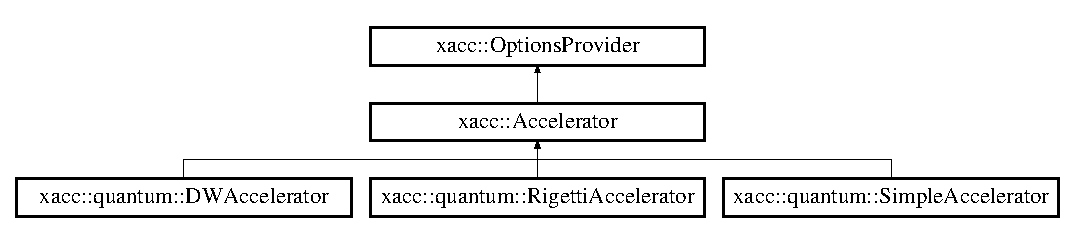
\includegraphics[height=2.679426cm]{a00011}
\end{center}
\end{figure}
\subsection*{Public Member Functions}
\begin{DoxyCompactItemize}
\item 
virtual void \hyperlink{a00011_a8cdc6f0c5a660013c29c07657a06303b}{initialize} ()=0
\item 
virtual Accelerator\+Type \hyperlink{a00011_aaffc3e4bb9880eb5041b1b58ee4c2665}{get\+Type} ()=0
\item 
virtual std\+::vector$<$ \hyperlink{a00051}{I\+R\+Transformation} $>$ \hyperlink{a00011_ad6e4a642dcb24e552675bcbeff1e1b04}{get\+I\+R\+Transformations} ()=0
\item 
virtual void \hyperlink{a00011_a89b3f3e6294f228abf03a410b0fb1674}{execute} (std\+::shared\+\_\+ptr$<$ \hyperlink{a00013}{Accelerator\+Buffer} $>$ buffer, const std\+::shared\+\_\+ptr$<$ \hyperlink{a00038}{Function} $>$ function)=0
\item 
virtual std\+::shared\+\_\+ptr$<$ \hyperlink{a00013}{Accelerator\+Buffer} $>$ \hyperlink{a00011_aab5046e8d83ab390302e0f49533e95fc}{create\+Buffer} (const std\+::string \&var\+Id)=0
\item 
virtual std\+::shared\+\_\+ptr$<$ \hyperlink{a00013}{Accelerator\+Buffer} $>$ \hyperlink{a00011_a064a2dbd58338364115c260267806945}{create\+Buffer} (const std\+::string \&var\+Id, const int size)=0
\item 
virtual std\+::shared\+\_\+ptr$<$ \hyperlink{a00013}{Accelerator\+Buffer} $>$ \hyperlink{a00011_ab3820be326e28a553fed1a824f4d41d0}{get\+Buffer} (const std\+::string \&varid)
\item 
virtual std\+::vector$<$ std\+::string $>$ \hyperlink{a00011_ae1463d7e405df89fa4af47e8922f4b82}{get\+Allocated\+Buffer\+Names} ()
\item 
virtual std\+::shared\+\_\+ptr$<$ \hyperlink{a00043}{Accelerator\+Graph} $>$ \hyperlink{a00011_adfed940ce1fa476b009344ddf5a4bbc3}{get\+Accelerator\+Connectivity} ()
\item 
virtual std\+::shared\+\_\+ptr$<$ options\+\_\+description $>$ \hyperlink{a00011_a98c9eda6b54367c75667ecfbbf167979}{get\+Options} ()
\item 
virtual \hyperlink{a00011_aed88ab0d71b765f0b0f512684ccd4b55}{$\sim$\+Accelerator} ()
\end{DoxyCompactItemize}
\subsection*{Protected Member Functions}
\begin{DoxyCompactItemize}
\item 
virtual bool \hyperlink{a00011_ae51584850faeec77299058383977ddeb}{is\+Valid\+Buffer\+Size} (const int N\+Bits)=0
\item 
void \hyperlink{a00011_ac3e781f42ec25e460174d4c41ea26b94}{store\+Buffer} (const std\+::string \&id, std\+::shared\+\_\+ptr$<$ \hyperlink{a00013}{Accelerator\+Buffer} $>$ b)
\end{DoxyCompactItemize}


\subsection{Detailed Description}
The \hyperlink{a00011}{Accelerator} class provides a high-\/level abstraction for X\+A\+CC\textquotesingle{}s interaction with attached post-\/exascale accelerators (quantum and neuromorphic processing units).

Derived Accelerators must provide a valid execute implementation that takes X\+A\+CC \hyperlink{a00050}{IR} and executes it on the attached hardware or simulator.

Derived Accelerators must provide a list of \hyperlink{a00051}{I\+R\+Transformation} instances that transform X\+A\+CC \hyperlink{a00050}{IR} to be amenable to execution on the hardware.

Derived Accelerators must provide implementations of create\+Buffer that provide a valid \hyperlink{a00013}{Accelerator\+Buffer} instance modeling the hardware memory or bits being computed on. Upon creating an \hyperlink{a00013}{Accelerator\+Buffer}, derived \hyperlink{a00011}{Accelerator} implementations must call the protected store\+Buffer method to store the \hyperlink{a00013}{Accelerator\+Buffer} for future reference by Compilers and clients of \hyperlink{a00011}{Accelerator}.

\begin{DoxyAuthor}{Author}
Alex Mc\+Caskey 
\end{DoxyAuthor}


\subsection{Constructor \& Destructor Documentation}
\index{xacc\+::\+Accelerator@{xacc\+::\+Accelerator}!````~Accelerator@{$\sim$\+Accelerator}}
\index{````~Accelerator@{$\sim$\+Accelerator}!xacc\+::\+Accelerator@{xacc\+::\+Accelerator}}
\subsubsection[{\texorpdfstring{$\sim$\+Accelerator()}{~Accelerator()}}]{\setlength{\rightskip}{0pt plus 5cm}virtual xacc\+::\+Accelerator\+::$\sim$\+Accelerator (
\begin{DoxyParamCaption}
{}
\end{DoxyParamCaption}
)\hspace{0.3cm}{\ttfamily [inline]}, {\ttfamily [virtual]}}\hypertarget{a00011_aed88ab0d71b765f0b0f512684ccd4b55}{}\label{a00011_aed88ab0d71b765f0b0f512684ccd4b55}
Destructor 

\subsection{Member Function Documentation}
\index{xacc\+::\+Accelerator@{xacc\+::\+Accelerator}!create\+Buffer@{create\+Buffer}}
\index{create\+Buffer@{create\+Buffer}!xacc\+::\+Accelerator@{xacc\+::\+Accelerator}}
\subsubsection[{\texorpdfstring{create\+Buffer(const std\+::string \&var\+Id)=0}{createBuffer(const std::string \&varId)=0}}]{\setlength{\rightskip}{0pt plus 5cm}virtual std\+::shared\+\_\+ptr$<${\bf Accelerator\+Buffer}$>$ xacc\+::\+Accelerator\+::create\+Buffer (
\begin{DoxyParamCaption}
\item[{const std\+::string \&}]{var\+Id}
\end{DoxyParamCaption}
)\hspace{0.3cm}{\ttfamily [pure virtual]}}\hypertarget{a00011_aab5046e8d83ab390302e0f49533e95fc}{}\label{a00011_aab5046e8d83ab390302e0f49533e95fc}
Create, store, and return an \hyperlink{a00013}{Accelerator\+Buffer} with the given variable id string. This method returns all available qubits for this \hyperlink{a00011}{Accelerator}. The string id serves as a unique identifier for future lookups and reuse of the \hyperlink{a00013}{Accelerator\+Buffer}.


\begin{DoxyParams}{Parameters}
{\em var\+Id} & The variable name of the created buffer \\
\hline
\end{DoxyParams}
\begin{DoxyReturn}{Returns}
buffer The buffer instance created. 
\end{DoxyReturn}


Implemented in \hyperlink{a00029_add60637a4b3c055e7f2ffa3bf8e320ac}{xacc\+::quantum\+::\+D\+W\+Accelerator}, \hyperlink{a00079_a46445d77d4b8ad2689571d0db6604380}{xacc\+::quantum\+::\+Simple\+Accelerator}, and \hyperlink{a00071_ada3ceb986e51ab5aa721f2a08e083cd6}{xacc\+::quantum\+::\+Rigetti\+Accelerator}.

\index{xacc\+::\+Accelerator@{xacc\+::\+Accelerator}!create\+Buffer@{create\+Buffer}}
\index{create\+Buffer@{create\+Buffer}!xacc\+::\+Accelerator@{xacc\+::\+Accelerator}}
\subsubsection[{\texorpdfstring{create\+Buffer(const std\+::string \&var\+Id, const int size)=0}{createBuffer(const std::string \&varId, const int size)=0}}]{\setlength{\rightskip}{0pt plus 5cm}virtual std\+::shared\+\_\+ptr$<${\bf Accelerator\+Buffer}$>$ xacc\+::\+Accelerator\+::create\+Buffer (
\begin{DoxyParamCaption}
\item[{const std\+::string \&}]{var\+Id, }
\item[{const int}]{size}
\end{DoxyParamCaption}
)\hspace{0.3cm}{\ttfamily [pure virtual]}}\hypertarget{a00011_a064a2dbd58338364115c260267806945}{}\label{a00011_a064a2dbd58338364115c260267806945}
Create, store, and return an \hyperlink{a00013}{Accelerator\+Buffer} with the given variable id string and of the given number of bits. The string id serves as a unique identifier for future lookups and reuse of the \hyperlink{a00013}{Accelerator\+Buffer}.


\begin{DoxyParams}{Parameters}
{\em var\+Id} & The variable name of the created buffer \\
\hline
{\em size} & The number of bits in the created buffer \\
\hline
\end{DoxyParams}
\begin{DoxyReturn}{Returns}
buffer The buffer instance created. 
\end{DoxyReturn}


Implemented in \hyperlink{a00029_a718d7cb51a35e694d960385e1ea2f99f}{xacc\+::quantum\+::\+D\+W\+Accelerator}, \hyperlink{a00071_a731551c94b1abef40d2cf032e8712df6}{xacc\+::quantum\+::\+Rigetti\+Accelerator}, and \hyperlink{a00079_adb9393692e9f484df241aa5d014030d1}{xacc\+::quantum\+::\+Simple\+Accelerator}.

\index{xacc\+::\+Accelerator@{xacc\+::\+Accelerator}!execute@{execute}}
\index{execute@{execute}!xacc\+::\+Accelerator@{xacc\+::\+Accelerator}}
\subsubsection[{\texorpdfstring{execute(std\+::shared\+\_\+ptr$<$ Accelerator\+Buffer $>$ buffer, const std\+::shared\+\_\+ptr$<$ Function $>$ function)=0}{execute(std::shared\_ptr< AcceleratorBuffer > buffer, const std::shared\_ptr< Function > function)=0}}]{\setlength{\rightskip}{0pt plus 5cm}virtual void xacc\+::\+Accelerator\+::execute (
\begin{DoxyParamCaption}
\item[{std\+::shared\+\_\+ptr$<$ {\bf Accelerator\+Buffer} $>$}]{buffer, }
\item[{const std\+::shared\+\_\+ptr$<$ {\bf Function} $>$}]{function}
\end{DoxyParamCaption}
)\hspace{0.3cm}{\ttfamily [pure virtual]}}\hypertarget{a00011_a89b3f3e6294f228abf03a410b0fb1674}{}\label{a00011_a89b3f3e6294f228abf03a410b0fb1674}
Execute the provided X\+A\+CC \hyperlink{a00050}{IR} \hyperlink{a00038}{Function} on the provided \hyperlink{a00013}{Accelerator\+Buffer}.


\begin{DoxyParams}{Parameters}
{\em buffer} & The buffer of bits this \hyperlink{a00011}{Accelerator} should operate on. \\
\hline
{\em function} & The kernel to execute. \\
\hline
\end{DoxyParams}
\index{xacc\+::\+Accelerator@{xacc\+::\+Accelerator}!get\+Accelerator\+Connectivity@{get\+Accelerator\+Connectivity}}
\index{get\+Accelerator\+Connectivity@{get\+Accelerator\+Connectivity}!xacc\+::\+Accelerator@{xacc\+::\+Accelerator}}
\subsubsection[{\texorpdfstring{get\+Accelerator\+Connectivity()}{getAcceleratorConnectivity()}}]{\setlength{\rightskip}{0pt plus 5cm}virtual std\+::shared\+\_\+ptr$<${\bf Accelerator\+Graph}$>$ xacc\+::\+Accelerator\+::get\+Accelerator\+Connectivity (
\begin{DoxyParamCaption}
{}
\end{DoxyParamCaption}
)\hspace{0.3cm}{\ttfamily [inline]}, {\ttfamily [virtual]}}\hypertarget{a00011_adfed940ce1fa476b009344ddf5a4bbc3}{}\label{a00011_adfed940ce1fa476b009344ddf5a4bbc3}
Return the graph structure for this \hyperlink{a00011}{Accelerator}.

\begin{DoxyReturn}{Returns}
connectivity\+Graph The graph structure of this \hyperlink{a00011}{Accelerator} 
\end{DoxyReturn}


Reimplemented in \hyperlink{a00029_a006afa60749790681fc76beddc254926}{xacc\+::quantum\+::\+D\+W\+Accelerator}.

\index{xacc\+::\+Accelerator@{xacc\+::\+Accelerator}!get\+Allocated\+Buffer\+Names@{get\+Allocated\+Buffer\+Names}}
\index{get\+Allocated\+Buffer\+Names@{get\+Allocated\+Buffer\+Names}!xacc\+::\+Accelerator@{xacc\+::\+Accelerator}}
\subsubsection[{\texorpdfstring{get\+Allocated\+Buffer\+Names()}{getAllocatedBufferNames()}}]{\setlength{\rightskip}{0pt plus 5cm}virtual std\+::vector$<$std\+::string$>$ xacc\+::\+Accelerator\+::get\+Allocated\+Buffer\+Names (
\begin{DoxyParamCaption}
{}
\end{DoxyParamCaption}
)\hspace{0.3cm}{\ttfamily [inline]}, {\ttfamily [virtual]}}\hypertarget{a00011_ae1463d7e405df89fa4af47e8922f4b82}{}\label{a00011_ae1463d7e405df89fa4af47e8922f4b82}
Return all allocated \hyperlink{a00013}{Accelerator\+Buffer} variable names.

\begin{DoxyReturn}{Returns}
var\+Names The buffer variable names 
\end{DoxyReturn}
\index{xacc\+::\+Accelerator@{xacc\+::\+Accelerator}!get\+Buffer@{get\+Buffer}}
\index{get\+Buffer@{get\+Buffer}!xacc\+::\+Accelerator@{xacc\+::\+Accelerator}}
\subsubsection[{\texorpdfstring{get\+Buffer(const std\+::string \&varid)}{getBuffer(const std::string \&varid)}}]{\setlength{\rightskip}{0pt plus 5cm}virtual std\+::shared\+\_\+ptr$<${\bf Accelerator\+Buffer}$>$ xacc\+::\+Accelerator\+::get\+Buffer (
\begin{DoxyParamCaption}
\item[{const std\+::string \&}]{varid}
\end{DoxyParamCaption}
)\hspace{0.3cm}{\ttfamily [inline]}, {\ttfamily [virtual]}}\hypertarget{a00011_ab3820be326e28a553fed1a824f4d41d0}{}\label{a00011_ab3820be326e28a553fed1a824f4d41d0}
Return the stored \hyperlink{a00013}{Accelerator\+Buffer} with the provided string id.


\begin{DoxyParams}{Parameters}
{\em varid} & The variable name of the created buffer \\
\hline
\end{DoxyParams}
\begin{DoxyReturn}{Returns}
buffer The buffer with given varid. 
\end{DoxyReturn}
\index{xacc\+::\+Accelerator@{xacc\+::\+Accelerator}!get\+I\+R\+Transformations@{get\+I\+R\+Transformations}}
\index{get\+I\+R\+Transformations@{get\+I\+R\+Transformations}!xacc\+::\+Accelerator@{xacc\+::\+Accelerator}}
\subsubsection[{\texorpdfstring{get\+I\+R\+Transformations()=0}{getIRTransformations()=0}}]{\setlength{\rightskip}{0pt plus 5cm}virtual std\+::vector$<${\bf I\+R\+Transformation}$>$ xacc\+::\+Accelerator\+::get\+I\+R\+Transformations (
\begin{DoxyParamCaption}
{}
\end{DoxyParamCaption}
)\hspace{0.3cm}{\ttfamily [pure virtual]}}\hypertarget{a00011_ad6e4a642dcb24e552675bcbeff1e1b04}{}\label{a00011_ad6e4a642dcb24e552675bcbeff1e1b04}
Return any \hyperlink{a00050}{IR} Transformations that must be applied to ensure the compiled \hyperlink{a00050}{IR} is amenable to execution on this \hyperlink{a00011}{Accelerator}.

\begin{DoxyReturn}{Returns}
transformations The \hyperlink{a00050}{IR} transformations this \hyperlink{a00011}{Accelerator} exposes 
\end{DoxyReturn}


Implemented in \hyperlink{a00029_a89da20bd079a22d6581ea2da2293b973}{xacc\+::quantum\+::\+D\+W\+Accelerator}, \hyperlink{a00071_a443683a1dfb000603c640b2ee303cf66}{xacc\+::quantum\+::\+Rigetti\+Accelerator}, and \hyperlink{a00079_afc49c9e7973ba6c6ff9761c36198323d}{xacc\+::quantum\+::\+Simple\+Accelerator}.

\index{xacc\+::\+Accelerator@{xacc\+::\+Accelerator}!get\+Options@{get\+Options}}
\index{get\+Options@{get\+Options}!xacc\+::\+Accelerator@{xacc\+::\+Accelerator}}
\subsubsection[{\texorpdfstring{get\+Options()}{getOptions()}}]{\setlength{\rightskip}{0pt plus 5cm}virtual std\+::shared\+\_\+ptr$<$options\+\_\+description$>$ xacc\+::\+Accelerator\+::get\+Options (
\begin{DoxyParamCaption}
{}
\end{DoxyParamCaption}
)\hspace{0.3cm}{\ttfamily [inline]}, {\ttfamily [virtual]}}\hypertarget{a00011_a98c9eda6b54367c75667ecfbbf167979}{}\label{a00011_a98c9eda6b54367c75667ecfbbf167979}
Return an empty options\+\_\+description, this is for subclasses to implement. 

Implements \hyperlink{a00056_a6d150954f852109bfe2c1ae90222926f}{xacc\+::\+Options\+Provider}.



Reimplemented in \hyperlink{a00029_a09926db9f99706307ae6ce5b56845bca}{xacc\+::quantum\+::\+D\+W\+Accelerator}, and \hyperlink{a00071_a9ee9e62aecbccf193894ca3388676f9f}{xacc\+::quantum\+::\+Rigetti\+Accelerator}.

\index{xacc\+::\+Accelerator@{xacc\+::\+Accelerator}!get\+Type@{get\+Type}}
\index{get\+Type@{get\+Type}!xacc\+::\+Accelerator@{xacc\+::\+Accelerator}}
\subsubsection[{\texorpdfstring{get\+Type()=0}{getType()=0}}]{\setlength{\rightskip}{0pt plus 5cm}virtual Accelerator\+Type xacc\+::\+Accelerator\+::get\+Type (
\begin{DoxyParamCaption}
{}
\end{DoxyParamCaption}
)\hspace{0.3cm}{\ttfamily [pure virtual]}}\hypertarget{a00011_aaffc3e4bb9880eb5041b1b58ee4c2665}{}\label{a00011_aaffc3e4bb9880eb5041b1b58ee4c2665}
Return the type of this \hyperlink{a00011}{Accelerator}.

\begin{DoxyReturn}{Returns}
type The \hyperlink{a00011}{Accelerator} type -\/ Gate or A\+QC Q\+PU, or N\+PU 
\end{DoxyReturn}


Implemented in \hyperlink{a00029_abe50e427b4bec0460cc238405cb569f9}{xacc\+::quantum\+::\+D\+W\+Accelerator}, \hyperlink{a00071_aab0d4674da5273d55407b9ab77cde890}{xacc\+::quantum\+::\+Rigetti\+Accelerator}, and \hyperlink{a00079_ad76eeb0bbd7de21aad5bd20d20970a98}{xacc\+::quantum\+::\+Simple\+Accelerator}.

\index{xacc\+::\+Accelerator@{xacc\+::\+Accelerator}!initialize@{initialize}}
\index{initialize@{initialize}!xacc\+::\+Accelerator@{xacc\+::\+Accelerator}}
\subsubsection[{\texorpdfstring{initialize()=0}{initialize()=0}}]{\setlength{\rightskip}{0pt plus 5cm}virtual void xacc\+::\+Accelerator\+::initialize (
\begin{DoxyParamCaption}
{}
\end{DoxyParamCaption}
)\hspace{0.3cm}{\ttfamily [pure virtual]}}\hypertarget{a00011_a8cdc6f0c5a660013c29c07657a06303b}{}\label{a00011_a8cdc6f0c5a660013c29c07657a06303b}
Initialize this \hyperlink{a00011}{Accelerator}. This method is called by the X\+A\+CC framework after an \hyperlink{a00011}{Accelerator} has been requested and created. Perform any work you need done before execution here. 

Implemented in \hyperlink{a00029_acaefd5747409f31cf5c3e42d98475ce2}{xacc\+::quantum\+::\+D\+W\+Accelerator}, \hyperlink{a00071_ab8b6af9bb9dcb110201e9ee5cac74b4f}{xacc\+::quantum\+::\+Rigetti\+Accelerator}, and \hyperlink{a00079_a392e3b30523f5f681127e7e98887108c}{xacc\+::quantum\+::\+Simple\+Accelerator}.

\index{xacc\+::\+Accelerator@{xacc\+::\+Accelerator}!is\+Valid\+Buffer\+Size@{is\+Valid\+Buffer\+Size}}
\index{is\+Valid\+Buffer\+Size@{is\+Valid\+Buffer\+Size}!xacc\+::\+Accelerator@{xacc\+::\+Accelerator}}
\subsubsection[{\texorpdfstring{is\+Valid\+Buffer\+Size(const int N\+Bits)=0}{isValidBufferSize(const int NBits)=0}}]{\setlength{\rightskip}{0pt plus 5cm}virtual bool xacc\+::\+Accelerator\+::is\+Valid\+Buffer\+Size (
\begin{DoxyParamCaption}
\item[{const int}]{N\+Bits}
\end{DoxyParamCaption}
)\hspace{0.3cm}{\ttfamily [protected]}, {\ttfamily [pure virtual]}}\hypertarget{a00011_ae51584850faeec77299058383977ddeb}{}\label{a00011_ae51584850faeec77299058383977ddeb}
Return true if this \hyperlink{a00011}{Accelerator} can allocated N\+Bits number of bits. This is meant to be implemented and used by subclasses.


\begin{DoxyParams}{Parameters}
{\em N\+Bits} & The number of bits to allocate \\
\hline
\end{DoxyParams}
\begin{DoxyReturn}{Returns}
valid True if size is valid. 
\end{DoxyReturn}


Implemented in \hyperlink{a00029_a4c2ee30212a919d8ddf7f9555df25195}{xacc\+::quantum\+::\+D\+W\+Accelerator}, \hyperlink{a00079_a60b9db2d6aed235857c45413a070338e}{xacc\+::quantum\+::\+Simple\+Accelerator}, and \hyperlink{a00071_a61352c07062597aad2393fbeed4cc025}{xacc\+::quantum\+::\+Rigetti\+Accelerator}.

\index{xacc\+::\+Accelerator@{xacc\+::\+Accelerator}!store\+Buffer@{store\+Buffer}}
\index{store\+Buffer@{store\+Buffer}!xacc\+::\+Accelerator@{xacc\+::\+Accelerator}}
\subsubsection[{\texorpdfstring{store\+Buffer(const std\+::string \&id, std\+::shared\+\_\+ptr$<$ Accelerator\+Buffer $>$ b)}{storeBuffer(const std::string \&id, std::shared\_ptr< AcceleratorBuffer > b)}}]{\setlength{\rightskip}{0pt plus 5cm}void xacc\+::\+Accelerator\+::store\+Buffer (
\begin{DoxyParamCaption}
\item[{const std\+::string \&}]{id, }
\item[{std\+::shared\+\_\+ptr$<$ {\bf Accelerator\+Buffer} $>$}]{b}
\end{DoxyParamCaption}
)\hspace{0.3cm}{\ttfamily [inline]}, {\ttfamily [protected]}}\hypertarget{a00011_ac3e781f42ec25e460174d4c41ea26b94}{}\label{a00011_ac3e781f42ec25e460174d4c41ea26b94}
This protected method is to be used by derived Accelerators to store any created \hyperlink{a00013}{Accelerator\+Buffer}.


\begin{DoxyParams}{Parameters}
{\em id} & The variable name of the buffer to store \\
\hline
{\em b} & The buffer to store \\
\hline
\end{DoxyParams}


The documentation for this class was generated from the following file\+:\begin{DoxyCompactItemize}
\item 
Accelerator.\+hpp\end{DoxyCompactItemize}

\hypertarget{a00012}{}\section{xacc\+:\+:Accelerator\+Bit Class Reference}
\label{a00012}\index{xacc\+::\+Accelerator\+Bit@{xacc\+::\+Accelerator\+Bit}}


{\ttfamily \#include $<$Accelerator\+Buffer.\+hpp$>$}

\subsection*{Public Member Functions}
\begin{DoxyCompactItemize}
\item 
\hyperlink{a00012_a9a124c230c5cabeab53bac0820c0221a}{Accelerator\+Bit} ()
\item 
void \hyperlink{a00012_aa63a24980e831b9325a36836ab1c5495}{update} (int zero\+Or\+One)
\item 
Accelerator\+Bit\+State \hyperlink{a00012_a4a8dcc4fa02a5619f583961460c77057}{get\+State} ()
\end{DoxyCompactItemize}
\subsection*{Protected Attributes}
\begin{DoxyCompactItemize}
\item 
Accelerator\+Bit\+State \hyperlink{a00012_a4632123ac31aeed0dc97c65f8c792a85}{state}
\end{DoxyCompactItemize}


\subsection{Detailed Description}
The \hyperlink{a00012}{Accelerator\+Bit} wraps an Accelerator\+Bit\+Sate and provides a mechanism for updating that state.

\begin{DoxyAuthor}{Author}
Alex Mc\+Caskey 
\end{DoxyAuthor}


\subsection{Constructor \& Destructor Documentation}
\index{xacc\+::\+Accelerator\+Bit@{xacc\+::\+Accelerator\+Bit}!Accelerator\+Bit@{Accelerator\+Bit}}
\index{Accelerator\+Bit@{Accelerator\+Bit}!xacc\+::\+Accelerator\+Bit@{xacc\+::\+Accelerator\+Bit}}
\subsubsection[{\texorpdfstring{Accelerator\+Bit()}{AcceleratorBit()}}]{\setlength{\rightskip}{0pt plus 5cm}xacc\+::\+Accelerator\+Bit\+::\+Accelerator\+Bit (
\begin{DoxyParamCaption}
{}
\end{DoxyParamCaption}
)\hspace{0.3cm}{\ttfamily [inline]}}\hypertarget{a00012_a9a124c230c5cabeab53bac0820c0221a}{}\label{a00012_a9a124c230c5cabeab53bac0820c0221a}
The constructor, all bits are initialized to unknown state 

\subsection{Member Function Documentation}
\index{xacc\+::\+Accelerator\+Bit@{xacc\+::\+Accelerator\+Bit}!get\+State@{get\+State}}
\index{get\+State@{get\+State}!xacc\+::\+Accelerator\+Bit@{xacc\+::\+Accelerator\+Bit}}
\subsubsection[{\texorpdfstring{get\+State()}{getState()}}]{\setlength{\rightskip}{0pt plus 5cm}Accelerator\+Bit\+State xacc\+::\+Accelerator\+Bit\+::get\+State (
\begin{DoxyParamCaption}
{}
\end{DoxyParamCaption}
)\hspace{0.3cm}{\ttfamily [inline]}}\hypertarget{a00012_a4a8dcc4fa02a5619f583961460c77057}{}\label{a00012_a4a8dcc4fa02a5619f583961460c77057}
Return the value of this state \index{xacc\+::\+Accelerator\+Bit@{xacc\+::\+Accelerator\+Bit}!update@{update}}
\index{update@{update}!xacc\+::\+Accelerator\+Bit@{xacc\+::\+Accelerator\+Bit}}
\subsubsection[{\texorpdfstring{update(int zero\+Or\+One)}{update(int zeroOrOne)}}]{\setlength{\rightskip}{0pt plus 5cm}void xacc\+::\+Accelerator\+Bit\+::update (
\begin{DoxyParamCaption}
\item[{int}]{zero\+Or\+One}
\end{DoxyParamCaption}
)\hspace{0.3cm}{\ttfamily [inline]}}\hypertarget{a00012_aa63a24980e831b9325a36836ab1c5495}{}\label{a00012_aa63a24980e831b9325a36836ab1c5495}
Update the Bit state to a one or zero 

\subsection{Member Data Documentation}
\index{xacc\+::\+Accelerator\+Bit@{xacc\+::\+Accelerator\+Bit}!state@{state}}
\index{state@{state}!xacc\+::\+Accelerator\+Bit@{xacc\+::\+Accelerator\+Bit}}
\subsubsection[{\texorpdfstring{state}{state}}]{\setlength{\rightskip}{0pt plus 5cm}Accelerator\+Bit\+State xacc\+::\+Accelerator\+Bit\+::state\hspace{0.3cm}{\ttfamily [protected]}}\hypertarget{a00012_a4632123ac31aeed0dc97c65f8c792a85}{}\label{a00012_a4632123ac31aeed0dc97c65f8c792a85}
The bit state 

The documentation for this class was generated from the following file\+:\begin{DoxyCompactItemize}
\item 
Accelerator\+Buffer.\+hpp\end{DoxyCompactItemize}

\hypertarget{a00013}{}\section{xacc\+:\+:Accelerator\+Buffer Class Reference}
\label{a00013}\index{xacc\+::\+Accelerator\+Buffer@{xacc\+::\+Accelerator\+Buffer}}


{\ttfamily \#include $<$Accelerator\+Buffer.\+hpp$>$}

Inheritance diagram for xacc\+:\+:Accelerator\+Buffer\+:\begin{figure}[H]
\begin{center}
\leavevmode
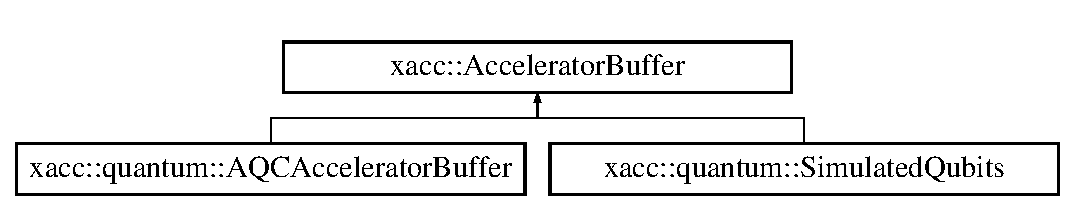
\includegraphics[height=2.000000cm]{a00013}
\end{center}
\end{figure}
\subsection*{Public Member Functions}
\begin{DoxyCompactItemize}
\item 
\hyperlink{a00013_ab606d8af942120d60b51a4fffcd75c98}{Accelerator\+Buffer} (const std\+::string \&str, const int N)
\item 
{\footnotesize template$<$typename... Indices$>$ }\\{\bfseries Accelerator\+Buffer} (const std\+::string \&str, int first\+Index, Indices...\+indices)\hypertarget{a00013_ac550d89390562095c56aa1b14ae85001}{}\label{a00013_ac550d89390562095c56aa1b14ae85001}

\item 
int {\bfseries size} ()\hypertarget{a00013_aa2a3101c2e3ae3550172bf49f9587f3b}{}\label{a00013_aa2a3101c2e3ae3550172bf49f9587f3b}

\item 
std\+::string {\bfseries name} ()\hypertarget{a00013_ad5b646e9efc21b6d0bcc22cd6f649c22}{}\label{a00013_ad5b646e9efc21b6d0bcc22cd6f649c22}

\item 
void {\bfseries reset\+Buffer} ()\hypertarget{a00013_aa6d6e9cfee6170333c1f03507345743f}{}\label{a00013_aa6d6e9cfee6170333c1f03507345743f}

\item 
void {\bfseries update\+Bit} (const int idx, int zero\+Or\+One)\hypertarget{a00013_a4bc0edbe9aa0d463f67ddcc38265066f}{}\label{a00013_a4bc0edbe9aa0d463f67ddcc38265066f}

\item 
void {\bfseries append\+Measurement} (const boost\+::dynamic\+\_\+bitset$<$$>$ \&measurement)\hypertarget{a00013_ac161c4f984f774d08197871094aabc67}{}\label{a00013_ac161c4f984f774d08197871094aabc67}

\item 
double {\bfseries get\+Average} () const \hypertarget{a00013_a97cf3cc4e1aaa8ac3cee7817860f77c1}{}\label{a00013_a97cf3cc4e1aaa8ac3cee7817860f77c1}

\item 
Accelerator\+Bit\+State {\bfseries get\+Accelerator\+Bit\+State} (const int idx)\hypertarget{a00013_aba6ef359f3117faa98f0eb8da90d909e}{}\label{a00013_aba6ef359f3117faa98f0eb8da90d909e}

\item 
virtual void {\bfseries print} ()\hypertarget{a00013_add0835e188f0eda4f1b68a28ddc79786}{}\label{a00013_add0835e188f0eda4f1b68a28ddc79786}

\item 
virtual void {\bfseries print} (std\+::ostream \&stream)\hypertarget{a00013_a7c59462451223772b41ef232b06a7dfa}{}\label{a00013_a7c59462451223772b41ef232b06a7dfa}

\end{DoxyCompactItemize}
\subsection*{Protected Attributes}
\begin{DoxyCompactItemize}
\item 
std\+::vector$<$ boost\+::dynamic\+\_\+bitset$<$$>$ $>$ {\bfseries measurements}\hypertarget{a00013_a5464b23a964985df2547f657877c9ea5}{}\label{a00013_a5464b23a964985df2547f657877c9ea5}

\item 
std\+::string {\bfseries buffer\+Id}\hypertarget{a00013_a3198e034d07d9b77b62da03e6592a221}{}\label{a00013_a3198e034d07d9b77b62da03e6592a221}

\item 
std\+::vector$<$ \hyperlink{a00012}{Accelerator\+Bit} $>$ {\bfseries bits}\hypertarget{a00013_ab6dbb8c22f8adc6aba34b00a84066854}{}\label{a00013_ab6dbb8c22f8adc6aba34b00a84066854}

\end{DoxyCompactItemize}


\subsection{Detailed Description}
The \hyperlink{a00013}{Accelerator\+Buffer} models an allocated buffer of bits that are operated on by a kernel. As such, the \hyperlink{a00013}{Accelerator\+Buffer}\textquotesingle{}s primary role is to store \hyperlink{a00011}{Accelerator} execution results.

\begin{DoxyAuthor}{Author}
Alex Mc\+Caskey 
\end{DoxyAuthor}


\subsection{Constructor \& Destructor Documentation}
\index{xacc\+::\+Accelerator\+Buffer@{xacc\+::\+Accelerator\+Buffer}!Accelerator\+Buffer@{Accelerator\+Buffer}}
\index{Accelerator\+Buffer@{Accelerator\+Buffer}!xacc\+::\+Accelerator\+Buffer@{xacc\+::\+Accelerator\+Buffer}}
\subsubsection[{\texorpdfstring{Accelerator\+Buffer(const std\+::string \&str, const int N)}{AcceleratorBuffer(const std::string \&str, const int N)}}]{\setlength{\rightskip}{0pt plus 5cm}xacc\+::\+Accelerator\+Buffer\+::\+Accelerator\+Buffer (
\begin{DoxyParamCaption}
\item[{const std\+::string \&}]{str, }
\item[{const int}]{N}
\end{DoxyParamCaption}
)\hspace{0.3cm}{\ttfamily [inline]}}\hypertarget{a00013_ab606d8af942120d60b51a4fffcd75c98}{}\label{a00013_ab606d8af942120d60b51a4fffcd75c98}
The Constructor 

The documentation for this class was generated from the following file\+:\begin{DoxyCompactItemize}
\item 
Accelerator\+Buffer.\+hpp\end{DoxyCompactItemize}

\hypertarget{a00014}{}\section{xacc\+:\+:Algorithm\+Generator Class Reference}
\label{a00014}\index{xacc\+::\+Algorithm\+Generator@{xacc\+::\+Algorithm\+Generator}}


{\ttfamily \#include $<$Algorithm\+Generator.\+hpp$>$}

Inheritance diagram for xacc\+:\+:Algorithm\+Generator\+:\begin{figure}[H]
\begin{center}
\leavevmode
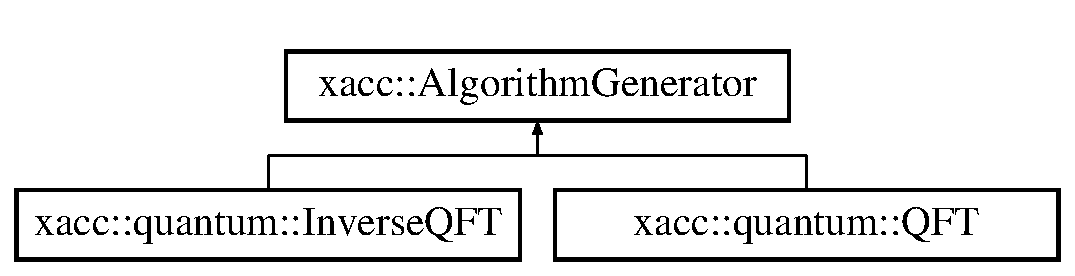
\includegraphics[height=2.000000cm]{a00014}
\end{center}
\end{figure}
\subsection*{Public Member Functions}
\begin{DoxyCompactItemize}
\item 
virtual std\+::shared\+\_\+ptr$<$ \hyperlink{a00038}{Function} $>$ \hyperlink{a00014_a73023c06f0f0c62ad56ab4187b18b096}{generate\+Algorithm} (std\+::vector$<$ int $>$ bits)=0
\item 
virtual \hyperlink{a00014_a096f66aa8d65f5aa3276915768159579}{$\sim$\+Algorithm\+Generator} ()
\end{DoxyCompactItemize}


\subsection{Detailed Description}
The \hyperlink{a00014}{Algorithm\+Generator} interface provides a mechanism for generating algorithms modeled as an X\+A\+CC \hyperlink{a00038}{Function} instance.

\begin{DoxyAuthor}{Author}
Alex Mc\+Caskey 
\end{DoxyAuthor}


\subsection{Constructor \& Destructor Documentation}
\index{xacc\+::\+Algorithm\+Generator@{xacc\+::\+Algorithm\+Generator}!````~Algorithm\+Generator@{$\sim$\+Algorithm\+Generator}}
\index{````~Algorithm\+Generator@{$\sim$\+Algorithm\+Generator}!xacc\+::\+Algorithm\+Generator@{xacc\+::\+Algorithm\+Generator}}
\subsubsection[{\texorpdfstring{$\sim$\+Algorithm\+Generator()}{~AlgorithmGenerator()}}]{\setlength{\rightskip}{0pt plus 5cm}virtual xacc\+::\+Algorithm\+Generator\+::$\sim$\+Algorithm\+Generator (
\begin{DoxyParamCaption}
{}
\end{DoxyParamCaption}
)\hspace{0.3cm}{\ttfamily [inline]}, {\ttfamily [virtual]}}\hypertarget{a00014_a096f66aa8d65f5aa3276915768159579}{}\label{a00014_a096f66aa8d65f5aa3276915768159579}
The destructor 

\subsection{Member Function Documentation}
\index{xacc\+::\+Algorithm\+Generator@{xacc\+::\+Algorithm\+Generator}!generate\+Algorithm@{generate\+Algorithm}}
\index{generate\+Algorithm@{generate\+Algorithm}!xacc\+::\+Algorithm\+Generator@{xacc\+::\+Algorithm\+Generator}}
\subsubsection[{\texorpdfstring{generate\+Algorithm(std\+::vector$<$ int $>$ bits)=0}{generateAlgorithm(std::vector< int > bits)=0}}]{\setlength{\rightskip}{0pt plus 5cm}virtual std\+::shared\+\_\+ptr$<${\bf Function}$>$ xacc\+::\+Algorithm\+Generator\+::generate\+Algorithm (
\begin{DoxyParamCaption}
\item[{std\+::vector$<$ int $>$}]{bits}
\end{DoxyParamCaption}
)\hspace{0.3cm}{\ttfamily [pure virtual]}}\hypertarget{a00014_a73023c06f0f0c62ad56ab4187b18b096}{}\label{a00014_a73023c06f0f0c62ad56ab4187b18b096}
Implementations of this method generate a \hyperlink{a00038}{Function} \hyperlink{a00050}{IR} instance corresponding to the implementation\textquotesingle{}s modeled algorithm. The algorithm is specified to operate over the provided bits.


\begin{DoxyParams}{Parameters}
{\em bits} & The bits this algorithm operates on \\
\hline
\end{DoxyParams}
\begin{DoxyReturn}{Returns}
function The algorithm represented as an \hyperlink{a00050}{IR} \hyperlink{a00038}{Function} 
\end{DoxyReturn}


Implemented in \hyperlink{a00060_ac093c288bc9fc069464fc3fd2cc0ac21}{xacc\+::quantum\+::\+Q\+FT}, and \hyperlink{a00049_af42e466bf02dbd60670d20aa55cfb08d}{xacc\+::quantum\+::\+Inverse\+Q\+FT}.



The documentation for this class was generated from the following file\+:\begin{DoxyCompactItemize}
\item 
Algorithm\+Generator.\+hpp\end{DoxyCompactItemize}

\hypertarget{a00015}{}\section{xacc\+:\+:quantum\+:\+:All\+Gate\+Visitor Class Reference}
\label{a00015}\index{xacc\+::quantum\+::\+All\+Gate\+Visitor@{xacc\+::quantum\+::\+All\+Gate\+Visitor}}


{\ttfamily \#include $<$All\+Gate\+Visitor.\+hpp$>$}

Inheritance diagram for xacc\+:\+:quantum\+:\+:All\+Gate\+Visitor\+:\begin{figure}[H]
\begin{center}
\leavevmode
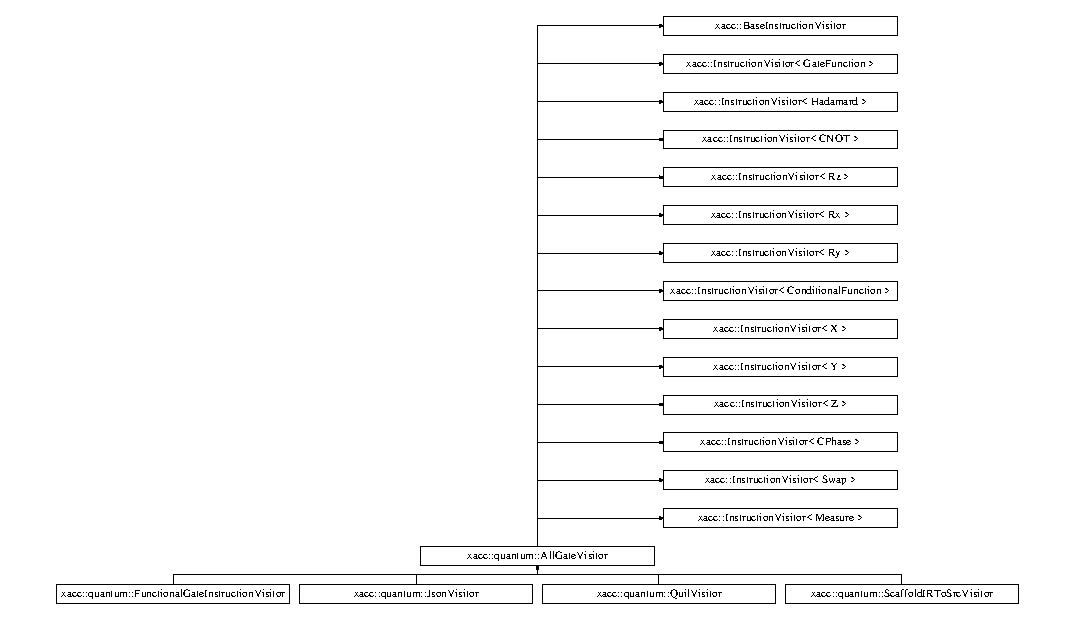
\includegraphics[height=7.887324cm]{a00015}
\end{center}
\end{figure}
\subsection*{Additional Inherited Members}


\subsection{Detailed Description}
F\+I\+X\+ME write this 

The documentation for this class was generated from the following file\+:\begin{DoxyCompactItemize}
\item 
All\+Gate\+Visitor.\+hpp\end{DoxyCompactItemize}

\hypertarget{a00016}{}\section{xacc\+:\+:quantum\+:\+:A\+Q\+C\+Accelerator\+Buffer Class Reference}
\label{a00016}\index{xacc\+::quantum\+::\+A\+Q\+C\+Accelerator\+Buffer@{xacc\+::quantum\+::\+A\+Q\+C\+Accelerator\+Buffer}}


{\ttfamily \#include $<$A\+Q\+C\+Accelerator\+Buffer.\+hpp$>$}

Inheritance diagram for xacc\+:\+:quantum\+:\+:A\+Q\+C\+Accelerator\+Buffer\+:\begin{figure}[H]
\begin{center}
\leavevmode
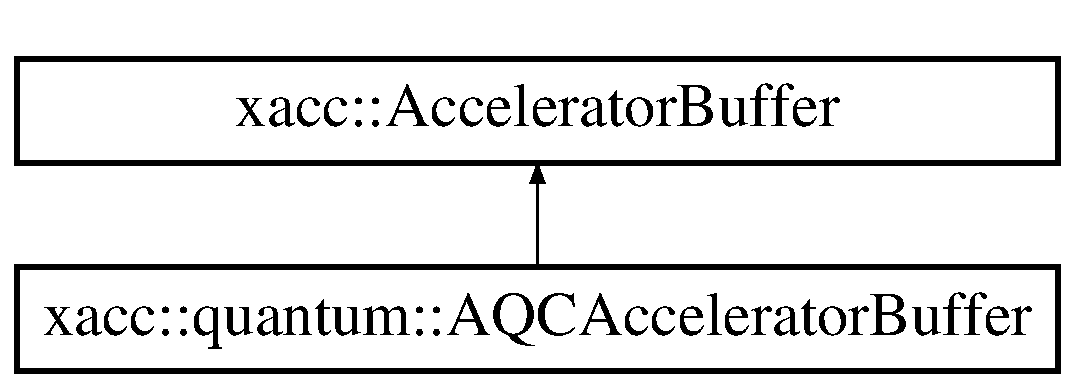
\includegraphics[height=2.000000cm]{a00016}
\end{center}
\end{figure}
\subsection*{Public Member Functions}
\begin{DoxyCompactItemize}
\item 
\hyperlink{a00016_ac2f9ea58140a27741b4dc8fceaa1ca5c}{A\+Q\+C\+Accelerator\+Buffer} (const std\+::string \&str, const int N)
\item 
{\footnotesize template$<$typename... Indices$>$ }\\\hyperlink{a00016_a628c742acf1d20fc8fe9b69f9be7b2c6}{A\+Q\+C\+Accelerator\+Buffer} (const std\+::string \&str, int first\+Index, Indices...\+indices)
\item 
void \hyperlink{a00016_a23992d11bdb6f093c0ce3f743677d4d9}{set\+Embedding} (std\+::map$<$ int, std\+::list$<$ int $>$$>$ emb)
\item 
std\+::map$<$ int, std\+::list$<$ int $>$ $>$ \hyperlink{a00016_ae98155c023d1b31b3b55a8c8e4ec6bc6}{get\+Embedding} ()
\end{DoxyCompactItemize}
\subsection*{Protected Attributes}
\begin{DoxyCompactItemize}
\item 
std\+::map$<$ int, std\+::list$<$ int $>$ $>$ \hyperlink{a00016_a26fd739244b0346cc3398eef31b11264}{embedding}
\item 
std\+::vector$<$ double $>$ \hyperlink{a00016_abe6d781724e197df449d8dfcde60e1a4}{energies}
\end{DoxyCompactItemize}


\subsection{Detailed Description}
The \hyperlink{a00016}{A\+Q\+C\+Accelerator\+Buffer} is an \hyperlink{a00013}{Accelerator\+Buffer} that keeps track of the problem-\/specific embedding into the hardware graph. It also tracks A\+QC Q\+PU computed energies. 

\subsection{Constructor \& Destructor Documentation}
\index{xacc\+::quantum\+::\+A\+Q\+C\+Accelerator\+Buffer@{xacc\+::quantum\+::\+A\+Q\+C\+Accelerator\+Buffer}!A\+Q\+C\+Accelerator\+Buffer@{A\+Q\+C\+Accelerator\+Buffer}}
\index{A\+Q\+C\+Accelerator\+Buffer@{A\+Q\+C\+Accelerator\+Buffer}!xacc\+::quantum\+::\+A\+Q\+C\+Accelerator\+Buffer@{xacc\+::quantum\+::\+A\+Q\+C\+Accelerator\+Buffer}}
\subsubsection[{\texorpdfstring{A\+Q\+C\+Accelerator\+Buffer(const std\+::string \&str, const int N)}{AQCAcceleratorBuffer(const std::string \&str, const int N)}}]{\setlength{\rightskip}{0pt plus 5cm}xacc\+::quantum\+::\+A\+Q\+C\+Accelerator\+Buffer\+::\+A\+Q\+C\+Accelerator\+Buffer (
\begin{DoxyParamCaption}
\item[{const std\+::string \&}]{str, }
\item[{const int}]{N}
\end{DoxyParamCaption}
)\hspace{0.3cm}{\ttfamily [inline]}}\hypertarget{a00016_ac2f9ea58140a27741b4dc8fceaa1ca5c}{}\label{a00016_ac2f9ea58140a27741b4dc8fceaa1ca5c}
The constructor 
\begin{DoxyParams}{Parameters}
{\em str} & The name of this buffer \\
\hline
{\em N} & The number of bits represented by this buffer \\
\hline
\end{DoxyParams}
\index{xacc\+::quantum\+::\+A\+Q\+C\+Accelerator\+Buffer@{xacc\+::quantum\+::\+A\+Q\+C\+Accelerator\+Buffer}!A\+Q\+C\+Accelerator\+Buffer@{A\+Q\+C\+Accelerator\+Buffer}}
\index{A\+Q\+C\+Accelerator\+Buffer@{A\+Q\+C\+Accelerator\+Buffer}!xacc\+::quantum\+::\+A\+Q\+C\+Accelerator\+Buffer@{xacc\+::quantum\+::\+A\+Q\+C\+Accelerator\+Buffer}}
\subsubsection[{\texorpdfstring{A\+Q\+C\+Accelerator\+Buffer(const std\+::string \&str, int first\+Index, Indices...\+indices)}{AQCAcceleratorBuffer(const std::string \&str, int firstIndex, Indices...indices)}}]{\setlength{\rightskip}{0pt plus 5cm}template$<$typename... Indices$>$ xacc\+::quantum\+::\+A\+Q\+C\+Accelerator\+Buffer\+::\+A\+Q\+C\+Accelerator\+Buffer (
\begin{DoxyParamCaption}
\item[{const std\+::string \&}]{str, }
\item[{int}]{first\+Index, }
\item[{Indices...}]{indices}
\end{DoxyParamCaption}
)\hspace{0.3cm}{\ttfamily [inline]}}\hypertarget{a00016_a628c742acf1d20fc8fe9b69f9be7b2c6}{}\label{a00016_a628c742acf1d20fc8fe9b69f9be7b2c6}
The constructor 
\begin{DoxyParams}{Parameters}
{\em str} & \\
\hline
{\em first\+Index} & \\
\hline
{\em indices} & \\
\hline
\end{DoxyParams}


\subsection{Member Function Documentation}
\index{xacc\+::quantum\+::\+A\+Q\+C\+Accelerator\+Buffer@{xacc\+::quantum\+::\+A\+Q\+C\+Accelerator\+Buffer}!get\+Embedding@{get\+Embedding}}
\index{get\+Embedding@{get\+Embedding}!xacc\+::quantum\+::\+A\+Q\+C\+Accelerator\+Buffer@{xacc\+::quantum\+::\+A\+Q\+C\+Accelerator\+Buffer}}
\subsubsection[{\texorpdfstring{get\+Embedding()}{getEmbedding()}}]{\setlength{\rightskip}{0pt plus 5cm}std\+::map$<$int, std\+::list$<$int$>$ $>$ xacc\+::quantum\+::\+A\+Q\+C\+Accelerator\+Buffer\+::get\+Embedding (
\begin{DoxyParamCaption}
{}
\end{DoxyParamCaption}
)\hspace{0.3cm}{\ttfamily [inline]}}\hypertarget{a00016_ae98155c023d1b31b3b55a8c8e4ec6bc6}{}\label{a00016_ae98155c023d1b31b3b55a8c8e4ec6bc6}
Return the minor graph embedding.

\begin{DoxyReturn}{Returns}
emb The minor graph embedding 
\end{DoxyReturn}
\index{xacc\+::quantum\+::\+A\+Q\+C\+Accelerator\+Buffer@{xacc\+::quantum\+::\+A\+Q\+C\+Accelerator\+Buffer}!set\+Embedding@{set\+Embedding}}
\index{set\+Embedding@{set\+Embedding}!xacc\+::quantum\+::\+A\+Q\+C\+Accelerator\+Buffer@{xacc\+::quantum\+::\+A\+Q\+C\+Accelerator\+Buffer}}
\subsubsection[{\texorpdfstring{set\+Embedding(std\+::map$<$ int, std\+::list$<$ int $>$$>$ emb)}{setEmbedding(std::map< int, std::list< int >> emb)}}]{\setlength{\rightskip}{0pt plus 5cm}void xacc\+::quantum\+::\+A\+Q\+C\+Accelerator\+Buffer\+::set\+Embedding (
\begin{DoxyParamCaption}
\item[{std\+::map$<$ int, std\+::list$<$ int $>$$>$}]{emb}
\end{DoxyParamCaption}
)\hspace{0.3cm}{\ttfamily [inline]}}\hypertarget{a00016_a23992d11bdb6f093c0ce3f743677d4d9}{}\label{a00016_a23992d11bdb6f093c0ce3f743677d4d9}
Set the minor graph embedding for the problem solved during this execution .


\begin{DoxyParams}{Parameters}
{\em emb} & The minor graph embedding \\
\hline
\end{DoxyParams}


\subsection{Member Data Documentation}
\index{xacc\+::quantum\+::\+A\+Q\+C\+Accelerator\+Buffer@{xacc\+::quantum\+::\+A\+Q\+C\+Accelerator\+Buffer}!embedding@{embedding}}
\index{embedding@{embedding}!xacc\+::quantum\+::\+A\+Q\+C\+Accelerator\+Buffer@{xacc\+::quantum\+::\+A\+Q\+C\+Accelerator\+Buffer}}
\subsubsection[{\texorpdfstring{embedding}{embedding}}]{\setlength{\rightskip}{0pt plus 5cm}std\+::map$<$int, std\+::list$<$int$>$ $>$ xacc\+::quantum\+::\+A\+Q\+C\+Accelerator\+Buffer\+::embedding\hspace{0.3cm}{\ttfamily [protected]}}\hypertarget{a00016_a26fd739244b0346cc3398eef31b11264}{}\label{a00016_a26fd739244b0346cc3398eef31b11264}
The minor graph embedding for the problem these results represent. \index{xacc\+::quantum\+::\+A\+Q\+C\+Accelerator\+Buffer@{xacc\+::quantum\+::\+A\+Q\+C\+Accelerator\+Buffer}!energies@{energies}}
\index{energies@{energies}!xacc\+::quantum\+::\+A\+Q\+C\+Accelerator\+Buffer@{xacc\+::quantum\+::\+A\+Q\+C\+Accelerator\+Buffer}}
\subsubsection[{\texorpdfstring{energies}{energies}}]{\setlength{\rightskip}{0pt plus 5cm}std\+::vector$<$double$>$ xacc\+::quantum\+::\+A\+Q\+C\+Accelerator\+Buffer\+::energies\hspace{0.3cm}{\ttfamily [protected]}}\hypertarget{a00016_abe6d781724e197df449d8dfcde60e1a4}{}\label{a00016_abe6d781724e197df449d8dfcde60e1a4}
The energies computed as part of this execution. 

The documentation for this class was generated from the following file\+:\begin{DoxyCompactItemize}
\item 
A\+Q\+C\+Accelerator\+Buffer.\+hpp\end{DoxyCompactItemize}

\hypertarget{a00017}{}\section{xacc\+:\+:Base\+Instruction\+Visitable Class Reference}
\label{a00017}\index{xacc\+::\+Base\+Instruction\+Visitable@{xacc\+::\+Base\+Instruction\+Visitable}}


{\ttfamily \#include $<$Instruction\+Visitor.\+hpp$>$}

Inheritance diagram for xacc\+:\+:Base\+Instruction\+Visitable\+:\begin{figure}[H]
\begin{center}
\leavevmode
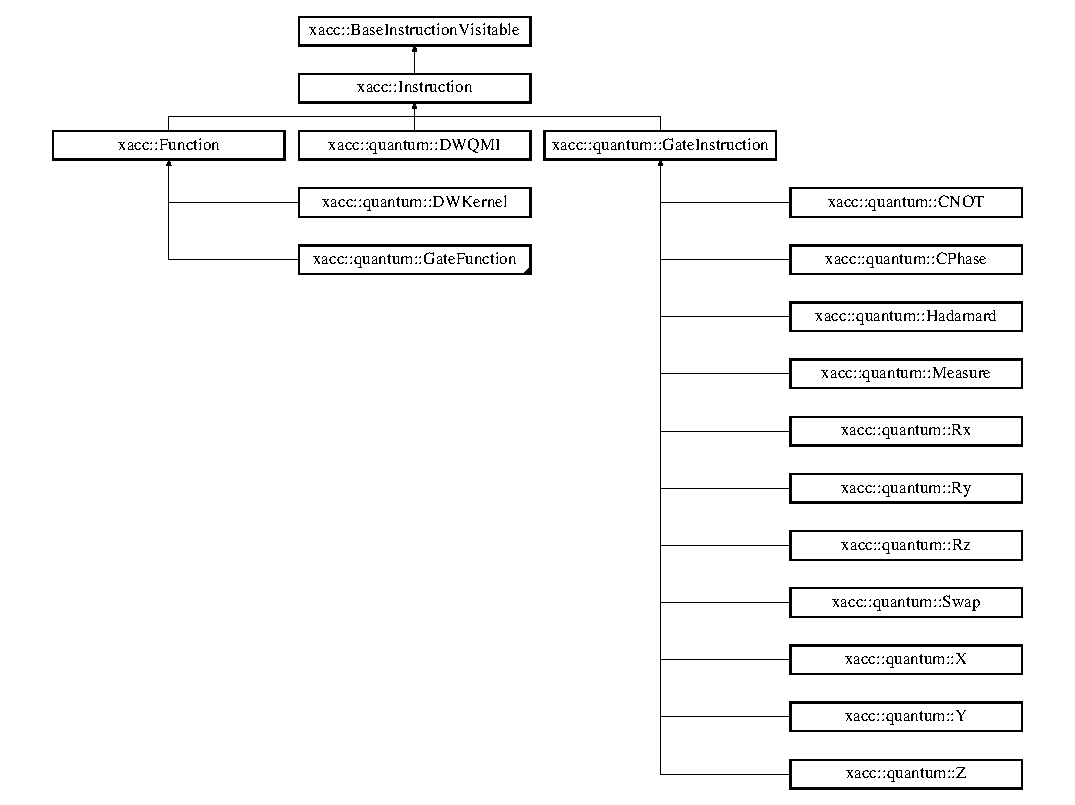
\includegraphics[height=10.370370cm]{a00017}
\end{center}
\end{figure}
\subsection*{Public Member Functions}
\begin{DoxyCompactItemize}
\item 
virtual void \hyperlink{a00017_a4ae295a7f83d57c6f1f912adc90274ea}{accept} (std\+::shared\+\_\+ptr$<$ \hyperlink{a00018}{Base\+Instruction\+Visitor} $>$ visitor)=0
\item 
virtual void \hyperlink{a00017_ad6b9ad95c14580cc86ca87cd464262c3}{accept} (\hyperlink{a00018}{Base\+Instruction\+Visitor} $\ast$visitor)=0
\item 
virtual \hyperlink{a00017_a3a291d247b18ea7620dd8d97dfb595f4}{$\sim$\+Base\+Instruction\+Visitable} ()
\end{DoxyCompactItemize}
\subsection*{Static Protected Member Functions}
\begin{DoxyCompactItemize}
\item 
{\footnotesize template$<$class T $>$ }\\static void \hyperlink{a00017_a2f18b9fcb48f42d190a9f5180b7b59c5}{accept\+Impl} (T \&visited, std\+::shared\+\_\+ptr$<$ \hyperlink{a00018}{Base\+Instruction\+Visitor} $>$ visitor)
\item 
{\footnotesize template$<$class T $>$ }\\static void \hyperlink{a00017_a80c7bb995faa54644f822fa48176c6cb}{accept\+Impl} (T \&visited, \hyperlink{a00018}{Base\+Instruction\+Visitor} $\ast$visitor)
\end{DoxyCompactItemize}


\subsection{Detailed Description}
\hyperlink{a00017}{Base\+Instruction\+Visitable} is an interface that is to be implemented by any and all Instructions that want to be available for visitation. Derivations of this class simply inherit from \hyperlink{a00017}{Base\+Instruction\+Visitable} and declare the D\+E\+F\+I\+N\+E\+\_\+\+V\+I\+S\+I\+T\+A\+B\+LE macro alongside the rest of the classes member methods. 

\subsection{Constructor \& Destructor Documentation}
\index{xacc\+::\+Base\+Instruction\+Visitable@{xacc\+::\+Base\+Instruction\+Visitable}!````~Base\+Instruction\+Visitable@{$\sim$\+Base\+Instruction\+Visitable}}
\index{````~Base\+Instruction\+Visitable@{$\sim$\+Base\+Instruction\+Visitable}!xacc\+::\+Base\+Instruction\+Visitable@{xacc\+::\+Base\+Instruction\+Visitable}}
\subsubsection[{\texorpdfstring{$\sim$\+Base\+Instruction\+Visitable()}{~BaseInstructionVisitable()}}]{\setlength{\rightskip}{0pt plus 5cm}virtual xacc\+::\+Base\+Instruction\+Visitable\+::$\sim$\+Base\+Instruction\+Visitable (
\begin{DoxyParamCaption}
{}
\end{DoxyParamCaption}
)\hspace{0.3cm}{\ttfamily [inline]}, {\ttfamily [virtual]}}\hypertarget{a00017_a3a291d247b18ea7620dd8d97dfb595f4}{}\label{a00017_a3a291d247b18ea7620dd8d97dfb595f4}
The Destructor 

\subsection{Member Function Documentation}
\index{xacc\+::\+Base\+Instruction\+Visitable@{xacc\+::\+Base\+Instruction\+Visitable}!accept@{accept}}
\index{accept@{accept}!xacc\+::\+Base\+Instruction\+Visitable@{xacc\+::\+Base\+Instruction\+Visitable}}
\subsubsection[{\texorpdfstring{accept(std\+::shared\+\_\+ptr$<$ Base\+Instruction\+Visitor $>$ visitor)=0}{accept(std::shared\_ptr< BaseInstructionVisitor > visitor)=0}}]{\setlength{\rightskip}{0pt plus 5cm}virtual void xacc\+::\+Base\+Instruction\+Visitable\+::accept (
\begin{DoxyParamCaption}
\item[{std\+::shared\+\_\+ptr$<$ {\bf Base\+Instruction\+Visitor} $>$}]{visitor}
\end{DoxyParamCaption}
)\hspace{0.3cm}{\ttfamily [pure virtual]}}\hypertarget{a00017_a4ae295a7f83d57c6f1f912adc90274ea}{}\label{a00017_a4ae295a7f83d57c6f1f912adc90274ea}
Accept the provided \hyperlink{a00018}{Base\+Instruction\+Visitor} as a shared pointer. 
\begin{DoxyParams}{Parameters}
{\em visitor} & The visitor to invoke visit() on. \\
\hline
\end{DoxyParams}
\index{xacc\+::\+Base\+Instruction\+Visitable@{xacc\+::\+Base\+Instruction\+Visitable}!accept@{accept}}
\index{accept@{accept}!xacc\+::\+Base\+Instruction\+Visitable@{xacc\+::\+Base\+Instruction\+Visitable}}
\subsubsection[{\texorpdfstring{accept(\+Base\+Instruction\+Visitor $\ast$visitor)=0}{accept(BaseInstructionVisitor *visitor)=0}}]{\setlength{\rightskip}{0pt plus 5cm}virtual void xacc\+::\+Base\+Instruction\+Visitable\+::accept (
\begin{DoxyParamCaption}
\item[{{\bf Base\+Instruction\+Visitor} $\ast$}]{visitor}
\end{DoxyParamCaption}
)\hspace{0.3cm}{\ttfamily [pure virtual]}}\hypertarget{a00017_ad6b9ad95c14580cc86ca87cd464262c3}{}\label{a00017_ad6b9ad95c14580cc86ca87cd464262c3}
Accept the provided \hyperlink{a00018}{Base\+Instruction\+Visitor} as a raw pointer. 
\begin{DoxyParams}{Parameters}
{\em visitor} & The visitor to invoke visit() on. \\
\hline
\end{DoxyParams}
\index{xacc\+::\+Base\+Instruction\+Visitable@{xacc\+::\+Base\+Instruction\+Visitable}!accept\+Impl@{accept\+Impl}}
\index{accept\+Impl@{accept\+Impl}!xacc\+::\+Base\+Instruction\+Visitable@{xacc\+::\+Base\+Instruction\+Visitable}}
\subsubsection[{\texorpdfstring{accept\+Impl(\+T \&visited, std\+::shared\+\_\+ptr$<$ Base\+Instruction\+Visitor $>$ visitor)}{acceptImpl(T \&visited, std::shared\_ptr< BaseInstructionVisitor > visitor)}}]{\setlength{\rightskip}{0pt plus 5cm}template$<$class T $>$ static void xacc\+::\+Base\+Instruction\+Visitable\+::accept\+Impl (
\begin{DoxyParamCaption}
\item[{T \&}]{visited, }
\item[{std\+::shared\+\_\+ptr$<$ {\bf Base\+Instruction\+Visitor} $>$}]{visitor}
\end{DoxyParamCaption}
)\hspace{0.3cm}{\ttfamily [inline]}, {\ttfamily [static]}, {\ttfamily [protected]}}\hypertarget{a00017_a2f18b9fcb48f42d190a9f5180b7b59c5}{}\label{a00017_a2f18b9fcb48f42d190a9f5180b7b59c5}
This method is invoked by the D\+E\+F\+I\+N\+E\+\_\+\+V\+I\+S\+I\+T\+A\+B\+LE macro to invoke the visit method on the provided visitor. This method takes the visitor as a shared pointer. \index{xacc\+::\+Base\+Instruction\+Visitable@{xacc\+::\+Base\+Instruction\+Visitable}!accept\+Impl@{accept\+Impl}}
\index{accept\+Impl@{accept\+Impl}!xacc\+::\+Base\+Instruction\+Visitable@{xacc\+::\+Base\+Instruction\+Visitable}}
\subsubsection[{\texorpdfstring{accept\+Impl(\+T \&visited, Base\+Instruction\+Visitor $\ast$visitor)}{acceptImpl(T \&visited, BaseInstructionVisitor *visitor)}}]{\setlength{\rightskip}{0pt plus 5cm}template$<$class T $>$ static void xacc\+::\+Base\+Instruction\+Visitable\+::accept\+Impl (
\begin{DoxyParamCaption}
\item[{T \&}]{visited, }
\item[{{\bf Base\+Instruction\+Visitor} $\ast$}]{visitor}
\end{DoxyParamCaption}
)\hspace{0.3cm}{\ttfamily [inline]}, {\ttfamily [static]}, {\ttfamily [protected]}}\hypertarget{a00017_a80c7bb995faa54644f822fa48176c6cb}{}\label{a00017_a80c7bb995faa54644f822fa48176c6cb}
This method is invoked by the D\+E\+F\+I\+N\+E\+\_\+\+V\+I\+S\+I\+T\+A\+B\+LE macro to invoke the visit method on the provided visitor. This method takes the visitor as a raw pointer. 

The documentation for this class was generated from the following file\+:\begin{DoxyCompactItemize}
\item 
Instruction\+Visitor.\+hpp\end{DoxyCompactItemize}

\hypertarget{a00018}{}\section{xacc\+:\+:Base\+Instruction\+Visitor Class Reference}
\label{a00018}\index{xacc\+::\+Base\+Instruction\+Visitor@{xacc\+::\+Base\+Instruction\+Visitor}}


{\ttfamily \#include $<$Instruction\+Visitor.\+hpp$>$}

Inheritance diagram for xacc\+:\+:Base\+Instruction\+Visitor\+:\begin{figure}[H]
\begin{center}
\leavevmode
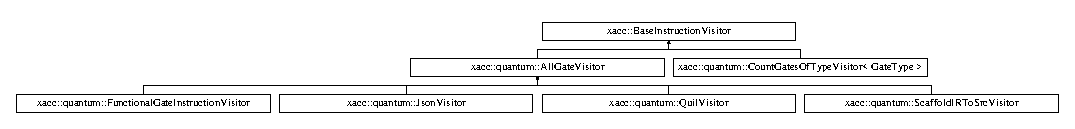
\includegraphics[height=1.288344cm]{a00018}
\end{center}
\end{figure}
\subsection*{Public Member Functions}
\begin{DoxyCompactItemize}
\item 
virtual \hyperlink{a00018_aa6f5104f5868fe1eca9be4dc4036eba4}{$\sim$\+Base\+Instruction\+Visitor} ()
\end{DoxyCompactItemize}


\subsection{Detailed Description}
The \hyperlink{a00018}{Base\+Instruction\+Visitor} is a base class for all classes that are \hyperlink{a00046}{Instruction} visitors. It basically provides a means for passing instruction visitor handles in a polymorphic manner. 

\subsection{Constructor \& Destructor Documentation}
\index{xacc\+::\+Base\+Instruction\+Visitor@{xacc\+::\+Base\+Instruction\+Visitor}!````~Base\+Instruction\+Visitor@{$\sim$\+Base\+Instruction\+Visitor}}
\index{````~Base\+Instruction\+Visitor@{$\sim$\+Base\+Instruction\+Visitor}!xacc\+::\+Base\+Instruction\+Visitor@{xacc\+::\+Base\+Instruction\+Visitor}}
\subsubsection[{\texorpdfstring{$\sim$\+Base\+Instruction\+Visitor()}{~BaseInstructionVisitor()}}]{\setlength{\rightskip}{0pt plus 5cm}virtual xacc\+::\+Base\+Instruction\+Visitor\+::$\sim$\+Base\+Instruction\+Visitor (
\begin{DoxyParamCaption}
{}
\end{DoxyParamCaption}
)\hspace{0.3cm}{\ttfamily [inline]}, {\ttfamily [virtual]}}\hypertarget{a00018_aa6f5104f5868fe1eca9be4dc4036eba4}{}\label{a00018_aa6f5104f5868fe1eca9be4dc4036eba4}
The destructor 

The documentation for this class was generated from the following file\+:\begin{DoxyCompactItemize}
\item 
Instruction\+Visitor.\+hpp\end{DoxyCompactItemize}

\hypertarget{a00019}{}\section{xacc\+:\+:quantum\+:\+:Chimera\+Graph Class Reference}
\label{a00019}\index{xacc\+::quantum\+::\+Chimera\+Graph@{xacc\+::quantum\+::\+Chimera\+Graph}}
Inheritance diagram for xacc\+:\+:quantum\+:\+:Chimera\+Graph\+:\begin{figure}[H]
\begin{center}
\leavevmode
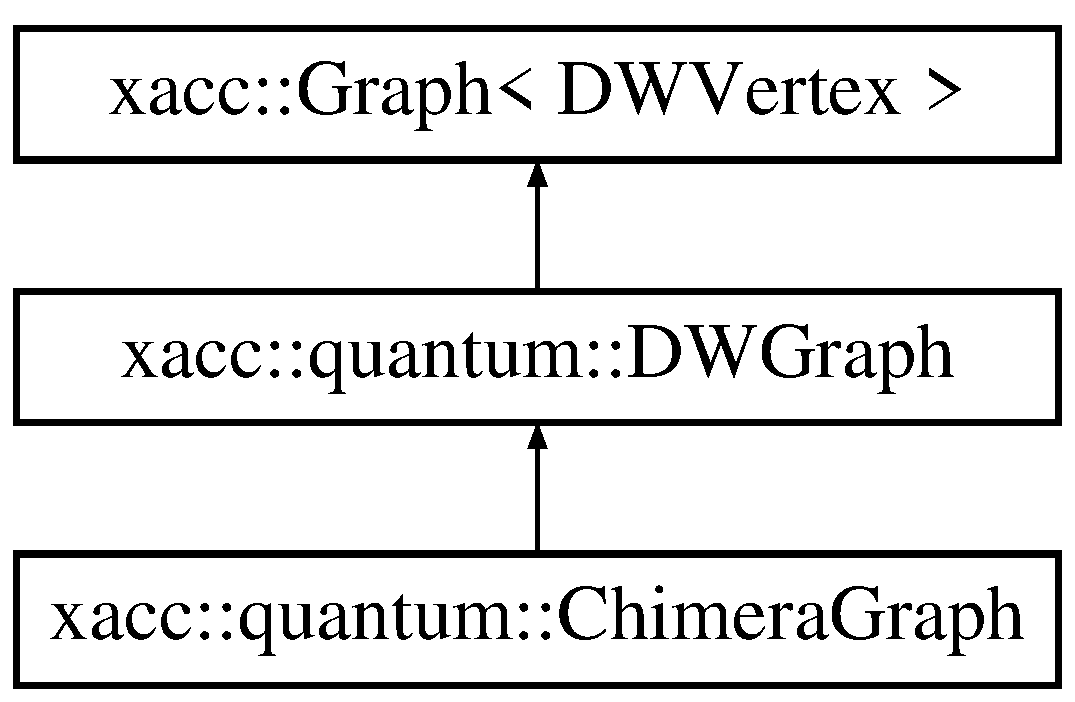
\includegraphics[height=3.000000cm]{a00019}
\end{center}
\end{figure}
\subsection*{Public Member Functions}
\begin{DoxyCompactItemize}
\item 
{\bfseries Chimera\+Graph} (int grid\+Size)\hypertarget{a00019_a64f23e464ba85d6625fe1fc2d2608052}{}\label{a00019_a64f23e464ba85d6625fe1fc2d2608052}

\end{DoxyCompactItemize}
\subsection*{Additional Inherited Members}


The documentation for this class was generated from the following file\+:\begin{DoxyCompactItemize}
\item 
D\+W\+Graph.\+hpp\end{DoxyCompactItemize}

\hypertarget{a00020}{}\section{xacc\+:\+:quantum\+:\+:Circuit\+Node Class Reference}
\label{a00020}\index{xacc\+::quantum\+::\+Circuit\+Node@{xacc\+::quantum\+::\+Circuit\+Node}}


{\ttfamily \#include $<$Gate\+Q\+I\+R.\+hpp$>$}

Inheritance diagram for xacc\+:\+:quantum\+:\+:Circuit\+Node\+:\begin{figure}[H]
\begin{center}
\leavevmode
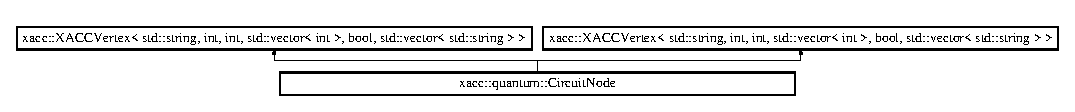
\includegraphics[height=1.060606cm]{a00020}
\end{center}
\end{figure}
\subsection*{Additional Inherited Members}


\subsection{Detailed Description}
\hyperlink{a00020}{Circuit\+Node} subclasses Q\+C\+I\+Vertex to provide the following parameters in the given order\+:

Parameters\+: Gate, Layer (ie time sequence), Gate Vertex Id, Qubit Ids that the gate acts on, enabled state, vector of parameters names 

The documentation for this class was generated from the following files\+:\begin{DoxyCompactItemize}
\item 
Gate\+Q\+I\+R.\+hpp\item 
Quantum\+Circuit.\+hpp\end{DoxyCompactItemize}

\hypertarget{a00021}{}\section{xacc\+:\+:C\+L\+I\+Parser Class Reference}
\label{a00021}\index{xacc\+::\+C\+L\+I\+Parser@{xacc\+::\+C\+L\+I\+Parser}}


{\ttfamily \#include $<$C\+L\+I\+Parser.\+hpp$>$}

\subsection*{Public Member Functions}
\begin{DoxyCompactItemize}
\item 
\hyperlink{a00021_a041f8ba22cf5e1dd1fdcdc6c9223b405}{C\+L\+I\+Parser} ()
\item 
void \hyperlink{a00021_ae6499c8c7da9b4f453757dd86028a14f}{parse} (int argc, char $\ast$$\ast$argv)
\item 
void {\bfseries add\+String\+Option} (const std\+::string key, const std\+::string description=\char`\"{}\char`\"{})\hypertarget{a00021_a793192114817fb3a9221232eab0307fd}{}\label{a00021_a793192114817fb3a9221232eab0307fd}

\end{DoxyCompactItemize}
\subsection*{Protected Attributes}
\begin{DoxyCompactItemize}
\item 
std\+::shared\+\_\+ptr$<$ options\+\_\+description $>$ \hyperlink{a00021_a0f1564966cc40c340027aecb386c4469}{xacc\+Options}
\end{DoxyCompactItemize}


\subsection{Detailed Description}
The role of the \hyperlink{a00021}{C\+L\+I\+Parser} is to parse all command line options provided to an X\+A\+C\+C-\/enabled program. It takes upon construction to available argc and argv variables from the command line, and parses them to fill the \hyperlink{a00072}{Runtime\+Options} singleton and load any X\+A\+CC \hyperlink{a00023}{Compiler} or \hyperlink{a00011}{Accelerator} plugins.

It also queries all available Option\+Providers to display all available options to the X\+A\+CC user. 

\subsection{Constructor \& Destructor Documentation}
\index{xacc\+::\+C\+L\+I\+Parser@{xacc\+::\+C\+L\+I\+Parser}!C\+L\+I\+Parser@{C\+L\+I\+Parser}}
\index{C\+L\+I\+Parser@{C\+L\+I\+Parser}!xacc\+::\+C\+L\+I\+Parser@{xacc\+::\+C\+L\+I\+Parser}}
\subsubsection[{\texorpdfstring{C\+L\+I\+Parser()}{CLIParser()}}]{\setlength{\rightskip}{0pt plus 5cm}xacc\+::\+C\+L\+I\+Parser\+::\+C\+L\+I\+Parser (
\begin{DoxyParamCaption}
{}
\end{DoxyParamCaption}
)\hspace{0.3cm}{\ttfamily [inline]}}\hypertarget{a00021_a041f8ba22cf5e1dd1fdcdc6c9223b405}{}\label{a00021_a041f8ba22cf5e1dd1fdcdc6c9223b405}
The constructor 

\subsection{Member Function Documentation}
\index{xacc\+::\+C\+L\+I\+Parser@{xacc\+::\+C\+L\+I\+Parser}!parse@{parse}}
\index{parse@{parse}!xacc\+::\+C\+L\+I\+Parser@{xacc\+::\+C\+L\+I\+Parser}}
\subsubsection[{\texorpdfstring{parse(int argc, char $\ast$$\ast$argv)}{parse(int argc, char **argv)}}]{\setlength{\rightskip}{0pt plus 5cm}void xacc\+::\+C\+L\+I\+Parser\+::parse (
\begin{DoxyParamCaption}
\item[{int}]{argc, }
\item[{char $\ast$$\ast$}]{argv}
\end{DoxyParamCaption}
)\hspace{0.3cm}{\ttfamily [inline]}}\hypertarget{a00021_ae6499c8c7da9b4f453757dd86028a14f}{}\label{a00021_ae6499c8c7da9b4f453757dd86028a14f}
Parse the command line options. Provide a Boost options\+\_\+description built up and provided by all available Options\+Providers. This method also loads all Compilers and Accelerators available in the X\+A\+C\+C\+\_\+\+I\+N\+S\+T\+A\+L\+L\+\_\+\+D\+IR. 

\subsection{Member Data Documentation}
\index{xacc\+::\+C\+L\+I\+Parser@{xacc\+::\+C\+L\+I\+Parser}!xacc\+Options@{xacc\+Options}}
\index{xacc\+Options@{xacc\+Options}!xacc\+::\+C\+L\+I\+Parser@{xacc\+::\+C\+L\+I\+Parser}}
\subsubsection[{\texorpdfstring{xacc\+Options}{xaccOptions}}]{\setlength{\rightskip}{0pt plus 5cm}std\+::shared\+\_\+ptr$<$options\+\_\+description$>$ xacc\+::\+C\+L\+I\+Parser\+::xacc\+Options\hspace{0.3cm}{\ttfamily [protected]}}\hypertarget{a00021_a0f1564966cc40c340027aecb386c4469}{}\label{a00021_a0f1564966cc40c340027aecb386c4469}
Argc, number of arguments Argv, the command line arguments 

The documentation for this class was generated from the following file\+:\begin{DoxyCompactItemize}
\item 
C\+L\+I\+Parser.\+hpp\end{DoxyCompactItemize}

\hypertarget{a00022}{}\section{xacc\+:\+:quantum\+:\+:C\+N\+OT Class Reference}
\label{a00022}\index{xacc\+::quantum\+::\+C\+N\+OT@{xacc\+::quantum\+::\+C\+N\+OT}}
Inheritance diagram for xacc\+:\+:quantum\+:\+:C\+N\+OT\+:\begin{figure}[H]
\begin{center}
\leavevmode
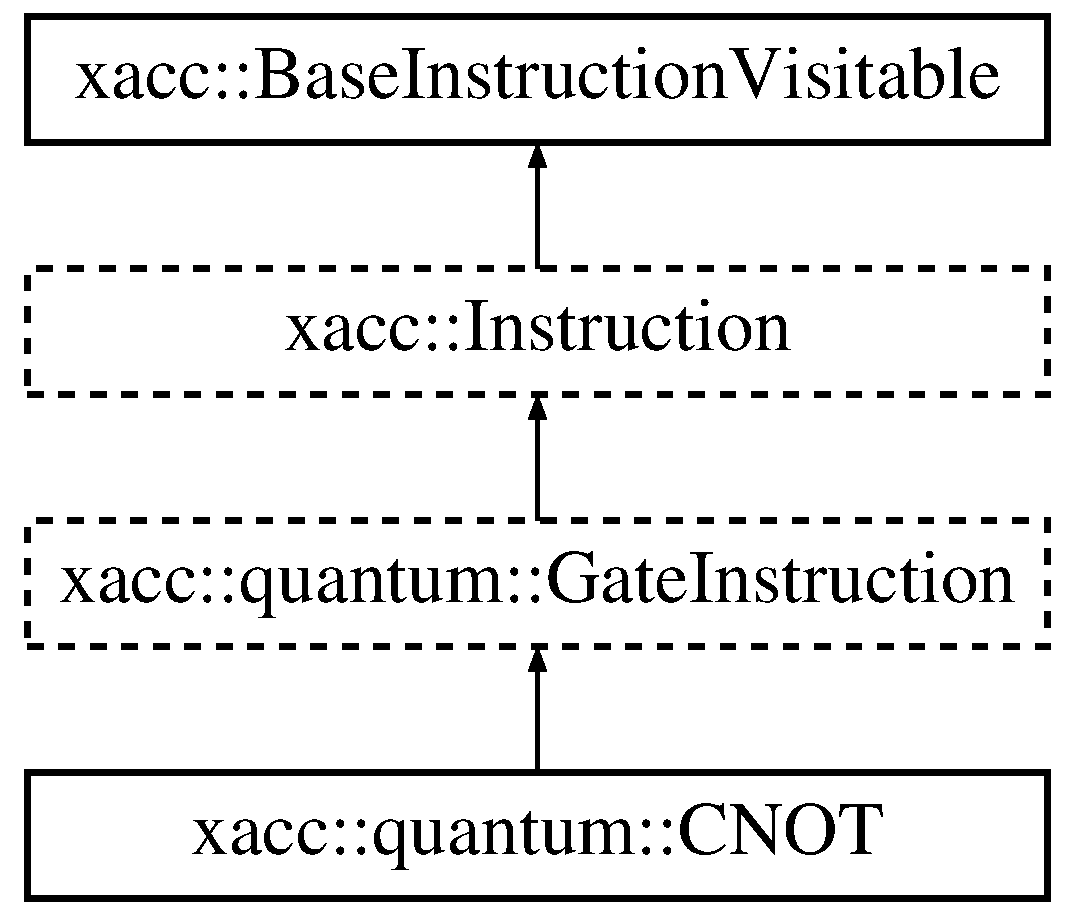
\includegraphics[height=4.000000cm]{a00022}
\end{center}
\end{figure}
\subsection*{Public Member Functions}
\begin{DoxyCompactItemize}
\item 
{\bfseries C\+N\+OT} (std\+::vector$<$ int $>$ \hyperlink{a00041_a2a56be6c2519ea65df4d06f4abae1393}{qbits})\hypertarget{a00022_ad3d460779a27affa317dd4f3a88268b3}{}\label{a00022_ad3d460779a27affa317dd4f3a88268b3}

\item 
{\bfseries C\+N\+OT} (int srcqbit, int tgtqbit)\hypertarget{a00022_a15efcb44477dde4b6151fe1776a73ddc}{}\label{a00022_a15efcb44477dde4b6151fe1776a73ddc}

\end{DoxyCompactItemize}
\subsection*{Additional Inherited Members}


The documentation for this class was generated from the following files\+:\begin{DoxyCompactItemize}
\item 
C\+N\+O\+T.\+hpp\item 
C\+N\+O\+T.\+cpp\end{DoxyCompactItemize}

\hypertarget{a00023}{}\section{xacc\+:\+:Compiler Class Reference}
\label{a00023}\index{xacc\+::\+Compiler@{xacc\+::\+Compiler}}


{\ttfamily \#include $<$Compiler.\+hpp$>$}

Inheritance diagram for xacc\+:\+:Compiler\+:\begin{figure}[H]
\begin{center}
\leavevmode
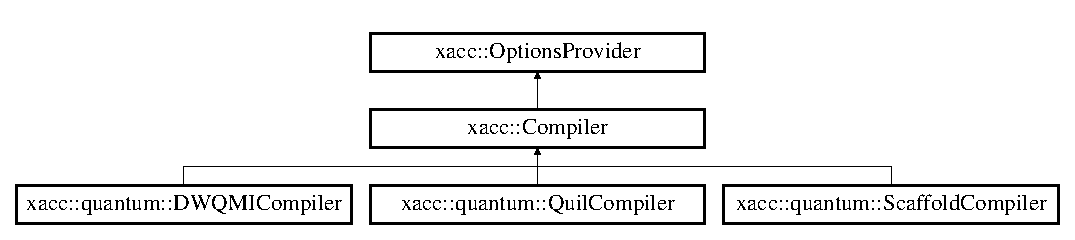
\includegraphics[height=2.772277cm]{a00023}
\end{center}
\end{figure}
\subsection*{Public Member Functions}
\begin{DoxyCompactItemize}
\item 
virtual std\+::shared\+\_\+ptr$<$ \hyperlink{a00050}{IR} $>$ \hyperlink{a00023_a546a40c95bb93af6a0c0ac48dbeaffc8}{compile} (const std\+::string \&src, std\+::shared\+\_\+ptr$<$ \hyperlink{a00011}{Accelerator} $>$ acc)=0
\item 
virtual std\+::shared\+\_\+ptr$<$ \hyperlink{a00050}{IR} $>$ \hyperlink{a00023_a9092f5f779b570c91569b59621280c04}{compile} (const std\+::string \&src)=0
\item 
virtual const std\+::string \hyperlink{a00023_aeedbe58a33fed29e4d7694ae743e25e7}{translate} (const std\+::string \&buffer\+Variable, std\+::shared\+\_\+ptr$<$ \hyperlink{a00038}{Function} $>$ function)=0
\item 
virtual const std\+::string \hyperlink{a00023_a87fca9100e6462122f5b687c3a0fb3fb}{get\+Name} ()=0
\item 
virtual std\+::shared\+\_\+ptr$<$ options\+\_\+description $>$ \hyperlink{a00023_a9f5a8965c9c2dd895016d18264ebbe92}{get\+Options} ()
\item 
virtual \hyperlink{a00023_a5d0b012687d9b44893872eaa81e47b38}{$\sim$\+Compiler} ()
\end{DoxyCompactItemize}
\subsection*{Protected Attributes}
\begin{DoxyCompactItemize}
\item 
std\+::string \hyperlink{a00023_a0ad81c816c09e5113d03cdc02165c453}{kernel\+Source}
\item 
std\+::shared\+\_\+ptr$<$ \hyperlink{a00011}{Accelerator} $>$ \hyperlink{a00023_ad4cbb467fa7e377bac6c054ffcb22b7c}{accelerator}
\end{DoxyCompactItemize}


\subsection{Detailed Description}
The \hyperlink{a00023}{Compiler} class provides an extensible interface for injecting custom compilation mechanisms into the X\+A\+CC framework. Implementations provide a compile method that takes the kernel source code string, performs compiler-\/specific compilation mechanism, and returns a valid X\+A\+CC \hyperlink{a00050}{IR} instance modeling the result of the compilation. 

\subsection{Constructor \& Destructor Documentation}
\index{xacc\+::\+Compiler@{xacc\+::\+Compiler}!````~Compiler@{$\sim$\+Compiler}}
\index{````~Compiler@{$\sim$\+Compiler}!xacc\+::\+Compiler@{xacc\+::\+Compiler}}
\subsubsection[{\texorpdfstring{$\sim$\+Compiler()}{~Compiler()}}]{\setlength{\rightskip}{0pt plus 5cm}virtual xacc\+::\+Compiler\+::$\sim$\+Compiler (
\begin{DoxyParamCaption}
{}
\end{DoxyParamCaption}
)\hspace{0.3cm}{\ttfamily [inline]}, {\ttfamily [virtual]}}\hypertarget{a00023_a5d0b012687d9b44893872eaa81e47b38}{}\label{a00023_a5d0b012687d9b44893872eaa81e47b38}
The destructor 

\subsection{Member Function Documentation}
\index{xacc\+::\+Compiler@{xacc\+::\+Compiler}!compile@{compile}}
\index{compile@{compile}!xacc\+::\+Compiler@{xacc\+::\+Compiler}}
\subsubsection[{\texorpdfstring{compile(const std\+::string \&src, std\+::shared\+\_\+ptr$<$ Accelerator $>$ acc)=0}{compile(const std::string \&src, std::shared\_ptr< Accelerator > acc)=0}}]{\setlength{\rightskip}{0pt plus 5cm}virtual std\+::shared\+\_\+ptr$<${\bf IR}$>$ xacc\+::\+Compiler\+::compile (
\begin{DoxyParamCaption}
\item[{const std\+::string \&}]{src, }
\item[{std\+::shared\+\_\+ptr$<$ {\bf Accelerator} $>$}]{acc}
\end{DoxyParamCaption}
)\hspace{0.3cm}{\ttfamily [pure virtual]}}\hypertarget{a00023_a546a40c95bb93af6a0c0ac48dbeaffc8}{}\label{a00023_a546a40c95bb93af6a0c0ac48dbeaffc8}
This method is to be implemented by derived Compilers and is in charge of executing the compilation mechanism on the provided source string. Implementations also are given access to the \hyperlink{a00011}{Accelerator} that this source code is intended for.


\begin{DoxyParams}{Parameters}
{\em src} & The kernel source string. \\
\hline
{\em acc} & The \hyperlink{a00011}{Accelerator} this code will be executed on \\
\hline
\end{DoxyParams}
\begin{DoxyReturn}{Returns}
ir Intermediate representation for provided source kernel code. 
\end{DoxyReturn}


Implemented in \hyperlink{a00034_a0df05642f1a6fd44ce7f1c0396d50c9c}{xacc\+::quantum\+::\+D\+W\+Q\+M\+I\+Compiler}, \hyperlink{a00077_a7caede75bb2304ba405966651b115543}{xacc\+::quantum\+::\+Scaffold\+Compiler}, and \hyperlink{a00062_a2421482415ca4e09963ea4ecddff8100}{xacc\+::quantum\+::\+Quil\+Compiler}.

\index{xacc\+::\+Compiler@{xacc\+::\+Compiler}!compile@{compile}}
\index{compile@{compile}!xacc\+::\+Compiler@{xacc\+::\+Compiler}}
\subsubsection[{\texorpdfstring{compile(const std\+::string \&src)=0}{compile(const std::string \&src)=0}}]{\setlength{\rightskip}{0pt plus 5cm}virtual std\+::shared\+\_\+ptr$<${\bf IR}$>$ xacc\+::\+Compiler\+::compile (
\begin{DoxyParamCaption}
\item[{const std\+::string \&}]{src}
\end{DoxyParamCaption}
)\hspace{0.3cm}{\ttfamily [pure virtual]}}\hypertarget{a00023_a9092f5f779b570c91569b59621280c04}{}\label{a00023_a9092f5f779b570c91569b59621280c04}
This method is to be implemented by derived Compilers and is in charge of executing the compilation mechanism on the provided source string. 
\begin{DoxyParams}{Parameters}
{\em src} & \\
\hline
\end{DoxyParams}
\begin{DoxyReturn}{Returns}

\end{DoxyReturn}


Implemented in \hyperlink{a00034_aa22591343b5509bf2c3a5820130ba906}{xacc\+::quantum\+::\+D\+W\+Q\+M\+I\+Compiler}, \hyperlink{a00077_a3736ecc229fe6acdd4c991e85d7a1f08}{xacc\+::quantum\+::\+Scaffold\+Compiler}, and \hyperlink{a00062_adf4d321ecb0df3fa7728999f941c83b2}{xacc\+::quantum\+::\+Quil\+Compiler}.

\index{xacc\+::\+Compiler@{xacc\+::\+Compiler}!get\+Name@{get\+Name}}
\index{get\+Name@{get\+Name}!xacc\+::\+Compiler@{xacc\+::\+Compiler}}
\subsubsection[{\texorpdfstring{get\+Name()=0}{getName()=0}}]{\setlength{\rightskip}{0pt plus 5cm}virtual const std\+::string xacc\+::\+Compiler\+::get\+Name (
\begin{DoxyParamCaption}
{}
\end{DoxyParamCaption}
)\hspace{0.3cm}{\ttfamily [pure virtual]}}\hypertarget{a00023_a87fca9100e6462122f5b687c3a0fb3fb}{}\label{a00023_a87fca9100e6462122f5b687c3a0fb3fb}
Return the name of this \hyperlink{a00023}{Compiler} \begin{DoxyReturn}{Returns}
name \hyperlink{a00023}{Compiler} name 
\end{DoxyReturn}


Implemented in \hyperlink{a00034_aed42de96f8e0dd94b6de183f28aee419}{xacc\+::quantum\+::\+D\+W\+Q\+M\+I\+Compiler}, \hyperlink{a00077_a3f537054a3924a1d14f4ceb0f0181161}{xacc\+::quantum\+::\+Scaffold\+Compiler}, and \hyperlink{a00062_ae7d52140b6dd52730edc6e38ae48f437}{xacc\+::quantum\+::\+Quil\+Compiler}.

\index{xacc\+::\+Compiler@{xacc\+::\+Compiler}!get\+Options@{get\+Options}}
\index{get\+Options@{get\+Options}!xacc\+::\+Compiler@{xacc\+::\+Compiler}}
\subsubsection[{\texorpdfstring{get\+Options()}{getOptions()}}]{\setlength{\rightskip}{0pt plus 5cm}virtual std\+::shared\+\_\+ptr$<$options\+\_\+description$>$ xacc\+::\+Compiler\+::get\+Options (
\begin{DoxyParamCaption}
{}
\end{DoxyParamCaption}
)\hspace{0.3cm}{\ttfamily [inline]}, {\ttfamily [virtual]}}\hypertarget{a00023_a9f5a8965c9c2dd895016d18264ebbe92}{}\label{a00023_a9f5a8965c9c2dd895016d18264ebbe92}
Return an empty options\+\_\+description, this is for subclasses to implement. 

Implements \hyperlink{a00056_a6d150954f852109bfe2c1ae90222926f}{xacc\+::\+Options\+Provider}.



Reimplemented in \hyperlink{a00034_a0851334cc33b5b1da2694150a0a1a43c}{xacc\+::quantum\+::\+D\+W\+Q\+M\+I\+Compiler}.

\index{xacc\+::\+Compiler@{xacc\+::\+Compiler}!translate@{translate}}
\index{translate@{translate}!xacc\+::\+Compiler@{xacc\+::\+Compiler}}
\subsubsection[{\texorpdfstring{translate(const std\+::string \&buffer\+Variable, std\+::shared\+\_\+ptr$<$ Function $>$ function)=0}{translate(const std::string \&bufferVariable, std::shared\_ptr< Function > function)=0}}]{\setlength{\rightskip}{0pt plus 5cm}virtual const std\+::string xacc\+::\+Compiler\+::translate (
\begin{DoxyParamCaption}
\item[{const std\+::string \&}]{buffer\+Variable, }
\item[{std\+::shared\+\_\+ptr$<$ {\bf Function} $>$}]{function}
\end{DoxyParamCaption}
)\hspace{0.3cm}{\ttfamily [pure virtual]}}\hypertarget{a00023_aeedbe58a33fed29e4d7694ae743e25e7}{}\label{a00023_aeedbe58a33fed29e4d7694ae743e25e7}
This method is to be implemented by derived Compilers and is in charge of taking the provided \hyperlink{a00038}{Function} \hyperlink{a00050}{IR} and converting it to source code in this \hyperlink{a00023}{Compiler}\textquotesingle{}s language.


\begin{DoxyParams}{Parameters}
{\em function} & The X\+A\+CC \hyperlink{a00050}{IR} \hyperlink{a00038}{Function} to translate \\
\hline
\end{DoxyParams}
\begin{DoxyReturn}{Returns}
src The source code as a string 
\end{DoxyReturn}


Implemented in \hyperlink{a00034_a56a345539665099329209b3b5f6810c9}{xacc\+::quantum\+::\+D\+W\+Q\+M\+I\+Compiler}, \hyperlink{a00062_a66ca00bbb1f30e7bc6dd86b1e267b93b}{xacc\+::quantum\+::\+Quil\+Compiler}, and \hyperlink{a00077_ac7ca2941e987ba579c6f50cfbd7fb0dc}{xacc\+::quantum\+::\+Scaffold\+Compiler}.



\subsection{Member Data Documentation}
\index{xacc\+::\+Compiler@{xacc\+::\+Compiler}!accelerator@{accelerator}}
\index{accelerator@{accelerator}!xacc\+::\+Compiler@{xacc\+::\+Compiler}}
\subsubsection[{\texorpdfstring{accelerator}{accelerator}}]{\setlength{\rightskip}{0pt plus 5cm}std\+::shared\+\_\+ptr$<${\bf Accelerator}$>$ xacc\+::\+Compiler\+::accelerator\hspace{0.3cm}{\ttfamily [protected]}}\hypertarget{a00023_ad4cbb467fa7e377bac6c054ffcb22b7c}{}\label{a00023_ad4cbb467fa7e377bac6c054ffcb22b7c}
Reference to the \hyperlink{a00011}{Accelerator} that this compiler is targeting. \index{xacc\+::\+Compiler@{xacc\+::\+Compiler}!kernel\+Source@{kernel\+Source}}
\index{kernel\+Source@{kernel\+Source}!xacc\+::\+Compiler@{xacc\+::\+Compiler}}
\subsubsection[{\texorpdfstring{kernel\+Source}{kernelSource}}]{\setlength{\rightskip}{0pt plus 5cm}std\+::string xacc\+::\+Compiler\+::kernel\+Source\hspace{0.3cm}{\ttfamily [protected]}}\hypertarget{a00023_a0ad81c816c09e5113d03cdc02165c453}{}\label{a00023_a0ad81c816c09e5113d03cdc02165c453}
Reference to the provided kernel source code string 

The documentation for this class was generated from the following file\+:\begin{DoxyCompactItemize}
\item 
Compiler.\+hpp\end{DoxyCompactItemize}

\hypertarget{a00024}{}\section{xacc\+:\+:quantum\+:\+:Complete\+Graph Class Reference}
\label{a00024}\index{xacc\+::quantum\+::\+Complete\+Graph@{xacc\+::quantum\+::\+Complete\+Graph}}
Inheritance diagram for xacc\+:\+:quantum\+:\+:Complete\+Graph\+:\begin{figure}[H]
\begin{center}
\leavevmode
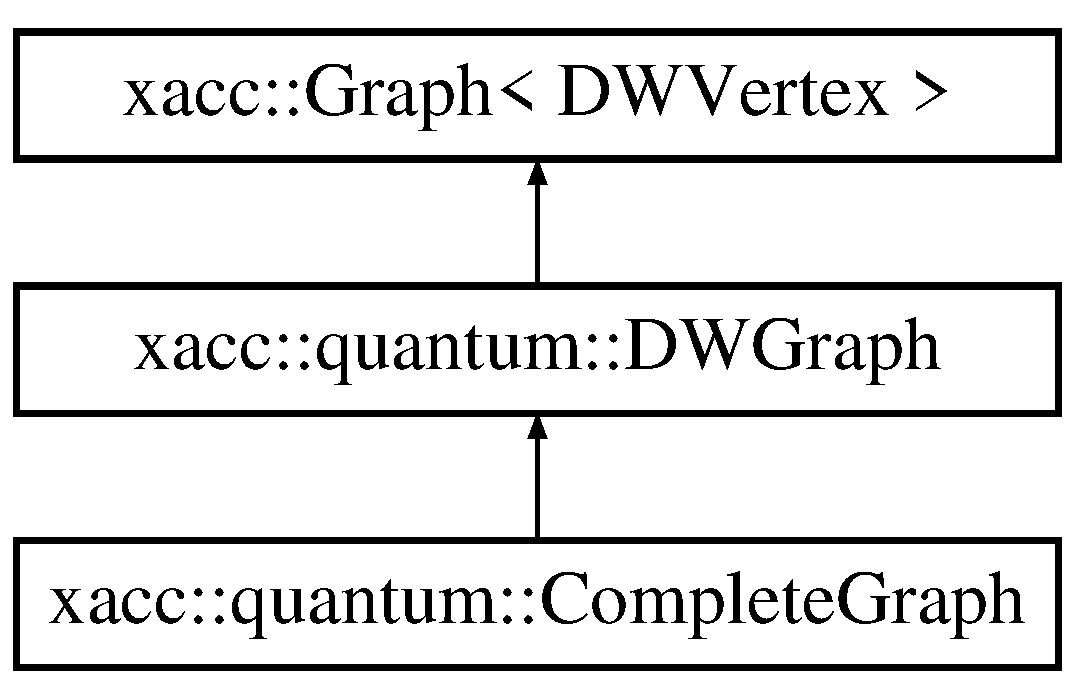
\includegraphics[height=3.000000cm]{a00024}
\end{center}
\end{figure}
\subsection*{Public Member Functions}
\begin{DoxyCompactItemize}
\item 
{\bfseries Complete\+Graph} (int n\+Vertices)\hypertarget{a00024_a70eeb65709e217e61bb0066365579c39}{}\label{a00024_a70eeb65709e217e61bb0066365579c39}

\end{DoxyCompactItemize}
\subsection*{Additional Inherited Members}


The documentation for this class was generated from the following file\+:\begin{DoxyCompactItemize}
\item 
D\+W\+Graph.\+hpp\end{DoxyCompactItemize}

\hypertarget{a00025}{}\section{xacc\+:\+:quantum\+:\+:Conditional\+Function Class Reference}
\label{a00025}\index{xacc\+::quantum\+::\+Conditional\+Function@{xacc\+::quantum\+::\+Conditional\+Function}}
Inheritance diagram for xacc\+:\+:quantum\+:\+:Conditional\+Function\+:\begin{figure}[H]
\begin{center}
\leavevmode
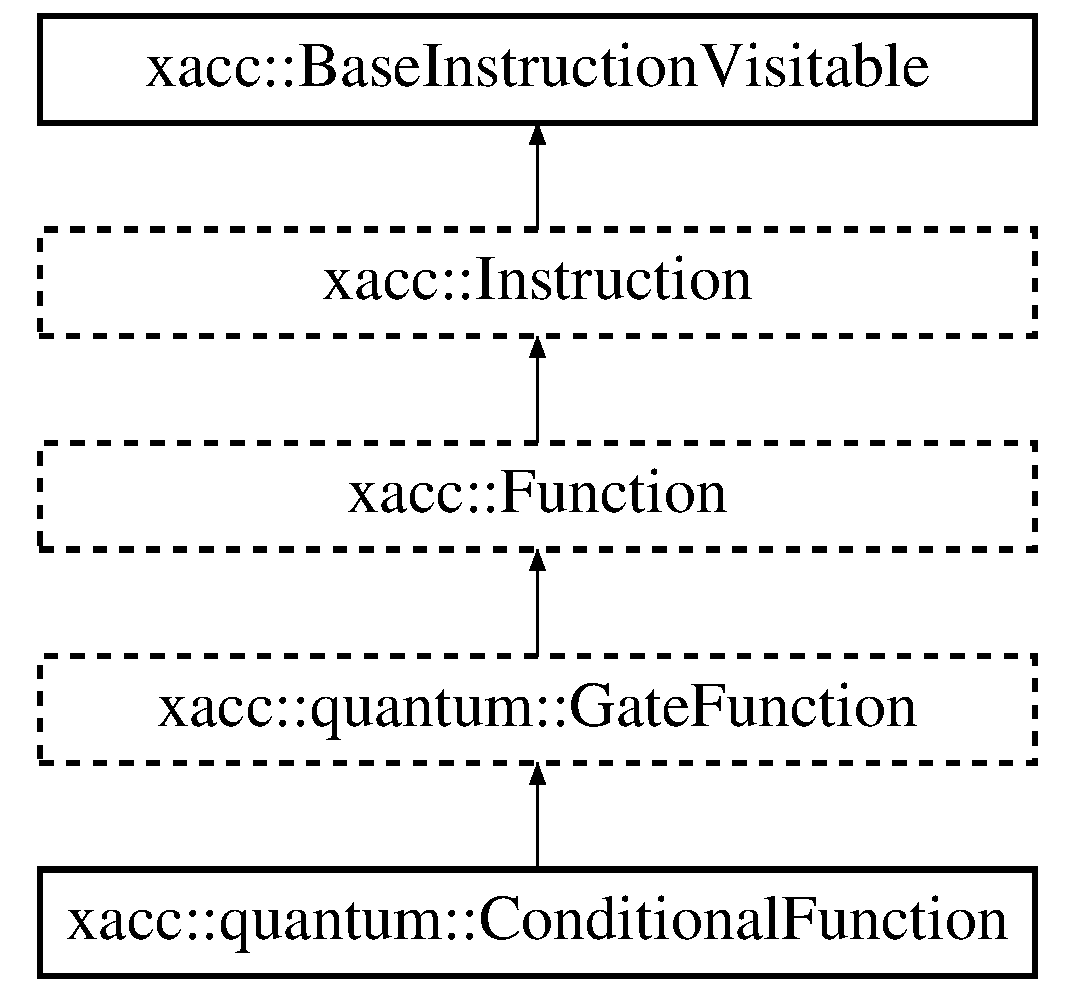
\includegraphics[height=5.000000cm]{a00025}
\end{center}
\end{figure}
\subsection*{Public Member Functions}
\begin{DoxyCompactItemize}
\item 
{\bfseries Conditional\+Function} (int qbit)\hypertarget{a00025_aa28610a08ae04d62ccdd8359433100c3}{}\label{a00025_aa28610a08ae04d62ccdd8359433100c3}

\item 
virtual void \hyperlink{a00025_a6aedad20f96390880efdc0a476b3273f}{add\+Instruction} (Inst\+Ptr instruction)
\item 
const int {\bfseries get\+Conditional\+Qubit} ()\hypertarget{a00025_a804317333b6677a041a3071b5108c0df}{}\label{a00025_a804317333b6677a041a3071b5108c0df}

\item 
void {\bfseries evaluate} (const int acc\+Bit\+State)\hypertarget{a00025_a709c236a5beb62d9a3bd5265196fb6c9}{}\label{a00025_a709c236a5beb62d9a3bd5265196fb6c9}

\item 
virtual const std\+::string \hyperlink{a00025_aca7a5f849fece6fc28a904efee9a3370}{to\+String} (const std\+::string \&buffer\+Var\+Name)
\end{DoxyCompactItemize}
\subsection*{Protected Attributes}
\begin{DoxyCompactItemize}
\item 
int {\bfseries qbit\+Idx}\hypertarget{a00025_a0310536801417c0eded28a4dea1efa44}{}\label{a00025_a0310536801417c0eded28a4dea1efa44}

\end{DoxyCompactItemize}
\subsection*{Additional Inherited Members}


\subsection{Member Function Documentation}
\index{xacc\+::quantum\+::\+Conditional\+Function@{xacc\+::quantum\+::\+Conditional\+Function}!add\+Instruction@{add\+Instruction}}
\index{add\+Instruction@{add\+Instruction}!xacc\+::quantum\+::\+Conditional\+Function@{xacc\+::quantum\+::\+Conditional\+Function}}
\subsubsection[{\texorpdfstring{add\+Instruction(\+Inst\+Ptr instruction)}{addInstruction(InstPtr instruction)}}]{\setlength{\rightskip}{0pt plus 5cm}void xacc\+::quantum\+::\+Conditional\+Function\+::add\+Instruction (
\begin{DoxyParamCaption}
\item[{Inst\+Ptr}]{instruction}
\end{DoxyParamCaption}
)\hspace{0.3cm}{\ttfamily [virtual]}}\hypertarget{a00025_a6aedad20f96390880efdc0a476b3273f}{}\label{a00025_a6aedad20f96390880efdc0a476b3273f}
Add an instruction to this quantum intermediate representation.


\begin{DoxyParams}{Parameters}
{\em instruction} & \\
\hline
\end{DoxyParams}


Reimplemented from \hyperlink{a00040_a892fb69a10f0a7cb5abdab4cca61b80a}{xacc\+::quantum\+::\+Gate\+Function}.

\index{xacc\+::quantum\+::\+Conditional\+Function@{xacc\+::quantum\+::\+Conditional\+Function}!to\+String@{to\+String}}
\index{to\+String@{to\+String}!xacc\+::quantum\+::\+Conditional\+Function@{xacc\+::quantum\+::\+Conditional\+Function}}
\subsubsection[{\texorpdfstring{to\+String(const std\+::string \&buffer\+Var\+Name)}{toString(const std::string \&bufferVarName)}}]{\setlength{\rightskip}{0pt plus 5cm}const std\+::string xacc\+::quantum\+::\+Conditional\+Function\+::to\+String (
\begin{DoxyParamCaption}
\item[{const std\+::string \&}]{buffer\+Var\+Name}
\end{DoxyParamCaption}
)\hspace{0.3cm}{\ttfamily [virtual]}}\hypertarget{a00025_aca7a5f849fece6fc28a904efee9a3370}{}\label{a00025_aca7a5f849fece6fc28a904efee9a3370}
Return an assembly-\/like string representation for this function . 
\begin{DoxyParams}{Parameters}
{\em buffer\+Var\+Name} & \\
\hline
\end{DoxyParams}
\begin{DoxyReturn}{Returns}

\end{DoxyReturn}


Reimplemented from \hyperlink{a00040_aa1950776ae84bad2d0795a0441f910e7}{xacc\+::quantum\+::\+Gate\+Function}.



The documentation for this class was generated from the following files\+:\begin{DoxyCompactItemize}
\item 
Conditional\+Function.\+hpp\item 
Conditional\+Function.\+cpp\end{DoxyCompactItemize}

\hypertarget{a00026}{}\section{xacc\+:\+:quantum\+:\+:Count\+Gates\+Of\+Type\+Visitor$<$ Gate\+Type $>$ Class Template Reference}
\label{a00026}\index{xacc\+::quantum\+::\+Count\+Gates\+Of\+Type\+Visitor$<$ Gate\+Type $>$@{xacc\+::quantum\+::\+Count\+Gates\+Of\+Type\+Visitor$<$ Gate\+Type $>$}}
Inheritance diagram for xacc\+:\+:quantum\+:\+:Count\+Gates\+Of\+Type\+Visitor$<$ Gate\+Type $>$\+:\begin{figure}[H]
\begin{center}
\leavevmode
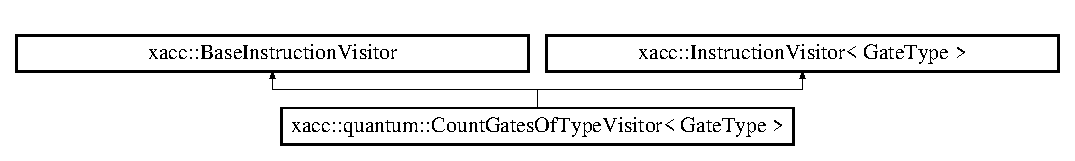
\includegraphics[height=1.717791cm]{a00026}
\end{center}
\end{figure}
\subsection*{Public Member Functions}
\begin{DoxyCompactItemize}
\item 
{\bfseries Count\+Gates\+Of\+Type\+Visitor} (std\+::shared\+\_\+ptr$<$ \hyperlink{a00038}{Function} $>$ f)\hypertarget{a00026_a4c2507e3ee4fe51e7ff4501bf5569cfc}{}\label{a00026_a4c2507e3ee4fe51e7ff4501bf5569cfc}

\item 
virtual void \hyperlink{a00026_a9c40e6cb4b74e2d6714c531ffc3b2909}{visit} (Gate\+Type \&gate)
\item 
int {\bfseries count\+Gates} ()\hypertarget{a00026_a8a1a17ed50cd6727c2eb07976f886389}{}\label{a00026_a8a1a17ed50cd6727c2eb07976f886389}

\end{DoxyCompactItemize}
\subsection*{Protected Attributes}
\begin{DoxyCompactItemize}
\item 
int {\bfseries count} = 0\hypertarget{a00026_ae3d8ae4c40c1552ee68aa6e5002e42bd}{}\label{a00026_ae3d8ae4c40c1552ee68aa6e5002e42bd}

\item 
std\+::shared\+\_\+ptr$<$ \hyperlink{a00038}{Function} $>$ {\bfseries function}\hypertarget{a00026_a202ab6e0e365af735da706fe972333e7}{}\label{a00026_a202ab6e0e365af735da706fe972333e7}

\end{DoxyCompactItemize}


\subsection{Member Function Documentation}
\index{xacc\+::quantum\+::\+Count\+Gates\+Of\+Type\+Visitor@{xacc\+::quantum\+::\+Count\+Gates\+Of\+Type\+Visitor}!visit@{visit}}
\index{visit@{visit}!xacc\+::quantum\+::\+Count\+Gates\+Of\+Type\+Visitor@{xacc\+::quantum\+::\+Count\+Gates\+Of\+Type\+Visitor}}
\subsubsection[{\texorpdfstring{visit(\+Gate\+Type \&gate)}{visit(GateType \&gate)}}]{\setlength{\rightskip}{0pt plus 5cm}template$<$typename Gate\+Type $>$ virtual void {\bf xacc\+::quantum\+::\+Count\+Gates\+Of\+Type\+Visitor}$<$ Gate\+Type $>$\+::visit (
\begin{DoxyParamCaption}
\item[{Gate\+Type \&}]{}
\end{DoxyParamCaption}
)\hspace{0.3cm}{\ttfamily [inline]}, {\ttfamily [virtual]}}\hypertarget{a00026_a9c40e6cb4b74e2d6714c531ffc3b2909}{}\label{a00026_a9c40e6cb4b74e2d6714c531ffc3b2909}
This method should be implemented by subclasses to perform Visitor-\/specific behavior on the given instance of the template parameter T. 

Implements \hyperlink{a00048_af0fead298f5bfbb8e6680433063e2c4b}{xacc\+::\+Instruction\+Visitor$<$ Gate\+Type $>$}.



The documentation for this class was generated from the following file\+:\begin{DoxyCompactItemize}
\item 
Count\+Gates\+Of\+Type\+Visitor.\+hpp\end{DoxyCompactItemize}

\hypertarget{a00027}{}\section{xacc\+:\+:quantum\+:\+:C\+Phase Class Reference}
\label{a00027}\index{xacc\+::quantum\+::\+C\+Phase@{xacc\+::quantum\+::\+C\+Phase}}
Inheritance diagram for xacc\+:\+:quantum\+:\+:C\+Phase\+:\begin{figure}[H]
\begin{center}
\leavevmode
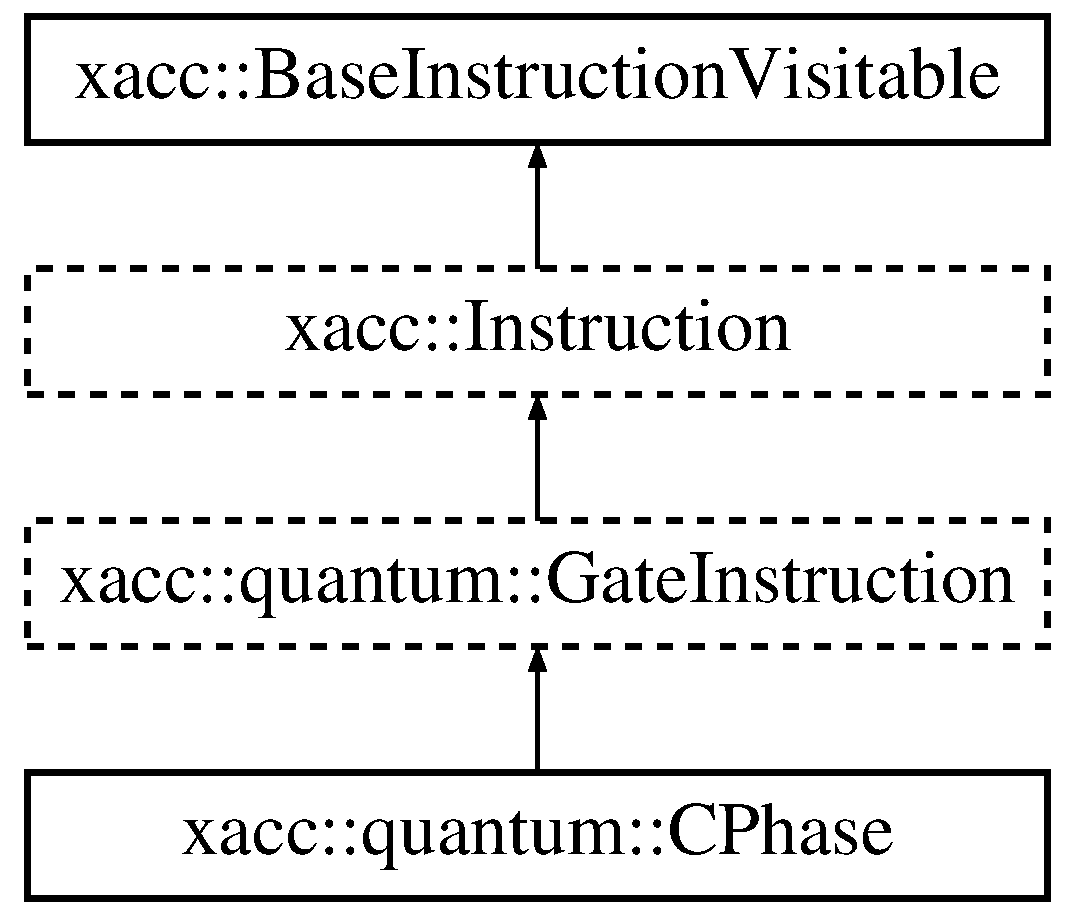
\includegraphics[height=4.000000cm]{a00027}
\end{center}
\end{figure}
\subsection*{Public Member Functions}
\begin{DoxyCompactItemize}
\item 
{\bfseries C\+Phase} (std\+::vector$<$ int $>$ \hyperlink{a00041_a2a56be6c2519ea65df4d06f4abae1393}{qbits})\hypertarget{a00027_a5899f838bc4b892d179f51fcf0ac4cc8}{}\label{a00027_a5899f838bc4b892d179f51fcf0ac4cc8}

\item 
{\bfseries C\+Phase} (int control\+Qubit, int target\+Qubit, double theta)\hypertarget{a00027_af642f499455f0065279a1e1d178c818f}{}\label{a00027_af642f499455f0065279a1e1d178c818f}

\end{DoxyCompactItemize}
\subsection*{Additional Inherited Members}


The documentation for this class was generated from the following files\+:\begin{DoxyCompactItemize}
\item 
C\+Phase.\+hpp\item 
C\+Phase.\+cpp\end{DoxyCompactItemize}

\hypertarget{a00028}{}\section{xacc\+:\+:Default\+Edge Struct Reference}
\label{a00028}\index{xacc\+::\+Default\+Edge@{xacc\+::\+Default\+Edge}}


{\ttfamily \#include $<$Graph.\+hpp$>$}

\subsection*{Public Attributes}
\begin{DoxyCompactItemize}
\item 
double {\bfseries weight} = 0.\+0\hypertarget{a00028_a71d942e4d65d04a2e611759121845e71}{}\label{a00028_a71d942e4d65d04a2e611759121845e71}

\end{DoxyCompactItemize}


\subsection{Detailed Description}
For now, we only allow Edges with weight property. 

The documentation for this struct was generated from the following file\+:\begin{DoxyCompactItemize}
\item 
Graph.\+hpp\end{DoxyCompactItemize}

\hypertarget{a00029}{}\section{xacc\+:\+:quantum\+:\+:D\+W\+Accelerator Class Reference}
\label{a00029}\index{xacc\+::quantum\+::\+D\+W\+Accelerator@{xacc\+::quantum\+::\+D\+W\+Accelerator}}


{\ttfamily \#include $<$D\+W\+Accelerator.\+hpp$>$}

Inheritance diagram for xacc\+:\+:quantum\+:\+:D\+W\+Accelerator\+:\begin{figure}[H]
\begin{center}
\leavevmode
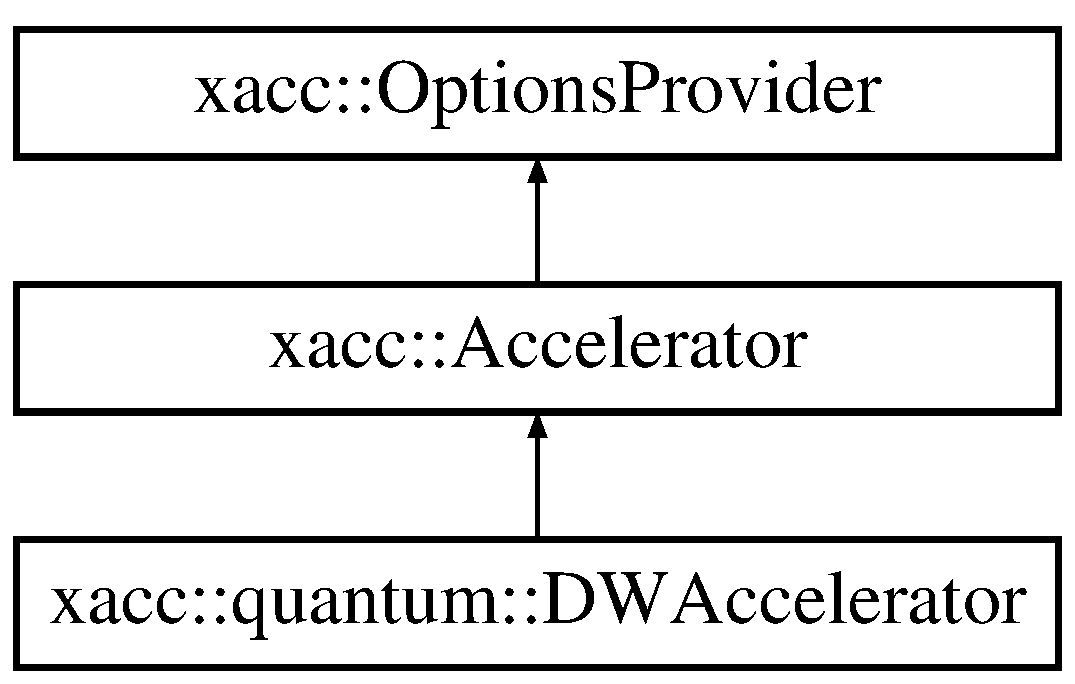
\includegraphics[height=3.000000cm]{a00029}
\end{center}
\end{figure}
\subsection*{Public Member Functions}
\begin{DoxyCompactItemize}
\item 
\hyperlink{a00029_ad6924d7e9812df5e4676109352ee74a7}{D\+W\+Accelerator} ()
\item 
std\+::shared\+\_\+ptr$<$ \hyperlink{a00013}{Accelerator\+Buffer} $>$ \hyperlink{a00029_a718d7cb51a35e694d960385e1ea2f99f}{create\+Buffer} (const std\+::string \&var\+Id, const int size)
\item 
virtual bool \hyperlink{a00029_a4c2ee30212a919d8ddf7f9555df25195}{is\+Valid\+Buffer\+Size} (const int N\+Bits)
\item 
virtual std\+::shared\+\_\+ptr$<$ \hyperlink{a00043}{Accelerator\+Graph} $>$ \hyperlink{a00029_a006afa60749790681fc76beddc254926}{get\+Accelerator\+Connectivity} ()
\item 
virtual void \hyperlink{a00029_aa8d770acb2708b3ee1cd1f21bd0cc668}{execute} (std\+::shared\+\_\+ptr$<$ \hyperlink{a00013}{Accelerator\+Buffer} $>$ buffer, const std\+::shared\+\_\+ptr$<$ \hyperlink{a00038}{xacc\+::\+Function} $>$ kernel)
\item 
virtual Accelerator\+Type \hyperlink{a00029_abe50e427b4bec0460cc238405cb569f9}{get\+Type} ()
\item 
virtual std\+::vector$<$ \hyperlink{a00051}{xacc\+::\+I\+R\+Transformation} $>$ \hyperlink{a00029_a89da20bd079a22d6581ea2da2293b973}{get\+I\+R\+Transformations} ()
\item 
virtual std\+::shared\+\_\+ptr$<$ options\+\_\+description $>$ \hyperlink{a00029_a09926db9f99706307ae6ce5b56845bca}{get\+Options} ()
\item 
virtual void \hyperlink{a00029_acaefd5747409f31cf5c3e42d98475ce2}{initialize} ()
\item 
virtual std\+::shared\+\_\+ptr$<$ \hyperlink{a00013}{Accelerator\+Buffer} $>$ \hyperlink{a00029_add60637a4b3c055e7f2ffa3bf8e320ac}{create\+Buffer} (const std\+::string \&var\+Id)
\item 
virtual \hyperlink{a00029_ad06f92a271d445c2a1ff8364faa3617b}{$\sim$\+D\+W\+Accelerator} ()
\end{DoxyCompactItemize}
\subsection*{Static Public Member Functions}
\begin{DoxyCompactItemize}
\item 
static void \hyperlink{a00029_aece856713312dd2c882eee12392b04fa}{register\+Accelerator} ()
\end{DoxyCompactItemize}
\subsection*{Protected Attributes}
\begin{DoxyCompactItemize}
\item 
std\+::string \hyperlink{a00029_a6b9ca421d7efeed09ff9acb9f77d9dd8}{api\+Key}
\item 
std\+::string \hyperlink{a00029_a934db80f3cf6aa68158a66bc053c0c27}{url}
\item 
std\+::map$<$ std\+::string, std\+::string $>$ \hyperlink{a00029_a031df31e3ff84f33ea9a76bfc0f9277c}{headers}
\item 
std\+::map$<$ std\+::string, \hyperlink{a00035}{D\+W\+Solver} $>$ \hyperlink{a00029_ac19954e3df9e77184717c9be8a2ed4c5}{available\+Solvers}
\end{DoxyCompactItemize}
\subsection*{Additional Inherited Members}


\subsection{Detailed Description}
The \hyperlink{a00029}{D\+W\+Accelerator} is an X\+A\+CC \hyperlink{a00011}{Accelerator} that takes D-\/\+Wave \hyperlink{a00050}{IR} and executes the quantum machine instructions via remote H\+T\+TP invocations. 

\subsection{Constructor \& Destructor Documentation}
\index{xacc\+::quantum\+::\+D\+W\+Accelerator@{xacc\+::quantum\+::\+D\+W\+Accelerator}!D\+W\+Accelerator@{D\+W\+Accelerator}}
\index{D\+W\+Accelerator@{D\+W\+Accelerator}!xacc\+::quantum\+::\+D\+W\+Accelerator@{xacc\+::quantum\+::\+D\+W\+Accelerator}}
\subsubsection[{\texorpdfstring{D\+W\+Accelerator()}{DWAccelerator()}}]{\setlength{\rightskip}{0pt plus 5cm}xacc\+::quantum\+::\+D\+W\+Accelerator\+::\+D\+W\+Accelerator (
\begin{DoxyParamCaption}
{}
\end{DoxyParamCaption}
)\hspace{0.3cm}{\ttfamily [inline]}}\hypertarget{a00029_ad6924d7e9812df5e4676109352ee74a7}{}\label{a00029_ad6924d7e9812df5e4676109352ee74a7}
The constructor \index{xacc\+::quantum\+::\+D\+W\+Accelerator@{xacc\+::quantum\+::\+D\+W\+Accelerator}!````~D\+W\+Accelerator@{$\sim$\+D\+W\+Accelerator}}
\index{````~D\+W\+Accelerator@{$\sim$\+D\+W\+Accelerator}!xacc\+::quantum\+::\+D\+W\+Accelerator@{xacc\+::quantum\+::\+D\+W\+Accelerator}}
\subsubsection[{\texorpdfstring{$\sim$\+D\+W\+Accelerator()}{~DWAccelerator()}}]{\setlength{\rightskip}{0pt plus 5cm}virtual xacc\+::quantum\+::\+D\+W\+Accelerator\+::$\sim$\+D\+W\+Accelerator (
\begin{DoxyParamCaption}
{}
\end{DoxyParamCaption}
)\hspace{0.3cm}{\ttfamily [inline]}, {\ttfamily [virtual]}}\hypertarget{a00029_ad06f92a271d445c2a1ff8364faa3617b}{}\label{a00029_ad06f92a271d445c2a1ff8364faa3617b}
The destructor 

\subsection{Member Function Documentation}
\index{xacc\+::quantum\+::\+D\+W\+Accelerator@{xacc\+::quantum\+::\+D\+W\+Accelerator}!create\+Buffer@{create\+Buffer}}
\index{create\+Buffer@{create\+Buffer}!xacc\+::quantum\+::\+D\+W\+Accelerator@{xacc\+::quantum\+::\+D\+W\+Accelerator}}
\subsubsection[{\texorpdfstring{create\+Buffer(const std\+::string \&var\+Id, const int size)}{createBuffer(const std::string \&varId, const int size)}}]{\setlength{\rightskip}{0pt plus 5cm}std\+::shared\+\_\+ptr$<$ {\bf Accelerator\+Buffer} $>$ xacc\+::quantum\+::\+D\+W\+Accelerator\+::create\+Buffer (
\begin{DoxyParamCaption}
\item[{const std\+::string \&}]{var\+Id, }
\item[{const int}]{size}
\end{DoxyParamCaption}
)\hspace{0.3cm}{\ttfamily [virtual]}}\hypertarget{a00029_a718d7cb51a35e694d960385e1ea2f99f}{}\label{a00029_a718d7cb51a35e694d960385e1ea2f99f}
Create, store, and return an \hyperlink{a00013}{Accelerator\+Buffer} with the given variable id string and of the given number of bits. The string id serves as a unique identifier for future lookups and reuse of the \hyperlink{a00013}{Accelerator\+Buffer}.


\begin{DoxyParams}{Parameters}
{\em var\+Id} & \\
\hline
{\em size} & \\
\hline
\end{DoxyParams}
\begin{DoxyReturn}{Returns}

\end{DoxyReturn}


Implements \hyperlink{a00011_a064a2dbd58338364115c260267806945}{xacc\+::\+Accelerator}.

\index{xacc\+::quantum\+::\+D\+W\+Accelerator@{xacc\+::quantum\+::\+D\+W\+Accelerator}!create\+Buffer@{create\+Buffer}}
\index{create\+Buffer@{create\+Buffer}!xacc\+::quantum\+::\+D\+W\+Accelerator@{xacc\+::quantum\+::\+D\+W\+Accelerator}}
\subsubsection[{\texorpdfstring{create\+Buffer(const std\+::string \&var\+Id)}{createBuffer(const std::string \&varId)}}]{\setlength{\rightskip}{0pt plus 5cm}virtual std\+::shared\+\_\+ptr$<${\bf Accelerator\+Buffer}$>$ xacc\+::quantum\+::\+D\+W\+Accelerator\+::create\+Buffer (
\begin{DoxyParamCaption}
\item[{const std\+::string \&}]{var\+Id}
\end{DoxyParamCaption}
)\hspace{0.3cm}{\ttfamily [inline]}, {\ttfamily [virtual]}}\hypertarget{a00029_add60637a4b3c055e7f2ffa3bf8e320ac}{}\label{a00029_add60637a4b3c055e7f2ffa3bf8e320ac}
Create and return an \hyperlink{a00016}{A\+Q\+C\+Accelerator\+Buffer} of size dictated by the current solver being used.


\begin{DoxyParams}{Parameters}
{\em var\+Id} & The name of this buffer \\
\hline
\end{DoxyParams}
\begin{DoxyReturn}{Returns}
buffer The \hyperlink{a00013}{Accelerator\+Buffer} 
\end{DoxyReturn}


Implements \hyperlink{a00011_aab5046e8d83ab390302e0f49533e95fc}{xacc\+::\+Accelerator}.

\index{xacc\+::quantum\+::\+D\+W\+Accelerator@{xacc\+::quantum\+::\+D\+W\+Accelerator}!execute@{execute}}
\index{execute@{execute}!xacc\+::quantum\+::\+D\+W\+Accelerator@{xacc\+::quantum\+::\+D\+W\+Accelerator}}
\subsubsection[{\texorpdfstring{execute(std\+::shared\+\_\+ptr$<$ Accelerator\+Buffer $>$ buffer, const std\+::shared\+\_\+ptr$<$ xacc\+::\+Function $>$ kernel)}{execute(std::shared\_ptr< AcceleratorBuffer > buffer, const std::shared\_ptr< xacc::Function > kernel)}}]{\setlength{\rightskip}{0pt plus 5cm}void xacc\+::quantum\+::\+D\+W\+Accelerator\+::execute (
\begin{DoxyParamCaption}
\item[{std\+::shared\+\_\+ptr$<$ {\bf Accelerator\+Buffer} $>$}]{buffer, }
\item[{const std\+::shared\+\_\+ptr$<$ {\bf xacc\+::\+Function} $>$}]{kernel}
\end{DoxyParamCaption}
)\hspace{0.3cm}{\ttfamily [virtual]}}\hypertarget{a00029_aa8d770acb2708b3ee1cd1f21bd0cc668}{}\label{a00029_aa8d770acb2708b3ee1cd1f21bd0cc668}
Execute the kernel on the provided \hyperlink{a00013}{Accelerator\+Buffer} through a H\+T\+TP Post of Quil instructions to the Rigetti Q\+PU at api.\+rigetti.\+com/qvm


\begin{DoxyParams}{Parameters}
{\em ir} & \\
\hline
\end{DoxyParams}
Looks like we now want document\mbox{[}\char`\"{}answer\char`\"{}\mbox{]}\mbox{[}\char`\"{}energies\char`\"{}\mbox{]}.Get\+Array(), and document\mbox{[}\char`\"{}answer\char`\"{}\mbox{]}\mbox{[}\char`\"{}num\+\_\+occurrences\char`\"{}\mbox{]}.Get\+Array(), and document\mbox{[}\char`\"{}answer\char`\"{}\mbox{]}\mbox{[}\char`\"{}solutions\char`\"{}\mbox{]}. Then we have to decode solutions string\index{xacc\+::quantum\+::\+D\+W\+Accelerator@{xacc\+::quantum\+::\+D\+W\+Accelerator}!get\+Accelerator\+Connectivity@{get\+Accelerator\+Connectivity}}
\index{get\+Accelerator\+Connectivity@{get\+Accelerator\+Connectivity}!xacc\+::quantum\+::\+D\+W\+Accelerator@{xacc\+::quantum\+::\+D\+W\+Accelerator}}
\subsubsection[{\texorpdfstring{get\+Accelerator\+Connectivity()}{getAcceleratorConnectivity()}}]{\setlength{\rightskip}{0pt plus 5cm}std\+::shared\+\_\+ptr$<$ {\bf Accelerator\+Graph} $>$ xacc\+::quantum\+::\+D\+W\+Accelerator\+::get\+Accelerator\+Connectivity (
\begin{DoxyParamCaption}
{}
\end{DoxyParamCaption}
)\hspace{0.3cm}{\ttfamily [virtual]}}\hypertarget{a00029_a006afa60749790681fc76beddc254926}{}\label{a00029_a006afa60749790681fc76beddc254926}
Return the graph structure for this \hyperlink{a00011}{Accelerator}.

\begin{DoxyReturn}{Returns}
connectivity\+Graph The graph structure of this \hyperlink{a00011}{Accelerator} 
\end{DoxyReturn}


Reimplemented from \hyperlink{a00011_adfed940ce1fa476b009344ddf5a4bbc3}{xacc\+::\+Accelerator}.

\index{xacc\+::quantum\+::\+D\+W\+Accelerator@{xacc\+::quantum\+::\+D\+W\+Accelerator}!get\+I\+R\+Transformations@{get\+I\+R\+Transformations}}
\index{get\+I\+R\+Transformations@{get\+I\+R\+Transformations}!xacc\+::quantum\+::\+D\+W\+Accelerator@{xacc\+::quantum\+::\+D\+W\+Accelerator}}
\subsubsection[{\texorpdfstring{get\+I\+R\+Transformations()}{getIRTransformations()}}]{\setlength{\rightskip}{0pt plus 5cm}virtual std\+::vector$<${\bf xacc\+::\+I\+R\+Transformation}$>$ xacc\+::quantum\+::\+D\+W\+Accelerator\+::get\+I\+R\+Transformations (
\begin{DoxyParamCaption}
{}
\end{DoxyParamCaption}
)\hspace{0.3cm}{\ttfamily [inline]}, {\ttfamily [virtual]}}\hypertarget{a00029_a89da20bd079a22d6581ea2da2293b973}{}\label{a00029_a89da20bd079a22d6581ea2da2293b973}
We have no need to transform the \hyperlink{a00050}{IR} for this \hyperlink{a00011}{Accelerator}, so return an empty list, for now. \begin{DoxyReturn}{Returns}

\end{DoxyReturn}


Implements \hyperlink{a00011_ad6e4a642dcb24e552675bcbeff1e1b04}{xacc\+::\+Accelerator}.

\index{xacc\+::quantum\+::\+D\+W\+Accelerator@{xacc\+::quantum\+::\+D\+W\+Accelerator}!get\+Options@{get\+Options}}
\index{get\+Options@{get\+Options}!xacc\+::quantum\+::\+D\+W\+Accelerator@{xacc\+::quantum\+::\+D\+W\+Accelerator}}
\subsubsection[{\texorpdfstring{get\+Options()}{getOptions()}}]{\setlength{\rightskip}{0pt plus 5cm}virtual std\+::shared\+\_\+ptr$<$options\+\_\+description$>$ xacc\+::quantum\+::\+D\+W\+Accelerator\+::get\+Options (
\begin{DoxyParamCaption}
{}
\end{DoxyParamCaption}
)\hspace{0.3cm}{\ttfamily [inline]}, {\ttfamily [virtual]}}\hypertarget{a00029_a09926db9f99706307ae6ce5b56845bca}{}\label{a00029_a09926db9f99706307ae6ce5b56845bca}
Return all relevant \hyperlink{a00071}{Rigetti\+Accelerator} runtime options. Users can set the api-\/key, execution type, and number of triels from the command line with these options. 

Reimplemented from \hyperlink{a00011_a98c9eda6b54367c75667ecfbbf167979}{xacc\+::\+Accelerator}.

\index{xacc\+::quantum\+::\+D\+W\+Accelerator@{xacc\+::quantum\+::\+D\+W\+Accelerator}!get\+Type@{get\+Type}}
\index{get\+Type@{get\+Type}!xacc\+::quantum\+::\+D\+W\+Accelerator@{xacc\+::quantum\+::\+D\+W\+Accelerator}}
\subsubsection[{\texorpdfstring{get\+Type()}{getType()}}]{\setlength{\rightskip}{0pt plus 5cm}virtual Accelerator\+Type xacc\+::quantum\+::\+D\+W\+Accelerator\+::get\+Type (
\begin{DoxyParamCaption}
{}
\end{DoxyParamCaption}
)\hspace{0.3cm}{\ttfamily [inline]}, {\ttfamily [virtual]}}\hypertarget{a00029_abe50e427b4bec0460cc238405cb569f9}{}\label{a00029_abe50e427b4bec0460cc238405cb569f9}
This \hyperlink{a00011}{Accelerator} models Q\+PU Gate accelerators. \begin{DoxyReturn}{Returns}

\end{DoxyReturn}


Implements \hyperlink{a00011_aaffc3e4bb9880eb5041b1b58ee4c2665}{xacc\+::\+Accelerator}.

\index{xacc\+::quantum\+::\+D\+W\+Accelerator@{xacc\+::quantum\+::\+D\+W\+Accelerator}!initialize@{initialize}}
\index{initialize@{initialize}!xacc\+::quantum\+::\+D\+W\+Accelerator@{xacc\+::quantum\+::\+D\+W\+Accelerator}}
\subsubsection[{\texorpdfstring{initialize()}{initialize()}}]{\setlength{\rightskip}{0pt plus 5cm}void xacc\+::quantum\+::\+D\+W\+Accelerator\+::initialize (
\begin{DoxyParamCaption}
{}
\end{DoxyParamCaption}
)\hspace{0.3cm}{\ttfamily [virtual]}}\hypertarget{a00029_acaefd5747409f31cf5c3e42d98475ce2}{}\label{a00029_acaefd5747409f31cf5c3e42d98475ce2}
Initialize this \hyperlink{a00029}{D\+W\+Accelerator} with information about the remote Qubist solvers 

Implements \hyperlink{a00011_a8cdc6f0c5a660013c29c07657a06303b}{xacc\+::\+Accelerator}.

\index{xacc\+::quantum\+::\+D\+W\+Accelerator@{xacc\+::quantum\+::\+D\+W\+Accelerator}!is\+Valid\+Buffer\+Size@{is\+Valid\+Buffer\+Size}}
\index{is\+Valid\+Buffer\+Size@{is\+Valid\+Buffer\+Size}!xacc\+::quantum\+::\+D\+W\+Accelerator@{xacc\+::quantum\+::\+D\+W\+Accelerator}}
\subsubsection[{\texorpdfstring{is\+Valid\+Buffer\+Size(const int N\+Bits)}{isValidBufferSize(const int NBits)}}]{\setlength{\rightskip}{0pt plus 5cm}bool xacc\+::quantum\+::\+D\+W\+Accelerator\+::is\+Valid\+Buffer\+Size (
\begin{DoxyParamCaption}
\item[{const int}]{N\+Bits}
\end{DoxyParamCaption}
)\hspace{0.3cm}{\ttfamily [virtual]}}\hypertarget{a00029_a4c2ee30212a919d8ddf7f9555df25195}{}\label{a00029_a4c2ee30212a919d8ddf7f9555df25195}
Return true if this \hyperlink{a00011}{Accelerator} can allocated N\+Bits number of bits. 
\begin{DoxyParams}{Parameters}
{\em N\+Bits} & \\
\hline
\end{DoxyParams}
\begin{DoxyReturn}{Returns}

\end{DoxyReturn}


Implements \hyperlink{a00011_ae51584850faeec77299058383977ddeb}{xacc\+::\+Accelerator}.

\index{xacc\+::quantum\+::\+D\+W\+Accelerator@{xacc\+::quantum\+::\+D\+W\+Accelerator}!register\+Accelerator@{register\+Accelerator}}
\index{register\+Accelerator@{register\+Accelerator}!xacc\+::quantum\+::\+D\+W\+Accelerator@{xacc\+::quantum\+::\+D\+W\+Accelerator}}
\subsubsection[{\texorpdfstring{register\+Accelerator()}{registerAccelerator()}}]{\setlength{\rightskip}{0pt plus 5cm}static void xacc\+::quantum\+::\+D\+W\+Accelerator\+::register\+Accelerator (
\begin{DoxyParamCaption}
{}
\end{DoxyParamCaption}
)\hspace{0.3cm}{\ttfamily [inline]}, {\ttfamily [static]}}\hypertarget{a00029_aece856713312dd2c882eee12392b04fa}{}\label{a00029_aece856713312dd2c882eee12392b04fa}
Register this \hyperlink{a00011}{Accelerator} with the framework. 

\subsection{Member Data Documentation}
\index{xacc\+::quantum\+::\+D\+W\+Accelerator@{xacc\+::quantum\+::\+D\+W\+Accelerator}!api\+Key@{api\+Key}}
\index{api\+Key@{api\+Key}!xacc\+::quantum\+::\+D\+W\+Accelerator@{xacc\+::quantum\+::\+D\+W\+Accelerator}}
\subsubsection[{\texorpdfstring{api\+Key}{apiKey}}]{\setlength{\rightskip}{0pt plus 5cm}std\+::string xacc\+::quantum\+::\+D\+W\+Accelerator\+::api\+Key\hspace{0.3cm}{\ttfamily [protected]}}\hypertarget{a00029_a6b9ca421d7efeed09ff9acb9f77d9dd8}{}\label{a00029_a6b9ca421d7efeed09ff9acb9f77d9dd8}
Reference to the D-\/\+Wave A\+PI Token \index{xacc\+::quantum\+::\+D\+W\+Accelerator@{xacc\+::quantum\+::\+D\+W\+Accelerator}!available\+Solvers@{available\+Solvers}}
\index{available\+Solvers@{available\+Solvers}!xacc\+::quantum\+::\+D\+W\+Accelerator@{xacc\+::quantum\+::\+D\+W\+Accelerator}}
\subsubsection[{\texorpdfstring{available\+Solvers}{availableSolvers}}]{\setlength{\rightskip}{0pt plus 5cm}std\+::map$<$std\+::string, {\bf D\+W\+Solver}$>$ xacc\+::quantum\+::\+D\+W\+Accelerator\+::available\+Solvers\hspace{0.3cm}{\ttfamily [protected]}}\hypertarget{a00029_ac19954e3df9e77184717c9be8a2ed4c5}{}\label{a00029_ac19954e3df9e77184717c9be8a2ed4c5}
Reference to the mapping of solver names to Solver Type. \index{xacc\+::quantum\+::\+D\+W\+Accelerator@{xacc\+::quantum\+::\+D\+W\+Accelerator}!headers@{headers}}
\index{headers@{headers}!xacc\+::quantum\+::\+D\+W\+Accelerator@{xacc\+::quantum\+::\+D\+W\+Accelerator}}
\subsubsection[{\texorpdfstring{headers}{headers}}]{\setlength{\rightskip}{0pt plus 5cm}std\+::map$<$std\+::string, std\+::string$>$ xacc\+::quantum\+::\+D\+W\+Accelerator\+::headers\hspace{0.3cm}{\ttfamily [protected]}}\hypertarget{a00029_a031df31e3ff84f33ea9a76bfc0f9277c}{}\label{a00029_a031df31e3ff84f33ea9a76bfc0f9277c}
Reference to the H\+T\+TP Post/\+Get headers \index{xacc\+::quantum\+::\+D\+W\+Accelerator@{xacc\+::quantum\+::\+D\+W\+Accelerator}!url@{url}}
\index{url@{url}!xacc\+::quantum\+::\+D\+W\+Accelerator@{xacc\+::quantum\+::\+D\+W\+Accelerator}}
\subsubsection[{\texorpdfstring{url}{url}}]{\setlength{\rightskip}{0pt plus 5cm}std\+::string xacc\+::quantum\+::\+D\+W\+Accelerator\+::url\hspace{0.3cm}{\ttfamily [protected]}}\hypertarget{a00029_a934db80f3cf6aa68158a66bc053c0c27}{}\label{a00029_a934db80f3cf6aa68158a66bc053c0c27}
Reference to the remote D-\/\+Wave Qubist U\+RL 

The documentation for this class was generated from the following files\+:\begin{DoxyCompactItemize}
\item 
D\+W\+Accelerator.\+hpp\item 
D\+W\+Accelerator.\+cpp\end{DoxyCompactItemize}

\hypertarget{a00030}{}\section{xacc\+:\+:quantum\+:\+:D\+W\+Graph Class Reference}
\label{a00030}\index{xacc\+::quantum\+::\+D\+W\+Graph@{xacc\+::quantum\+::\+D\+W\+Graph}}
Inheritance diagram for xacc\+:\+:quantum\+:\+:D\+W\+Graph\+:\begin{figure}[H]
\begin{center}
\leavevmode
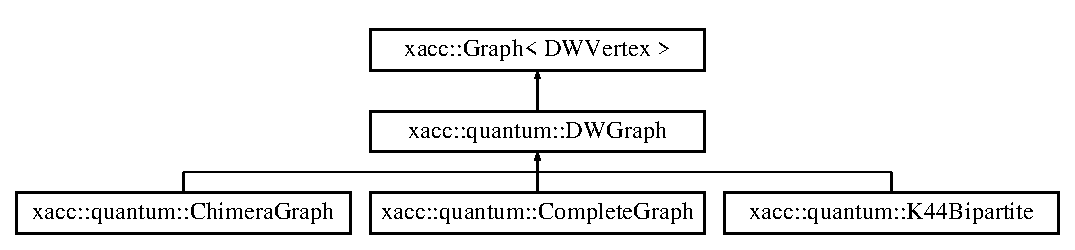
\includegraphics[height=2.916667cm]{a00030}
\end{center}
\end{figure}
\subsection*{Public Member Functions}
\begin{DoxyCompactItemize}
\item 
{\bfseries D\+W\+Graph} (const int n\+Vertices)\hypertarget{a00030_adc891c7ec39fbb480d9102c3b0458e4c}{}\label{a00030_adc891c7ec39fbb480d9102c3b0458e4c}

\item 
std\+::shared\+\_\+ptr$<$ \hyperlink{a00043}{Accelerator\+Graph} $>$ {\bfseries get\+Accelerator\+Graph} ()\hypertarget{a00030_acdce3a79dfc4e296c215ac95f6fef8f5}{}\label{a00030_acdce3a79dfc4e296c215ac95f6fef8f5}

\item 
std\+::string {\bfseries to\+Kernel\+Source} (const std\+::string \&kernel\+Name)\hypertarget{a00030_a636bf17193ae20ae6355755dacafdf98}{}\label{a00030_a636bf17193ae20ae6355755dacafdf98}

\end{DoxyCompactItemize}
\subsection*{Additional Inherited Members}


The documentation for this class was generated from the following file\+:\begin{DoxyCompactItemize}
\item 
D\+W\+Graph.\+hpp\end{DoxyCompactItemize}

\hypertarget{a00031}{}\section{xacc\+:\+:quantum\+:\+:D\+W\+IR Class Reference}
\label{a00031}\index{xacc\+::quantum\+::\+D\+W\+IR@{xacc\+::quantum\+::\+D\+W\+IR}}
Inheritance diagram for xacc\+:\+:quantum\+:\+:D\+W\+IR\+:\begin{figure}[H]
\begin{center}
\leavevmode
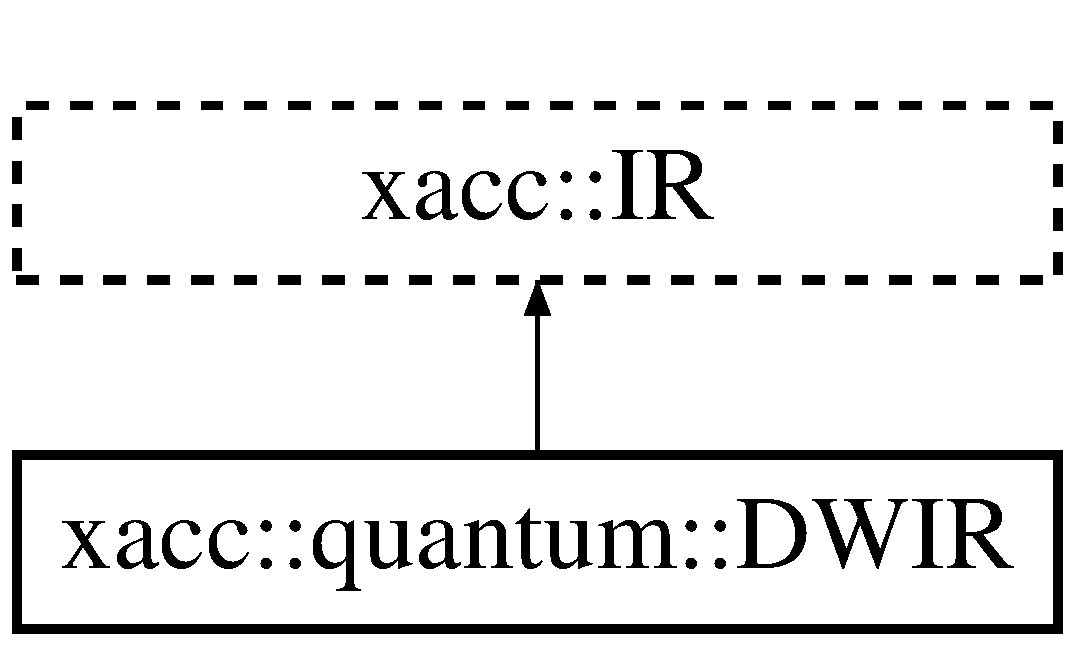
\includegraphics[height=2.000000cm]{a00031}
\end{center}
\end{figure}
\subsection*{Public Member Functions}
\begin{DoxyCompactItemize}
\item 
virtual std\+::string \hyperlink{a00031_a880cb60197577ea31115331e3a030e3e}{to\+Assembly\+String} (const std\+::string \&kernel\+Name, const std\+::string \&acc\+Buffer\+Var\+Name)
\item 
virtual void \hyperlink{a00031_abcbfd0a4cf697843391c65cbd9a82080}{persist} (std\+::ostream \&out\+Stream)
\item 
virtual void \hyperlink{a00031_a8b388d719d565bb902c979807d3d0d47}{load} (std\+::istream \&in\+Stream)
\item 
virtual void \hyperlink{a00031_af1bef18e1e9568d1313b03149aab8c1b}{add\+Kernel} (std\+::shared\+\_\+ptr$<$ \hyperlink{a00038}{Function} $>$ kernel)
\item 
virtual bool \hyperlink{a00031_ab5e8861d3bc0845bb015af6208f5f396}{kernel\+Exists} (const std\+::string \&name)
\item 
virtual std\+::shared\+\_\+ptr$<$ \hyperlink{a00038}{Function} $>$ \hyperlink{a00031_a38d8bdd24250749bc38ad31f8512fcfc}{get\+Kernel} (const std\+::string \&name)
\item 
virtual std\+::vector$<$ std\+::shared\+\_\+ptr$<$ \hyperlink{a00038}{Function} $>$ $>$ \hyperlink{a00031_a66e22c5dc95ec46045476864012ad08f}{get\+Kernels} ()
\end{DoxyCompactItemize}
\subsection*{Protected Attributes}
\begin{DoxyCompactItemize}
\item 
std\+::vector$<$ std\+::shared\+\_\+ptr$<$ \hyperlink{a00038}{Function} $>$ $>$ \hyperlink{a00031_abcb04ec3a152c3f22e5a757a9aecabf2}{kernels}
\end{DoxyCompactItemize}


\subsection{Member Function Documentation}
\index{xacc\+::quantum\+::\+D\+W\+IR@{xacc\+::quantum\+::\+D\+W\+IR}!add\+Kernel@{add\+Kernel}}
\index{add\+Kernel@{add\+Kernel}!xacc\+::quantum\+::\+D\+W\+IR@{xacc\+::quantum\+::\+D\+W\+IR}}
\subsubsection[{\texorpdfstring{add\+Kernel(std\+::shared\+\_\+ptr$<$ Function $>$ kernel)}{addKernel(std::shared\_ptr< Function > kernel)}}]{\setlength{\rightskip}{0pt plus 5cm}virtual void xacc\+::quantum\+::\+D\+W\+I\+R\+::add\+Kernel (
\begin{DoxyParamCaption}
\item[{std\+::shared\+\_\+ptr$<$ {\bf Function} $>$}]{kernel}
\end{DoxyParamCaption}
)\hspace{0.3cm}{\ttfamily [inline]}, {\ttfamily [virtual]}}\hypertarget{a00031_af1bef18e1e9568d1313b03149aab8c1b}{}\label{a00031_af1bef18e1e9568d1313b03149aab8c1b}
Add a new kernel to this \hyperlink{a00050}{IR} instance.


\begin{DoxyParams}{Parameters}
{\em kernel} & The \hyperlink{a00038}{Function} instance to add as a new kernel \\
\hline
\end{DoxyParams}


Implements \hyperlink{a00050_abbbf8e6993c518597de32cd05d49d737}{xacc\+::\+IR}.

\index{xacc\+::quantum\+::\+D\+W\+IR@{xacc\+::quantum\+::\+D\+W\+IR}!get\+Kernel@{get\+Kernel}}
\index{get\+Kernel@{get\+Kernel}!xacc\+::quantum\+::\+D\+W\+IR@{xacc\+::quantum\+::\+D\+W\+IR}}
\subsubsection[{\texorpdfstring{get\+Kernel(const std\+::string \&name)}{getKernel(const std::string \&name)}}]{\setlength{\rightskip}{0pt plus 5cm}virtual std\+::shared\+\_\+ptr$<${\bf Function}$>$ xacc\+::quantum\+::\+D\+W\+I\+R\+::get\+Kernel (
\begin{DoxyParamCaption}
\item[{const std\+::string \&}]{name}
\end{DoxyParamCaption}
)\hspace{0.3cm}{\ttfamily [inline]}, {\ttfamily [virtual]}}\hypertarget{a00031_a38d8bdd24250749bc38ad31f8512fcfc}{}\label{a00031_a38d8bdd24250749bc38ad31f8512fcfc}
Return the kernel with the given name.


\begin{DoxyParams}{Parameters}
{\em name} & The name of the kernel to return. \\
\hline
\end{DoxyParams}
\begin{DoxyReturn}{Returns}
kernel The kernel with given name. 
\end{DoxyReturn}


Implements \hyperlink{a00050_a6f49b4ba4b3a15142b04873284885f0d}{xacc\+::\+IR}.

\index{xacc\+::quantum\+::\+D\+W\+IR@{xacc\+::quantum\+::\+D\+W\+IR}!get\+Kernels@{get\+Kernels}}
\index{get\+Kernels@{get\+Kernels}!xacc\+::quantum\+::\+D\+W\+IR@{xacc\+::quantum\+::\+D\+W\+IR}}
\subsubsection[{\texorpdfstring{get\+Kernels()}{getKernels()}}]{\setlength{\rightskip}{0pt plus 5cm}virtual std\+::vector$<$std\+::shared\+\_\+ptr$<${\bf Function}$>$ $>$ xacc\+::quantum\+::\+D\+W\+I\+R\+::get\+Kernels (
\begin{DoxyParamCaption}
{}
\end{DoxyParamCaption}
)\hspace{0.3cm}{\ttfamily [inline]}, {\ttfamily [virtual]}}\hypertarget{a00031_a66e22c5dc95ec46045476864012ad08f}{}\label{a00031_a66e22c5dc95ec46045476864012ad08f}
Return all of this \hyperlink{a00050}{IR} instance\textquotesingle{}s kernels.

\begin{DoxyReturn}{Returns}
kernels The kernels this \hyperlink{a00050}{IR} contains. 
\end{DoxyReturn}


Implements \hyperlink{a00050_a88c50bfc5b279145360ddc0c3a703b9b}{xacc\+::\+IR}.

\index{xacc\+::quantum\+::\+D\+W\+IR@{xacc\+::quantum\+::\+D\+W\+IR}!kernel\+Exists@{kernel\+Exists}}
\index{kernel\+Exists@{kernel\+Exists}!xacc\+::quantum\+::\+D\+W\+IR@{xacc\+::quantum\+::\+D\+W\+IR}}
\subsubsection[{\texorpdfstring{kernel\+Exists(const std\+::string \&name)}{kernelExists(const std::string \&name)}}]{\setlength{\rightskip}{0pt plus 5cm}virtual bool xacc\+::quantum\+::\+D\+W\+I\+R\+::kernel\+Exists (
\begin{DoxyParamCaption}
\item[{const std\+::string \&}]{name}
\end{DoxyParamCaption}
)\hspace{0.3cm}{\ttfamily [inline]}, {\ttfamily [virtual]}}\hypertarget{a00031_ab5e8861d3bc0845bb015af6208f5f396}{}\label{a00031_ab5e8861d3bc0845bb015af6208f5f396}
Return true if the kernel with given name exists in this \hyperlink{a00050}{IR}.


\begin{DoxyParams}{Parameters}
{\em name} & The name of the kernel to return. \\
\hline
\end{DoxyParams}
\begin{DoxyReturn}{Returns}
exists True if kernel exists. 
\end{DoxyReturn}


Implements \hyperlink{a00050_afc9ccf5126f3fed19c2e879133b2f6d8}{xacc\+::\+IR}.

\index{xacc\+::quantum\+::\+D\+W\+IR@{xacc\+::quantum\+::\+D\+W\+IR}!load@{load}}
\index{load@{load}!xacc\+::quantum\+::\+D\+W\+IR@{xacc\+::quantum\+::\+D\+W\+IR}}
\subsubsection[{\texorpdfstring{load(std\+::istream \&in\+Stream)}{load(std::istream \&inStream)}}]{\setlength{\rightskip}{0pt plus 5cm}virtual void xacc\+::quantum\+::\+D\+W\+I\+R\+::load (
\begin{DoxyParamCaption}
\item[{std\+::istream \&}]{in\+Stream}
\end{DoxyParamCaption}
)\hspace{0.3cm}{\ttfamily [inline]}, {\ttfamily [virtual]}}\hypertarget{a00031_a8b388d719d565bb902c979807d3d0d47}{}\label{a00031_a8b388d719d565bb902c979807d3d0d47}
Create this \hyperlink{a00050}{IR} instance from the given input stream.


\begin{DoxyParams}{Parameters}
{\em in\+Stream} & \\
\hline
\end{DoxyParams}


Implements \hyperlink{a00050_a444c2e4dc0faac500fb70fa93997e9bc}{xacc\+::\+IR}.

\index{xacc\+::quantum\+::\+D\+W\+IR@{xacc\+::quantum\+::\+D\+W\+IR}!persist@{persist}}
\index{persist@{persist}!xacc\+::quantum\+::\+D\+W\+IR@{xacc\+::quantum\+::\+D\+W\+IR}}
\subsubsection[{\texorpdfstring{persist(std\+::ostream \&out\+Stream)}{persist(std::ostream \&outStream)}}]{\setlength{\rightskip}{0pt plus 5cm}virtual void xacc\+::quantum\+::\+D\+W\+I\+R\+::persist (
\begin{DoxyParamCaption}
\item[{std\+::ostream \&}]{out\+Stream}
\end{DoxyParamCaption}
)\hspace{0.3cm}{\ttfamily [inline]}, {\ttfamily [virtual]}}\hypertarget{a00031_abcbfd0a4cf697843391c65cbd9a82080}{}\label{a00031_abcbfd0a4cf697843391c65cbd9a82080}
Persist this \hyperlink{a00050}{IR} instance to the given output stream.


\begin{DoxyParams}{Parameters}
{\em out\+Stream} & \\
\hline
\end{DoxyParams}


Implements \hyperlink{a00050_a414b72224d88473ad6190bb88102a3ea}{xacc\+::\+IR}.

\index{xacc\+::quantum\+::\+D\+W\+IR@{xacc\+::quantum\+::\+D\+W\+IR}!to\+Assembly\+String@{to\+Assembly\+String}}
\index{to\+Assembly\+String@{to\+Assembly\+String}!xacc\+::quantum\+::\+D\+W\+IR@{xacc\+::quantum\+::\+D\+W\+IR}}
\subsubsection[{\texorpdfstring{to\+Assembly\+String(const std\+::string \&kernel\+Name, const std\+::string \&acc\+Buffer\+Var\+Name)}{toAssemblyString(const std::string \&kernelName, const std::string \&accBufferVarName)}}]{\setlength{\rightskip}{0pt plus 5cm}virtual std\+::string xacc\+::quantum\+::\+D\+W\+I\+R\+::to\+Assembly\+String (
\begin{DoxyParamCaption}
\item[{const std\+::string \&}]{kernel\+Name, }
\item[{const std\+::string \&}]{acc\+Buffer\+Var\+Name}
\end{DoxyParamCaption}
)\hspace{0.3cm}{\ttfamily [inline]}, {\ttfamily [virtual]}}\hypertarget{a00031_a880cb60197577ea31115331e3a030e3e}{}\label{a00031_a880cb60197577ea31115331e3a030e3e}
Return a assembly-\/like string representation of this intermediate representation \begin{DoxyReturn}{Returns}

\end{DoxyReturn}


Implements \hyperlink{a00050_a8356cdff1919b88eabeb84fd7450cdb6}{xacc\+::\+IR}.



\subsection{Member Data Documentation}
\index{xacc\+::quantum\+::\+D\+W\+IR@{xacc\+::quantum\+::\+D\+W\+IR}!kernels@{kernels}}
\index{kernels@{kernels}!xacc\+::quantum\+::\+D\+W\+IR@{xacc\+::quantum\+::\+D\+W\+IR}}
\subsubsection[{\texorpdfstring{kernels}{kernels}}]{\setlength{\rightskip}{0pt plus 5cm}std\+::vector$<$std\+::shared\+\_\+ptr$<${\bf Function}$>$ $>$ xacc\+::quantum\+::\+D\+W\+I\+R\+::kernels\hspace{0.3cm}{\ttfamily [protected]}}\hypertarget{a00031_abcb04ec3a152c3f22e5a757a9aecabf2}{}\label{a00031_abcb04ec3a152c3f22e5a757a9aecabf2}
Reference to this Q\+IR\textquotesingle{}s list of quantum functions 

The documentation for this class was generated from the following file\+:\begin{DoxyCompactItemize}
\item 
D\+W\+I\+R.\+hpp\end{DoxyCompactItemize}

\hypertarget{a00032}{}\section{xacc\+:\+:quantum\+:\+:D\+W\+Kernel Class Reference}
\label{a00032}\index{xacc\+::quantum\+::\+D\+W\+Kernel@{xacc\+::quantum\+::\+D\+W\+Kernel}}


{\ttfamily \#include $<$D\+W\+Kernel.\+hpp$>$}

Inheritance diagram for xacc\+:\+:quantum\+:\+:D\+W\+Kernel\+:\begin{figure}[H]
\begin{center}
\leavevmode
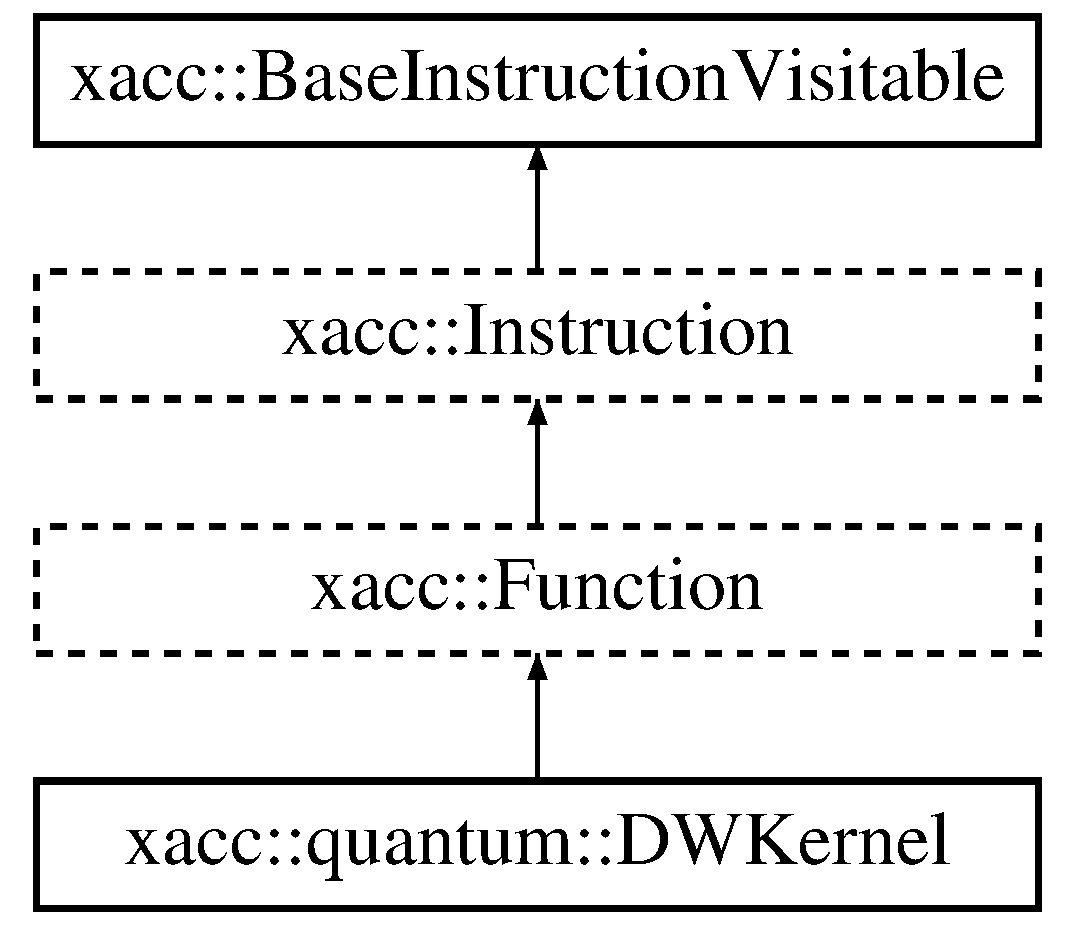
\includegraphics[height=4.000000cm]{a00032}
\end{center}
\end{figure}
\subsection*{Public Member Functions}
\begin{DoxyCompactItemize}
\item 
\hyperlink{a00032_a76a4dfadb973abbc93d1afefc6839ad8}{D\+W\+Kernel} (std\+::string kernel\+Name)
\item 
virtual const int \hyperlink{a00032_a79aecc7419a20b8779372ef36fc24806}{n\+Instructions} ()
\item 
virtual Inst\+Ptr \hyperlink{a00032_a00f23cd2e15ea6b9d00d4f3dbe1540f8}{get\+Instruction} (const int idx)
\item 
virtual std\+::list$<$ Inst\+Ptr $>$ \hyperlink{a00032_abbb8f2b1c78623c377524e45d581d018}{get\+Instructions} ()
\item 
virtual void \hyperlink{a00032_af2bcfd679e6cb89194f3f0bff8622b99}{remove\+Instruction} (const int idx)
\item 
virtual void \hyperlink{a00032_a4c3043d6971999c3a09e797fc55deb6c}{add\+Instruction} (Inst\+Ptr instruction)
\item 
virtual void \hyperlink{a00032_a75eb3560d2f81c9a5ae1cf765deb0e83}{replace\+Instruction} (const int idx, Inst\+Ptr replacing\+Inst)
\item 
virtual void \hyperlink{a00032_a1627af0141f70fc4a3cd500a13fb31b8}{insert\+Instruction} (const int idx, Inst\+Ptr new\+Inst)
\item 
virtual const std\+::string \hyperlink{a00032_a7f0c4d3c73029566561cf56a474bcbbd}{get\+Name} ()
\item 
virtual const std\+::vector$<$ int $>$ \hyperlink{a00032_adae68964db6acd8b4c2267c270a8ec58}{bits} ()
\item 
virtual const std\+::string \hyperlink{a00032_adbc3fdd080ebba20bc620b8832979f16}{to\+String} (const std\+::string \&buffer\+Var\+Name)
\item 
std\+::vector$<$ double $>$ {\bfseries get\+All\+Biases} ()\hypertarget{a00032_a9ee05b3d7689bbf837bdb7737f9745f4}{}\label{a00032_a9ee05b3d7689bbf837bdb7737f9745f4}

\item 
std\+::vector$<$ double $>$ {\bfseries get\+All\+Couplers} ()\hypertarget{a00032_a7df03ecec9c1821433daa3aa092cbd4d}{}\label{a00032_a7df03ecec9c1821433daa3aa092cbd4d}

\item 
virtual Instruction\+Parameter \hyperlink{a00032_a81711b7db284aba35d6952e4d1d15d41}{get\+Parameter} (const int idx)
\item 
virtual void \hyperlink{a00032_adf89cdd1f54e183c4cff36b338b2be8d}{set\+Parameter} (const int idx, Instruction\+Parameter \&p)
\item 
virtual std\+::vector$<$ Instruction\+Parameter $>$ \hyperlink{a00032_a829462cff34e2257da06afd8a2051a8e}{get\+Parameters} ()
\item 
virtual bool \hyperlink{a00032_a8957ea368244ed4a4ebd85f6bfecb785}{is\+Parameterized} ()
\item 
virtual const int \hyperlink{a00032_a029429948329b94c1d89f32cf5c486d4}{n\+Parameters} ()
\item 
virtual void \hyperlink{a00032_a09ffac417d4ecbbd82d7a680ad8dfcce}{evaluate\+Variable\+Parameters} (std\+::vector$<$ Instruction\+Parameter $>$ parameters)
\end{DoxyCompactItemize}
\subsection*{Protected Attributes}
\begin{DoxyCompactItemize}
\item 
std\+::list$<$ Inst\+Ptr $>$ {\bfseries instructions}\hypertarget{a00032_a38e434be6ef46a1ff43744632ae59ea8}{}\label{a00032_a38e434be6ef46a1ff43744632ae59ea8}

\item 
std\+::string {\bfseries name}\hypertarget{a00032_a0df03f85cc3b8a4cd1a7fc839d4d303c}{}\label{a00032_a0df03f85cc3b8a4cd1a7fc839d4d303c}

\end{DoxyCompactItemize}
\subsection*{Additional Inherited Members}


\subsection{Detailed Description}
The \hyperlink{a00032}{D\+W\+Kernel} is an X\+A\+CC \hyperlink{a00038}{Function} that contains \hyperlink{a00033}{D\+W\+Q\+MI} Instructions. 

\subsection{Constructor \& Destructor Documentation}
\index{xacc\+::quantum\+::\+D\+W\+Kernel@{xacc\+::quantum\+::\+D\+W\+Kernel}!D\+W\+Kernel@{D\+W\+Kernel}}
\index{D\+W\+Kernel@{D\+W\+Kernel}!xacc\+::quantum\+::\+D\+W\+Kernel@{xacc\+::quantum\+::\+D\+W\+Kernel}}
\subsubsection[{\texorpdfstring{D\+W\+Kernel(std\+::string kernel\+Name)}{DWKernel(std::string kernelName)}}]{\setlength{\rightskip}{0pt plus 5cm}xacc\+::quantum\+::\+D\+W\+Kernel\+::\+D\+W\+Kernel (
\begin{DoxyParamCaption}
\item[{std\+::string}]{kernel\+Name}
\end{DoxyParamCaption}
)\hspace{0.3cm}{\ttfamily [inline]}}\hypertarget{a00032_a76a4dfadb973abbc93d1afefc6839ad8}{}\label{a00032_a76a4dfadb973abbc93d1afefc6839ad8}
The constructor, takes the function unique id and its name.


\begin{DoxyParams}{Parameters}
{\em id} & \\
\hline
{\em name} & \\
\hline
\end{DoxyParams}


\subsection{Member Function Documentation}
\index{xacc\+::quantum\+::\+D\+W\+Kernel@{xacc\+::quantum\+::\+D\+W\+Kernel}!add\+Instruction@{add\+Instruction}}
\index{add\+Instruction@{add\+Instruction}!xacc\+::quantum\+::\+D\+W\+Kernel@{xacc\+::quantum\+::\+D\+W\+Kernel}}
\subsubsection[{\texorpdfstring{add\+Instruction(\+Inst\+Ptr instruction)}{addInstruction(InstPtr instruction)}}]{\setlength{\rightskip}{0pt plus 5cm}virtual void xacc\+::quantum\+::\+D\+W\+Kernel\+::add\+Instruction (
\begin{DoxyParamCaption}
\item[{Inst\+Ptr}]{instruction}
\end{DoxyParamCaption}
)\hspace{0.3cm}{\ttfamily [inline]}, {\ttfamily [virtual]}}\hypertarget{a00032_a4c3043d6971999c3a09e797fc55deb6c}{}\label{a00032_a4c3043d6971999c3a09e797fc55deb6c}
Add an instruction to this quantum intermediate representation.


\begin{DoxyParams}{Parameters}
{\em instruction} & \\
\hline
\end{DoxyParams}


Implements \hyperlink{a00038_aa8c9ec2d08be75c69399d4254b0216f5}{xacc\+::\+Function}.

\index{xacc\+::quantum\+::\+D\+W\+Kernel@{xacc\+::quantum\+::\+D\+W\+Kernel}!bits@{bits}}
\index{bits@{bits}!xacc\+::quantum\+::\+D\+W\+Kernel@{xacc\+::quantum\+::\+D\+W\+Kernel}}
\subsubsection[{\texorpdfstring{bits()}{bits()}}]{\setlength{\rightskip}{0pt plus 5cm}virtual const std\+::vector$<$int$>$ xacc\+::quantum\+::\+D\+W\+Kernel\+::bits (
\begin{DoxyParamCaption}
{}
\end{DoxyParamCaption}
)\hspace{0.3cm}{\ttfamily [inline]}, {\ttfamily [virtual]}}\hypertarget{a00032_adae68964db6acd8b4c2267c270a8ec58}{}\label{a00032_adae68964db6acd8b4c2267c270a8ec58}
Return the qubits this function acts on. \begin{DoxyReturn}{Returns}

\end{DoxyReturn}


Implements \hyperlink{a00046_a819f32e94c3e1c9e69a0061aaf8d86dc}{xacc\+::\+Instruction}.

\index{xacc\+::quantum\+::\+D\+W\+Kernel@{xacc\+::quantum\+::\+D\+W\+Kernel}!evaluate\+Variable\+Parameters@{evaluate\+Variable\+Parameters}}
\index{evaluate\+Variable\+Parameters@{evaluate\+Variable\+Parameters}!xacc\+::quantum\+::\+D\+W\+Kernel@{xacc\+::quantum\+::\+D\+W\+Kernel}}
\subsubsection[{\texorpdfstring{evaluate\+Variable\+Parameters(std\+::vector$<$ Instruction\+Parameter $>$ parameters)}{evaluateVariableParameters(std::vector< InstructionParameter > parameters)}}]{\setlength{\rightskip}{0pt plus 5cm}virtual void xacc\+::quantum\+::\+D\+W\+Kernel\+::evaluate\+Variable\+Parameters (
\begin{DoxyParamCaption}
\item[{std\+::vector$<$ Instruction\+Parameter $>$}]{parameters}
\end{DoxyParamCaption}
)\hspace{0.3cm}{\ttfamily [inline]}, {\ttfamily [virtual]}}\hypertarget{a00032_a09ffac417d4ecbbd82d7a680ad8dfcce}{}\label{a00032_a09ffac417d4ecbbd82d7a680ad8dfcce}
This method is used to evaluate this \hyperlink{a00038}{Function}\textquotesingle{}s parameterized Instructions that have string variable Instruction\+Parameters. These parameters are updated with the given runtime parameters.


\begin{DoxyParams}{Parameters}
{\em parameters} & The runtime parameters \\
\hline
\end{DoxyParams}


Implements \hyperlink{a00038_af6ae9453027789a2aaec30e59c9e45e3}{xacc\+::\+Function}.

\index{xacc\+::quantum\+::\+D\+W\+Kernel@{xacc\+::quantum\+::\+D\+W\+Kernel}!get\+Instruction@{get\+Instruction}}
\index{get\+Instruction@{get\+Instruction}!xacc\+::quantum\+::\+D\+W\+Kernel@{xacc\+::quantum\+::\+D\+W\+Kernel}}
\subsubsection[{\texorpdfstring{get\+Instruction(const int idx)}{getInstruction(const int idx)}}]{\setlength{\rightskip}{0pt plus 5cm}virtual Inst\+Ptr xacc\+::quantum\+::\+D\+W\+Kernel\+::get\+Instruction (
\begin{DoxyParamCaption}
\item[{const int}]{idx}
\end{DoxyParamCaption}
)\hspace{0.3cm}{\ttfamily [inline]}, {\ttfamily [virtual]}}\hypertarget{a00032_a00f23cd2e15ea6b9d00d4f3dbe1540f8}{}\label{a00032_a00f23cd2e15ea6b9d00d4f3dbe1540f8}
Return the \hyperlink{a00046}{Instruction} at the given index.


\begin{DoxyParams}{Parameters}
{\em idx} & The desired \hyperlink{a00046}{Instruction} index \\
\hline
\end{DoxyParams}
\begin{DoxyReturn}{Returns}
inst The instruction at the given index. 
\end{DoxyReturn}


Implements \hyperlink{a00038_afa549fc91b5a05f26d8139954a7e0ed5}{xacc\+::\+Function}.

\index{xacc\+::quantum\+::\+D\+W\+Kernel@{xacc\+::quantum\+::\+D\+W\+Kernel}!get\+Instructions@{get\+Instructions}}
\index{get\+Instructions@{get\+Instructions}!xacc\+::quantum\+::\+D\+W\+Kernel@{xacc\+::quantum\+::\+D\+W\+Kernel}}
\subsubsection[{\texorpdfstring{get\+Instructions()}{getInstructions()}}]{\setlength{\rightskip}{0pt plus 5cm}virtual std\+::list$<$Inst\+Ptr$>$ xacc\+::quantum\+::\+D\+W\+Kernel\+::get\+Instructions (
\begin{DoxyParamCaption}
{}
\end{DoxyParamCaption}
)\hspace{0.3cm}{\ttfamily [inline]}, {\ttfamily [virtual]}}\hypertarget{a00032_abbb8f2b1c78623c377524e45d581d018}{}\label{a00032_abbb8f2b1c78623c377524e45d581d018}
Return all Instructions in this \hyperlink{a00038}{Function}

\begin{DoxyReturn}{Returns}
insts The list of this \hyperlink{a00038}{Function}\textquotesingle{}s Instructions 
\end{DoxyReturn}


Implements \hyperlink{a00038_aaf80bd3d49113a92b520785572663032}{xacc\+::\+Function}.

\index{xacc\+::quantum\+::\+D\+W\+Kernel@{xacc\+::quantum\+::\+D\+W\+Kernel}!get\+Name@{get\+Name}}
\index{get\+Name@{get\+Name}!xacc\+::quantum\+::\+D\+W\+Kernel@{xacc\+::quantum\+::\+D\+W\+Kernel}}
\subsubsection[{\texorpdfstring{get\+Name()}{getName()}}]{\setlength{\rightskip}{0pt plus 5cm}virtual const std\+::string xacc\+::quantum\+::\+D\+W\+Kernel\+::get\+Name (
\begin{DoxyParamCaption}
{}
\end{DoxyParamCaption}
)\hspace{0.3cm}{\ttfamily [inline]}, {\ttfamily [virtual]}}\hypertarget{a00032_a7f0c4d3c73029566561cf56a474bcbbd}{}\label{a00032_a7f0c4d3c73029566561cf56a474bcbbd}
Return the name of this function \begin{DoxyReturn}{Returns}

\end{DoxyReturn}


Implements \hyperlink{a00046_ac7ff23f693e2276edbf3fdac5452792c}{xacc\+::\+Instruction}.

\index{xacc\+::quantum\+::\+D\+W\+Kernel@{xacc\+::quantum\+::\+D\+W\+Kernel}!get\+Parameter@{get\+Parameter}}
\index{get\+Parameter@{get\+Parameter}!xacc\+::quantum\+::\+D\+W\+Kernel@{xacc\+::quantum\+::\+D\+W\+Kernel}}
\subsubsection[{\texorpdfstring{get\+Parameter(const int idx)}{getParameter(const int idx)}}]{\setlength{\rightskip}{0pt plus 5cm}virtual Instruction\+Parameter xacc\+::quantum\+::\+D\+W\+Kernel\+::get\+Parameter (
\begin{DoxyParamCaption}
\item[{const int}]{idx}
\end{DoxyParamCaption}
)\hspace{0.3cm}{\ttfamily [inline]}, {\ttfamily [virtual]}}\hypertarget{a00032_a81711b7db284aba35d6952e4d1d15d41}{}\label{a00032_a81711b7db284aba35d6952e4d1d15d41}
Return this \hyperlink{a00046}{Instruction}\textquotesingle{}s parameter at the given index.


\begin{DoxyParams}{Parameters}
{\em idx} & The index of the parameter. \\
\hline
\end{DoxyParams}
\begin{DoxyReturn}{Returns}
param The Instruction\+Parameter at the given index. 
\end{DoxyReturn}


Implements \hyperlink{a00046_aa0d9de97a4833a042379647f83c33ab6}{xacc\+::\+Instruction}.

\index{xacc\+::quantum\+::\+D\+W\+Kernel@{xacc\+::quantum\+::\+D\+W\+Kernel}!get\+Parameters@{get\+Parameters}}
\index{get\+Parameters@{get\+Parameters}!xacc\+::quantum\+::\+D\+W\+Kernel@{xacc\+::quantum\+::\+D\+W\+Kernel}}
\subsubsection[{\texorpdfstring{get\+Parameters()}{getParameters()}}]{\setlength{\rightskip}{0pt plus 5cm}virtual std\+::vector$<$Instruction\+Parameter$>$ xacc\+::quantum\+::\+D\+W\+Kernel\+::get\+Parameters (
\begin{DoxyParamCaption}
{}
\end{DoxyParamCaption}
)\hspace{0.3cm}{\ttfamily [inline]}, {\ttfamily [virtual]}}\hypertarget{a00032_a829462cff34e2257da06afd8a2051a8e}{}\label{a00032_a829462cff34e2257da06afd8a2051a8e}
Return all of this \hyperlink{a00046}{Instruction}\textquotesingle{}s parameters.

\begin{DoxyReturn}{Returns}
params This instructions parameters. 
\end{DoxyReturn}


Implements \hyperlink{a00046_aeb67c67713896e8f27a5c7dd531f3340}{xacc\+::\+Instruction}.

\index{xacc\+::quantum\+::\+D\+W\+Kernel@{xacc\+::quantum\+::\+D\+W\+Kernel}!insert\+Instruction@{insert\+Instruction}}
\index{insert\+Instruction@{insert\+Instruction}!xacc\+::quantum\+::\+D\+W\+Kernel@{xacc\+::quantum\+::\+D\+W\+Kernel}}
\subsubsection[{\texorpdfstring{insert\+Instruction(const int idx, Inst\+Ptr new\+Inst)}{insertInstruction(const int idx, InstPtr newInst)}}]{\setlength{\rightskip}{0pt plus 5cm}virtual void xacc\+::quantum\+::\+D\+W\+Kernel\+::insert\+Instruction (
\begin{DoxyParamCaption}
\item[{const int}]{idx, }
\item[{Inst\+Ptr}]{new\+Inst}
\end{DoxyParamCaption}
)\hspace{0.3cm}{\ttfamily [inline]}, {\ttfamily [virtual]}}\hypertarget{a00032_a1627af0141f70fc4a3cd500a13fb31b8}{}\label{a00032_a1627af0141f70fc4a3cd500a13fb31b8}
Insert a new \hyperlink{a00046}{Instruction} at the given index. All previous instructions are pushed back, ie their new indices are current\+Index + 1.


\begin{DoxyParams}{Parameters}
{\em idx} & The index where the new instruction should be inserted \\
\hline
{\em new\+Inst} & The new \hyperlink{a00046}{Instruction} to insert. \\
\hline
\end{DoxyParams}


Implements \hyperlink{a00038_acde702e44bdbc2759b338365218d7ebe}{xacc\+::\+Function}.

\index{xacc\+::quantum\+::\+D\+W\+Kernel@{xacc\+::quantum\+::\+D\+W\+Kernel}!is\+Parameterized@{is\+Parameterized}}
\index{is\+Parameterized@{is\+Parameterized}!xacc\+::quantum\+::\+D\+W\+Kernel@{xacc\+::quantum\+::\+D\+W\+Kernel}}
\subsubsection[{\texorpdfstring{is\+Parameterized()}{isParameterized()}}]{\setlength{\rightskip}{0pt plus 5cm}virtual bool xacc\+::quantum\+::\+D\+W\+Kernel\+::is\+Parameterized (
\begin{DoxyParamCaption}
{}
\end{DoxyParamCaption}
)\hspace{0.3cm}{\ttfamily [inline]}, {\ttfamily [virtual]}}\hypertarget{a00032_a8957ea368244ed4a4ebd85f6bfecb785}{}\label{a00032_a8957ea368244ed4a4ebd85f6bfecb785}
Return true if this \hyperlink{a00046}{Instruction} is parameterized.

\begin{DoxyReturn}{Returns}
parameterized True if this \hyperlink{a00046}{Instruction} has parameters. 
\end{DoxyReturn}


Reimplemented from \hyperlink{a00046_a7b24d8ae485369fc2b2df7a3224a5e26}{xacc\+::\+Instruction}.

\index{xacc\+::quantum\+::\+D\+W\+Kernel@{xacc\+::quantum\+::\+D\+W\+Kernel}!n\+Instructions@{n\+Instructions}}
\index{n\+Instructions@{n\+Instructions}!xacc\+::quantum\+::\+D\+W\+Kernel@{xacc\+::quantum\+::\+D\+W\+Kernel}}
\subsubsection[{\texorpdfstring{n\+Instructions()}{nInstructions()}}]{\setlength{\rightskip}{0pt plus 5cm}virtual const int xacc\+::quantum\+::\+D\+W\+Kernel\+::n\+Instructions (
\begin{DoxyParamCaption}
{}
\end{DoxyParamCaption}
)\hspace{0.3cm}{\ttfamily [inline]}, {\ttfamily [virtual]}}\hypertarget{a00032_a79aecc7419a20b8779372ef36fc24806}{}\label{a00032_a79aecc7419a20b8779372ef36fc24806}
Return the number of Instructions that this \hyperlink{a00038}{Function} contains.

\begin{DoxyReturn}{Returns}
n\+Inst The number of instructions 
\end{DoxyReturn}


Implements \hyperlink{a00038_a8901985525f59713e14c61713e07c086}{xacc\+::\+Function}.

\index{xacc\+::quantum\+::\+D\+W\+Kernel@{xacc\+::quantum\+::\+D\+W\+Kernel}!n\+Parameters@{n\+Parameters}}
\index{n\+Parameters@{n\+Parameters}!xacc\+::quantum\+::\+D\+W\+Kernel@{xacc\+::quantum\+::\+D\+W\+Kernel}}
\subsubsection[{\texorpdfstring{n\+Parameters()}{nParameters()}}]{\setlength{\rightskip}{0pt plus 5cm}virtual const int xacc\+::quantum\+::\+D\+W\+Kernel\+::n\+Parameters (
\begin{DoxyParamCaption}
{}
\end{DoxyParamCaption}
)\hspace{0.3cm}{\ttfamily [inline]}, {\ttfamily [virtual]}}\hypertarget{a00032_a029429948329b94c1d89f32cf5c486d4}{}\label{a00032_a029429948329b94c1d89f32cf5c486d4}
Return the number of Instruction\+Parameters this \hyperlink{a00046}{Instruction} contains.

\begin{DoxyReturn}{Returns}
n\+Insts The number of instructions. 
\end{DoxyReturn}


Implements \hyperlink{a00046_ad54585d13c04ffd20296fff7ab8107ff}{xacc\+::\+Instruction}.

\index{xacc\+::quantum\+::\+D\+W\+Kernel@{xacc\+::quantum\+::\+D\+W\+Kernel}!remove\+Instruction@{remove\+Instruction}}
\index{remove\+Instruction@{remove\+Instruction}!xacc\+::quantum\+::\+D\+W\+Kernel@{xacc\+::quantum\+::\+D\+W\+Kernel}}
\subsubsection[{\texorpdfstring{remove\+Instruction(const int idx)}{removeInstruction(const int idx)}}]{\setlength{\rightskip}{0pt plus 5cm}virtual void xacc\+::quantum\+::\+D\+W\+Kernel\+::remove\+Instruction (
\begin{DoxyParamCaption}
\item[{const int}]{idx}
\end{DoxyParamCaption}
)\hspace{0.3cm}{\ttfamily [inline]}, {\ttfamily [virtual]}}\hypertarget{a00032_af2bcfd679e6cb89194f3f0bff8622b99}{}\label{a00032_af2bcfd679e6cb89194f3f0bff8622b99}
Remove the \hyperlink{a00046}{Instruction} at the given index.


\begin{DoxyParams}{Parameters}
{\em idx} & The index of the \hyperlink{a00046}{Instruction} to remove. \\
\hline
\end{DoxyParams}


Implements \hyperlink{a00038_ab6478b09bb28e194bb555b3180737733}{xacc\+::\+Function}.

\index{xacc\+::quantum\+::\+D\+W\+Kernel@{xacc\+::quantum\+::\+D\+W\+Kernel}!replace\+Instruction@{replace\+Instruction}}
\index{replace\+Instruction@{replace\+Instruction}!xacc\+::quantum\+::\+D\+W\+Kernel@{xacc\+::quantum\+::\+D\+W\+Kernel}}
\subsubsection[{\texorpdfstring{replace\+Instruction(const int idx, Inst\+Ptr replacing\+Inst)}{replaceInstruction(const int idx, InstPtr replacingInst)}}]{\setlength{\rightskip}{0pt plus 5cm}virtual void xacc\+::quantum\+::\+D\+W\+Kernel\+::replace\+Instruction (
\begin{DoxyParamCaption}
\item[{const int}]{idx, }
\item[{Inst\+Ptr}]{replacing\+Inst}
\end{DoxyParamCaption}
)\hspace{0.3cm}{\ttfamily [inline]}, {\ttfamily [virtual]}}\hypertarget{a00032_a75eb3560d2f81c9a5ae1cf765deb0e83}{}\label{a00032_a75eb3560d2f81c9a5ae1cf765deb0e83}
Replace the given current quantum instruction with the new replacing\+Inst quantum \hyperlink{a00046}{Instruction}.


\begin{DoxyParams}{Parameters}
{\em current\+Inst} & \\
\hline
{\em replacing\+Inst} & \\
\hline
\end{DoxyParams}


Implements \hyperlink{a00038_a2ef6a4923a6734f90f6ee3d94d263af0}{xacc\+::\+Function}.

\index{xacc\+::quantum\+::\+D\+W\+Kernel@{xacc\+::quantum\+::\+D\+W\+Kernel}!set\+Parameter@{set\+Parameter}}
\index{set\+Parameter@{set\+Parameter}!xacc\+::quantum\+::\+D\+W\+Kernel@{xacc\+::quantum\+::\+D\+W\+Kernel}}
\subsubsection[{\texorpdfstring{set\+Parameter(const int idx, Instruction\+Parameter \&p)}{setParameter(const int idx, InstructionParameter \&p)}}]{\setlength{\rightskip}{0pt plus 5cm}virtual void xacc\+::quantum\+::\+D\+W\+Kernel\+::set\+Parameter (
\begin{DoxyParamCaption}
\item[{const int}]{idx, }
\item[{Instruction\+Parameter \&}]{isnt}
\end{DoxyParamCaption}
)\hspace{0.3cm}{\ttfamily [inline]}, {\ttfamily [virtual]}}\hypertarget{a00032_adf89cdd1f54e183c4cff36b338b2be8d}{}\label{a00032_adf89cdd1f54e183c4cff36b338b2be8d}
Set this \hyperlink{a00046}{Instruction}\textquotesingle{}s parameter at the given index.


\begin{DoxyParams}{Parameters}
{\em idx} & The index of the parameter \\
\hline
{\em inst} & The instruction. \\
\hline
\end{DoxyParams}


Implements \hyperlink{a00046_a407a0ac662fa0b1ec3e301e8ff9bade7}{xacc\+::\+Instruction}.

\index{xacc\+::quantum\+::\+D\+W\+Kernel@{xacc\+::quantum\+::\+D\+W\+Kernel}!to\+String@{to\+String}}
\index{to\+String@{to\+String}!xacc\+::quantum\+::\+D\+W\+Kernel@{xacc\+::quantum\+::\+D\+W\+Kernel}}
\subsubsection[{\texorpdfstring{to\+String(const std\+::string \&buffer\+Var\+Name)}{toString(const std::string \&bufferVarName)}}]{\setlength{\rightskip}{0pt plus 5cm}virtual const std\+::string xacc\+::quantum\+::\+D\+W\+Kernel\+::to\+String (
\begin{DoxyParamCaption}
\item[{const std\+::string \&}]{buffer\+Var\+Name}
\end{DoxyParamCaption}
)\hspace{0.3cm}{\ttfamily [inline]}, {\ttfamily [virtual]}}\hypertarget{a00032_adbc3fdd080ebba20bc620b8832979f16}{}\label{a00032_adbc3fdd080ebba20bc620b8832979f16}
Return an assembly-\/like string representation for this function . 
\begin{DoxyParams}{Parameters}
{\em buffer\+Var\+Name} & \\
\hline
\end{DoxyParams}
\begin{DoxyReturn}{Returns}

\end{DoxyReturn}


Implements \hyperlink{a00046_ae94c2d089908294c1d410b14c96817ae}{xacc\+::\+Instruction}.



The documentation for this class was generated from the following file\+:\begin{DoxyCompactItemize}
\item 
D\+W\+Kernel.\+hpp\end{DoxyCompactItemize}

\hypertarget{a00033}{}\section{xacc\+:\+:quantum\+:\+:D\+W\+Q\+MI Class Reference}
\label{a00033}\index{xacc\+::quantum\+::\+D\+W\+Q\+MI@{xacc\+::quantum\+::\+D\+W\+Q\+MI}}


{\ttfamily \#include $<$D\+W\+Q\+M\+I.\+hpp$>$}

Inheritance diagram for xacc\+:\+:quantum\+:\+:D\+W\+Q\+MI\+:\begin{figure}[H]
\begin{center}
\leavevmode
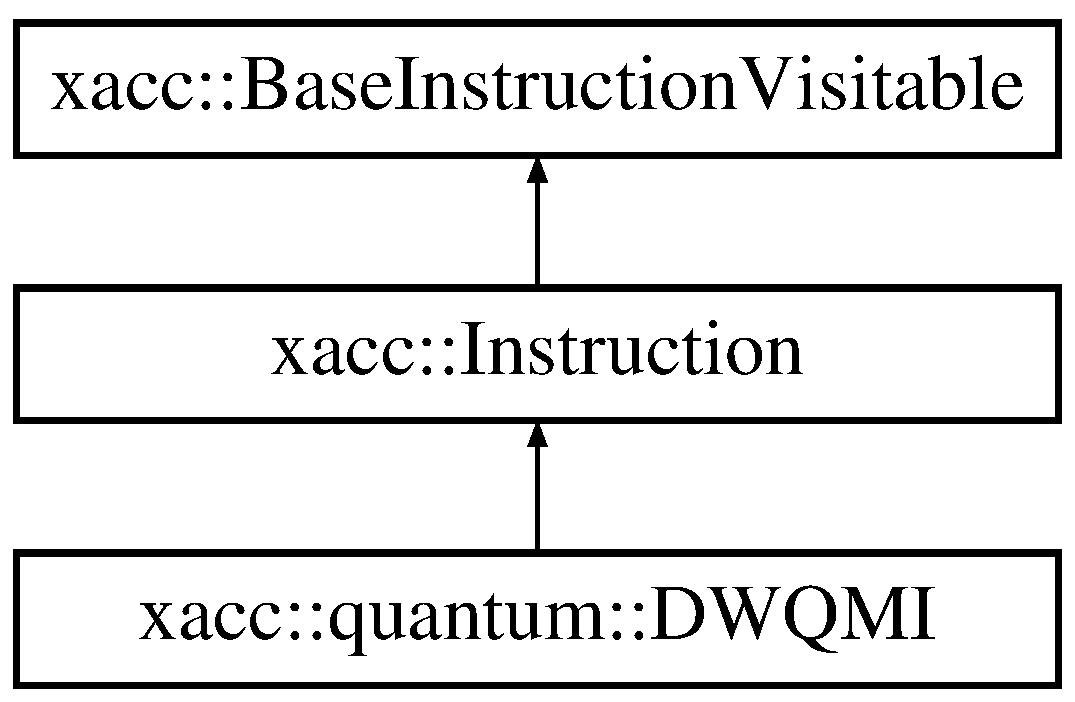
\includegraphics[height=3.000000cm]{a00033}
\end{center}
\end{figure}
\subsection*{Public Member Functions}
\begin{DoxyCompactItemize}
\item 
\hyperlink{a00033_a7fa74443cf18934c1f166e8343eada48}{D\+W\+Q\+MI} (int qbit)
\item 
\hyperlink{a00033_a219507677fcdf59ee0ddfa8c78e59539}{D\+W\+Q\+MI} (int qbit, double param)
\item 
\hyperlink{a00033_aabe1dbbc737114b2f96434592e1f115a}{D\+W\+Q\+MI} (int qbit1, int qbit2, double param)
\item 
virtual const std\+::string \hyperlink{a00033_ad93428eb61adade7bb99c7633bb02aca}{get\+Name} ()
\item 
virtual const std\+::string \hyperlink{a00033_a8d8742bb6743cf6e49f95966d05bbec2}{to\+String} (const std\+::string \&buffer\+Var\+Name)
\item 
virtual const std\+::vector$<$ int $>$ \hyperlink{a00033_a76939c29e4763d10c57ea9a270229421}{bits} ()
\item 
virtual Instruction\+Parameter \hyperlink{a00033_aa15882df55d3f0af3a2ec9d72a2db4c0}{get\+Parameter} (const int idx)
\item 
virtual std\+::vector$<$ Instruction\+Parameter $>$ \hyperlink{a00033_a896d9a4e2876129c2cf81ef028daf1ff}{get\+Parameters} ()
\item 
virtual void \hyperlink{a00033_a194b5b9f58262774fde0285f4c3f60af}{set\+Parameter} (const int idx, Instruction\+Parameter \&inst)
\item 
virtual const int \hyperlink{a00033_afdfc8b852ba29c2b21c5c368098ffc4c}{n\+Parameters} ()
\item 
virtual bool \hyperlink{a00033_aee43b2e499f122dfe250b529a3f77add}{is\+Parameterized} ()
\item 
virtual bool \hyperlink{a00033_ad2b3b4ee72dee48150bf78d92c52e5e0}{is\+Composite} ()
\item 
virtual bool \hyperlink{a00033_aea76901b30d85172ef26fc317b4c0ed7}{is\+Enabled} ()
\item 
virtual void \hyperlink{a00033_af6d9120d8f60984767a330d5cfe9140f}{disable} ()
\item 
virtual void \hyperlink{a00033_ae4f563cead75aaa43f06db83e90ee855}{enable} ()
\end{DoxyCompactItemize}
\subsection*{Protected Attributes}
\begin{DoxyCompactItemize}
\item 
std\+::vector$<$ int $>$ \hyperlink{a00033_a5fc6e587225f365b150ef58fc7d2ed32}{qubits}
\item 
Instruction\+Parameter \hyperlink{a00033_a30249f83412fb56f7c8be9ec0ad726a9}{parameter}
\item 
bool \hyperlink{a00033_ae06f0e1952dea7381cbae3cd3954de1f}{enabled} = true
\end{DoxyCompactItemize}
\subsection*{Additional Inherited Members}


\subsection{Detailed Description}
The \hyperlink{a00033}{D\+W\+Q\+MI} (D=Wave Quantum Machine \hyperlink{a00046}{Instruction}) class is an X\+A\+CC \hyperlink{a00046}{Instruction} that models a logical problem or hardware bias or connection for an optimization problem to be solved on the D-\/\+Wave Q\+PU. It keeps track of 2 bits indices, if both are the same index then this \hyperlink{a00033}{D\+W\+Q\+MI} \hyperlink{a00046}{Instruction} models a bias value, and if they are different indices, then this \hyperlink{a00046}{Instruction} models a logical coupling.

Note that this class can model both problem bias/couplings and hardware bias/couplings. The hardware bias/couplings result from a minor graph embedding computation. 

\subsection{Constructor \& Destructor Documentation}
\index{xacc\+::quantum\+::\+D\+W\+Q\+MI@{xacc\+::quantum\+::\+D\+W\+Q\+MI}!D\+W\+Q\+MI@{D\+W\+Q\+MI}}
\index{D\+W\+Q\+MI@{D\+W\+Q\+MI}!xacc\+::quantum\+::\+D\+W\+Q\+MI@{xacc\+::quantum\+::\+D\+W\+Q\+MI}}
\subsubsection[{\texorpdfstring{D\+W\+Q\+M\+I(int qbit)}{DWQMI(int qbit)}}]{\setlength{\rightskip}{0pt plus 5cm}xacc\+::quantum\+::\+D\+W\+Q\+M\+I\+::\+D\+W\+Q\+MI (
\begin{DoxyParamCaption}
\item[{int}]{qbit}
\end{DoxyParamCaption}
)\hspace{0.3cm}{\ttfamily [inline]}}\hypertarget{a00033_a7fa74443cf18934c1f166e8343eada48}{}\label{a00033_a7fa74443cf18934c1f166e8343eada48}
The Constructor, takes one qubit indicating this is a bias value, initialized to 0.\+0


\begin{DoxyParams}{Parameters}
{\em qbit} & The bit index \\
\hline
\end{DoxyParams}
\index{xacc\+::quantum\+::\+D\+W\+Q\+MI@{xacc\+::quantum\+::\+D\+W\+Q\+MI}!D\+W\+Q\+MI@{D\+W\+Q\+MI}}
\index{D\+W\+Q\+MI@{D\+W\+Q\+MI}!xacc\+::quantum\+::\+D\+W\+Q\+MI@{xacc\+::quantum\+::\+D\+W\+Q\+MI}}
\subsubsection[{\texorpdfstring{D\+W\+Q\+M\+I(int qbit, double param)}{DWQMI(int qbit, double param)}}]{\setlength{\rightskip}{0pt plus 5cm}xacc\+::quantum\+::\+D\+W\+Q\+M\+I\+::\+D\+W\+Q\+MI (
\begin{DoxyParamCaption}
\item[{int}]{qbit, }
\item[{double}]{param}
\end{DoxyParamCaption}
)\hspace{0.3cm}{\ttfamily [inline]}}\hypertarget{a00033_a219507677fcdf59ee0ddfa8c78e59539}{}\label{a00033_a219507677fcdf59ee0ddfa8c78e59539}
The Constructor, takes one qubit indicating this is a bias value, but set to the provided bias.


\begin{DoxyParams}{Parameters}
{\em qbit} & The bit index \\
\hline
{\em param} & The bias value \\
\hline
\end{DoxyParams}
\index{xacc\+::quantum\+::\+D\+W\+Q\+MI@{xacc\+::quantum\+::\+D\+W\+Q\+MI}!D\+W\+Q\+MI@{D\+W\+Q\+MI}}
\index{D\+W\+Q\+MI@{D\+W\+Q\+MI}!xacc\+::quantum\+::\+D\+W\+Q\+MI@{xacc\+::quantum\+::\+D\+W\+Q\+MI}}
\subsubsection[{\texorpdfstring{D\+W\+Q\+M\+I(int qbit1, int qbit2, double param)}{DWQMI(int qbit1, int qbit2, double param)}}]{\setlength{\rightskip}{0pt plus 5cm}xacc\+::quantum\+::\+D\+W\+Q\+M\+I\+::\+D\+W\+Q\+MI (
\begin{DoxyParamCaption}
\item[{int}]{qbit1, }
\item[{int}]{qbit2, }
\item[{double}]{param}
\end{DoxyParamCaption}
)\hspace{0.3cm}{\ttfamily [inline]}}\hypertarget{a00033_aabe1dbbc737114b2f96434592e1f115a}{}\label{a00033_aabe1dbbc737114b2f96434592e1f115a}
The Constructor, takes two qubit indices to indicate that this is a coupler, with value given by the provided parameter.


\begin{DoxyParams}{Parameters}
{\em qbit1} & The bit index \\
\hline
{\em qbit2} & The bit index \\
\hline
{\em param} & The coupling weight \\
\hline
\end{DoxyParams}


\subsection{Member Function Documentation}
\index{xacc\+::quantum\+::\+D\+W\+Q\+MI@{xacc\+::quantum\+::\+D\+W\+Q\+MI}!bits@{bits}}
\index{bits@{bits}!xacc\+::quantum\+::\+D\+W\+Q\+MI@{xacc\+::quantum\+::\+D\+W\+Q\+MI}}
\subsubsection[{\texorpdfstring{bits()}{bits()}}]{\setlength{\rightskip}{0pt plus 5cm}virtual const std\+::vector$<$int$>$ xacc\+::quantum\+::\+D\+W\+Q\+M\+I\+::bits (
\begin{DoxyParamCaption}
{}
\end{DoxyParamCaption}
)\hspace{0.3cm}{\ttfamily [inline]}, {\ttfamily [virtual]}}\hypertarget{a00033_a76939c29e4763d10c57ea9a270229421}{}\label{a00033_a76939c29e4763d10c57ea9a270229421}
Return the indices of the bits that this \hyperlink{a00046}{Instruction} operates on.

\begin{DoxyReturn}{Returns}
bits The bits this \hyperlink{a00046}{Instruction} operates on. 
\end{DoxyReturn}


Implements \hyperlink{a00046_a819f32e94c3e1c9e69a0061aaf8d86dc}{xacc\+::\+Instruction}.

\index{xacc\+::quantum\+::\+D\+W\+Q\+MI@{xacc\+::quantum\+::\+D\+W\+Q\+MI}!disable@{disable}}
\index{disable@{disable}!xacc\+::quantum\+::\+D\+W\+Q\+MI@{xacc\+::quantum\+::\+D\+W\+Q\+MI}}
\subsubsection[{\texorpdfstring{disable()}{disable()}}]{\setlength{\rightskip}{0pt plus 5cm}virtual void xacc\+::quantum\+::\+D\+W\+Q\+M\+I\+::disable (
\begin{DoxyParamCaption}
{}
\end{DoxyParamCaption}
)\hspace{0.3cm}{\ttfamily [inline]}, {\ttfamily [virtual]}}\hypertarget{a00033_af6d9120d8f60984767a330d5cfe9140f}{}\label{a00033_af6d9120d8f60984767a330d5cfe9140f}
Disable this \hyperlink{a00046}{Instruction} 

Reimplemented from \hyperlink{a00046_a6e528da15e05a94cc1d7db268c483271}{xacc\+::\+Instruction}.

\index{xacc\+::quantum\+::\+D\+W\+Q\+MI@{xacc\+::quantum\+::\+D\+W\+Q\+MI}!enable@{enable}}
\index{enable@{enable}!xacc\+::quantum\+::\+D\+W\+Q\+MI@{xacc\+::quantum\+::\+D\+W\+Q\+MI}}
\subsubsection[{\texorpdfstring{enable()}{enable()}}]{\setlength{\rightskip}{0pt plus 5cm}virtual void xacc\+::quantum\+::\+D\+W\+Q\+M\+I\+::enable (
\begin{DoxyParamCaption}
{}
\end{DoxyParamCaption}
)\hspace{0.3cm}{\ttfamily [inline]}, {\ttfamily [virtual]}}\hypertarget{a00033_ae4f563cead75aaa43f06db83e90ee855}{}\label{a00033_ae4f563cead75aaa43f06db83e90ee855}
Enable this \hyperlink{a00046}{Instruction}. 

Reimplemented from \hyperlink{a00046_a0b4f2e5a591af28342a3c08e4305e24f}{xacc\+::\+Instruction}.

\index{xacc\+::quantum\+::\+D\+W\+Q\+MI@{xacc\+::quantum\+::\+D\+W\+Q\+MI}!get\+Name@{get\+Name}}
\index{get\+Name@{get\+Name}!xacc\+::quantum\+::\+D\+W\+Q\+MI@{xacc\+::quantum\+::\+D\+W\+Q\+MI}}
\subsubsection[{\texorpdfstring{get\+Name()}{getName()}}]{\setlength{\rightskip}{0pt plus 5cm}virtual const std\+::string xacc\+::quantum\+::\+D\+W\+Q\+M\+I\+::get\+Name (
\begin{DoxyParamCaption}
{}
\end{DoxyParamCaption}
)\hspace{0.3cm}{\ttfamily [inline]}, {\ttfamily [virtual]}}\hypertarget{a00033_ad93428eb61adade7bb99c7633bb02aca}{}\label{a00033_ad93428eb61adade7bb99c7633bb02aca}
Return the name of this \hyperlink{a00046}{Instruction}

\begin{DoxyReturn}{Returns}
name The name of this \hyperlink{a00046}{Instruction} 
\end{DoxyReturn}


Implements \hyperlink{a00046_ac7ff23f693e2276edbf3fdac5452792c}{xacc\+::\+Instruction}.

\index{xacc\+::quantum\+::\+D\+W\+Q\+MI@{xacc\+::quantum\+::\+D\+W\+Q\+MI}!get\+Parameter@{get\+Parameter}}
\index{get\+Parameter@{get\+Parameter}!xacc\+::quantum\+::\+D\+W\+Q\+MI@{xacc\+::quantum\+::\+D\+W\+Q\+MI}}
\subsubsection[{\texorpdfstring{get\+Parameter(const int idx)}{getParameter(const int idx)}}]{\setlength{\rightskip}{0pt plus 5cm}virtual Instruction\+Parameter xacc\+::quantum\+::\+D\+W\+Q\+M\+I\+::get\+Parameter (
\begin{DoxyParamCaption}
\item[{const int}]{idx}
\end{DoxyParamCaption}
)\hspace{0.3cm}{\ttfamily [inline]}, {\ttfamily [virtual]}}\hypertarget{a00033_aa15882df55d3f0af3a2ec9d72a2db4c0}{}\label{a00033_aa15882df55d3f0af3a2ec9d72a2db4c0}
Return this \hyperlink{a00046}{Instruction}\textquotesingle{}s parameter at the given index.


\begin{DoxyParams}{Parameters}
{\em idx} & The index of the parameter. \\
\hline
\end{DoxyParams}
\begin{DoxyReturn}{Returns}
param The Instruction\+Parameter at the given index. 
\end{DoxyReturn}


Implements \hyperlink{a00046_aa0d9de97a4833a042379647f83c33ab6}{xacc\+::\+Instruction}.

\index{xacc\+::quantum\+::\+D\+W\+Q\+MI@{xacc\+::quantum\+::\+D\+W\+Q\+MI}!get\+Parameters@{get\+Parameters}}
\index{get\+Parameters@{get\+Parameters}!xacc\+::quantum\+::\+D\+W\+Q\+MI@{xacc\+::quantum\+::\+D\+W\+Q\+MI}}
\subsubsection[{\texorpdfstring{get\+Parameters()}{getParameters()}}]{\setlength{\rightskip}{0pt plus 5cm}virtual std\+::vector$<$Instruction\+Parameter$>$ xacc\+::quantum\+::\+D\+W\+Q\+M\+I\+::get\+Parameters (
\begin{DoxyParamCaption}
{}
\end{DoxyParamCaption}
)\hspace{0.3cm}{\ttfamily [inline]}, {\ttfamily [virtual]}}\hypertarget{a00033_a896d9a4e2876129c2cf81ef028daf1ff}{}\label{a00033_a896d9a4e2876129c2cf81ef028daf1ff}
Return all of this \hyperlink{a00046}{Instruction}\textquotesingle{}s parameters.

\begin{DoxyReturn}{Returns}
params This instructions parameters. 
\end{DoxyReturn}


Implements \hyperlink{a00046_aeb67c67713896e8f27a5c7dd531f3340}{xacc\+::\+Instruction}.

\index{xacc\+::quantum\+::\+D\+W\+Q\+MI@{xacc\+::quantum\+::\+D\+W\+Q\+MI}!is\+Composite@{is\+Composite}}
\index{is\+Composite@{is\+Composite}!xacc\+::quantum\+::\+D\+W\+Q\+MI@{xacc\+::quantum\+::\+D\+W\+Q\+MI}}
\subsubsection[{\texorpdfstring{is\+Composite()}{isComposite()}}]{\setlength{\rightskip}{0pt plus 5cm}virtual bool xacc\+::quantum\+::\+D\+W\+Q\+M\+I\+::is\+Composite (
\begin{DoxyParamCaption}
{}
\end{DoxyParamCaption}
)\hspace{0.3cm}{\ttfamily [inline]}, {\ttfamily [virtual]}}\hypertarget{a00033_ad2b3b4ee72dee48150bf78d92c52e5e0}{}\label{a00033_ad2b3b4ee72dee48150bf78d92c52e5e0}
Returns true if this \hyperlink{a00046}{Instruction} is composite, ie, contains other Instructions.

\begin{DoxyReturn}{Returns}
is\+Composite True if this is a composite \hyperlink{a00046}{Instruction} 
\end{DoxyReturn}


Reimplemented from \hyperlink{a00046_a4383f1036d0fcfe890ab9c613dbd5f38}{xacc\+::\+Instruction}.

\index{xacc\+::quantum\+::\+D\+W\+Q\+MI@{xacc\+::quantum\+::\+D\+W\+Q\+MI}!is\+Enabled@{is\+Enabled}}
\index{is\+Enabled@{is\+Enabled}!xacc\+::quantum\+::\+D\+W\+Q\+MI@{xacc\+::quantum\+::\+D\+W\+Q\+MI}}
\subsubsection[{\texorpdfstring{is\+Enabled()}{isEnabled()}}]{\setlength{\rightskip}{0pt plus 5cm}virtual bool xacc\+::quantum\+::\+D\+W\+Q\+M\+I\+::is\+Enabled (
\begin{DoxyParamCaption}
{}
\end{DoxyParamCaption}
)\hspace{0.3cm}{\ttfamily [inline]}, {\ttfamily [virtual]}}\hypertarget{a00033_aea76901b30d85172ef26fc317b4c0ed7}{}\label{a00033_aea76901b30d85172ef26fc317b4c0ed7}
Returns true if this \hyperlink{a00046}{Instruction} is enabled

\begin{DoxyReturn}{Returns}
enabled True if this \hyperlink{a00046}{Instruction} is enabled. 
\end{DoxyReturn}


Reimplemented from \hyperlink{a00046_ad02a1cf7220577124720b7a51424cea7}{xacc\+::\+Instruction}.

\index{xacc\+::quantum\+::\+D\+W\+Q\+MI@{xacc\+::quantum\+::\+D\+W\+Q\+MI}!is\+Parameterized@{is\+Parameterized}}
\index{is\+Parameterized@{is\+Parameterized}!xacc\+::quantum\+::\+D\+W\+Q\+MI@{xacc\+::quantum\+::\+D\+W\+Q\+MI}}
\subsubsection[{\texorpdfstring{is\+Parameterized()}{isParameterized()}}]{\setlength{\rightskip}{0pt plus 5cm}virtual bool xacc\+::quantum\+::\+D\+W\+Q\+M\+I\+::is\+Parameterized (
\begin{DoxyParamCaption}
{}
\end{DoxyParamCaption}
)\hspace{0.3cm}{\ttfamily [inline]}, {\ttfamily [virtual]}}\hypertarget{a00033_aee43b2e499f122dfe250b529a3f77add}{}\label{a00033_aee43b2e499f122dfe250b529a3f77add}
Return true if this \hyperlink{a00046}{Instruction} is parameterized.

\begin{DoxyReturn}{Returns}
parameterized True if this \hyperlink{a00046}{Instruction} has parameters. 
\end{DoxyReturn}


Reimplemented from \hyperlink{a00046_a7b24d8ae485369fc2b2df7a3224a5e26}{xacc\+::\+Instruction}.

\index{xacc\+::quantum\+::\+D\+W\+Q\+MI@{xacc\+::quantum\+::\+D\+W\+Q\+MI}!n\+Parameters@{n\+Parameters}}
\index{n\+Parameters@{n\+Parameters}!xacc\+::quantum\+::\+D\+W\+Q\+MI@{xacc\+::quantum\+::\+D\+W\+Q\+MI}}
\subsubsection[{\texorpdfstring{n\+Parameters()}{nParameters()}}]{\setlength{\rightskip}{0pt plus 5cm}virtual const int xacc\+::quantum\+::\+D\+W\+Q\+M\+I\+::n\+Parameters (
\begin{DoxyParamCaption}
{}
\end{DoxyParamCaption}
)\hspace{0.3cm}{\ttfamily [inline]}, {\ttfamily [virtual]}}\hypertarget{a00033_afdfc8b852ba29c2b21c5c368098ffc4c}{}\label{a00033_afdfc8b852ba29c2b21c5c368098ffc4c}
Return the number of Instruction\+Parameters this \hyperlink{a00046}{Instruction} contains.

\begin{DoxyReturn}{Returns}
n\+Insts The number of instructions. 
\end{DoxyReturn}


Implements \hyperlink{a00046_ad54585d13c04ffd20296fff7ab8107ff}{xacc\+::\+Instruction}.

\index{xacc\+::quantum\+::\+D\+W\+Q\+MI@{xacc\+::quantum\+::\+D\+W\+Q\+MI}!set\+Parameter@{set\+Parameter}}
\index{set\+Parameter@{set\+Parameter}!xacc\+::quantum\+::\+D\+W\+Q\+MI@{xacc\+::quantum\+::\+D\+W\+Q\+MI}}
\subsubsection[{\texorpdfstring{set\+Parameter(const int idx, Instruction\+Parameter \&inst)}{setParameter(const int idx, InstructionParameter \&inst)}}]{\setlength{\rightskip}{0pt plus 5cm}virtual void xacc\+::quantum\+::\+D\+W\+Q\+M\+I\+::set\+Parameter (
\begin{DoxyParamCaption}
\item[{const int}]{idx, }
\item[{Instruction\+Parameter \&}]{inst}
\end{DoxyParamCaption}
)\hspace{0.3cm}{\ttfamily [inline]}, {\ttfamily [virtual]}}\hypertarget{a00033_a194b5b9f58262774fde0285f4c3f60af}{}\label{a00033_a194b5b9f58262774fde0285f4c3f60af}
Set this \hyperlink{a00046}{Instruction}\textquotesingle{}s parameter at the given index.


\begin{DoxyParams}{Parameters}
{\em idx} & The index of the parameter \\
\hline
{\em inst} & The instruction. \\
\hline
\end{DoxyParams}


Implements \hyperlink{a00046_a407a0ac662fa0b1ec3e301e8ff9bade7}{xacc\+::\+Instruction}.

\index{xacc\+::quantum\+::\+D\+W\+Q\+MI@{xacc\+::quantum\+::\+D\+W\+Q\+MI}!to\+String@{to\+String}}
\index{to\+String@{to\+String}!xacc\+::quantum\+::\+D\+W\+Q\+MI@{xacc\+::quantum\+::\+D\+W\+Q\+MI}}
\subsubsection[{\texorpdfstring{to\+String(const std\+::string \&buffer\+Var\+Name)}{toString(const std::string \&bufferVarName)}}]{\setlength{\rightskip}{0pt plus 5cm}virtual const std\+::string xacc\+::quantum\+::\+D\+W\+Q\+M\+I\+::to\+String (
\begin{DoxyParamCaption}
\item[{const std\+::string \&}]{buffer\+Var\+Name}
\end{DoxyParamCaption}
)\hspace{0.3cm}{\ttfamily [inline]}, {\ttfamily [virtual]}}\hypertarget{a00033_a8d8742bb6743cf6e49f95966d05bbec2}{}\label{a00033_a8d8742bb6743cf6e49f95966d05bbec2}
Persist this \hyperlink{a00046}{Instruction} to an assembly-\/like string.


\begin{DoxyParams}{Parameters}
{\em buffer\+Var\+Name} & The name of the \hyperlink{a00013}{Accelerator\+Buffer} \\
\hline
\end{DoxyParams}
\begin{DoxyReturn}{Returns}
str The assembly-\/like string. 
\end{DoxyReturn}


Implements \hyperlink{a00046_ae94c2d089908294c1d410b14c96817ae}{xacc\+::\+Instruction}.



\subsection{Member Data Documentation}
\index{xacc\+::quantum\+::\+D\+W\+Q\+MI@{xacc\+::quantum\+::\+D\+W\+Q\+MI}!enabled@{enabled}}
\index{enabled@{enabled}!xacc\+::quantum\+::\+D\+W\+Q\+MI@{xacc\+::quantum\+::\+D\+W\+Q\+MI}}
\subsubsection[{\texorpdfstring{enabled}{enabled}}]{\setlength{\rightskip}{0pt plus 5cm}bool xacc\+::quantum\+::\+D\+W\+Q\+M\+I\+::enabled = true\hspace{0.3cm}{\ttfamily [protected]}}\hypertarget{a00033_ae06f0e1952dea7381cbae3cd3954de1f}{}\label{a00033_ae06f0e1952dea7381cbae3cd3954de1f}
Is this \hyperlink{a00046}{Instruction} enabled or disabled. \index{xacc\+::quantum\+::\+D\+W\+Q\+MI@{xacc\+::quantum\+::\+D\+W\+Q\+MI}!parameter@{parameter}}
\index{parameter@{parameter}!xacc\+::quantum\+::\+D\+W\+Q\+MI@{xacc\+::quantum\+::\+D\+W\+Q\+MI}}
\subsubsection[{\texorpdfstring{parameter}{parameter}}]{\setlength{\rightskip}{0pt plus 5cm}Instruction\+Parameter xacc\+::quantum\+::\+D\+W\+Q\+M\+I\+::parameter\hspace{0.3cm}{\ttfamily [protected]}}\hypertarget{a00033_a30249f83412fb56f7c8be9ec0ad726a9}{}\label{a00033_a30249f83412fb56f7c8be9ec0ad726a9}
The bias or coupling value. \index{xacc\+::quantum\+::\+D\+W\+Q\+MI@{xacc\+::quantum\+::\+D\+W\+Q\+MI}!qubits@{qubits}}
\index{qubits@{qubits}!xacc\+::quantum\+::\+D\+W\+Q\+MI@{xacc\+::quantum\+::\+D\+W\+Q\+MI}}
\subsubsection[{\texorpdfstring{qubits}{qubits}}]{\setlength{\rightskip}{0pt plus 5cm}std\+::vector$<$int$>$ xacc\+::quantum\+::\+D\+W\+Q\+M\+I\+::qubits\hspace{0.3cm}{\ttfamily [protected]}}\hypertarget{a00033_a5fc6e587225f365b150ef58fc7d2ed32}{}\label{a00033_a5fc6e587225f365b150ef58fc7d2ed32}
The qubits involved in this \hyperlink{a00046}{Instruction} 

The documentation for this class was generated from the following file\+:\begin{DoxyCompactItemize}
\item 
D\+W\+Q\+M\+I.\+hpp\end{DoxyCompactItemize}

\hypertarget{a00034}{}\section{xacc\+:\+:quantum\+:\+:D\+W\+Q\+M\+I\+Compiler Class Reference}
\label{a00034}\index{xacc\+::quantum\+::\+D\+W\+Q\+M\+I\+Compiler@{xacc\+::quantum\+::\+D\+W\+Q\+M\+I\+Compiler}}


{\ttfamily \#include $<$D\+W\+Q\+M\+I\+Compiler.\+hpp$>$}

Inheritance diagram for xacc\+:\+:quantum\+:\+:D\+W\+Q\+M\+I\+Compiler\+:\begin{figure}[H]
\begin{center}
\leavevmode
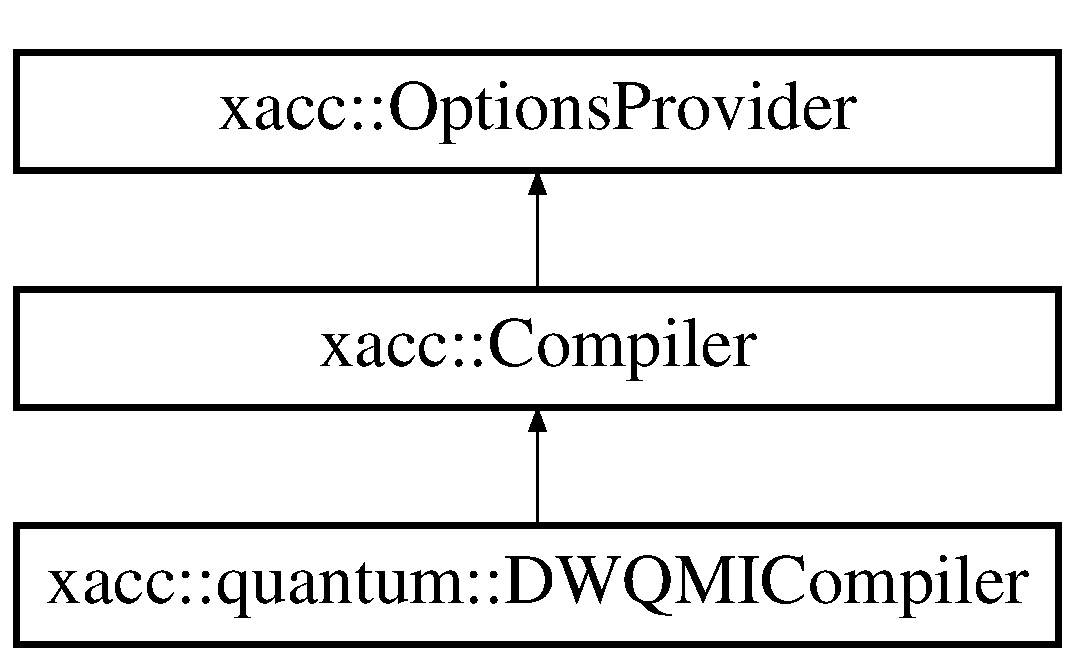
\includegraphics[height=3.000000cm]{a00034}
\end{center}
\end{figure}
\subsection*{Public Member Functions}
\begin{DoxyCompactItemize}
\item 
\hyperlink{a00034_a1f285f3eaec09363d9439676dbdfbd6a}{D\+W\+Q\+M\+I\+Compiler} ()
\item 
virtual std\+::shared\+\_\+ptr$<$ \hyperlink{a00050}{xacc\+::\+IR} $>$ \hyperlink{a00034_a0df05642f1a6fd44ce7f1c0396d50c9c}{compile} (const std\+::string \&src, std\+::shared\+\_\+ptr$<$ \hyperlink{a00011}{Accelerator} $>$ acc)
\item 
virtual std\+::shared\+\_\+ptr$<$ \hyperlink{a00050}{xacc\+::\+IR} $>$ \hyperlink{a00034_aa22591343b5509bf2c3a5820130ba906}{compile} (const std\+::string \&src)
\item 
virtual const std\+::string \hyperlink{a00034_aed42de96f8e0dd94b6de183f28aee419}{get\+Name} ()
\item 
virtual std\+::shared\+\_\+ptr$<$ options\+\_\+description $>$ \hyperlink{a00034_a0851334cc33b5b1da2694150a0a1a43c}{get\+Options} ()
\item 
virtual const std\+::string \hyperlink{a00034_a56a345539665099329209b3b5f6810c9}{translate} (const std\+::string \&buffer\+Variable, std\+::shared\+\_\+ptr$<$ \hyperlink{a00038}{Function} $>$ function)
\item 
virtual \hyperlink{a00034_a86f9135f7dc1c3246970e2a7f6540b5c}{$\sim$\+D\+W\+Q\+M\+I\+Compiler} ()
\end{DoxyCompactItemize}
\subsection*{Static Public Member Functions}
\begin{DoxyCompactItemize}
\item 
static void \hyperlink{a00034_a421daa5286f31e2b5ab4c141a34c94cd}{register\+Compiler} ()
\end{DoxyCompactItemize}
\subsection*{Additional Inherited Members}


\subsection{Detailed Description}
The \hyperlink{a00034}{D\+W\+Q\+M\+I\+Compiler} is an X\+A\+CC \hyperlink{a00023}{Compiler} that compiles D-\/\+Wave quantum machine instructions to produce an appropriate Ising form for execution on the D-\/\+Wave Q\+PU.

This compilation leverages X\+A\+CC Embedding\+Algorithms to compute the minor graph embedding represented by the input source kernel code to output the embedded Ising graph for D-\/\+Wave execution. 

\subsection{Constructor \& Destructor Documentation}
\index{xacc\+::quantum\+::\+D\+W\+Q\+M\+I\+Compiler@{xacc\+::quantum\+::\+D\+W\+Q\+M\+I\+Compiler}!D\+W\+Q\+M\+I\+Compiler@{D\+W\+Q\+M\+I\+Compiler}}
\index{D\+W\+Q\+M\+I\+Compiler@{D\+W\+Q\+M\+I\+Compiler}!xacc\+::quantum\+::\+D\+W\+Q\+M\+I\+Compiler@{xacc\+::quantum\+::\+D\+W\+Q\+M\+I\+Compiler}}
\subsubsection[{\texorpdfstring{D\+W\+Q\+M\+I\+Compiler()}{DWQMICompiler()}}]{\setlength{\rightskip}{0pt plus 5cm}xacc\+::quantum\+::\+D\+W\+Q\+M\+I\+Compiler\+::\+D\+W\+Q\+M\+I\+Compiler (
\begin{DoxyParamCaption}
{}
\end{DoxyParamCaption}
)\hspace{0.3cm}{\ttfamily [inline]}}\hypertarget{a00034_a1f285f3eaec09363d9439676dbdfbd6a}{}\label{a00034_a1f285f3eaec09363d9439676dbdfbd6a}
The \hyperlink{a00023}{Compiler}. \index{xacc\+::quantum\+::\+D\+W\+Q\+M\+I\+Compiler@{xacc\+::quantum\+::\+D\+W\+Q\+M\+I\+Compiler}!````~D\+W\+Q\+M\+I\+Compiler@{$\sim$\+D\+W\+Q\+M\+I\+Compiler}}
\index{````~D\+W\+Q\+M\+I\+Compiler@{$\sim$\+D\+W\+Q\+M\+I\+Compiler}!xacc\+::quantum\+::\+D\+W\+Q\+M\+I\+Compiler@{xacc\+::quantum\+::\+D\+W\+Q\+M\+I\+Compiler}}
\subsubsection[{\texorpdfstring{$\sim$\+D\+W\+Q\+M\+I\+Compiler()}{~DWQMICompiler()}}]{\setlength{\rightskip}{0pt plus 5cm}virtual xacc\+::quantum\+::\+D\+W\+Q\+M\+I\+Compiler\+::$\sim$\+D\+W\+Q\+M\+I\+Compiler (
\begin{DoxyParamCaption}
{}
\end{DoxyParamCaption}
)\hspace{0.3cm}{\ttfamily [inline]}, {\ttfamily [virtual]}}\hypertarget{a00034_a86f9135f7dc1c3246970e2a7f6540b5c}{}\label{a00034_a86f9135f7dc1c3246970e2a7f6540b5c}
The destructor 

\subsection{Member Function Documentation}
\index{xacc\+::quantum\+::\+D\+W\+Q\+M\+I\+Compiler@{xacc\+::quantum\+::\+D\+W\+Q\+M\+I\+Compiler}!compile@{compile}}
\index{compile@{compile}!xacc\+::quantum\+::\+D\+W\+Q\+M\+I\+Compiler@{xacc\+::quantum\+::\+D\+W\+Q\+M\+I\+Compiler}}
\subsubsection[{\texorpdfstring{compile(const std\+::string \&src, std\+::shared\+\_\+ptr$<$ Accelerator $>$ acc)}{compile(const std::string \&src, std::shared\_ptr< Accelerator > acc)}}]{\setlength{\rightskip}{0pt plus 5cm}std\+::shared\+\_\+ptr$<$ {\bf IR} $>$ xacc\+::quantum\+::\+D\+W\+Q\+M\+I\+Compiler\+::compile (
\begin{DoxyParamCaption}
\item[{const std\+::string \&}]{src, }
\item[{std\+::shared\+\_\+ptr$<$ {\bf Accelerator} $>$}]{acc}
\end{DoxyParamCaption}
)\hspace{0.3cm}{\ttfamily [virtual]}}\hypertarget{a00034_a0df05642f1a6fd44ce7f1c0396d50c9c}{}\label{a00034_a0df05642f1a6fd44ce7f1c0396d50c9c}
Compile the given kernel code for the given D-\/\+Wave \hyperlink{a00011}{Accelerator}.


\begin{DoxyParams}{Parameters}
{\em src} & The Q\+MI source code \\
\hline
{\em acc} & Reference to the D-\/\+Wave \hyperlink{a00011}{Accelerator} \\
\hline
\end{DoxyParams}
\begin{DoxyReturn}{Returns}

\end{DoxyReturn}


Implements \hyperlink{a00023_a546a40c95bb93af6a0c0ac48dbeaffc8}{xacc\+::\+Compiler}.

\index{xacc\+::quantum\+::\+D\+W\+Q\+M\+I\+Compiler@{xacc\+::quantum\+::\+D\+W\+Q\+M\+I\+Compiler}!compile@{compile}}
\index{compile@{compile}!xacc\+::quantum\+::\+D\+W\+Q\+M\+I\+Compiler@{xacc\+::quantum\+::\+D\+W\+Q\+M\+I\+Compiler}}
\subsubsection[{\texorpdfstring{compile(const std\+::string \&src)}{compile(const std::string \&src)}}]{\setlength{\rightskip}{0pt plus 5cm}std\+::shared\+\_\+ptr$<$ {\bf IR} $>$ xacc\+::quantum\+::\+D\+W\+Q\+M\+I\+Compiler\+::compile (
\begin{DoxyParamCaption}
\item[{const std\+::string \&}]{src}
\end{DoxyParamCaption}
)\hspace{0.3cm}{\ttfamily [virtual]}}\hypertarget{a00034_aa22591343b5509bf2c3a5820130ba906}{}\label{a00034_aa22591343b5509bf2c3a5820130ba906}
This method is not implemented -\/ we must always have D-\/\+Wave \hyperlink{a00011}{Accelerator} connectivity information for compilation.

\begin{DoxyReturn}{Returns}

\end{DoxyReturn}


Implements \hyperlink{a00023_a9092f5f779b570c91569b59621280c04}{xacc\+::\+Compiler}.

\index{xacc\+::quantum\+::\+D\+W\+Q\+M\+I\+Compiler@{xacc\+::quantum\+::\+D\+W\+Q\+M\+I\+Compiler}!get\+Name@{get\+Name}}
\index{get\+Name@{get\+Name}!xacc\+::quantum\+::\+D\+W\+Q\+M\+I\+Compiler@{xacc\+::quantum\+::\+D\+W\+Q\+M\+I\+Compiler}}
\subsubsection[{\texorpdfstring{get\+Name()}{getName()}}]{\setlength{\rightskip}{0pt plus 5cm}virtual const std\+::string xacc\+::quantum\+::\+D\+W\+Q\+M\+I\+Compiler\+::get\+Name (
\begin{DoxyParamCaption}
{}
\end{DoxyParamCaption}
)\hspace{0.3cm}{\ttfamily [inline]}, {\ttfamily [virtual]}}\hypertarget{a00034_aed42de96f8e0dd94b6de183f28aee419}{}\label{a00034_aed42de96f8e0dd94b6de183f28aee419}
Return the name of this \hyperlink{a00023}{Compiler} \begin{DoxyReturn}{Returns}
name \hyperlink{a00023}{Compiler} name 
\end{DoxyReturn}


Implements \hyperlink{a00023_a87fca9100e6462122f5b687c3a0fb3fb}{xacc\+::\+Compiler}.

\index{xacc\+::quantum\+::\+D\+W\+Q\+M\+I\+Compiler@{xacc\+::quantum\+::\+D\+W\+Q\+M\+I\+Compiler}!get\+Options@{get\+Options}}
\index{get\+Options@{get\+Options}!xacc\+::quantum\+::\+D\+W\+Q\+M\+I\+Compiler@{xacc\+::quantum\+::\+D\+W\+Q\+M\+I\+Compiler}}
\subsubsection[{\texorpdfstring{get\+Options()}{getOptions()}}]{\setlength{\rightskip}{0pt plus 5cm}virtual std\+::shared\+\_\+ptr$<$options\+\_\+description$>$ xacc\+::quantum\+::\+D\+W\+Q\+M\+I\+Compiler\+::get\+Options (
\begin{DoxyParamCaption}
{}
\end{DoxyParamCaption}
)\hspace{0.3cm}{\ttfamily [inline]}, {\ttfamily [virtual]}}\hypertarget{a00034_a0851334cc33b5b1da2694150a0a1a43c}{}\label{a00034_a0851334cc33b5b1da2694150a0a1a43c}
Return the command line options for this compiler

\begin{DoxyReturn}{Returns}
options Description of command line options. 
\end{DoxyReturn}


Reimplemented from \hyperlink{a00023_a9f5a8965c9c2dd895016d18264ebbe92}{xacc\+::\+Compiler}.

\index{xacc\+::quantum\+::\+D\+W\+Q\+M\+I\+Compiler@{xacc\+::quantum\+::\+D\+W\+Q\+M\+I\+Compiler}!register\+Compiler@{register\+Compiler}}
\index{register\+Compiler@{register\+Compiler}!xacc\+::quantum\+::\+D\+W\+Q\+M\+I\+Compiler@{xacc\+::quantum\+::\+D\+W\+Q\+M\+I\+Compiler}}
\subsubsection[{\texorpdfstring{register\+Compiler()}{registerCompiler()}}]{\setlength{\rightskip}{0pt plus 5cm}static void xacc\+::quantum\+::\+D\+W\+Q\+M\+I\+Compiler\+::register\+Compiler (
\begin{DoxyParamCaption}
{}
\end{DoxyParamCaption}
)\hspace{0.3cm}{\ttfamily [inline]}, {\ttfamily [static]}}\hypertarget{a00034_a421daa5286f31e2b5ab4c141a34c94cd}{}\label{a00034_a421daa5286f31e2b5ab4c141a34c94cd}
Register this \hyperlink{a00023}{Compiler} with the framework. \index{xacc\+::quantum\+::\+D\+W\+Q\+M\+I\+Compiler@{xacc\+::quantum\+::\+D\+W\+Q\+M\+I\+Compiler}!translate@{translate}}
\index{translate@{translate}!xacc\+::quantum\+::\+D\+W\+Q\+M\+I\+Compiler@{xacc\+::quantum\+::\+D\+W\+Q\+M\+I\+Compiler}}
\subsubsection[{\texorpdfstring{translate(const std\+::string \&buffer\+Variable, std\+::shared\+\_\+ptr$<$ Function $>$ function)}{translate(const std::string \&bufferVariable, std::shared\_ptr< Function > function)}}]{\setlength{\rightskip}{0pt plus 5cm}virtual const std\+::string xacc\+::quantum\+::\+D\+W\+Q\+M\+I\+Compiler\+::translate (
\begin{DoxyParamCaption}
\item[{const std\+::string \&}]{buffer\+Variable, }
\item[{std\+::shared\+\_\+ptr$<$ {\bf Function} $>$}]{function}
\end{DoxyParamCaption}
)\hspace{0.3cm}{\ttfamily [inline]}, {\ttfamily [virtual]}}\hypertarget{a00034_a56a345539665099329209b3b5f6810c9}{}\label{a00034_a56a345539665099329209b3b5f6810c9}
We don\textquotesingle{}t allow translations for the DW \hyperlink{a00023}{Compiler}. 
\begin{DoxyParams}{Parameters}
{\em buffer\+Variable} & \\
\hline
{\em function} & \\
\hline
\end{DoxyParams}
\begin{DoxyReturn}{Returns}

\end{DoxyReturn}


Implements \hyperlink{a00023_aeedbe58a33fed29e4d7694ae743e25e7}{xacc\+::\+Compiler}.



The documentation for this class was generated from the following files\+:\begin{DoxyCompactItemize}
\item 
D\+W\+Q\+M\+I\+Compiler.\+hpp\item 
D\+W\+Q\+M\+I\+Compiler.\+cpp\end{DoxyCompactItemize}

\hypertarget{a00035}{}\section{xacc\+:\+:quantum\+:\+:D\+W\+Solver Struct Reference}
\label{a00035}\index{xacc\+::quantum\+::\+D\+W\+Solver@{xacc\+::quantum\+::\+D\+W\+Solver}}


{\ttfamily \#include $<$D\+W\+Accelerator.\+hpp$>$}

\subsection*{Public Attributes}
\begin{DoxyCompactItemize}
\item 
std\+::string {\bfseries name}\hypertarget{a00035_a8a5b629dc83790a855d429c82266b772}{}\label{a00035_a8a5b629dc83790a855d429c82266b772}

\item 
std\+::string {\bfseries description}\hypertarget{a00035_a9bb9449a6ea09e11892f910a4bfd2e08}{}\label{a00035_a9bb9449a6ea09e11892f910a4bfd2e08}

\item 
double {\bfseries j\+Range\+Min}\hypertarget{a00035_a45fc23af53f44759afec0257d9878ba0}{}\label{a00035_a45fc23af53f44759afec0257d9878ba0}

\item 
double {\bfseries j\+Range\+Max}\hypertarget{a00035_aa881af1344ff55a4991c152f768ed9d6}{}\label{a00035_aa881af1344ff55a4991c152f768ed9d6}

\item 
double {\bfseries h\+Range\+Min}\hypertarget{a00035_abf475612dac8f64a7f88cfa976c393f0}{}\label{a00035_abf475612dac8f64a7f88cfa976c393f0}

\item 
double {\bfseries h\+Range\+Max}\hypertarget{a00035_a13dd875ceb06c7545fe20cde15ffac70}{}\label{a00035_a13dd875ceb06c7545fe20cde15ffac70}

\item 
int {\bfseries n\+Qubits}\hypertarget{a00035_a2908c913f5c5e3ade6551056aaadafbf}{}\label{a00035_a2908c913f5c5e3ade6551056aaadafbf}

\item 
std\+::vector$<$ std\+::pair$<$ int, int $>$ $>$ {\bfseries edges}\hypertarget{a00035_ae02cbfe68c982e50e80bcd2612c8c148}{}\label{a00035_ae02cbfe68c982e50e80bcd2612c8c148}

\end{DoxyCompactItemize}


\subsection{Detailed Description}
Wrapper for information related to the remote D-\/\+Wave solver. 

The documentation for this struct was generated from the following file\+:\begin{DoxyCompactItemize}
\item 
D\+W\+Accelerator.\+hpp\end{DoxyCompactItemize}

\hypertarget{a00036}{}\section{xacc\+:\+:quantum\+:\+:D\+W\+Vertex Class Reference}
\label{a00036}\index{xacc\+::quantum\+::\+D\+W\+Vertex@{xacc\+::quantum\+::\+D\+W\+Vertex}}


{\ttfamily \#include $<$D\+W\+Graph.\+hpp$>$}

Inheritance diagram for xacc\+:\+:quantum\+:\+:D\+W\+Vertex\+:\begin{figure}[H]
\begin{center}
\leavevmode
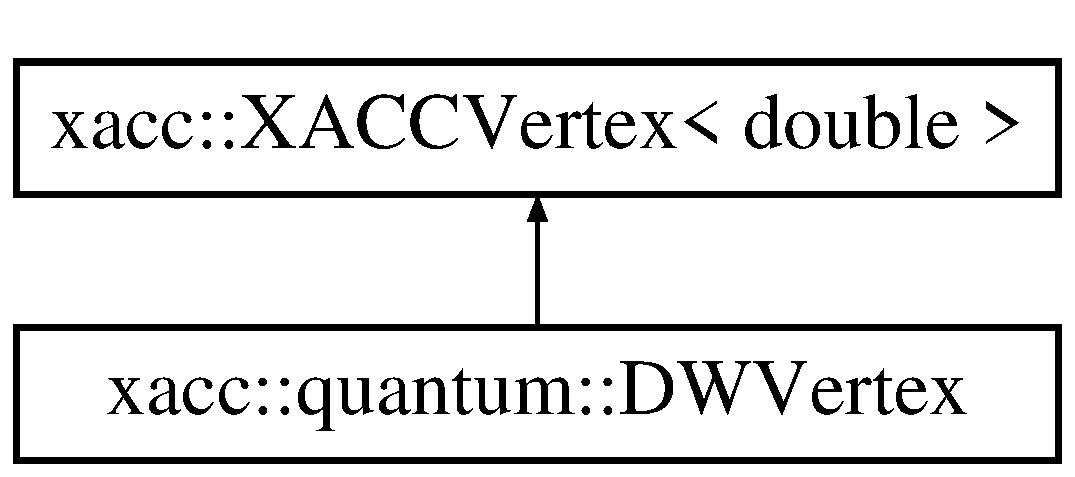
\includegraphics[height=2.000000cm]{a00036}
\end{center}
\end{figure}
\subsection*{Additional Inherited Members}


\subsection{Detailed Description}
The \hyperlink{a00036}{D\+W\+Vertex} is a subclass of the \hyperlink{a00085}{X\+A\+C\+C\+Vertex} that keeps track of one vertex parameter -\/ the qubit bias parameter. \hyperlink{a00085}{X\+A\+C\+C\+Vertex} already keeps track of edge weights. 

The documentation for this class was generated from the following file\+:\begin{DoxyCompactItemize}
\item 
D\+W\+Graph.\+hpp\end{DoxyCompactItemize}

\hypertarget{a00037}{}\section{xacc\+:\+:quantum\+:\+:Embedding\+Algorithm Class Reference}
\label{a00037}\index{xacc\+::quantum\+::\+Embedding\+Algorithm@{xacc\+::quantum\+::\+Embedding\+Algorithm}}


{\ttfamily \#include $<$Embedding\+Algorithm.\+hpp$>$}

Inheritance diagram for xacc\+:\+:quantum\+:\+:Embedding\+Algorithm\+:\begin{figure}[H]
\begin{center}
\leavevmode
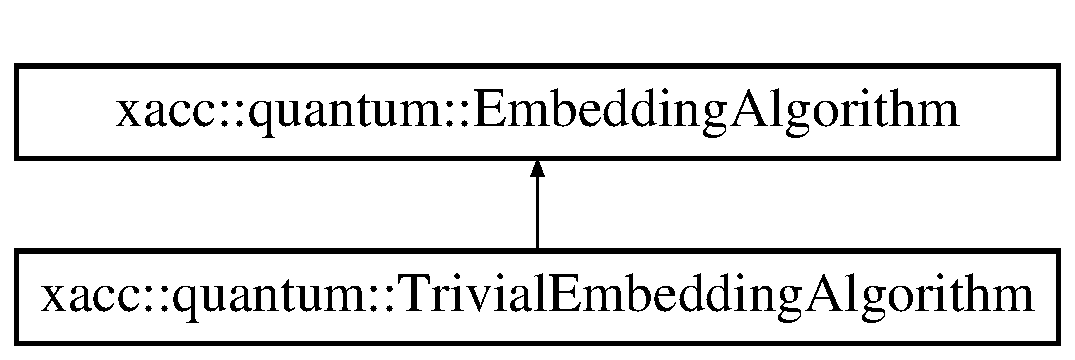
\includegraphics[height=2.000000cm]{a00037}
\end{center}
\end{figure}
\subsection*{Public Member Functions}
\begin{DoxyCompactItemize}
\item 
\hyperlink{a00037_abad06507eef6b63af0884e3a96145c69}{Embedding\+Algorithm} ()
\item 
virtual \hyperlink{a00037_aa43660ad5d4c4b3ac67863892c33dc51}{$\sim$\+Embedding\+Algorithm} ()
\item 
virtual std\+::map$<$ int, std\+::list$<$ int $>$ $>$ \hyperlink{a00037_a6fca277e217884ff79802770189276fe}{embed} (std\+::shared\+\_\+ptr$<$ \hyperlink{a00030}{D\+W\+Graph} $>$ problem, std\+::shared\+\_\+ptr$<$ \hyperlink{a00043}{Accelerator\+Graph} $>$ hardware, std\+::map$<$ std\+::string, std\+::string $>$ params=std\+::map$<$ std\+::string, std\+::string $>$())=0
\item 
virtual std\+::string \hyperlink{a00037_a21079dc8ee37792977f5fd209e3f3b19}{name} ()=0
\end{DoxyCompactItemize}


\subsection{Detailed Description}
The \hyperlink{a00037}{Embedding\+Algorithm} class provides an interface for minor graph embedding algorithms. 

\subsection{Constructor \& Destructor Documentation}
\index{xacc\+::quantum\+::\+Embedding\+Algorithm@{xacc\+::quantum\+::\+Embedding\+Algorithm}!Embedding\+Algorithm@{Embedding\+Algorithm}}
\index{Embedding\+Algorithm@{Embedding\+Algorithm}!xacc\+::quantum\+::\+Embedding\+Algorithm@{xacc\+::quantum\+::\+Embedding\+Algorithm}}
\subsubsection[{\texorpdfstring{Embedding\+Algorithm()}{EmbeddingAlgorithm()}}]{\setlength{\rightskip}{0pt plus 5cm}xacc\+::quantum\+::\+Embedding\+Algorithm\+::\+Embedding\+Algorithm (
\begin{DoxyParamCaption}
{}
\end{DoxyParamCaption}
)\hspace{0.3cm}{\ttfamily [inline]}}\hypertarget{a00037_abad06507eef6b63af0884e3a96145c69}{}\label{a00037_abad06507eef6b63af0884e3a96145c69}
The Constructor \index{xacc\+::quantum\+::\+Embedding\+Algorithm@{xacc\+::quantum\+::\+Embedding\+Algorithm}!````~Embedding\+Algorithm@{$\sim$\+Embedding\+Algorithm}}
\index{````~Embedding\+Algorithm@{$\sim$\+Embedding\+Algorithm}!xacc\+::quantum\+::\+Embedding\+Algorithm@{xacc\+::quantum\+::\+Embedding\+Algorithm}}
\subsubsection[{\texorpdfstring{$\sim$\+Embedding\+Algorithm()}{~EmbeddingAlgorithm()}}]{\setlength{\rightskip}{0pt plus 5cm}virtual xacc\+::quantum\+::\+Embedding\+Algorithm\+::$\sim$\+Embedding\+Algorithm (
\begin{DoxyParamCaption}
{}
\end{DoxyParamCaption}
)\hspace{0.3cm}{\ttfamily [inline]}, {\ttfamily [virtual]}}\hypertarget{a00037_aa43660ad5d4c4b3ac67863892c33dc51}{}\label{a00037_aa43660ad5d4c4b3ac67863892c33dc51}
The Destructor 

\subsection{Member Function Documentation}
\index{xacc\+::quantum\+::\+Embedding\+Algorithm@{xacc\+::quantum\+::\+Embedding\+Algorithm}!embed@{embed}}
\index{embed@{embed}!xacc\+::quantum\+::\+Embedding\+Algorithm@{xacc\+::quantum\+::\+Embedding\+Algorithm}}
\subsubsection[{\texorpdfstring{embed(std\+::shared\+\_\+ptr$<$ D\+W\+Graph $>$ problem, std\+::shared\+\_\+ptr$<$ Accelerator\+Graph $>$ hardware, std\+::map$<$ std\+::string, std\+::string $>$ params=std\+::map$<$ std\+::string, std\+::string $>$())=0}{embed(std::shared\_ptr< DWGraph > problem, std::shared\_ptr< AcceleratorGraph > hardware, std::map< std::string, std::string > params=std::map< std::string, std::string >())=0}}]{\setlength{\rightskip}{0pt plus 5cm}virtual std\+::map$<$int, std\+::list$<$int$>$ $>$ xacc\+::quantum\+::\+Embedding\+Algorithm\+::embed (
\begin{DoxyParamCaption}
\item[{std\+::shared\+\_\+ptr$<$ {\bf D\+W\+Graph} $>$}]{problem, }
\item[{std\+::shared\+\_\+ptr$<$ {\bf Accelerator\+Graph} $>$}]{hardware, }
\item[{std\+::map$<$ std\+::string, std\+::string $>$}]{params = {\ttfamily std\+:\+:map$<$~std\+:\+:string,~std\+:\+:string~$>$()}}
\end{DoxyParamCaption}
)\hspace{0.3cm}{\ttfamily [pure virtual]}}\hypertarget{a00037_a6fca277e217884ff79802770189276fe}{}\label{a00037_a6fca277e217884ff79802770189276fe}
Implementations of \hyperlink{a00037}{Embedding\+Algorithm} implement this method to provide a valid minor graph embedding of the given problem graph into the given hardware graph.


\begin{DoxyParams}{Parameters}
{\em problem} & The problem graph to be embedded into the hardware graph \\
\hline
{\em hardware} & The hardware graph. \\
\hline
{\em params} & Any key-\/value string parameters to influence the algorithm. \\
\hline
\end{DoxyParams}
\begin{DoxyReturn}{Returns}
embedding A mapping of problem vertex indices to the list of hardware vertices they map to 
\end{DoxyReturn}


Implemented in \hyperlink{a00083_a09e162a745528ffa3ea847dd5afee45b}{xacc\+::quantum\+::\+Trivial\+Embedding\+Algorithm}.

\index{xacc\+::quantum\+::\+Embedding\+Algorithm@{xacc\+::quantum\+::\+Embedding\+Algorithm}!name@{name}}
\index{name@{name}!xacc\+::quantum\+::\+Embedding\+Algorithm@{xacc\+::quantum\+::\+Embedding\+Algorithm}}
\subsubsection[{\texorpdfstring{name()=0}{name()=0}}]{\setlength{\rightskip}{0pt plus 5cm}virtual std\+::string xacc\+::quantum\+::\+Embedding\+Algorithm\+::name (
\begin{DoxyParamCaption}
{}
\end{DoxyParamCaption}
)\hspace{0.3cm}{\ttfamily [pure virtual]}}\hypertarget{a00037_a21079dc8ee37792977f5fd209e3f3b19}{}\label{a00037_a21079dc8ee37792977f5fd209e3f3b19}
Return the name of this Embedding Algorithm \begin{DoxyReturn}{Returns}

\end{DoxyReturn}


Implemented in \hyperlink{a00083_a5d3e8c56b53cda9c682dedc534bf38fb}{xacc\+::quantum\+::\+Trivial\+Embedding\+Algorithm}.



The documentation for this class was generated from the following file\+:\begin{DoxyCompactItemize}
\item 
Embedding\+Algorithm.\+hpp\end{DoxyCompactItemize}

\hypertarget{a00038}{}\section{xacc\+:\+:Function Class Reference}
\label{a00038}\index{xacc\+::\+Function@{xacc\+::\+Function}}


{\ttfamily \#include $<$Function.\+hpp$>$}

Inheritance diagram for xacc\+:\+:Function\+:\begin{figure}[H]
\begin{center}
\leavevmode
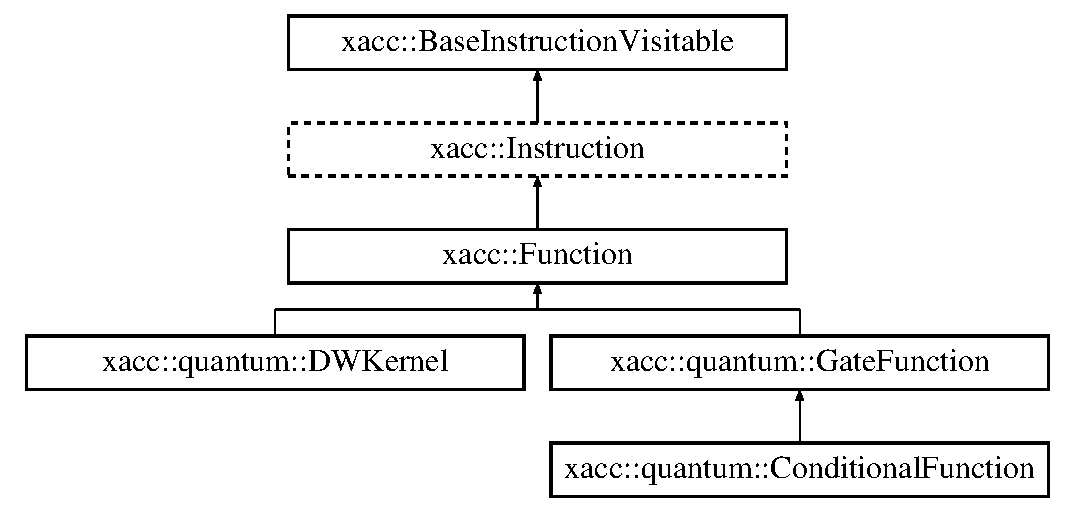
\includegraphics[height=5.000000cm]{a00038}
\end{center}
\end{figure}
\subsection*{Public Member Functions}
\begin{DoxyCompactItemize}
\item 
virtual const int \hyperlink{a00038_a8901985525f59713e14c61713e07c086}{n\+Instructions} ()=0
\item 
virtual Inst\+Ptr \hyperlink{a00038_afa549fc91b5a05f26d8139954a7e0ed5}{get\+Instruction} (const int idx)=0
\item 
virtual std\+::list$<$ Inst\+Ptr $>$ \hyperlink{a00038_aaf80bd3d49113a92b520785572663032}{get\+Instructions} ()=0
\item 
virtual void \hyperlink{a00038_ab6478b09bb28e194bb555b3180737733}{remove\+Instruction} (const int idx)=0
\item 
virtual void \hyperlink{a00038_a2ef6a4923a6734f90f6ee3d94d263af0}{replace\+Instruction} (const int idx, Inst\+Ptr new\+Inst)=0
\item 
virtual void \hyperlink{a00038_acde702e44bdbc2759b338365218d7ebe}{insert\+Instruction} (const int idx, Inst\+Ptr new\+Inst)=0
\item 
virtual void \hyperlink{a00038_aa8c9ec2d08be75c69399d4254b0216f5}{add\+Instruction} (Inst\+Ptr instruction)=0
\item 
virtual bool \hyperlink{a00038_aa75500c657b5c3e0e36213e1506aad97}{is\+Composite} ()
\item 
virtual void \hyperlink{a00038_af6ae9453027789a2aaec30e59c9e45e3}{evaluate\+Variable\+Parameters} (std\+::vector$<$ Instruction\+Parameter $>$ parameters)=0
\item 
virtual \hyperlink{a00038_a04b25ba4da1ddfa4ec4ec6d6ffb25bc3}{$\sim$\+Function} ()
\end{DoxyCompactItemize}
\subsection*{Additional Inherited Members}


\subsection{Detailed Description}
The \hyperlink{a00038}{Function} is an \hyperlink{a00046}{Instruction} that contains further child Instructions.

\begin{DoxyAuthor}{Author}
Alex Mc\+Caskey 
\end{DoxyAuthor}


\subsection{Constructor \& Destructor Documentation}
\index{xacc\+::\+Function@{xacc\+::\+Function}!````~Function@{$\sim$\+Function}}
\index{````~Function@{$\sim$\+Function}!xacc\+::\+Function@{xacc\+::\+Function}}
\subsubsection[{\texorpdfstring{$\sim$\+Function()}{~Function()}}]{\setlength{\rightskip}{0pt plus 5cm}virtual xacc\+::\+Function\+::$\sim$\+Function (
\begin{DoxyParamCaption}
{}
\end{DoxyParamCaption}
)\hspace{0.3cm}{\ttfamily [inline]}, {\ttfamily [virtual]}}\hypertarget{a00038_a04b25ba4da1ddfa4ec4ec6d6ffb25bc3}{}\label{a00038_a04b25ba4da1ddfa4ec4ec6d6ffb25bc3}
The destructor 

\subsection{Member Function Documentation}
\index{xacc\+::\+Function@{xacc\+::\+Function}!add\+Instruction@{add\+Instruction}}
\index{add\+Instruction@{add\+Instruction}!xacc\+::\+Function@{xacc\+::\+Function}}
\subsubsection[{\texorpdfstring{add\+Instruction(\+Inst\+Ptr instruction)=0}{addInstruction(InstPtr instruction)=0}}]{\setlength{\rightskip}{0pt plus 5cm}virtual void xacc\+::\+Function\+::add\+Instruction (
\begin{DoxyParamCaption}
\item[{Inst\+Ptr}]{instruction}
\end{DoxyParamCaption}
)\hspace{0.3cm}{\ttfamily [pure virtual]}}\hypertarget{a00038_aa8c9ec2d08be75c69399d4254b0216f5}{}\label{a00038_aa8c9ec2d08be75c69399d4254b0216f5}
Add an \hyperlink{a00046}{Instruction} to this \hyperlink{a00038}{Function}.


\begin{DoxyParams}{Parameters}
{\em instruction} & The instruction to add. \\
\hline
\end{DoxyParams}


Implemented in \hyperlink{a00040_a892fb69a10f0a7cb5abdab4cca61b80a}{xacc\+::quantum\+::\+Gate\+Function}, \hyperlink{a00032_a4c3043d6971999c3a09e797fc55deb6c}{xacc\+::quantum\+::\+D\+W\+Kernel}, and \hyperlink{a00025_a6aedad20f96390880efdc0a476b3273f}{xacc\+::quantum\+::\+Conditional\+Function}.

\index{xacc\+::\+Function@{xacc\+::\+Function}!evaluate\+Variable\+Parameters@{evaluate\+Variable\+Parameters}}
\index{evaluate\+Variable\+Parameters@{evaluate\+Variable\+Parameters}!xacc\+::\+Function@{xacc\+::\+Function}}
\subsubsection[{\texorpdfstring{evaluate\+Variable\+Parameters(std\+::vector$<$ Instruction\+Parameter $>$ parameters)=0}{evaluateVariableParameters(std::vector< InstructionParameter > parameters)=0}}]{\setlength{\rightskip}{0pt plus 5cm}virtual void xacc\+::\+Function\+::evaluate\+Variable\+Parameters (
\begin{DoxyParamCaption}
\item[{std\+::vector$<$ Instruction\+Parameter $>$}]{parameters}
\end{DoxyParamCaption}
)\hspace{0.3cm}{\ttfamily [pure virtual]}}\hypertarget{a00038_af6ae9453027789a2aaec30e59c9e45e3}{}\label{a00038_af6ae9453027789a2aaec30e59c9e45e3}
This method is used to evaluate this \hyperlink{a00038}{Function}\textquotesingle{}s parameterized Instructions that have string variable Instruction\+Parameters. These parameters are updated with the given runtime parameters.


\begin{DoxyParams}{Parameters}
{\em parameters} & The runtime parameters \\
\hline
\end{DoxyParams}


Implemented in \hyperlink{a00040_a4bcbd2c8c4b615d74e4a4d39952fd411}{xacc\+::quantum\+::\+Gate\+Function}, and \hyperlink{a00032_a09ffac417d4ecbbd82d7a680ad8dfcce}{xacc\+::quantum\+::\+D\+W\+Kernel}.

\index{xacc\+::\+Function@{xacc\+::\+Function}!get\+Instruction@{get\+Instruction}}
\index{get\+Instruction@{get\+Instruction}!xacc\+::\+Function@{xacc\+::\+Function}}
\subsubsection[{\texorpdfstring{get\+Instruction(const int idx)=0}{getInstruction(const int idx)=0}}]{\setlength{\rightskip}{0pt plus 5cm}virtual Inst\+Ptr xacc\+::\+Function\+::get\+Instruction (
\begin{DoxyParamCaption}
\item[{const int}]{idx}
\end{DoxyParamCaption}
)\hspace{0.3cm}{\ttfamily [pure virtual]}}\hypertarget{a00038_afa549fc91b5a05f26d8139954a7e0ed5}{}\label{a00038_afa549fc91b5a05f26d8139954a7e0ed5}
Return the \hyperlink{a00046}{Instruction} at the given index.


\begin{DoxyParams}{Parameters}
{\em idx} & The desired \hyperlink{a00046}{Instruction} index \\
\hline
\end{DoxyParams}
\begin{DoxyReturn}{Returns}
inst The instruction at the given index. 
\end{DoxyReturn}


Implemented in \hyperlink{a00040_a841d656eed8aa9b4c0eec3f1da38069c}{xacc\+::quantum\+::\+Gate\+Function}, and \hyperlink{a00032_a00f23cd2e15ea6b9d00d4f3dbe1540f8}{xacc\+::quantum\+::\+D\+W\+Kernel}.

\index{xacc\+::\+Function@{xacc\+::\+Function}!get\+Instructions@{get\+Instructions}}
\index{get\+Instructions@{get\+Instructions}!xacc\+::\+Function@{xacc\+::\+Function}}
\subsubsection[{\texorpdfstring{get\+Instructions()=0}{getInstructions()=0}}]{\setlength{\rightskip}{0pt plus 5cm}virtual std\+::list$<$Inst\+Ptr$>$ xacc\+::\+Function\+::get\+Instructions (
\begin{DoxyParamCaption}
{}
\end{DoxyParamCaption}
)\hspace{0.3cm}{\ttfamily [pure virtual]}}\hypertarget{a00038_aaf80bd3d49113a92b520785572663032}{}\label{a00038_aaf80bd3d49113a92b520785572663032}
Return all Instructions in this \hyperlink{a00038}{Function}

\begin{DoxyReturn}{Returns}
insts The list of this \hyperlink{a00038}{Function}\textquotesingle{}s Instructions 
\end{DoxyReturn}


Implemented in \hyperlink{a00040_aebce6a9e64aed7f4aff86df752bacfe2}{xacc\+::quantum\+::\+Gate\+Function}, and \hyperlink{a00032_abbb8f2b1c78623c377524e45d581d018}{xacc\+::quantum\+::\+D\+W\+Kernel}.

\index{xacc\+::\+Function@{xacc\+::\+Function}!insert\+Instruction@{insert\+Instruction}}
\index{insert\+Instruction@{insert\+Instruction}!xacc\+::\+Function@{xacc\+::\+Function}}
\subsubsection[{\texorpdfstring{insert\+Instruction(const int idx, Inst\+Ptr new\+Inst)=0}{insertInstruction(const int idx, InstPtr newInst)=0}}]{\setlength{\rightskip}{0pt plus 5cm}virtual void xacc\+::\+Function\+::insert\+Instruction (
\begin{DoxyParamCaption}
\item[{const int}]{idx, }
\item[{Inst\+Ptr}]{new\+Inst}
\end{DoxyParamCaption}
)\hspace{0.3cm}{\ttfamily [pure virtual]}}\hypertarget{a00038_acde702e44bdbc2759b338365218d7ebe}{}\label{a00038_acde702e44bdbc2759b338365218d7ebe}
Insert a new \hyperlink{a00046}{Instruction} at the given index. All previous instructions are pushed back, ie their new indices are current\+Index + 1.


\begin{DoxyParams}{Parameters}
{\em idx} & The index where the new instruction should be inserted \\
\hline
{\em new\+Inst} & The new \hyperlink{a00046}{Instruction} to insert. \\
\hline
\end{DoxyParams}


Implemented in \hyperlink{a00040_aed3b963f1c4eb3215ca46af48d78f588}{xacc\+::quantum\+::\+Gate\+Function}, and \hyperlink{a00032_a1627af0141f70fc4a3cd500a13fb31b8}{xacc\+::quantum\+::\+D\+W\+Kernel}.

\index{xacc\+::\+Function@{xacc\+::\+Function}!is\+Composite@{is\+Composite}}
\index{is\+Composite@{is\+Composite}!xacc\+::\+Function@{xacc\+::\+Function}}
\subsubsection[{\texorpdfstring{is\+Composite()}{isComposite()}}]{\setlength{\rightskip}{0pt plus 5cm}virtual bool xacc\+::\+Function\+::is\+Composite (
\begin{DoxyParamCaption}
{}
\end{DoxyParamCaption}
)\hspace{0.3cm}{\ttfamily [inline]}, {\ttfamily [virtual]}}\hypertarget{a00038_aa75500c657b5c3e0e36213e1506aad97}{}\label{a00038_aa75500c657b5c3e0e36213e1506aad97}
Return true always to indicate that the \hyperlink{a00038}{Function} is composite.

\begin{DoxyReturn}{Returns}
composite True indicating this is a composite \hyperlink{a00046}{Instruction}. 
\end{DoxyReturn}


Reimplemented from \hyperlink{a00046_a4383f1036d0fcfe890ab9c613dbd5f38}{xacc\+::\+Instruction}.

\index{xacc\+::\+Function@{xacc\+::\+Function}!n\+Instructions@{n\+Instructions}}
\index{n\+Instructions@{n\+Instructions}!xacc\+::\+Function@{xacc\+::\+Function}}
\subsubsection[{\texorpdfstring{n\+Instructions()=0}{nInstructions()=0}}]{\setlength{\rightskip}{0pt plus 5cm}virtual const int xacc\+::\+Function\+::n\+Instructions (
\begin{DoxyParamCaption}
{}
\end{DoxyParamCaption}
)\hspace{0.3cm}{\ttfamily [pure virtual]}}\hypertarget{a00038_a8901985525f59713e14c61713e07c086}{}\label{a00038_a8901985525f59713e14c61713e07c086}
Return the number of Instructions that this \hyperlink{a00038}{Function} contains.

\begin{DoxyReturn}{Returns}
n\+Inst The number of instructions 
\end{DoxyReturn}


Implemented in \hyperlink{a00040_aa70b26156c060fec71316fe5e98bb102}{xacc\+::quantum\+::\+Gate\+Function}, and \hyperlink{a00032_a79aecc7419a20b8779372ef36fc24806}{xacc\+::quantum\+::\+D\+W\+Kernel}.

\index{xacc\+::\+Function@{xacc\+::\+Function}!remove\+Instruction@{remove\+Instruction}}
\index{remove\+Instruction@{remove\+Instruction}!xacc\+::\+Function@{xacc\+::\+Function}}
\subsubsection[{\texorpdfstring{remove\+Instruction(const int idx)=0}{removeInstruction(const int idx)=0}}]{\setlength{\rightskip}{0pt plus 5cm}virtual void xacc\+::\+Function\+::remove\+Instruction (
\begin{DoxyParamCaption}
\item[{const int}]{idx}
\end{DoxyParamCaption}
)\hspace{0.3cm}{\ttfamily [pure virtual]}}\hypertarget{a00038_ab6478b09bb28e194bb555b3180737733}{}\label{a00038_ab6478b09bb28e194bb555b3180737733}
Remove the \hyperlink{a00046}{Instruction} at the given index.


\begin{DoxyParams}{Parameters}
{\em idx} & The index of the \hyperlink{a00046}{Instruction} to remove. \\
\hline
\end{DoxyParams}


Implemented in \hyperlink{a00040_a44ca35d081577de9ad2930f93c01e89d}{xacc\+::quantum\+::\+Gate\+Function}, and \hyperlink{a00032_af2bcfd679e6cb89194f3f0bff8622b99}{xacc\+::quantum\+::\+D\+W\+Kernel}.

\index{xacc\+::\+Function@{xacc\+::\+Function}!replace\+Instruction@{replace\+Instruction}}
\index{replace\+Instruction@{replace\+Instruction}!xacc\+::\+Function@{xacc\+::\+Function}}
\subsubsection[{\texorpdfstring{replace\+Instruction(const int idx, Inst\+Ptr new\+Inst)=0}{replaceInstruction(const int idx, InstPtr newInst)=0}}]{\setlength{\rightskip}{0pt plus 5cm}virtual void xacc\+::\+Function\+::replace\+Instruction (
\begin{DoxyParamCaption}
\item[{const int}]{idx, }
\item[{Inst\+Ptr}]{new\+Inst}
\end{DoxyParamCaption}
)\hspace{0.3cm}{\ttfamily [pure virtual]}}\hypertarget{a00038_a2ef6a4923a6734f90f6ee3d94d263af0}{}\label{a00038_a2ef6a4923a6734f90f6ee3d94d263af0}
Replace the \hyperlink{a00046}{Instruction} at the given index with the given new \hyperlink{a00046}{Instruction}.


\begin{DoxyParams}{Parameters}
{\em idx} & The index of the \hyperlink{a00046}{Instruction} to replace. \\
\hline
{\em new\+Inst} & The new \hyperlink{a00046}{Instruction} to replace with. \\
\hline
\end{DoxyParams}


Implemented in \hyperlink{a00040_a182fdfabbf546ae89e4f2384bafb45c9}{xacc\+::quantum\+::\+Gate\+Function}, and \hyperlink{a00032_a75eb3560d2f81c9a5ae1cf765deb0e83}{xacc\+::quantum\+::\+D\+W\+Kernel}.



The documentation for this class was generated from the following file\+:\begin{DoxyCompactItemize}
\item 
Function.\+hpp\end{DoxyCompactItemize}

\hypertarget{a00039}{}\section{xacc\+:\+:quantum\+:\+:Functional\+Gate\+Instruction\+Visitor Class Reference}
\label{a00039}\index{xacc\+::quantum\+::\+Functional\+Gate\+Instruction\+Visitor@{xacc\+::quantum\+::\+Functional\+Gate\+Instruction\+Visitor}}
Inheritance diagram for xacc\+:\+:quantum\+:\+:Functional\+Gate\+Instruction\+Visitor\+:\begin{figure}[H]
\begin{center}
\leavevmode
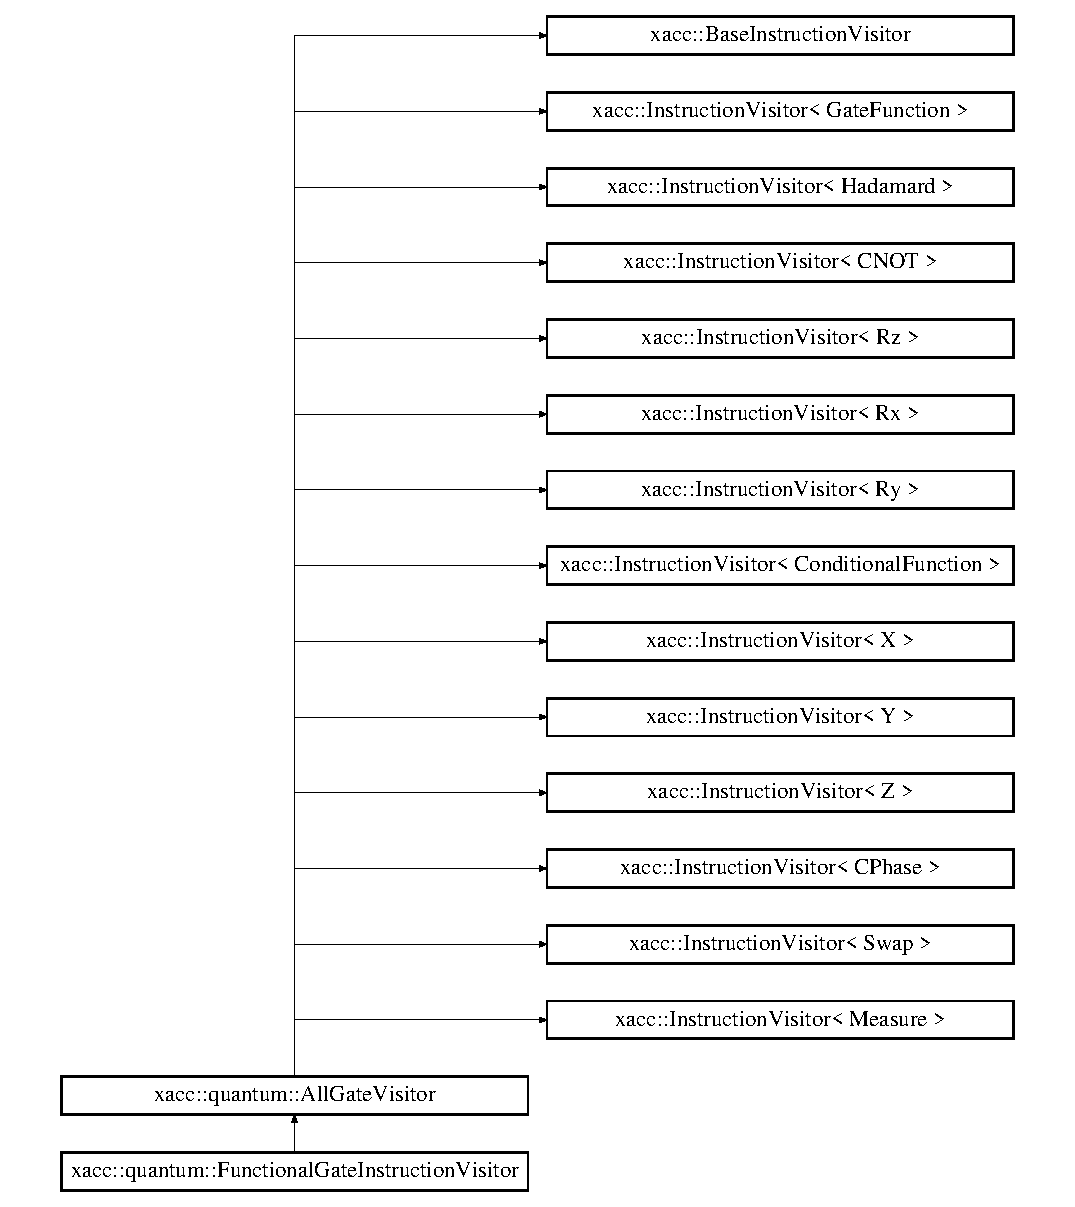
\includegraphics[height=12.000000cm]{a00039}
\end{center}
\end{figure}
\subsection*{Public Member Functions}
\begin{DoxyCompactItemize}
\item 
{\footnotesize template$<$typename HF , typename C\+NF , typename XF , typename YF , typename ZF , typename R\+XF , typename R\+YF , typename R\+ZF , typename MF , typename CF , typename C\+PF , typename S\+W\+A\+PF $>$ }\\{\bfseries Functional\+Gate\+Instruction\+Visitor} (HF h, C\+NF cn, XF x, YF y, ZF z, R\+XF rx, R\+YF ry, R\+ZF rz, MF m, CF c, C\+PF cp, S\+W\+A\+PF sw)\hypertarget{a00039_a4e3c27cd6b1acf063967b7b09a1eca09}{}\label{a00039_a4e3c27cd6b1acf063967b7b09a1eca09}

\item 
void {\bfseries visit} (\hyperlink{a00044}{Hadamard} \&h)\hypertarget{a00039_ac5245d34429dc112e7cd0e371108fcb5}{}\label{a00039_ac5245d34429dc112e7cd0e371108fcb5}

\item 
void {\bfseries visit} (\hyperlink{a00022}{C\+N\+OT} \&cn)\hypertarget{a00039_ad4eddafe8ca3906cd4aa5b98087a789a}{}\label{a00039_ad4eddafe8ca3906cd4aa5b98087a789a}

\item 
void {\bfseries visit} (\hyperlink{a00084}{X} \&x)\hypertarget{a00039_ac5d184daee7e755c9ede67b34bc2d091}{}\label{a00039_ac5d184daee7e755c9ede67b34bc2d091}

\item 
void {\bfseries visit} (\hyperlink{a00087}{Y} \&y)\hypertarget{a00039_a11dfa753a155346a45d7116a78c8f39f}{}\label{a00039_a11dfa753a155346a45d7116a78c8f39f}

\item 
void {\bfseries visit} (\hyperlink{a00088}{Z} \&z)\hypertarget{a00039_a4baf19da581fa9875739a227aba9cf60}{}\label{a00039_a4baf19da581fa9875739a227aba9cf60}

\item 
void {\bfseries visit} (\hyperlink{a00055}{Measure} \&m)\hypertarget{a00039_ad946faf8e2b6eff3e9e142907ec8e05a}{}\label{a00039_ad946faf8e2b6eff3e9e142907ec8e05a}

\item 
void {\bfseries visit} (\hyperlink{a00025}{Conditional\+Function} \&c)\hypertarget{a00039_a5cdb38902c241e7ae672a2631f1d61f3}{}\label{a00039_a5cdb38902c241e7ae672a2631f1d61f3}

\item 
void {\bfseries visit} (\hyperlink{a00073}{Rx} \&rx)\hypertarget{a00039_a6eb99e4b488773c750b7d9734ac1e885}{}\label{a00039_a6eb99e4b488773c750b7d9734ac1e885}

\item 
void {\bfseries visit} (\hyperlink{a00074}{Ry} \&ry)\hypertarget{a00039_aa22aad7b316386f5ef35672337c05ffc}{}\label{a00039_aa22aad7b316386f5ef35672337c05ffc}

\item 
void {\bfseries visit} (\hyperlink{a00027}{C\+Phase} \&cp)\hypertarget{a00039_a5475eece7afe380512a1a0215b92d302}{}\label{a00039_a5475eece7afe380512a1a0215b92d302}

\item 
void {\bfseries visit} (\hyperlink{a00075}{Rz} \&rz)\hypertarget{a00039_a8857ecf8f8f1b6143da8f31a722fe03e}{}\label{a00039_a8857ecf8f8f1b6143da8f31a722fe03e}

\item 
void {\bfseries visit} (\hyperlink{a00040}{Gate\+Function} \&f)\hypertarget{a00039_ad7d15225cf258fe59660ba828baff357}{}\label{a00039_ad7d15225cf258fe59660ba828baff357}

\item 
void {\bfseries visit} (\hyperlink{a00082}{Swap} \&s)\hypertarget{a00039_a30f46be43607813996c9cc090c1a5a16}{}\label{a00039_a30f46be43607813996c9cc090c1a5a16}

\end{DoxyCompactItemize}
\subsection*{Protected Attributes}
\begin{DoxyCompactItemize}
\item 
std\+::function$<$ void(\hyperlink{a00044}{Hadamard} \&)$>$ {\bfseries h\+Action}\hypertarget{a00039_a02f1401c9b0d1da801027f3bc0b5227e}{}\label{a00039_a02f1401c9b0d1da801027f3bc0b5227e}

\item 
std\+::function$<$ void(\hyperlink{a00022}{C\+N\+OT} \&)$>$ {\bfseries cnot\+Action}\hypertarget{a00039_a4d6bd8c2fd1af775ed08946942f60a0b}{}\label{a00039_a4d6bd8c2fd1af775ed08946942f60a0b}

\item 
std\+::function$<$ void(\hyperlink{a00084}{X} \&)$>$ {\bfseries x\+Action}\hypertarget{a00039_a9e0295434a2224b776609b057147a9af}{}\label{a00039_a9e0295434a2224b776609b057147a9af}

\item 
std\+::function$<$ void(\hyperlink{a00087}{Y} \&)$>$ {\bfseries y\+Action}\hypertarget{a00039_ae78f91a5cc9a7006f6bb1acee1c00501}{}\label{a00039_ae78f91a5cc9a7006f6bb1acee1c00501}

\item 
std\+::function$<$ void(\hyperlink{a00088}{Z} \&)$>$ {\bfseries z\+Action}\hypertarget{a00039_ae197f358e3d0777feb3656455e2ee672}{}\label{a00039_ae197f358e3d0777feb3656455e2ee672}

\item 
std\+::function$<$ void(\hyperlink{a00055}{Measure} \&)$>$ {\bfseries measure\+Action}\hypertarget{a00039_a239748abedd67c7b30cad12e545d1926}{}\label{a00039_a239748abedd67c7b30cad12e545d1926}

\item 
std\+::function$<$ void(\hyperlink{a00025}{Conditional\+Function} \&)$>$ {\bfseries cond\+Action}\hypertarget{a00039_a5c0595a70b1f7ae50f3e29a985e249e9}{}\label{a00039_a5c0595a70b1f7ae50f3e29a985e249e9}

\item 
std\+::function$<$ void(\hyperlink{a00073}{Rx} \&)$>$ {\bfseries rx\+Action}\hypertarget{a00039_ab79bb3eb3050d1c599061863bb2e219e}{}\label{a00039_ab79bb3eb3050d1c599061863bb2e219e}

\item 
std\+::function$<$ void(\hyperlink{a00074}{Ry} \&)$>$ {\bfseries ry\+Action}\hypertarget{a00039_a229b7d9aae52638c6eff04bd16bb9973}{}\label{a00039_a229b7d9aae52638c6eff04bd16bb9973}

\item 
std\+::function$<$ void(\hyperlink{a00075}{Rz} \&)$>$ {\bfseries rz\+Action}\hypertarget{a00039_a586ab5721150c67ad3ced46e2a236b44}{}\label{a00039_a586ab5721150c67ad3ced46e2a236b44}

\item 
std\+::function$<$ void(\hyperlink{a00027}{C\+Phase} \&)$>$ {\bfseries cp\+Action}\hypertarget{a00039_a5b88a0c9789e7b6d44527b2df6819ac5}{}\label{a00039_a5b88a0c9789e7b6d44527b2df6819ac5}

\item 
std\+::function$<$ void(\hyperlink{a00082}{Swap} \&)$>$ {\bfseries sw\+Action}\hypertarget{a00039_a5060cd4c2b1b259e32bda0e7ecc78e85}{}\label{a00039_a5060cd4c2b1b259e32bda0e7ecc78e85}

\end{DoxyCompactItemize}


The documentation for this class was generated from the following file\+:\begin{DoxyCompactItemize}
\item 
Functional\+Gate\+Instruction\+Visitor.\+hpp\end{DoxyCompactItemize}

\hypertarget{a00040}{}\section{xacc\+:\+:quantum\+:\+:Gate\+Function Class Reference}
\label{a00040}\index{xacc\+::quantum\+::\+Gate\+Function@{xacc\+::quantum\+::\+Gate\+Function}}


{\ttfamily \#include $<$Gate\+Function.\+hpp$>$}

Inheritance diagram for xacc\+:\+:quantum\+:\+:Gate\+Function\+:\begin{figure}[H]
\begin{center}
\leavevmode
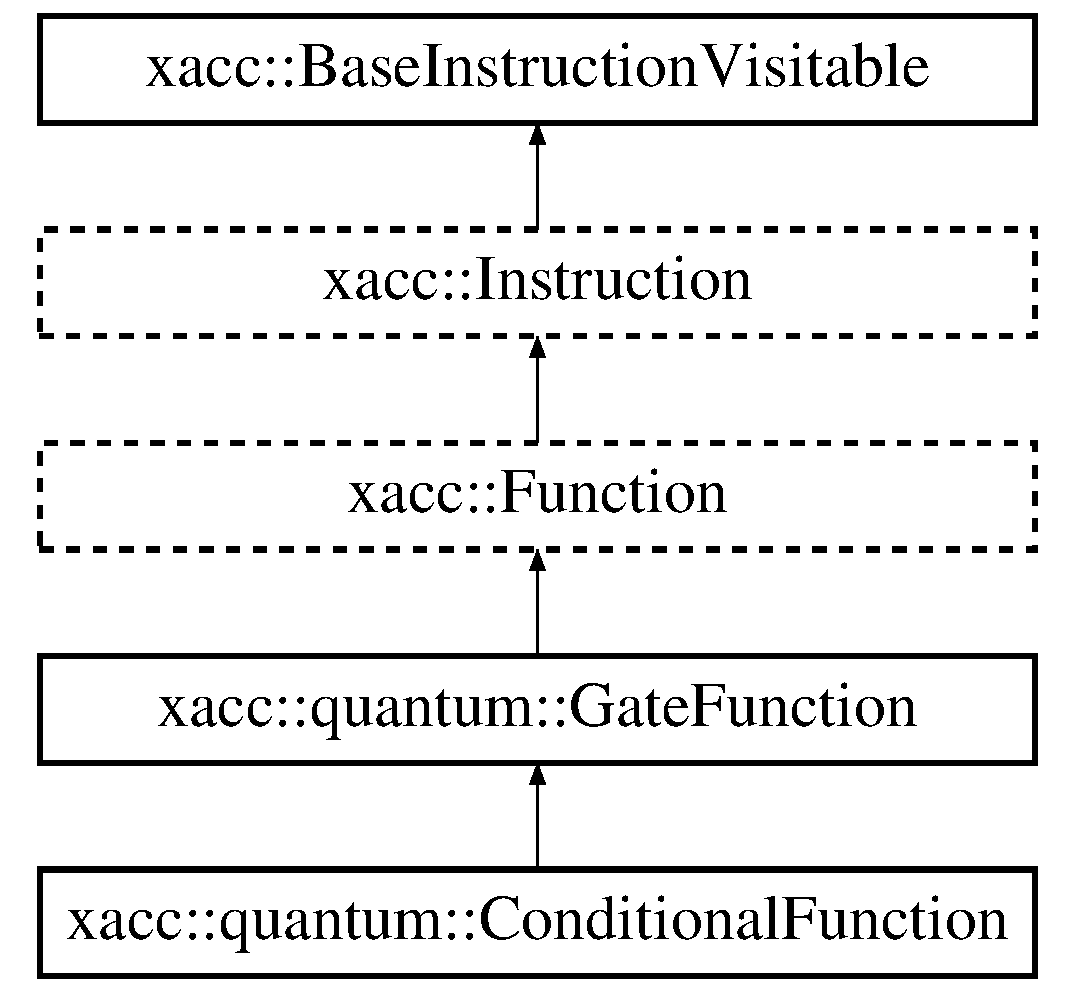
\includegraphics[height=5.000000cm]{a00040}
\end{center}
\end{figure}
\subsection*{Public Member Functions}
\begin{DoxyCompactItemize}
\item 
\hyperlink{a00040_a77545e72bd53268f609888654fcd8eee}{Gate\+Function} (const std\+::string \&name)
\item 
{\bfseries Gate\+Function} (const std\+::string \&name, std\+::vector$<$ Instruction\+Parameter $>$ params)\hypertarget{a00040_a0b1b3fb51a5b0f1bcb1b10692ab2e595}{}\label{a00040_a0b1b3fb51a5b0f1bcb1b10692ab2e595}

\item 
virtual const int \hyperlink{a00040_aa70b26156c060fec71316fe5e98bb102}{n\+Instructions} ()
\item 
virtual Inst\+Ptr \hyperlink{a00040_a841d656eed8aa9b4c0eec3f1da38069c}{get\+Instruction} (const int idx)
\item 
virtual std\+::list$<$ Inst\+Ptr $>$ \hyperlink{a00040_aebce6a9e64aed7f4aff86df752bacfe2}{get\+Instructions} ()
\item 
virtual void \hyperlink{a00040_a44ca35d081577de9ad2930f93c01e89d}{remove\+Instruction} (const int idx)
\item 
virtual void \hyperlink{a00040_a892fb69a10f0a7cb5abdab4cca61b80a}{add\+Instruction} (Inst\+Ptr instruction)
\item 
virtual void \hyperlink{a00040_a182fdfabbf546ae89e4f2384bafb45c9}{replace\+Instruction} (const int idx, Inst\+Ptr replacing\+Inst)
\item 
virtual void \hyperlink{a00040_aed3b963f1c4eb3215ca46af48d78f588}{insert\+Instruction} (const int idx, Inst\+Ptr new\+Inst)
\item 
virtual const std\+::string \hyperlink{a00040_af42efb6191267164717d53c469e15d3a}{get\+Name} ()
\item 
virtual const std\+::vector$<$ int $>$ \hyperlink{a00040_aba03de68b76a9e120705c3c389c714a1}{bits} ()
\item 
virtual const std\+::string \hyperlink{a00040_aa1950776ae84bad2d0795a0441f910e7}{to\+String} (const std\+::string \&buffer\+Var\+Name)
\item 
virtual Instruction\+Parameter \hyperlink{a00040_a5991903323e412777bedc4f0c862eb63}{get\+Parameter} (const int idx)
\item 
virtual void \hyperlink{a00040_ab8d9789b46e92e27a9d7c9c5b7e3683c}{set\+Parameter} (const int idx, Instruction\+Parameter \&p)
\item 
virtual std\+::vector$<$ Instruction\+Parameter $>$ \hyperlink{a00040_af7aabfe699a4dced576ff7fafff969d5}{get\+Parameters} ()
\item 
virtual bool \hyperlink{a00040_afad47903e0ed55ddbfa827ef8408a94b}{is\+Parameterized} ()
\item 
virtual const int \hyperlink{a00040_ad0bffcbc0884d81d6bdddf55385fc6c9}{n\+Parameters} ()
\item 
virtual void \hyperlink{a00040_a4bcbd2c8c4b615d74e4a4d39952fd411}{evaluate\+Variable\+Parameters} (std\+::vector$<$ Instruction\+Parameter $>$ runtime\+Parameters)
\end{DoxyCompactItemize}
\subsection*{Protected Attributes}
\begin{DoxyCompactItemize}
\item 
std\+::string \hyperlink{a00040_aea17cb1ca610bb5b8eadb0642c32b937}{function\+Name}
\item 
std\+::list$<$ Inst\+Ptr $>$ {\bfseries instructions}\hypertarget{a00040_aa2334b23541206ed02023ec28f5e4ac7}{}\label{a00040_aa2334b23541206ed02023ec28f5e4ac7}

\item 
std\+::vector$<$ Instruction\+Parameter $>$ {\bfseries parameters}\hypertarget{a00040_a2f53b483afa8d6b357f2550b8f1a3a9c}{}\label{a00040_a2f53b483afa8d6b357f2550b8f1a3a9c}

\item 
std\+::map$<$ int, std\+::pair$<$ int, std\+::string $>$ $>$ \hyperlink{a00040_a186fadb9c8b90481eaa260bdd81b37b9}{cached\+Variable\+Instructions}
\end{DoxyCompactItemize}
\subsection*{Additional Inherited Members}


\subsection{Detailed Description}
The \hyperlink{a00040}{Gate\+Function} is a Q\+Function for gate-\/model quantum computing. It is composed of Q\+Instructions that are themselves derivations of the \hyperlink{a00041}{Gate\+Instruction} class. 

\subsection{Constructor \& Destructor Documentation}
\index{xacc\+::quantum\+::\+Gate\+Function@{xacc\+::quantum\+::\+Gate\+Function}!Gate\+Function@{Gate\+Function}}
\index{Gate\+Function@{Gate\+Function}!xacc\+::quantum\+::\+Gate\+Function@{xacc\+::quantum\+::\+Gate\+Function}}
\subsubsection[{\texorpdfstring{Gate\+Function(const std\+::string \&name)}{GateFunction(const std::string \&name)}}]{\setlength{\rightskip}{0pt plus 5cm}xacc\+::quantum\+::\+Gate\+Function\+::\+Gate\+Function (
\begin{DoxyParamCaption}
\item[{const std\+::string \&}]{name}
\end{DoxyParamCaption}
)\hspace{0.3cm}{\ttfamily [inline]}}\hypertarget{a00040_a77545e72bd53268f609888654fcd8eee}{}\label{a00040_a77545e72bd53268f609888654fcd8eee}
The constructor, takes the function unique id and its name.


\begin{DoxyParams}{Parameters}
{\em id} & \\
\hline
{\em name} & \\
\hline
\end{DoxyParams}


\subsection{Member Function Documentation}
\index{xacc\+::quantum\+::\+Gate\+Function@{xacc\+::quantum\+::\+Gate\+Function}!add\+Instruction@{add\+Instruction}}
\index{add\+Instruction@{add\+Instruction}!xacc\+::quantum\+::\+Gate\+Function@{xacc\+::quantum\+::\+Gate\+Function}}
\subsubsection[{\texorpdfstring{add\+Instruction(\+Inst\+Ptr instruction)}{addInstruction(InstPtr instruction)}}]{\setlength{\rightskip}{0pt plus 5cm}virtual void xacc\+::quantum\+::\+Gate\+Function\+::add\+Instruction (
\begin{DoxyParamCaption}
\item[{Inst\+Ptr}]{instruction}
\end{DoxyParamCaption}
)\hspace{0.3cm}{\ttfamily [inline]}, {\ttfamily [virtual]}}\hypertarget{a00040_a892fb69a10f0a7cb5abdab4cca61b80a}{}\label{a00040_a892fb69a10f0a7cb5abdab4cca61b80a}
Add an instruction to this quantum intermediate representation.


\begin{DoxyParams}{Parameters}
{\em instruction} & \\
\hline
\end{DoxyParams}


Implements \hyperlink{a00038_aa8c9ec2d08be75c69399d4254b0216f5}{xacc\+::\+Function}.



Reimplemented in \hyperlink{a00025_a6aedad20f96390880efdc0a476b3273f}{xacc\+::quantum\+::\+Conditional\+Function}.

\index{xacc\+::quantum\+::\+Gate\+Function@{xacc\+::quantum\+::\+Gate\+Function}!bits@{bits}}
\index{bits@{bits}!xacc\+::quantum\+::\+Gate\+Function@{xacc\+::quantum\+::\+Gate\+Function}}
\subsubsection[{\texorpdfstring{bits()}{bits()}}]{\setlength{\rightskip}{0pt plus 5cm}virtual const std\+::vector$<$int$>$ xacc\+::quantum\+::\+Gate\+Function\+::bits (
\begin{DoxyParamCaption}
{}
\end{DoxyParamCaption}
)\hspace{0.3cm}{\ttfamily [inline]}, {\ttfamily [virtual]}}\hypertarget{a00040_aba03de68b76a9e120705c3c389c714a1}{}\label{a00040_aba03de68b76a9e120705c3c389c714a1}
Return the qubits this function acts on. \begin{DoxyReturn}{Returns}

\end{DoxyReturn}


Implements \hyperlink{a00046_a819f32e94c3e1c9e69a0061aaf8d86dc}{xacc\+::\+Instruction}.

\index{xacc\+::quantum\+::\+Gate\+Function@{xacc\+::quantum\+::\+Gate\+Function}!evaluate\+Variable\+Parameters@{evaluate\+Variable\+Parameters}}
\index{evaluate\+Variable\+Parameters@{evaluate\+Variable\+Parameters}!xacc\+::quantum\+::\+Gate\+Function@{xacc\+::quantum\+::\+Gate\+Function}}
\subsubsection[{\texorpdfstring{evaluate\+Variable\+Parameters(std\+::vector$<$ Instruction\+Parameter $>$ runtime\+Parameters)}{evaluateVariableParameters(std::vector< InstructionParameter > runtimeParameters)}}]{\setlength{\rightskip}{0pt plus 5cm}virtual void xacc\+::quantum\+::\+Gate\+Function\+::evaluate\+Variable\+Parameters (
\begin{DoxyParamCaption}
\item[{std\+::vector$<$ Instruction\+Parameter $>$}]{parameters}
\end{DoxyParamCaption}
)\hspace{0.3cm}{\ttfamily [inline]}, {\ttfamily [virtual]}}\hypertarget{a00040_a4bcbd2c8c4b615d74e4a4d39952fd411}{}\label{a00040_a4bcbd2c8c4b615d74e4a4d39952fd411}
This method is used to evaluate this \hyperlink{a00038}{Function}\textquotesingle{}s parameterized Instructions that have string variable Instruction\+Parameters. These parameters are updated with the given runtime parameters.


\begin{DoxyParams}{Parameters}
{\em parameters} & The runtime parameters \\
\hline
\end{DoxyParams}


Implements \hyperlink{a00038_af6ae9453027789a2aaec30e59c9e45e3}{xacc\+::\+Function}.

\index{xacc\+::quantum\+::\+Gate\+Function@{xacc\+::quantum\+::\+Gate\+Function}!get\+Instruction@{get\+Instruction}}
\index{get\+Instruction@{get\+Instruction}!xacc\+::quantum\+::\+Gate\+Function@{xacc\+::quantum\+::\+Gate\+Function}}
\subsubsection[{\texorpdfstring{get\+Instruction(const int idx)}{getInstruction(const int idx)}}]{\setlength{\rightskip}{0pt plus 5cm}virtual Inst\+Ptr xacc\+::quantum\+::\+Gate\+Function\+::get\+Instruction (
\begin{DoxyParamCaption}
\item[{const int}]{idx}
\end{DoxyParamCaption}
)\hspace{0.3cm}{\ttfamily [inline]}, {\ttfamily [virtual]}}\hypertarget{a00040_a841d656eed8aa9b4c0eec3f1da38069c}{}\label{a00040_a841d656eed8aa9b4c0eec3f1da38069c}
Return the \hyperlink{a00046}{Instruction} at the given index.


\begin{DoxyParams}{Parameters}
{\em idx} & The desired \hyperlink{a00046}{Instruction} index \\
\hline
\end{DoxyParams}
\begin{DoxyReturn}{Returns}
inst The instruction at the given index. 
\end{DoxyReturn}


Implements \hyperlink{a00038_afa549fc91b5a05f26d8139954a7e0ed5}{xacc\+::\+Function}.

\index{xacc\+::quantum\+::\+Gate\+Function@{xacc\+::quantum\+::\+Gate\+Function}!get\+Instructions@{get\+Instructions}}
\index{get\+Instructions@{get\+Instructions}!xacc\+::quantum\+::\+Gate\+Function@{xacc\+::quantum\+::\+Gate\+Function}}
\subsubsection[{\texorpdfstring{get\+Instructions()}{getInstructions()}}]{\setlength{\rightskip}{0pt plus 5cm}virtual std\+::list$<$Inst\+Ptr$>$ xacc\+::quantum\+::\+Gate\+Function\+::get\+Instructions (
\begin{DoxyParamCaption}
{}
\end{DoxyParamCaption}
)\hspace{0.3cm}{\ttfamily [inline]}, {\ttfamily [virtual]}}\hypertarget{a00040_aebce6a9e64aed7f4aff86df752bacfe2}{}\label{a00040_aebce6a9e64aed7f4aff86df752bacfe2}
Return all Instructions in this \hyperlink{a00038}{Function}

\begin{DoxyReturn}{Returns}
insts The list of this \hyperlink{a00038}{Function}\textquotesingle{}s Instructions 
\end{DoxyReturn}


Implements \hyperlink{a00038_aaf80bd3d49113a92b520785572663032}{xacc\+::\+Function}.

\index{xacc\+::quantum\+::\+Gate\+Function@{xacc\+::quantum\+::\+Gate\+Function}!get\+Name@{get\+Name}}
\index{get\+Name@{get\+Name}!xacc\+::quantum\+::\+Gate\+Function@{xacc\+::quantum\+::\+Gate\+Function}}
\subsubsection[{\texorpdfstring{get\+Name()}{getName()}}]{\setlength{\rightskip}{0pt plus 5cm}virtual const std\+::string xacc\+::quantum\+::\+Gate\+Function\+::get\+Name (
\begin{DoxyParamCaption}
{}
\end{DoxyParamCaption}
)\hspace{0.3cm}{\ttfamily [inline]}, {\ttfamily [virtual]}}\hypertarget{a00040_af42efb6191267164717d53c469e15d3a}{}\label{a00040_af42efb6191267164717d53c469e15d3a}
Return the name of this function \begin{DoxyReturn}{Returns}

\end{DoxyReturn}


Implements \hyperlink{a00046_ac7ff23f693e2276edbf3fdac5452792c}{xacc\+::\+Instruction}.

\index{xacc\+::quantum\+::\+Gate\+Function@{xacc\+::quantum\+::\+Gate\+Function}!get\+Parameter@{get\+Parameter}}
\index{get\+Parameter@{get\+Parameter}!xacc\+::quantum\+::\+Gate\+Function@{xacc\+::quantum\+::\+Gate\+Function}}
\subsubsection[{\texorpdfstring{get\+Parameter(const int idx)}{getParameter(const int idx)}}]{\setlength{\rightskip}{0pt plus 5cm}virtual Instruction\+Parameter xacc\+::quantum\+::\+Gate\+Function\+::get\+Parameter (
\begin{DoxyParamCaption}
\item[{const int}]{idx}
\end{DoxyParamCaption}
)\hspace{0.3cm}{\ttfamily [inline]}, {\ttfamily [virtual]}}\hypertarget{a00040_a5991903323e412777bedc4f0c862eb63}{}\label{a00040_a5991903323e412777bedc4f0c862eb63}
Return this \hyperlink{a00046}{Instruction}\textquotesingle{}s parameter at the given index.


\begin{DoxyParams}{Parameters}
{\em idx} & The index of the parameter. \\
\hline
\end{DoxyParams}
\begin{DoxyReturn}{Returns}
param The Instruction\+Parameter at the given index. 
\end{DoxyReturn}


Implements \hyperlink{a00046_aa0d9de97a4833a042379647f83c33ab6}{xacc\+::\+Instruction}.

\index{xacc\+::quantum\+::\+Gate\+Function@{xacc\+::quantum\+::\+Gate\+Function}!get\+Parameters@{get\+Parameters}}
\index{get\+Parameters@{get\+Parameters}!xacc\+::quantum\+::\+Gate\+Function@{xacc\+::quantum\+::\+Gate\+Function}}
\subsubsection[{\texorpdfstring{get\+Parameters()}{getParameters()}}]{\setlength{\rightskip}{0pt plus 5cm}virtual std\+::vector$<$Instruction\+Parameter$>$ xacc\+::quantum\+::\+Gate\+Function\+::get\+Parameters (
\begin{DoxyParamCaption}
{}
\end{DoxyParamCaption}
)\hspace{0.3cm}{\ttfamily [inline]}, {\ttfamily [virtual]}}\hypertarget{a00040_af7aabfe699a4dced576ff7fafff969d5}{}\label{a00040_af7aabfe699a4dced576ff7fafff969d5}
Return all of this \hyperlink{a00046}{Instruction}\textquotesingle{}s parameters.

\begin{DoxyReturn}{Returns}
params This instructions parameters. 
\end{DoxyReturn}


Implements \hyperlink{a00046_aeb67c67713896e8f27a5c7dd531f3340}{xacc\+::\+Instruction}.

\index{xacc\+::quantum\+::\+Gate\+Function@{xacc\+::quantum\+::\+Gate\+Function}!insert\+Instruction@{insert\+Instruction}}
\index{insert\+Instruction@{insert\+Instruction}!xacc\+::quantum\+::\+Gate\+Function@{xacc\+::quantum\+::\+Gate\+Function}}
\subsubsection[{\texorpdfstring{insert\+Instruction(const int idx, Inst\+Ptr new\+Inst)}{insertInstruction(const int idx, InstPtr newInst)}}]{\setlength{\rightskip}{0pt plus 5cm}virtual void xacc\+::quantum\+::\+Gate\+Function\+::insert\+Instruction (
\begin{DoxyParamCaption}
\item[{const int}]{idx, }
\item[{Inst\+Ptr}]{new\+Inst}
\end{DoxyParamCaption}
)\hspace{0.3cm}{\ttfamily [inline]}, {\ttfamily [virtual]}}\hypertarget{a00040_aed3b963f1c4eb3215ca46af48d78f588}{}\label{a00040_aed3b963f1c4eb3215ca46af48d78f588}
Insert a new \hyperlink{a00046}{Instruction} at the given index. All previous instructions are pushed back, ie their new indices are current\+Index + 1.


\begin{DoxyParams}{Parameters}
{\em idx} & The index where the new instruction should be inserted \\
\hline
{\em new\+Inst} & The new \hyperlink{a00046}{Instruction} to insert. \\
\hline
\end{DoxyParams}


Implements \hyperlink{a00038_acde702e44bdbc2759b338365218d7ebe}{xacc\+::\+Function}.

\index{xacc\+::quantum\+::\+Gate\+Function@{xacc\+::quantum\+::\+Gate\+Function}!is\+Parameterized@{is\+Parameterized}}
\index{is\+Parameterized@{is\+Parameterized}!xacc\+::quantum\+::\+Gate\+Function@{xacc\+::quantum\+::\+Gate\+Function}}
\subsubsection[{\texorpdfstring{is\+Parameterized()}{isParameterized()}}]{\setlength{\rightskip}{0pt plus 5cm}virtual bool xacc\+::quantum\+::\+Gate\+Function\+::is\+Parameterized (
\begin{DoxyParamCaption}
{}
\end{DoxyParamCaption}
)\hspace{0.3cm}{\ttfamily [inline]}, {\ttfamily [virtual]}}\hypertarget{a00040_afad47903e0ed55ddbfa827ef8408a94b}{}\label{a00040_afad47903e0ed55ddbfa827ef8408a94b}
Return true if this \hyperlink{a00046}{Instruction} is parameterized.

\begin{DoxyReturn}{Returns}
parameterized True if this \hyperlink{a00046}{Instruction} has parameters. 
\end{DoxyReturn}


Reimplemented from \hyperlink{a00046_a7b24d8ae485369fc2b2df7a3224a5e26}{xacc\+::\+Instruction}.

\index{xacc\+::quantum\+::\+Gate\+Function@{xacc\+::quantum\+::\+Gate\+Function}!n\+Instructions@{n\+Instructions}}
\index{n\+Instructions@{n\+Instructions}!xacc\+::quantum\+::\+Gate\+Function@{xacc\+::quantum\+::\+Gate\+Function}}
\subsubsection[{\texorpdfstring{n\+Instructions()}{nInstructions()}}]{\setlength{\rightskip}{0pt plus 5cm}virtual const int xacc\+::quantum\+::\+Gate\+Function\+::n\+Instructions (
\begin{DoxyParamCaption}
{}
\end{DoxyParamCaption}
)\hspace{0.3cm}{\ttfamily [inline]}, {\ttfamily [virtual]}}\hypertarget{a00040_aa70b26156c060fec71316fe5e98bb102}{}\label{a00040_aa70b26156c060fec71316fe5e98bb102}
Return the number of Instructions that this \hyperlink{a00038}{Function} contains.

\begin{DoxyReturn}{Returns}
n\+Inst The number of instructions 
\end{DoxyReturn}


Implements \hyperlink{a00038_a8901985525f59713e14c61713e07c086}{xacc\+::\+Function}.

\index{xacc\+::quantum\+::\+Gate\+Function@{xacc\+::quantum\+::\+Gate\+Function}!n\+Parameters@{n\+Parameters}}
\index{n\+Parameters@{n\+Parameters}!xacc\+::quantum\+::\+Gate\+Function@{xacc\+::quantum\+::\+Gate\+Function}}
\subsubsection[{\texorpdfstring{n\+Parameters()}{nParameters()}}]{\setlength{\rightskip}{0pt plus 5cm}virtual const int xacc\+::quantum\+::\+Gate\+Function\+::n\+Parameters (
\begin{DoxyParamCaption}
{}
\end{DoxyParamCaption}
)\hspace{0.3cm}{\ttfamily [inline]}, {\ttfamily [virtual]}}\hypertarget{a00040_ad0bffcbc0884d81d6bdddf55385fc6c9}{}\label{a00040_ad0bffcbc0884d81d6bdddf55385fc6c9}
Return the number of Instruction\+Parameters this \hyperlink{a00046}{Instruction} contains.

\begin{DoxyReturn}{Returns}
n\+Insts The number of instructions. 
\end{DoxyReturn}


Implements \hyperlink{a00046_ad54585d13c04ffd20296fff7ab8107ff}{xacc\+::\+Instruction}.

\index{xacc\+::quantum\+::\+Gate\+Function@{xacc\+::quantum\+::\+Gate\+Function}!remove\+Instruction@{remove\+Instruction}}
\index{remove\+Instruction@{remove\+Instruction}!xacc\+::quantum\+::\+Gate\+Function@{xacc\+::quantum\+::\+Gate\+Function}}
\subsubsection[{\texorpdfstring{remove\+Instruction(const int idx)}{removeInstruction(const int idx)}}]{\setlength{\rightskip}{0pt plus 5cm}virtual void xacc\+::quantum\+::\+Gate\+Function\+::remove\+Instruction (
\begin{DoxyParamCaption}
\item[{const int}]{idx}
\end{DoxyParamCaption}
)\hspace{0.3cm}{\ttfamily [inline]}, {\ttfamily [virtual]}}\hypertarget{a00040_a44ca35d081577de9ad2930f93c01e89d}{}\label{a00040_a44ca35d081577de9ad2930f93c01e89d}
Remove the \hyperlink{a00046}{Instruction} at the given index.


\begin{DoxyParams}{Parameters}
{\em idx} & The index of the \hyperlink{a00046}{Instruction} to remove. \\
\hline
\end{DoxyParams}


Implements \hyperlink{a00038_ab6478b09bb28e194bb555b3180737733}{xacc\+::\+Function}.

\index{xacc\+::quantum\+::\+Gate\+Function@{xacc\+::quantum\+::\+Gate\+Function}!replace\+Instruction@{replace\+Instruction}}
\index{replace\+Instruction@{replace\+Instruction}!xacc\+::quantum\+::\+Gate\+Function@{xacc\+::quantum\+::\+Gate\+Function}}
\subsubsection[{\texorpdfstring{replace\+Instruction(const int idx, Inst\+Ptr replacing\+Inst)}{replaceInstruction(const int idx, InstPtr replacingInst)}}]{\setlength{\rightskip}{0pt plus 5cm}virtual void xacc\+::quantum\+::\+Gate\+Function\+::replace\+Instruction (
\begin{DoxyParamCaption}
\item[{const int}]{idx, }
\item[{Inst\+Ptr}]{replacing\+Inst}
\end{DoxyParamCaption}
)\hspace{0.3cm}{\ttfamily [inline]}, {\ttfamily [virtual]}}\hypertarget{a00040_a182fdfabbf546ae89e4f2384bafb45c9}{}\label{a00040_a182fdfabbf546ae89e4f2384bafb45c9}
Replace the given current quantum instruction with the new replacing\+Inst quantum \hyperlink{a00046}{Instruction}.


\begin{DoxyParams}{Parameters}
{\em current\+Inst} & \\
\hline
{\em replacing\+Inst} & \\
\hline
\end{DoxyParams}


Implements \hyperlink{a00038_a2ef6a4923a6734f90f6ee3d94d263af0}{xacc\+::\+Function}.

\index{xacc\+::quantum\+::\+Gate\+Function@{xacc\+::quantum\+::\+Gate\+Function}!set\+Parameter@{set\+Parameter}}
\index{set\+Parameter@{set\+Parameter}!xacc\+::quantum\+::\+Gate\+Function@{xacc\+::quantum\+::\+Gate\+Function}}
\subsubsection[{\texorpdfstring{set\+Parameter(const int idx, Instruction\+Parameter \&p)}{setParameter(const int idx, InstructionParameter \&p)}}]{\setlength{\rightskip}{0pt plus 5cm}virtual void xacc\+::quantum\+::\+Gate\+Function\+::set\+Parameter (
\begin{DoxyParamCaption}
\item[{const int}]{idx, }
\item[{Instruction\+Parameter \&}]{isnt}
\end{DoxyParamCaption}
)\hspace{0.3cm}{\ttfamily [inline]}, {\ttfamily [virtual]}}\hypertarget{a00040_ab8d9789b46e92e27a9d7c9c5b7e3683c}{}\label{a00040_ab8d9789b46e92e27a9d7c9c5b7e3683c}
Set this \hyperlink{a00046}{Instruction}\textquotesingle{}s parameter at the given index.


\begin{DoxyParams}{Parameters}
{\em idx} & The index of the parameter \\
\hline
{\em inst} & The instruction. \\
\hline
\end{DoxyParams}


Implements \hyperlink{a00046_a407a0ac662fa0b1ec3e301e8ff9bade7}{xacc\+::\+Instruction}.

\index{xacc\+::quantum\+::\+Gate\+Function@{xacc\+::quantum\+::\+Gate\+Function}!to\+String@{to\+String}}
\index{to\+String@{to\+String}!xacc\+::quantum\+::\+Gate\+Function@{xacc\+::quantum\+::\+Gate\+Function}}
\subsubsection[{\texorpdfstring{to\+String(const std\+::string \&buffer\+Var\+Name)}{toString(const std::string \&bufferVarName)}}]{\setlength{\rightskip}{0pt plus 5cm}virtual const std\+::string xacc\+::quantum\+::\+Gate\+Function\+::to\+String (
\begin{DoxyParamCaption}
\item[{const std\+::string \&}]{buffer\+Var\+Name}
\end{DoxyParamCaption}
)\hspace{0.3cm}{\ttfamily [inline]}, {\ttfamily [virtual]}}\hypertarget{a00040_aa1950776ae84bad2d0795a0441f910e7}{}\label{a00040_aa1950776ae84bad2d0795a0441f910e7}
Return an assembly-\/like string representation for this function . 
\begin{DoxyParams}{Parameters}
{\em buffer\+Var\+Name} & \\
\hline
\end{DoxyParams}
\begin{DoxyReturn}{Returns}

\end{DoxyReturn}


Implements \hyperlink{a00046_ae94c2d089908294c1d410b14c96817ae}{xacc\+::\+Instruction}.



Reimplemented in \hyperlink{a00025_aca7a5f849fece6fc28a904efee9a3370}{xacc\+::quantum\+::\+Conditional\+Function}.



\subsection{Member Data Documentation}
\index{xacc\+::quantum\+::\+Gate\+Function@{xacc\+::quantum\+::\+Gate\+Function}!cached\+Variable\+Instructions@{cached\+Variable\+Instructions}}
\index{cached\+Variable\+Instructions@{cached\+Variable\+Instructions}!xacc\+::quantum\+::\+Gate\+Function@{xacc\+::quantum\+::\+Gate\+Function}}
\subsubsection[{\texorpdfstring{cached\+Variable\+Instructions}{cachedVariableInstructions}}]{\setlength{\rightskip}{0pt plus 5cm}std\+::map$<$int, std\+::pair$<$int, std\+::string$>$ $>$ xacc\+::quantum\+::\+Gate\+Function\+::cached\+Variable\+Instructions\hspace{0.3cm}{\ttfamily [protected]}}\hypertarget{a00040_a186fadb9c8b90481eaa260bdd81b37b9}{}\label{a00040_a186fadb9c8b90481eaa260bdd81b37b9}
Map of \hyperlink{a00046}{Instruction} Index to ( \hyperlink{a00046}{Instruction}\textquotesingle{}s Runtime Parameter Index, Dependent Variable name) \index{xacc\+::quantum\+::\+Gate\+Function@{xacc\+::quantum\+::\+Gate\+Function}!function\+Name@{function\+Name}}
\index{function\+Name@{function\+Name}!xacc\+::quantum\+::\+Gate\+Function@{xacc\+::quantum\+::\+Gate\+Function}}
\subsubsection[{\texorpdfstring{function\+Name}{functionName}}]{\setlength{\rightskip}{0pt plus 5cm}std\+::string xacc\+::quantum\+::\+Gate\+Function\+::function\+Name\hspace{0.3cm}{\ttfamily [protected]}}\hypertarget{a00040_aea17cb1ca610bb5b8eadb0642c32b937}{}\label{a00040_aea17cb1ca610bb5b8eadb0642c32b937}
The name of this function 

The documentation for this class was generated from the following file\+:\begin{DoxyCompactItemize}
\item 
Gate\+Function.\+hpp\end{DoxyCompactItemize}

\hypertarget{a00041}{}\section{xacc\+:\+:quantum\+:\+:Gate\+Instruction Class Reference}
\label{a00041}\index{xacc\+::quantum\+::\+Gate\+Instruction@{xacc\+::quantum\+::\+Gate\+Instruction}}
Inheritance diagram for xacc\+:\+:quantum\+:\+:Gate\+Instruction\+:\begin{figure}[H]
\begin{center}
\leavevmode
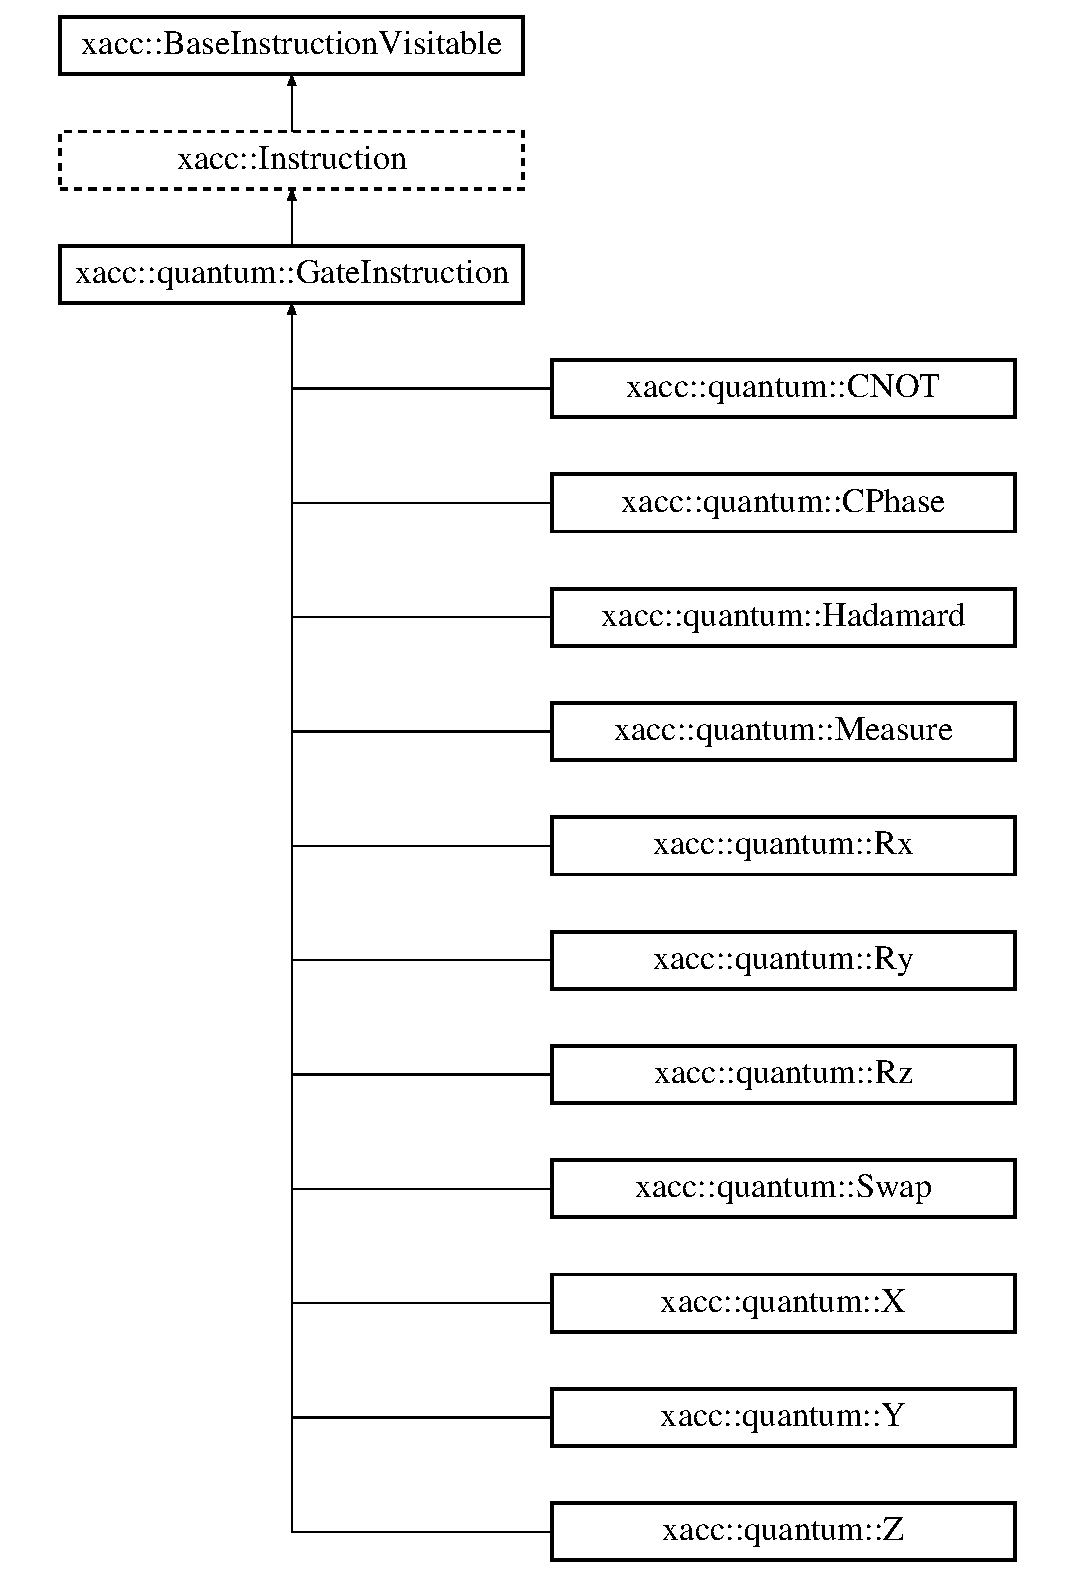
\includegraphics[height=12.000000cm]{a00041}
\end{center}
\end{figure}
\subsection*{Public Member Functions}
\begin{DoxyCompactItemize}
\item 
{\bfseries Gate\+Instruction} (std\+::vector$<$ int $>$ qubts)\hypertarget{a00041_a951ac3f44fcfbcf187bb73ba7438b472}{}\label{a00041_a951ac3f44fcfbcf187bb73ba7438b472}

\item 
\hyperlink{a00041_a9b8543b79576c69ab8578ab6228134d7}{Gate\+Instruction} (std\+::string name, std\+::vector$<$ int $>$ qubts)
\item 
{\bfseries Gate\+Instruction} (std\+::string name, std\+::vector$<$ int $>$ qubts, std\+::vector$<$ Instruction\+Parameter $>$ params)\hypertarget{a00041_a37aaeebdb14747b0afd7d00cf285343e}{}\label{a00041_a37aaeebdb14747b0afd7d00cf285343e}

\item 
virtual const std\+::string \hyperlink{a00041_a0db03b9e46eeba1134f0ca2b83ccc842}{get\+Name} ()
\item 
virtual const std\+::vector$<$ int $>$ \hyperlink{a00041_ad32ad03dfc516e00093030e60178003d}{bits} ()
\item 
virtual const std\+::string \hyperlink{a00041_a089a5da67ff40ac1a6f56e64589822d9}{to\+String} (const std\+::string \&buffer\+Var\+Name)
\item 
virtual bool \hyperlink{a00041_a0a821be322b0c848b01c55f91fc8f484}{is\+Enabled} ()
\item 
virtual void \hyperlink{a00041_a63ce138dd71fb43d303f5600fefb7215}{disable} ()
\item 
virtual void \hyperlink{a00041_a7a80474b7fd465271b3313432db2e608}{enable} ()
\item 
virtual Instruction\+Parameter \hyperlink{a00041_addd6185279fe99fbdc3d4efd96e42162}{get\+Parameter} (const int idx)
\item 
virtual void \hyperlink{a00041_afb8f7582d7520c77d61b9016753f5669}{set\+Parameter} (const int idx, Instruction\+Parameter \&p)
\item 
virtual std\+::vector$<$ Instruction\+Parameter $>$ \hyperlink{a00041_a8584444f9577283f6844ab32bdc4db72}{get\+Parameters} ()
\item 
virtual bool \hyperlink{a00041_afe7aeeb398262931e156bcb3950f8188}{is\+Parameterized} ()
\item 
virtual const int \hyperlink{a00041_a3752912b2c402668ca4814e21d4bbd26}{n\+Parameters} ()
\item 
virtual \hyperlink{a00041_ab8a75144074b27262fc33c77db4528b7}{$\sim$\+Gate\+Instruction} ()
\end{DoxyCompactItemize}
\subsection*{Protected Attributes}
\begin{DoxyCompactItemize}
\item 
std\+::string \hyperlink{a00041_a9961e6979139ced70300188cf2e4ad3f}{gate\+Name}
\item 
std\+::vector$<$ int $>$ \hyperlink{a00041_a2a56be6c2519ea65df4d06f4abae1393}{qbits}
\item 
bool {\bfseries enabled} = true\hypertarget{a00041_aa1039a127aa645a5c2206ef64e20b37a}{}\label{a00041_aa1039a127aa645a5c2206ef64e20b37a}

\item 
std\+::vector$<$ Instruction\+Parameter $>$ {\bfseries parameters}\hypertarget{a00041_a191e4c405f8413b7e8fc86fde07c0dd1}{}\label{a00041_a191e4c405f8413b7e8fc86fde07c0dd1}

\end{DoxyCompactItemize}
\subsection*{Additional Inherited Members}


\subsection{Constructor \& Destructor Documentation}
\index{xacc\+::quantum\+::\+Gate\+Instruction@{xacc\+::quantum\+::\+Gate\+Instruction}!Gate\+Instruction@{Gate\+Instruction}}
\index{Gate\+Instruction@{Gate\+Instruction}!xacc\+::quantum\+::\+Gate\+Instruction@{xacc\+::quantum\+::\+Gate\+Instruction}}
\subsubsection[{\texorpdfstring{Gate\+Instruction(std\+::string name, std\+::vector$<$ int $>$ qubts)}{GateInstruction(std::string name, std::vector< int > qubts)}}]{\setlength{\rightskip}{0pt plus 5cm}xacc\+::quantum\+::\+Gate\+Instruction\+::\+Gate\+Instruction (
\begin{DoxyParamCaption}
\item[{std\+::string}]{name, }
\item[{std\+::vector$<$ int $>$}]{qubts}
\end{DoxyParamCaption}
)\hspace{0.3cm}{\ttfamily [inline]}}\hypertarget{a00041_a9b8543b79576c69ab8578ab6228134d7}{}\label{a00041_a9b8543b79576c69ab8578ab6228134d7}
The constructor, takes the id, name, layer, and qubits this instruction acts on.


\begin{DoxyParams}{Parameters}
{\em id} & \\
\hline
{\em layer} & \\
\hline
{\em name} & \\
\hline
{\em qubts} & \\
\hline
\end{DoxyParams}
\index{xacc\+::quantum\+::\+Gate\+Instruction@{xacc\+::quantum\+::\+Gate\+Instruction}!````~Gate\+Instruction@{$\sim$\+Gate\+Instruction}}
\index{````~Gate\+Instruction@{$\sim$\+Gate\+Instruction}!xacc\+::quantum\+::\+Gate\+Instruction@{xacc\+::quantum\+::\+Gate\+Instruction}}
\subsubsection[{\texorpdfstring{$\sim$\+Gate\+Instruction()}{~GateInstruction()}}]{\setlength{\rightskip}{0pt plus 5cm}virtual xacc\+::quantum\+::\+Gate\+Instruction\+::$\sim$\+Gate\+Instruction (
\begin{DoxyParamCaption}
{}
\end{DoxyParamCaption}
)\hspace{0.3cm}{\ttfamily [inline]}, {\ttfamily [virtual]}}\hypertarget{a00041_ab8a75144074b27262fc33c77db4528b7}{}\label{a00041_ab8a75144074b27262fc33c77db4528b7}
The destructor 

\subsection{Member Function Documentation}
\index{xacc\+::quantum\+::\+Gate\+Instruction@{xacc\+::quantum\+::\+Gate\+Instruction}!bits@{bits}}
\index{bits@{bits}!xacc\+::quantum\+::\+Gate\+Instruction@{xacc\+::quantum\+::\+Gate\+Instruction}}
\subsubsection[{\texorpdfstring{bits()}{bits()}}]{\setlength{\rightskip}{0pt plus 5cm}virtual const std\+::vector$<$int$>$ xacc\+::quantum\+::\+Gate\+Instruction\+::bits (
\begin{DoxyParamCaption}
{}
\end{DoxyParamCaption}
)\hspace{0.3cm}{\ttfamily [inline]}, {\ttfamily [virtual]}}\hypertarget{a00041_ad32ad03dfc516e00093030e60178003d}{}\label{a00041_ad32ad03dfc516e00093030e60178003d}
Return the list of qubits this instruction acts on. \begin{DoxyReturn}{Returns}

\end{DoxyReturn}


Implements \hyperlink{a00046_a819f32e94c3e1c9e69a0061aaf8d86dc}{xacc\+::\+Instruction}.

\index{xacc\+::quantum\+::\+Gate\+Instruction@{xacc\+::quantum\+::\+Gate\+Instruction}!disable@{disable}}
\index{disable@{disable}!xacc\+::quantum\+::\+Gate\+Instruction@{xacc\+::quantum\+::\+Gate\+Instruction}}
\subsubsection[{\texorpdfstring{disable()}{disable()}}]{\setlength{\rightskip}{0pt plus 5cm}virtual void xacc\+::quantum\+::\+Gate\+Instruction\+::disable (
\begin{DoxyParamCaption}
{}
\end{DoxyParamCaption}
)\hspace{0.3cm}{\ttfamily [inline]}, {\ttfamily [virtual]}}\hypertarget{a00041_a63ce138dd71fb43d303f5600fefb7215}{}\label{a00041_a63ce138dd71fb43d303f5600fefb7215}
Disable this \hyperlink{a00046}{Instruction} 

Reimplemented from \hyperlink{a00046_a6e528da15e05a94cc1d7db268c483271}{xacc\+::\+Instruction}.

\index{xacc\+::quantum\+::\+Gate\+Instruction@{xacc\+::quantum\+::\+Gate\+Instruction}!enable@{enable}}
\index{enable@{enable}!xacc\+::quantum\+::\+Gate\+Instruction@{xacc\+::quantum\+::\+Gate\+Instruction}}
\subsubsection[{\texorpdfstring{enable()}{enable()}}]{\setlength{\rightskip}{0pt plus 5cm}virtual void xacc\+::quantum\+::\+Gate\+Instruction\+::enable (
\begin{DoxyParamCaption}
{}
\end{DoxyParamCaption}
)\hspace{0.3cm}{\ttfamily [inline]}, {\ttfamily [virtual]}}\hypertarget{a00041_a7a80474b7fd465271b3313432db2e608}{}\label{a00041_a7a80474b7fd465271b3313432db2e608}
Enable this \hyperlink{a00046}{Instruction}. 

Reimplemented from \hyperlink{a00046_a0b4f2e5a591af28342a3c08e4305e24f}{xacc\+::\+Instruction}.

\index{xacc\+::quantum\+::\+Gate\+Instruction@{xacc\+::quantum\+::\+Gate\+Instruction}!get\+Name@{get\+Name}}
\index{get\+Name@{get\+Name}!xacc\+::quantum\+::\+Gate\+Instruction@{xacc\+::quantum\+::\+Gate\+Instruction}}
\subsubsection[{\texorpdfstring{get\+Name()}{getName()}}]{\setlength{\rightskip}{0pt plus 5cm}virtual const std\+::string xacc\+::quantum\+::\+Gate\+Instruction\+::get\+Name (
\begin{DoxyParamCaption}
{}
\end{DoxyParamCaption}
)\hspace{0.3cm}{\ttfamily [inline]}, {\ttfamily [virtual]}}\hypertarget{a00041_a0db03b9e46eeba1134f0ca2b83ccc842}{}\label{a00041_a0db03b9e46eeba1134f0ca2b83ccc842}
Return the instruction name. \begin{DoxyReturn}{Returns}

\end{DoxyReturn}


Implements \hyperlink{a00046_ac7ff23f693e2276edbf3fdac5452792c}{xacc\+::\+Instruction}.

\index{xacc\+::quantum\+::\+Gate\+Instruction@{xacc\+::quantum\+::\+Gate\+Instruction}!get\+Parameter@{get\+Parameter}}
\index{get\+Parameter@{get\+Parameter}!xacc\+::quantum\+::\+Gate\+Instruction@{xacc\+::quantum\+::\+Gate\+Instruction}}
\subsubsection[{\texorpdfstring{get\+Parameter(const int idx)}{getParameter(const int idx)}}]{\setlength{\rightskip}{0pt plus 5cm}virtual Instruction\+Parameter xacc\+::quantum\+::\+Gate\+Instruction\+::get\+Parameter (
\begin{DoxyParamCaption}
\item[{const int}]{idx}
\end{DoxyParamCaption}
)\hspace{0.3cm}{\ttfamily [inline]}, {\ttfamily [virtual]}}\hypertarget{a00041_addd6185279fe99fbdc3d4efd96e42162}{}\label{a00041_addd6185279fe99fbdc3d4efd96e42162}
Return this \hyperlink{a00046}{Instruction}\textquotesingle{}s parameter at the given index.


\begin{DoxyParams}{Parameters}
{\em idx} & The index of the parameter. \\
\hline
\end{DoxyParams}
\begin{DoxyReturn}{Returns}
param The Instruction\+Parameter at the given index. 
\end{DoxyReturn}


Implements \hyperlink{a00046_aa0d9de97a4833a042379647f83c33ab6}{xacc\+::\+Instruction}.

\index{xacc\+::quantum\+::\+Gate\+Instruction@{xacc\+::quantum\+::\+Gate\+Instruction}!get\+Parameters@{get\+Parameters}}
\index{get\+Parameters@{get\+Parameters}!xacc\+::quantum\+::\+Gate\+Instruction@{xacc\+::quantum\+::\+Gate\+Instruction}}
\subsubsection[{\texorpdfstring{get\+Parameters()}{getParameters()}}]{\setlength{\rightskip}{0pt plus 5cm}virtual std\+::vector$<$Instruction\+Parameter$>$ xacc\+::quantum\+::\+Gate\+Instruction\+::get\+Parameters (
\begin{DoxyParamCaption}
{}
\end{DoxyParamCaption}
)\hspace{0.3cm}{\ttfamily [inline]}, {\ttfamily [virtual]}}\hypertarget{a00041_a8584444f9577283f6844ab32bdc4db72}{}\label{a00041_a8584444f9577283f6844ab32bdc4db72}
Return all of this \hyperlink{a00046}{Instruction}\textquotesingle{}s parameters.

\begin{DoxyReturn}{Returns}
params This instructions parameters. 
\end{DoxyReturn}


Implements \hyperlink{a00046_aeb67c67713896e8f27a5c7dd531f3340}{xacc\+::\+Instruction}.

\index{xacc\+::quantum\+::\+Gate\+Instruction@{xacc\+::quantum\+::\+Gate\+Instruction}!is\+Enabled@{is\+Enabled}}
\index{is\+Enabled@{is\+Enabled}!xacc\+::quantum\+::\+Gate\+Instruction@{xacc\+::quantum\+::\+Gate\+Instruction}}
\subsubsection[{\texorpdfstring{is\+Enabled()}{isEnabled()}}]{\setlength{\rightskip}{0pt plus 5cm}virtual bool xacc\+::quantum\+::\+Gate\+Instruction\+::is\+Enabled (
\begin{DoxyParamCaption}
{}
\end{DoxyParamCaption}
)\hspace{0.3cm}{\ttfamily [inline]}, {\ttfamily [virtual]}}\hypertarget{a00041_a0a821be322b0c848b01c55f91fc8f484}{}\label{a00041_a0a821be322b0c848b01c55f91fc8f484}
Returns true if this \hyperlink{a00046}{Instruction} is enabled

\begin{DoxyReturn}{Returns}
enabled True if this \hyperlink{a00046}{Instruction} is enabled. 
\end{DoxyReturn}


Reimplemented from \hyperlink{a00046_ad02a1cf7220577124720b7a51424cea7}{xacc\+::\+Instruction}.

\index{xacc\+::quantum\+::\+Gate\+Instruction@{xacc\+::quantum\+::\+Gate\+Instruction}!is\+Parameterized@{is\+Parameterized}}
\index{is\+Parameterized@{is\+Parameterized}!xacc\+::quantum\+::\+Gate\+Instruction@{xacc\+::quantum\+::\+Gate\+Instruction}}
\subsubsection[{\texorpdfstring{is\+Parameterized()}{isParameterized()}}]{\setlength{\rightskip}{0pt plus 5cm}virtual bool xacc\+::quantum\+::\+Gate\+Instruction\+::is\+Parameterized (
\begin{DoxyParamCaption}
{}
\end{DoxyParamCaption}
)\hspace{0.3cm}{\ttfamily [inline]}, {\ttfamily [virtual]}}\hypertarget{a00041_afe7aeeb398262931e156bcb3950f8188}{}\label{a00041_afe7aeeb398262931e156bcb3950f8188}
Return true if this \hyperlink{a00046}{Instruction} is parameterized.

\begin{DoxyReturn}{Returns}
parameterized True if this \hyperlink{a00046}{Instruction} has parameters. 
\end{DoxyReturn}


Reimplemented from \hyperlink{a00046_a7b24d8ae485369fc2b2df7a3224a5e26}{xacc\+::\+Instruction}.

\index{xacc\+::quantum\+::\+Gate\+Instruction@{xacc\+::quantum\+::\+Gate\+Instruction}!n\+Parameters@{n\+Parameters}}
\index{n\+Parameters@{n\+Parameters}!xacc\+::quantum\+::\+Gate\+Instruction@{xacc\+::quantum\+::\+Gate\+Instruction}}
\subsubsection[{\texorpdfstring{n\+Parameters()}{nParameters()}}]{\setlength{\rightskip}{0pt plus 5cm}virtual const int xacc\+::quantum\+::\+Gate\+Instruction\+::n\+Parameters (
\begin{DoxyParamCaption}
{}
\end{DoxyParamCaption}
)\hspace{0.3cm}{\ttfamily [inline]}, {\ttfamily [virtual]}}\hypertarget{a00041_a3752912b2c402668ca4814e21d4bbd26}{}\label{a00041_a3752912b2c402668ca4814e21d4bbd26}
Return the number of Instruction\+Parameters this \hyperlink{a00046}{Instruction} contains.

\begin{DoxyReturn}{Returns}
n\+Insts The number of instructions. 
\end{DoxyReturn}


Implements \hyperlink{a00046_ad54585d13c04ffd20296fff7ab8107ff}{xacc\+::\+Instruction}.

\index{xacc\+::quantum\+::\+Gate\+Instruction@{xacc\+::quantum\+::\+Gate\+Instruction}!set\+Parameter@{set\+Parameter}}
\index{set\+Parameter@{set\+Parameter}!xacc\+::quantum\+::\+Gate\+Instruction@{xacc\+::quantum\+::\+Gate\+Instruction}}
\subsubsection[{\texorpdfstring{set\+Parameter(const int idx, Instruction\+Parameter \&p)}{setParameter(const int idx, InstructionParameter \&p)}}]{\setlength{\rightskip}{0pt plus 5cm}virtual void xacc\+::quantum\+::\+Gate\+Instruction\+::set\+Parameter (
\begin{DoxyParamCaption}
\item[{const int}]{idx, }
\item[{Instruction\+Parameter \&}]{isnt}
\end{DoxyParamCaption}
)\hspace{0.3cm}{\ttfamily [inline]}, {\ttfamily [virtual]}}\hypertarget{a00041_afb8f7582d7520c77d61b9016753f5669}{}\label{a00041_afb8f7582d7520c77d61b9016753f5669}
Set this \hyperlink{a00046}{Instruction}\textquotesingle{}s parameter at the given index.


\begin{DoxyParams}{Parameters}
{\em idx} & The index of the parameter \\
\hline
{\em inst} & The instruction. \\
\hline
\end{DoxyParams}


Implements \hyperlink{a00046_a407a0ac662fa0b1ec3e301e8ff9bade7}{xacc\+::\+Instruction}.

\index{xacc\+::quantum\+::\+Gate\+Instruction@{xacc\+::quantum\+::\+Gate\+Instruction}!to\+String@{to\+String}}
\index{to\+String@{to\+String}!xacc\+::quantum\+::\+Gate\+Instruction@{xacc\+::quantum\+::\+Gate\+Instruction}}
\subsubsection[{\texorpdfstring{to\+String(const std\+::string \&buffer\+Var\+Name)}{toString(const std::string \&bufferVarName)}}]{\setlength{\rightskip}{0pt plus 5cm}virtual const std\+::string xacc\+::quantum\+::\+Gate\+Instruction\+::to\+String (
\begin{DoxyParamCaption}
\item[{const std\+::string \&}]{buffer\+Var\+Name}
\end{DoxyParamCaption}
)\hspace{0.3cm}{\ttfamily [inline]}, {\ttfamily [virtual]}}\hypertarget{a00041_a089a5da67ff40ac1a6f56e64589822d9}{}\label{a00041_a089a5da67ff40ac1a6f56e64589822d9}
Return this instruction\textquotesingle{}s assembly-\/like string representation. 
\begin{DoxyParams}{Parameters}
{\em buffer\+Var\+Name} & \\
\hline
\end{DoxyParams}
\begin{DoxyReturn}{Returns}

\end{DoxyReturn}


Implements \hyperlink{a00046_ae94c2d089908294c1d410b14c96817ae}{xacc\+::\+Instruction}.



Reimplemented in \hyperlink{a00055_a1c51a5d68294dcb2ba1a9fbea63a730f}{xacc\+::quantum\+::\+Measure}.



\subsection{Member Data Documentation}
\index{xacc\+::quantum\+::\+Gate\+Instruction@{xacc\+::quantum\+::\+Gate\+Instruction}!gate\+Name@{gate\+Name}}
\index{gate\+Name@{gate\+Name}!xacc\+::quantum\+::\+Gate\+Instruction@{xacc\+::quantum\+::\+Gate\+Instruction}}
\subsubsection[{\texorpdfstring{gate\+Name}{gateName}}]{\setlength{\rightskip}{0pt plus 5cm}std\+::string xacc\+::quantum\+::\+Gate\+Instruction\+::gate\+Name\hspace{0.3cm}{\ttfamily [protected]}}\hypertarget{a00041_a9961e6979139ced70300188cf2e4ad3f}{}\label{a00041_a9961e6979139ced70300188cf2e4ad3f}
Reference to this instructions name \index{xacc\+::quantum\+::\+Gate\+Instruction@{xacc\+::quantum\+::\+Gate\+Instruction}!qbits@{qbits}}
\index{qbits@{qbits}!xacc\+::quantum\+::\+Gate\+Instruction@{xacc\+::quantum\+::\+Gate\+Instruction}}
\subsubsection[{\texorpdfstring{qbits}{qbits}}]{\setlength{\rightskip}{0pt plus 5cm}std\+::vector$<$int$>$ xacc\+::quantum\+::\+Gate\+Instruction\+::qbits\hspace{0.3cm}{\ttfamily [protected]}}\hypertarget{a00041_a2a56be6c2519ea65df4d06f4abae1393}{}\label{a00041_a2a56be6c2519ea65df4d06f4abae1393}
Reference to the qubits this instruction acts on 

The documentation for this class was generated from the following file\+:\begin{DoxyCompactItemize}
\item 
Gate\+Instruction.\+hpp\end{DoxyCompactItemize}

\hypertarget{a00042}{}\section{xacc\+:\+:quantum\+:\+:Gate\+Q\+IR Class Reference}
\label{a00042}\index{xacc\+::quantum\+::\+Gate\+Q\+IR@{xacc\+::quantum\+::\+Gate\+Q\+IR}}


{\ttfamily \#include $<$Gate\+Q\+I\+R.\+hpp$>$}

Inheritance diagram for xacc\+:\+:quantum\+:\+:Gate\+Q\+IR\+:\begin{figure}[H]
\begin{center}
\leavevmode
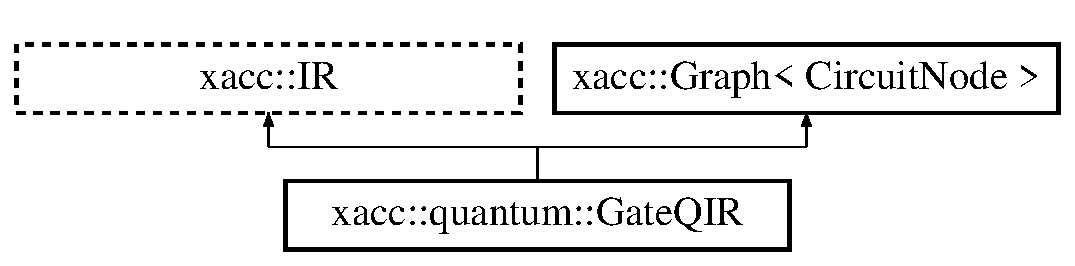
\includegraphics[height=2.000000cm]{a00042}
\end{center}
\end{figure}
\subsection*{Public Member Functions}
\begin{DoxyCompactItemize}
\item 
\hyperlink{a00042_afb99f610a6b123538c659169c131a634}{Gate\+Q\+IR} ()
\item 
virtual void \hyperlink{a00042_ad1ddd6105346dd9fc78648fd812285ed}{generate\+Graph} (const std\+::string \&kernel\+Name)
\item 
virtual void \hyperlink{a00042_aa6ed2cf2cbcfec8105c327a4fa95346f}{add\+Kernel} (std\+::shared\+\_\+ptr$<$ \hyperlink{a00038}{Function} $>$ kernel)
\item 
virtual const int {\bfseries number\+Of\+Kernels} ()\hypertarget{a00042_aca6be85526b14f500e7f98954dd6da5c}{}\label{a00042_aca6be85526b14f500e7f98954dd6da5c}

\item 
virtual std\+::shared\+\_\+ptr$<$ \hyperlink{a00038}{Function} $>$ \hyperlink{a00042_a194758b6edcc3ae0c7fe8004f9bfe690}{get\+Kernel} (const std\+::string \&name)
\item 
virtual bool \hyperlink{a00042_a692f95099caa7c024110a3f035941dca}{kernel\+Exists} (const std\+::string \&name)
\item 
virtual std\+::string \hyperlink{a00042_a7153f7e9f516d43af3d5d4f95d60bd86}{to\+Assembly\+String} (const std\+::string \&kernel\+Name, const std\+::string \&acc\+Buffer\+Var\+Name)
\item 
virtual void \hyperlink{a00042_a40e1d07e4dfd3794ef53fca3cdbdca61}{persist} (std\+::ostream \&out\+Stream)
\item 
virtual void \hyperlink{a00042_a07f26eeb362ac480d20da6cdc8c8fb39}{load} (std\+::istream \&in\+Stream)
\item 
virtual void \hyperlink{a00042_a26019e2f1e13e64645e29aee86ac58b1}{read} (std\+::istream \&stream)
\item 
virtual std\+::vector$<$ std\+::shared\+\_\+ptr$<$ \hyperlink{a00038}{Function} $>$ $>$ \hyperlink{a00042_a4ace7ee5ebef84b1f39aaf5ed12c6cc6}{get\+Kernels} ()
\item 
virtual \hyperlink{a00042_ac88db03f1dd29e2d36aaa6c01a130008}{$\sim$\+Gate\+Q\+IR} ()
\end{DoxyCompactItemize}
\subsection*{Protected Attributes}
\begin{DoxyCompactItemize}
\item 
std\+::vector$<$ std\+::shared\+\_\+ptr$<$ \hyperlink{a00038}{Function} $>$ $>$ \hyperlink{a00042_ae75a4af0ce455eee1ce316c16426a661}{kernels}
\end{DoxyCompactItemize}


\subsection{Detailed Description}
The \hyperlink{a00042}{Gate\+Q\+IR} is an implementation of the Q\+IR for gate model quantum computing. It provides a \hyperlink{a00043}{Graph} node type that models a quantum circuit gate (\hyperlink{a00020}{Circuit\+Node}). 

\subsection{Constructor \& Destructor Documentation}
\index{xacc\+::quantum\+::\+Gate\+Q\+IR@{xacc\+::quantum\+::\+Gate\+Q\+IR}!Gate\+Q\+IR@{Gate\+Q\+IR}}
\index{Gate\+Q\+IR@{Gate\+Q\+IR}!xacc\+::quantum\+::\+Gate\+Q\+IR@{xacc\+::quantum\+::\+Gate\+Q\+IR}}
\subsubsection[{\texorpdfstring{Gate\+Q\+I\+R()}{GateQIR()}}]{\setlength{\rightskip}{0pt plus 5cm}xacc\+::quantum\+::\+Gate\+Q\+I\+R\+::\+Gate\+Q\+IR (
\begin{DoxyParamCaption}
{}
\end{DoxyParamCaption}
)\hspace{0.3cm}{\ttfamily [inline]}}\hypertarget{a00042_afb99f610a6b123538c659169c131a634}{}\label{a00042_afb99f610a6b123538c659169c131a634}
The nullary Constructor \index{xacc\+::quantum\+::\+Gate\+Q\+IR@{xacc\+::quantum\+::\+Gate\+Q\+IR}!````~Gate\+Q\+IR@{$\sim$\+Gate\+Q\+IR}}
\index{````~Gate\+Q\+IR@{$\sim$\+Gate\+Q\+IR}!xacc\+::quantum\+::\+Gate\+Q\+IR@{xacc\+::quantum\+::\+Gate\+Q\+IR}}
\subsubsection[{\texorpdfstring{$\sim$\+Gate\+Q\+I\+R()}{~GateQIR()}}]{\setlength{\rightskip}{0pt plus 5cm}virtual xacc\+::quantum\+::\+Gate\+Q\+I\+R\+::$\sim$\+Gate\+Q\+IR (
\begin{DoxyParamCaption}
{}
\end{DoxyParamCaption}
)\hspace{0.3cm}{\ttfamily [inline]}, {\ttfamily [virtual]}}\hypertarget{a00042_ac88db03f1dd29e2d36aaa6c01a130008}{}\label{a00042_ac88db03f1dd29e2d36aaa6c01a130008}
The destructor 

\subsection{Member Function Documentation}
\index{xacc\+::quantum\+::\+Gate\+Q\+IR@{xacc\+::quantum\+::\+Gate\+Q\+IR}!add\+Kernel@{add\+Kernel}}
\index{add\+Kernel@{add\+Kernel}!xacc\+::quantum\+::\+Gate\+Q\+IR@{xacc\+::quantum\+::\+Gate\+Q\+IR}}
\subsubsection[{\texorpdfstring{add\+Kernel(std\+::shared\+\_\+ptr$<$ Function $>$ kernel)}{addKernel(std::shared\_ptr< Function > kernel)}}]{\setlength{\rightskip}{0pt plus 5cm}virtual void xacc\+::quantum\+::\+Gate\+Q\+I\+R\+::add\+Kernel (
\begin{DoxyParamCaption}
\item[{std\+::shared\+\_\+ptr$<$ {\bf Function} $>$}]{kernel}
\end{DoxyParamCaption}
)\hspace{0.3cm}{\ttfamily [inline]}, {\ttfamily [virtual]}}\hypertarget{a00042_aa6ed2cf2cbcfec8105c327a4fa95346f}{}\label{a00042_aa6ed2cf2cbcfec8105c327a4fa95346f}
Add a quantum function to this intermediate representation. 
\begin{DoxyParams}{Parameters}
{\em kernel} & \\
\hline
\end{DoxyParams}


Implements \hyperlink{a00050_abbbf8e6993c518597de32cd05d49d737}{xacc\+::\+IR}.

\index{xacc\+::quantum\+::\+Gate\+Q\+IR@{xacc\+::quantum\+::\+Gate\+Q\+IR}!generate\+Graph@{generate\+Graph}}
\index{generate\+Graph@{generate\+Graph}!xacc\+::quantum\+::\+Gate\+Q\+IR@{xacc\+::quantum\+::\+Gate\+Q\+IR}}
\subsubsection[{\texorpdfstring{generate\+Graph(const std\+::string \&kernel\+Name)}{generateGraph(const std::string \&kernelName)}}]{\setlength{\rightskip}{0pt plus 5cm}void xacc\+::quantum\+::\+Gate\+Q\+I\+R\+::generate\+Graph (
\begin{DoxyParamCaption}
\item[{const std\+::string \&}]{kernel\+Name}
\end{DoxyParamCaption}
)\hspace{0.3cm}{\ttfamily [virtual]}}\hypertarget{a00042_ad1ddd6105346dd9fc78648fd812285ed}{}\label{a00042_ad1ddd6105346dd9fc78648fd812285ed}
This method takes the list of quantum instructions that this Q\+IR contains and creates a graph representation of the quantum circuit. \index{xacc\+::quantum\+::\+Gate\+Q\+IR@{xacc\+::quantum\+::\+Gate\+Q\+IR}!get\+Kernel@{get\+Kernel}}
\index{get\+Kernel@{get\+Kernel}!xacc\+::quantum\+::\+Gate\+Q\+IR@{xacc\+::quantum\+::\+Gate\+Q\+IR}}
\subsubsection[{\texorpdfstring{get\+Kernel(const std\+::string \&name)}{getKernel(const std::string \&name)}}]{\setlength{\rightskip}{0pt plus 5cm}virtual std\+::shared\+\_\+ptr$<${\bf Function}$>$ xacc\+::quantum\+::\+Gate\+Q\+I\+R\+::get\+Kernel (
\begin{DoxyParamCaption}
\item[{const std\+::string \&}]{name}
\end{DoxyParamCaption}
)\hspace{0.3cm}{\ttfamily [inline]}, {\ttfamily [virtual]}}\hypertarget{a00042_a194758b6edcc3ae0c7fe8004f9bfe690}{}\label{a00042_a194758b6edcc3ae0c7fe8004f9bfe690}
Return the kernel with the given name.


\begin{DoxyParams}{Parameters}
{\em name} & The name of the kernel to return. \\
\hline
\end{DoxyParams}
\begin{DoxyReturn}{Returns}
kernel The kernel with given name. 
\end{DoxyReturn}


Implements \hyperlink{a00050_a6f49b4ba4b3a15142b04873284885f0d}{xacc\+::\+IR}.

\index{xacc\+::quantum\+::\+Gate\+Q\+IR@{xacc\+::quantum\+::\+Gate\+Q\+IR}!get\+Kernels@{get\+Kernels}}
\index{get\+Kernels@{get\+Kernels}!xacc\+::quantum\+::\+Gate\+Q\+IR@{xacc\+::quantum\+::\+Gate\+Q\+IR}}
\subsubsection[{\texorpdfstring{get\+Kernels()}{getKernels()}}]{\setlength{\rightskip}{0pt plus 5cm}virtual std\+::vector$<$std\+::shared\+\_\+ptr$<${\bf Function}$>$ $>$ xacc\+::quantum\+::\+Gate\+Q\+I\+R\+::get\+Kernels (
\begin{DoxyParamCaption}
{}
\end{DoxyParamCaption}
)\hspace{0.3cm}{\ttfamily [inline]}, {\ttfamily [virtual]}}\hypertarget{a00042_a4ace7ee5ebef84b1f39aaf5ed12c6cc6}{}\label{a00042_a4ace7ee5ebef84b1f39aaf5ed12c6cc6}
Return all of this \hyperlink{a00050}{IR} instance\textquotesingle{}s kernels.

\begin{DoxyReturn}{Returns}
kernels The kernels this \hyperlink{a00050}{IR} contains. 
\end{DoxyReturn}


Implements \hyperlink{a00050_a88c50bfc5b279145360ddc0c3a703b9b}{xacc\+::\+IR}.

\index{xacc\+::quantum\+::\+Gate\+Q\+IR@{xacc\+::quantum\+::\+Gate\+Q\+IR}!kernel\+Exists@{kernel\+Exists}}
\index{kernel\+Exists@{kernel\+Exists}!xacc\+::quantum\+::\+Gate\+Q\+IR@{xacc\+::quantum\+::\+Gate\+Q\+IR}}
\subsubsection[{\texorpdfstring{kernel\+Exists(const std\+::string \&name)}{kernelExists(const std::string \&name)}}]{\setlength{\rightskip}{0pt plus 5cm}virtual bool xacc\+::quantum\+::\+Gate\+Q\+I\+R\+::kernel\+Exists (
\begin{DoxyParamCaption}
\item[{const std\+::string \&}]{name}
\end{DoxyParamCaption}
)\hspace{0.3cm}{\ttfamily [inline]}, {\ttfamily [virtual]}}\hypertarget{a00042_a692f95099caa7c024110a3f035941dca}{}\label{a00042_a692f95099caa7c024110a3f035941dca}
Return true if the kernel with given name exists in this \hyperlink{a00050}{IR}.


\begin{DoxyParams}{Parameters}
{\em name} & The name of the kernel to return. \\
\hline
\end{DoxyParams}
\begin{DoxyReturn}{Returns}
exists True if kernel exists. 
\end{DoxyReturn}


Implements \hyperlink{a00050_afc9ccf5126f3fed19c2e879133b2f6d8}{xacc\+::\+IR}.

\index{xacc\+::quantum\+::\+Gate\+Q\+IR@{xacc\+::quantum\+::\+Gate\+Q\+IR}!load@{load}}
\index{load@{load}!xacc\+::quantum\+::\+Gate\+Q\+IR@{xacc\+::quantum\+::\+Gate\+Q\+IR}}
\subsubsection[{\texorpdfstring{load(std\+::istream \&in\+Stream)}{load(std::istream \&inStream)}}]{\setlength{\rightskip}{0pt plus 5cm}void xacc\+::quantum\+::\+Gate\+Q\+I\+R\+::load (
\begin{DoxyParamCaption}
\item[{std\+::istream \&}]{in\+Stream}
\end{DoxyParamCaption}
)\hspace{0.3cm}{\ttfamily [virtual]}}\hypertarget{a00042_a07f26eeb362ac480d20da6cdc8c8fb39}{}\label{a00042_a07f26eeb362ac480d20da6cdc8c8fb39}
Create this \hyperlink{a00050}{IR} instance from the given input stream.


\begin{DoxyParams}{Parameters}
{\em in\+Stream} & \\
\hline
\end{DoxyParams}


Implements \hyperlink{a00050_a444c2e4dc0faac500fb70fa93997e9bc}{xacc\+::\+IR}.

\index{xacc\+::quantum\+::\+Gate\+Q\+IR@{xacc\+::quantum\+::\+Gate\+Q\+IR}!persist@{persist}}
\index{persist@{persist}!xacc\+::quantum\+::\+Gate\+Q\+IR@{xacc\+::quantum\+::\+Gate\+Q\+IR}}
\subsubsection[{\texorpdfstring{persist(std\+::ostream \&out\+Stream)}{persist(std::ostream \&outStream)}}]{\setlength{\rightskip}{0pt plus 5cm}void xacc\+::quantum\+::\+Gate\+Q\+I\+R\+::persist (
\begin{DoxyParamCaption}
\item[{std\+::ostream \&}]{out\+Stream}
\end{DoxyParamCaption}
)\hspace{0.3cm}{\ttfamily [virtual]}}\hypertarget{a00042_a40e1d07e4dfd3794ef53fca3cdbdca61}{}\label{a00042_a40e1d07e4dfd3794ef53fca3cdbdca61}
Persist this \hyperlink{a00050}{IR} instance to the given output stream.


\begin{DoxyParams}{Parameters}
{\em out\+Stream} & \\
\hline
\end{DoxyParams}


Implements \hyperlink{a00050_a414b72224d88473ad6190bb88102a3ea}{xacc\+::\+IR}.

\index{xacc\+::quantum\+::\+Gate\+Q\+IR@{xacc\+::quantum\+::\+Gate\+Q\+IR}!read@{read}}
\index{read@{read}!xacc\+::quantum\+::\+Gate\+Q\+IR@{xacc\+::quantum\+::\+Gate\+Q\+IR}}
\subsubsection[{\texorpdfstring{read(std\+::istream \&stream)}{read(std::istream \&stream)}}]{\setlength{\rightskip}{0pt plus 5cm}void xacc\+::quantum\+::\+Gate\+Q\+I\+R\+::read (
\begin{DoxyParamCaption}
\item[{std\+::istream \&}]{stream}
\end{DoxyParamCaption}
)\hspace{0.3cm}{\ttfamily [virtual]}}\hypertarget{a00042_a26019e2f1e13e64645e29aee86ac58b1}{}\label{a00042_a26019e2f1e13e64645e29aee86ac58b1}
This is the implementation of the \hyperlink{a00043_abdd3e67dc08c223821d809bc8914164a}{Graph.\+read} method...

Read in a graphviz dot graph from the given input stream. This is left for subclasses.


\begin{DoxyParams}{Parameters}
{\em stream} & \\
\hline
\end{DoxyParams}


Reimplemented from \hyperlink{a00043_abdd3e67dc08c223821d809bc8914164a}{xacc\+::\+Graph$<$ Circuit\+Node $>$}.

\index{xacc\+::quantum\+::\+Gate\+Q\+IR@{xacc\+::quantum\+::\+Gate\+Q\+IR}!to\+Assembly\+String@{to\+Assembly\+String}}
\index{to\+Assembly\+String@{to\+Assembly\+String}!xacc\+::quantum\+::\+Gate\+Q\+IR@{xacc\+::quantum\+::\+Gate\+Q\+IR}}
\subsubsection[{\texorpdfstring{to\+Assembly\+String(const std\+::string \&kernel\+Name, const std\+::string \&acc\+Buffer\+Var\+Name)}{toAssemblyString(const std::string \&kernelName, const std::string \&accBufferVarName)}}]{\setlength{\rightskip}{0pt plus 5cm}std\+::string xacc\+::quantum\+::\+Gate\+Q\+I\+R\+::to\+Assembly\+String (
\begin{DoxyParamCaption}
\item[{const std\+::string \&}]{kernel\+Name, }
\item[{const std\+::string \&}]{acc\+Buffer\+Var\+Name}
\end{DoxyParamCaption}
)\hspace{0.3cm}{\ttfamily [virtual]}}\hypertarget{a00042_a7153f7e9f516d43af3d5d4f95d60bd86}{}\label{a00042_a7153f7e9f516d43af3d5d4f95d60bd86}
Return a string representation of this intermediate representation \begin{DoxyReturn}{Returns}

\end{DoxyReturn}


Implements \hyperlink{a00050_a8356cdff1919b88eabeb84fd7450cdb6}{xacc\+::\+IR}.



\subsection{Member Data Documentation}
\index{xacc\+::quantum\+::\+Gate\+Q\+IR@{xacc\+::quantum\+::\+Gate\+Q\+IR}!kernels@{kernels}}
\index{kernels@{kernels}!xacc\+::quantum\+::\+Gate\+Q\+IR@{xacc\+::quantum\+::\+Gate\+Q\+IR}}
\subsubsection[{\texorpdfstring{kernels}{kernels}}]{\setlength{\rightskip}{0pt plus 5cm}std\+::vector$<$std\+::shared\+\_\+ptr$<${\bf Function}$>$ $>$ xacc\+::quantum\+::\+Gate\+Q\+I\+R\+::kernels\hspace{0.3cm}{\ttfamily [protected]}}\hypertarget{a00042_ae75a4af0ce455eee1ce316c16426a661}{}\label{a00042_ae75a4af0ce455eee1ce316c16426a661}
Reference to this Q\+IR\textquotesingle{}s list of quantum functions 

The documentation for this class was generated from the following files\+:\begin{DoxyCompactItemize}
\item 
Gate\+Q\+I\+R.\+hpp\item 
Gate\+Q\+I\+R.\+cpp\end{DoxyCompactItemize}

\hypertarget{a00043}{}\section{xacc\+:\+:Graph$<$ Vertex, type $>$ Class Template Reference}
\label{a00043}\index{xacc\+::\+Graph$<$ Vertex, type $>$@{xacc\+::\+Graph$<$ Vertex, type $>$}}


{\ttfamily \#include $<$Graph.\+hpp$>$}

\subsection*{Classes}
\begin{DoxyCompactItemize}
\item 
class \hyperlink{a00086}{X\+A\+C\+C\+Vertex\+Properties\+Writer}
\end{DoxyCompactItemize}
\subsection*{Public Member Functions}
\begin{DoxyCompactItemize}
\item 
\hyperlink{a00043_a168a916da7346d0af307a75121f80ca4}{Graph} ()
\item 
\hyperlink{a00043_ab513bb56f7a3ede4891aafc586a31717}{Graph} (const int number\+Of\+Vertices)
\item 
void \hyperlink{a00043_a69ddb8cdc899ba47174f0e65b60a75dd}{add\+Edge} (const int src\+Index, const int tgt\+Index, const double edge\+Weight)
\item 
void \hyperlink{a00043_ae9dcc413d7e9b774b6bf2963c261f5fa}{add\+Edge} (const int src\+Index, const int tgt\+Index)
\item 
void {\bfseries remove\+Edge} (const int src\+Index, const int tgt\+Index)\hypertarget{a00043_ab146ca29c8c4edc8c36c2328927663ec}{}\label{a00043_ab146ca29c8c4edc8c36c2328927663ec}

\item 
void \hyperlink{a00043_a99f45a817a10a62dd5f2f8c9a1734d8a}{add\+Vertex} ()
\item 
{\footnotesize template$<$typename... Properties$>$ }\\void \hyperlink{a00043_aa96658ad91d64e71cbd7a88d479bf7e4}{add\+Vertex} (Properties...\+properties)
\item 
void {\bfseries add\+Vertex} (Vertex \&vertex)\hypertarget{a00043_a2eef95bbacd0a7194dea4f81beb1cb37}{}\label{a00043_a2eef95bbacd0a7194dea4f81beb1cb37}

\item 
{\footnotesize template$<$typename... Properties$>$ }\\void \hyperlink{a00043_abe79a4cb96d48abcd03df01dae73fcc3}{set\+Vertex\+Properties} (const int index, Properties...\+properties)
\item 
{\footnotesize template$<$const int Property\+Index$>$ }\\void \hyperlink{a00043_aeeb65835e8a16ebba34da08ea8016fac}{set\+Vertex\+Property} (const int index, decltype(std\+::get$<$ Property\+Index $>$(std\+::declval$<$ Vertex $>$().properties)) prop)
\item 
Vertex \& {\bfseries get\+Vertex} (const int index)\hypertarget{a00043_a401589d879abd25f69e38fd197138531}{}\label{a00043_a401589d879abd25f69e38fd197138531}

\item 
auto {\bfseries get\+Vertex\+Properties} (const int index) -\/$>$ decltype(($\ast$\+\_\+graph.\+get())\mbox{[}index\mbox{]}.properties)\hypertarget{a00043_abe1f333b2c9a9f597fb68c00bf44e7f7}{}\label{a00043_abe1f333b2c9a9f597fb68c00bf44e7f7}

\item 
{\footnotesize template$<$const int Property\+Index$>$ }\\decltype(std\+::get$<$ Property\+Index $>$(std\+::declval$<$ Vertex $>$().properties))\& \hyperlink{a00043_a394f58c21a234393f08b4c3a565a5940}{get\+Vertex\+Property} (const int index)
\item 
void \hyperlink{a00043_aaf1edd0f038f6cca1c3c9ece35d3ec05}{set\+Edge\+Weight} (const int src\+Index, const int tgt\+Index, const double weight)
\item 
double \hyperlink{a00043_a917e439598a91ace852ad67bba029f5c}{get\+Edge\+Weight} (const int src\+Index, const int tgt\+Index)
\item 
bool \hyperlink{a00043_acb5a6e586e58dbef53d84631134a1cdf}{edge\+Exists} (const int src\+Index, const int tgt\+Index)
\item 
int \hyperlink{a00043_afd0f6cc800e0d81f8c168d47c927cf02}{degree} (const int index)
\item 
int \hyperlink{a00043_a9da48591a9d5ec658ae8c62204821ea7}{diameter} ()
\item 
int \hyperlink{a00043_ae3138d390f1d1c7d335144b59df2ddac}{size} ()
\item 
int \hyperlink{a00043_a50fca47e555122b5bb72e93e719484b4}{order} ()
\item 
std\+::list$<$ int $>$ {\bfseries get\+Neighbor\+List} (const int index)\hypertarget{a00043_a0e2ea9abc71a4f5d0b6d2f796a64a23b}{}\label{a00043_a0e2ea9abc71a4f5d0b6d2f796a64a23b}

\item 
void \hyperlink{a00043_a56dbba0529135ffdebb4ac3fbdb69252}{write} (std\+::ostream \&stream)
\item 
virtual void \hyperlink{a00043_abdd3e67dc08c223821d809bc8914164a}{read} (std\+::istream \&stream)
\end{DoxyCompactItemize}
\subsection*{Protected Attributes}
\begin{DoxyCompactItemize}
\item 
Boost\+Graph \hyperlink{a00043_acc3a072e3a30cdb8107b571170d96694}{\+\_\+graph}
\end{DoxyCompactItemize}


\subsection{Detailed Description}
\subsubsection*{template$<$typename Vertex, Graph\+Type type = Undirected$>$\\*
class xacc\+::\+Graph$<$ Vertex, type $>$}

The \hyperlink{a00043}{Graph} class provides a generic data structure modeling mathematical graph structures. It is templated on the vertex type, allowing for graphs with a wide variety of graph nodes (for example, in quantum computing -\/ graph of tensors, graph of Ising parameters, etc.)

All provided Vertex types must be a subclass of the Q\+C\+I\+Vertex in order to properly provide a tuple of vertex properties. s 

\subsection{Constructor \& Destructor Documentation}
\index{xacc\+::\+Graph@{xacc\+::\+Graph}!Graph@{Graph}}
\index{Graph@{Graph}!xacc\+::\+Graph@{xacc\+::\+Graph}}
\subsubsection[{\texorpdfstring{Graph()}{Graph()}}]{\setlength{\rightskip}{0pt plus 5cm}template$<$typename Vertex, Graph\+Type type = Undirected$>$ {\bf xacc\+::\+Graph}$<$ Vertex, type $>$\+::{\bf Graph} (
\begin{DoxyParamCaption}
{}
\end{DoxyParamCaption}
)\hspace{0.3cm}{\ttfamily [inline]}}\hypertarget{a00043_a168a916da7346d0af307a75121f80ca4}{}\label{a00043_a168a916da7346d0af307a75121f80ca4}
The nullary constructor \index{xacc\+::\+Graph@{xacc\+::\+Graph}!Graph@{Graph}}
\index{Graph@{Graph}!xacc\+::\+Graph@{xacc\+::\+Graph}}
\subsubsection[{\texorpdfstring{Graph(const int number\+Of\+Vertices)}{Graph(const int numberOfVertices)}}]{\setlength{\rightskip}{0pt plus 5cm}template$<$typename Vertex, Graph\+Type type = Undirected$>$ {\bf xacc\+::\+Graph}$<$ Vertex, type $>$\+::{\bf Graph} (
\begin{DoxyParamCaption}
\item[{const int}]{number\+Of\+Vertices}
\end{DoxyParamCaption}
)\hspace{0.3cm}{\ttfamily [inline]}}\hypertarget{a00043_ab513bb56f7a3ede4891aafc586a31717}{}\label{a00043_ab513bb56f7a3ede4891aafc586a31717}
The constructor, constructs a graph with specified number of vertices.


\begin{DoxyParams}{Parameters}
{\em number\+Of\+Vertices} & The number of vertices \\
\hline
\end{DoxyParams}


\subsection{Member Function Documentation}
\index{xacc\+::\+Graph@{xacc\+::\+Graph}!add\+Edge@{add\+Edge}}
\index{add\+Edge@{add\+Edge}!xacc\+::\+Graph@{xacc\+::\+Graph}}
\subsubsection[{\texorpdfstring{add\+Edge(const int src\+Index, const int tgt\+Index, const double edge\+Weight)}{addEdge(const int srcIndex, const int tgtIndex, const double edgeWeight)}}]{\setlength{\rightskip}{0pt plus 5cm}template$<$typename Vertex, Graph\+Type type = Undirected$>$ void {\bf xacc\+::\+Graph}$<$ Vertex, type $>$\+::add\+Edge (
\begin{DoxyParamCaption}
\item[{const int}]{src\+Index, }
\item[{const int}]{tgt\+Index, }
\item[{const double}]{edge\+Weight}
\end{DoxyParamCaption}
)\hspace{0.3cm}{\ttfamily [inline]}}\hypertarget{a00043_a69ddb8cdc899ba47174f0e65b60a75dd}{}\label{a00043_a69ddb8cdc899ba47174f0e65b60a75dd}
Add an edge between the vertices with given provided indices and edge weight.


\begin{DoxyParams}{Parameters}
{\em src\+Index} & Index of the starting vertex \\
\hline
{\em tgt\+Index} & Index of the ending vertex \\
\hline
{\em edge\+Weight} & The edge weight \\
\hline
\end{DoxyParams}
\index{xacc\+::\+Graph@{xacc\+::\+Graph}!add\+Edge@{add\+Edge}}
\index{add\+Edge@{add\+Edge}!xacc\+::\+Graph@{xacc\+::\+Graph}}
\subsubsection[{\texorpdfstring{add\+Edge(const int src\+Index, const int tgt\+Index)}{addEdge(const int srcIndex, const int tgtIndex)}}]{\setlength{\rightskip}{0pt plus 5cm}template$<$typename Vertex, Graph\+Type type = Undirected$>$ void {\bf xacc\+::\+Graph}$<$ Vertex, type $>$\+::add\+Edge (
\begin{DoxyParamCaption}
\item[{const int}]{src\+Index, }
\item[{const int}]{tgt\+Index}
\end{DoxyParamCaption}
)\hspace{0.3cm}{\ttfamily [inline]}}\hypertarget{a00043_ae9dcc413d7e9b774b6bf2963c261f5fa}{}\label{a00043_ae9dcc413d7e9b774b6bf2963c261f5fa}
Add an edge with default edge weight between the vertices at the provided indices.


\begin{DoxyParams}{Parameters}
{\em src\+Index} & Index of the starting vertex \\
\hline
{\em tgt\+Index} & Index of the ending vertex \\
\hline
\end{DoxyParams}
\index{xacc\+::\+Graph@{xacc\+::\+Graph}!add\+Vertex@{add\+Vertex}}
\index{add\+Vertex@{add\+Vertex}!xacc\+::\+Graph@{xacc\+::\+Graph}}
\subsubsection[{\texorpdfstring{add\+Vertex()}{addVertex()}}]{\setlength{\rightskip}{0pt plus 5cm}template$<$typename Vertex, Graph\+Type type = Undirected$>$ void {\bf xacc\+::\+Graph}$<$ Vertex, type $>$\+::add\+Vertex (
\begin{DoxyParamCaption}
{}
\end{DoxyParamCaption}
)\hspace{0.3cm}{\ttfamily [inline]}}\hypertarget{a00043_a99f45a817a10a62dd5f2f8c9a1734d8a}{}\label{a00043_a99f45a817a10a62dd5f2f8c9a1734d8a}
Add a vertex to this \hyperlink{a00043}{Graph}. \index{xacc\+::\+Graph@{xacc\+::\+Graph}!add\+Vertex@{add\+Vertex}}
\index{add\+Vertex@{add\+Vertex}!xacc\+::\+Graph@{xacc\+::\+Graph}}
\subsubsection[{\texorpdfstring{add\+Vertex(\+Properties...\+properties)}{addVertex(Properties...properties)}}]{\setlength{\rightskip}{0pt plus 5cm}template$<$typename Vertex, Graph\+Type type = Undirected$>$ template$<$typename... Properties$>$ void {\bf xacc\+::\+Graph}$<$ Vertex, type $>$\+::add\+Vertex (
\begin{DoxyParamCaption}
\item[{Properties...}]{properties}
\end{DoxyParamCaption}
)\hspace{0.3cm}{\ttfamily [inline]}}\hypertarget{a00043_aa96658ad91d64e71cbd7a88d479bf7e4}{}\label{a00043_aa96658ad91d64e71cbd7a88d479bf7e4}
Add a vertex to this graph with the provided properties. s 
\begin{DoxyParams}{Parameters}
{\em properties} & \\
\hline
\end{DoxyParams}
\index{xacc\+::\+Graph@{xacc\+::\+Graph}!degree@{degree}}
\index{degree@{degree}!xacc\+::\+Graph@{xacc\+::\+Graph}}
\subsubsection[{\texorpdfstring{degree(const int index)}{degree(const int index)}}]{\setlength{\rightskip}{0pt plus 5cm}template$<$typename Vertex, Graph\+Type type = Undirected$>$ int {\bf xacc\+::\+Graph}$<$ Vertex, type $>$\+::degree (
\begin{DoxyParamCaption}
\item[{const int}]{index}
\end{DoxyParamCaption}
)\hspace{0.3cm}{\ttfamily [inline]}}\hypertarget{a00043_afd0f6cc800e0d81f8c168d47c927cf02}{}\label{a00043_afd0f6cc800e0d81f8c168d47c927cf02}
Return the vertex degree at the given vertex index.


\begin{DoxyParams}{Parameters}
{\em index} & The index of the vertex \\
\hline
\end{DoxyParams}
\begin{DoxyReturn}{Returns}
degree The degree of the vertex 
\end{DoxyReturn}
\index{xacc\+::\+Graph@{xacc\+::\+Graph}!diameter@{diameter}}
\index{diameter@{diameter}!xacc\+::\+Graph@{xacc\+::\+Graph}}
\subsubsection[{\texorpdfstring{diameter()}{diameter()}}]{\setlength{\rightskip}{0pt plus 5cm}template$<$typename Vertex, Graph\+Type type = Undirected$>$ int {\bf xacc\+::\+Graph}$<$ Vertex, type $>$\+::diameter (
\begin{DoxyParamCaption}
{}
\end{DoxyParamCaption}
)\hspace{0.3cm}{\ttfamily [inline]}}\hypertarget{a00043_a9da48591a9d5ec658ae8c62204821ea7}{}\label{a00043_a9da48591a9d5ec658ae8c62204821ea7}
Return the diameter of this \hyperlink{a00043}{Graph}.

\begin{DoxyReturn}{Returns}
diameter The graph diameter 
\end{DoxyReturn}
\index{xacc\+::\+Graph@{xacc\+::\+Graph}!edge\+Exists@{edge\+Exists}}
\index{edge\+Exists@{edge\+Exists}!xacc\+::\+Graph@{xacc\+::\+Graph}}
\subsubsection[{\texorpdfstring{edge\+Exists(const int src\+Index, const int tgt\+Index)}{edgeExists(const int srcIndex, const int tgtIndex)}}]{\setlength{\rightskip}{0pt plus 5cm}template$<$typename Vertex, Graph\+Type type = Undirected$>$ bool {\bf xacc\+::\+Graph}$<$ Vertex, type $>$\+::edge\+Exists (
\begin{DoxyParamCaption}
\item[{const int}]{src\+Index, }
\item[{const int}]{tgt\+Index}
\end{DoxyParamCaption}
)\hspace{0.3cm}{\ttfamily [inline]}}\hypertarget{a00043_acb5a6e586e58dbef53d84631134a1cdf}{}\label{a00043_acb5a6e586e58dbef53d84631134a1cdf}
Return true if there is an edge between the two vertices at the given vertex indices.


\begin{DoxyParams}{Parameters}
{\em src\+Index} & The starting vertex index \\
\hline
{\em tgt\+Index} & The ending vertex index \\
\hline
\end{DoxyParams}
\begin{DoxyReturn}{Returns}
exists Boolean indicating if edge exists or not 
\end{DoxyReturn}
\index{xacc\+::\+Graph@{xacc\+::\+Graph}!get\+Edge\+Weight@{get\+Edge\+Weight}}
\index{get\+Edge\+Weight@{get\+Edge\+Weight}!xacc\+::\+Graph@{xacc\+::\+Graph}}
\subsubsection[{\texorpdfstring{get\+Edge\+Weight(const int src\+Index, const int tgt\+Index)}{getEdgeWeight(const int srcIndex, const int tgtIndex)}}]{\setlength{\rightskip}{0pt plus 5cm}template$<$typename Vertex, Graph\+Type type = Undirected$>$ double {\bf xacc\+::\+Graph}$<$ Vertex, type $>$\+::get\+Edge\+Weight (
\begin{DoxyParamCaption}
\item[{const int}]{src\+Index, }
\item[{const int}]{tgt\+Index}
\end{DoxyParamCaption}
)\hspace{0.3cm}{\ttfamily [inline]}}\hypertarget{a00043_a917e439598a91ace852ad67bba029f5c}{}\label{a00043_a917e439598a91ace852ad67bba029f5c}
Return the edge weight at the edge between the provided vertices.


\begin{DoxyParams}{Parameters}
{\em src\+Index} & The starting vertex index \\
\hline
{\em tgt\+Index} & The ending vertex index \\
\hline
\end{DoxyParams}
\begin{DoxyReturn}{Returns}
The edge weight 
\end{DoxyReturn}
\index{xacc\+::\+Graph@{xacc\+::\+Graph}!get\+Vertex\+Property@{get\+Vertex\+Property}}
\index{get\+Vertex\+Property@{get\+Vertex\+Property}!xacc\+::\+Graph@{xacc\+::\+Graph}}
\subsubsection[{\texorpdfstring{get\+Vertex\+Property(const int index)}{getVertexProperty(const int index)}}]{\setlength{\rightskip}{0pt plus 5cm}template$<$typename Vertex, Graph\+Type type = Undirected$>$ template$<$const int Property\+Index$>$ decltype(std\+::get$<$Property\+Index$>$(std\+::declval$<$Vertex$>$().properties)) \& {\bf xacc\+::\+Graph}$<$ Vertex, type $>$\+::get\+Vertex\+Property (
\begin{DoxyParamCaption}
\item[{const int}]{index}
\end{DoxyParamCaption}
)\hspace{0.3cm}{\ttfamily [inline]}}\hypertarget{a00043_a394f58c21a234393f08b4c3a565a5940}{}\label{a00043_a394f58c21a234393f08b4c3a565a5940}
Return the vertex property of the vertex at the given index and at the provided valid vertex property template index.


\begin{DoxyParams}{Parameters}
{\em index} & The index of the vertex \\
\hline
\end{DoxyParams}
\begin{DoxyReturn}{Returns}
property The property value. 
\end{DoxyReturn}
\index{xacc\+::\+Graph@{xacc\+::\+Graph}!order@{order}}
\index{order@{order}!xacc\+::\+Graph@{xacc\+::\+Graph}}
\subsubsection[{\texorpdfstring{order()}{order()}}]{\setlength{\rightskip}{0pt plus 5cm}template$<$typename Vertex, Graph\+Type type = Undirected$>$ int {\bf xacc\+::\+Graph}$<$ Vertex, type $>$\+::order (
\begin{DoxyParamCaption}
{}
\end{DoxyParamCaption}
)\hspace{0.3cm}{\ttfamily [inline]}}\hypertarget{a00043_a50fca47e555122b5bb72e93e719484b4}{}\label{a00043_a50fca47e555122b5bb72e93e719484b4}
Return the number of vertices in this graph

\begin{DoxyReturn}{Returns}
n\+Verts The number of vertices. 
\end{DoxyReturn}
\index{xacc\+::\+Graph@{xacc\+::\+Graph}!read@{read}}
\index{read@{read}!xacc\+::\+Graph@{xacc\+::\+Graph}}
\subsubsection[{\texorpdfstring{read(std\+::istream \&stream)}{read(std::istream \&stream)}}]{\setlength{\rightskip}{0pt plus 5cm}template$<$typename Vertex, Graph\+Type type = Undirected$>$ virtual void {\bf xacc\+::\+Graph}$<$ Vertex, type $>$\+::read (
\begin{DoxyParamCaption}
\item[{std\+::istream \&}]{stream}
\end{DoxyParamCaption}
)\hspace{0.3cm}{\ttfamily [inline]}, {\ttfamily [virtual]}}\hypertarget{a00043_abdd3e67dc08c223821d809bc8914164a}{}\label{a00043_abdd3e67dc08c223821d809bc8914164a}
Read in a graphviz dot graph from the given input stream. This is left for subclasses.


\begin{DoxyParams}{Parameters}
{\em stream} & \\
\hline
\end{DoxyParams}


Reimplemented in \hyperlink{a00042_a26019e2f1e13e64645e29aee86ac58b1}{xacc\+::quantum\+::\+Gate\+Q\+IR}, and \hyperlink{a00061_af7a7f4a487d493fe8a4ed1f76cefd731}{xacc\+::quantum\+::\+Quantum\+Circuit}.

\index{xacc\+::\+Graph@{xacc\+::\+Graph}!set\+Edge\+Weight@{set\+Edge\+Weight}}
\index{set\+Edge\+Weight@{set\+Edge\+Weight}!xacc\+::\+Graph@{xacc\+::\+Graph}}
\subsubsection[{\texorpdfstring{set\+Edge\+Weight(const int src\+Index, const int tgt\+Index, const double weight)}{setEdgeWeight(const int srcIndex, const int tgtIndex, const double weight)}}]{\setlength{\rightskip}{0pt plus 5cm}template$<$typename Vertex, Graph\+Type type = Undirected$>$ void {\bf xacc\+::\+Graph}$<$ Vertex, type $>$\+::set\+Edge\+Weight (
\begin{DoxyParamCaption}
\item[{const int}]{src\+Index, }
\item[{const int}]{tgt\+Index, }
\item[{const double}]{weight}
\end{DoxyParamCaption}
)\hspace{0.3cm}{\ttfamily [inline]}}\hypertarget{a00043_aaf1edd0f038f6cca1c3c9ece35d3ec05}{}\label{a00043_aaf1edd0f038f6cca1c3c9ece35d3ec05}
Set the weight on the edge between the vertices at the provided indices.


\begin{DoxyParams}{Parameters}
{\em src\+Index} & The starting vertex index \\
\hline
{\em tgt\+Index} & The ending vertex index \\
\hline
{\em weight} & The weight to set. \\
\hline
\end{DoxyParams}
\index{xacc\+::\+Graph@{xacc\+::\+Graph}!set\+Vertex\+Properties@{set\+Vertex\+Properties}}
\index{set\+Vertex\+Properties@{set\+Vertex\+Properties}!xacc\+::\+Graph@{xacc\+::\+Graph}}
\subsubsection[{\texorpdfstring{set\+Vertex\+Properties(const int index, Properties...\+properties)}{setVertexProperties(const int index, Properties...properties)}}]{\setlength{\rightskip}{0pt plus 5cm}template$<$typename Vertex, Graph\+Type type = Undirected$>$ template$<$typename... Properties$>$ void {\bf xacc\+::\+Graph}$<$ Vertex, type $>$\+::set\+Vertex\+Properties (
\begin{DoxyParamCaption}
\item[{const int}]{index, }
\item[{Properties...}]{properties}
\end{DoxyParamCaption}
)\hspace{0.3cm}{\ttfamily [inline]}}\hypertarget{a00043_abe79a4cb96d48abcd03df01dae73fcc3}{}\label{a00043_abe79a4cb96d48abcd03df01dae73fcc3}
Set an existing vertices properties.


\begin{DoxyParams}{Parameters}
{\em index} & The index of the vertex \\
\hline
{\em properties} & The new properties for the vertex \\
\hline
\end{DoxyParams}
\index{xacc\+::\+Graph@{xacc\+::\+Graph}!set\+Vertex\+Property@{set\+Vertex\+Property}}
\index{set\+Vertex\+Property@{set\+Vertex\+Property}!xacc\+::\+Graph@{xacc\+::\+Graph}}
\subsubsection[{\texorpdfstring{set\+Vertex\+Property(const int index, decltype(std\+::get$<$ Property\+Index $>$(std\+::declval$<$ Vertex $>$().\+properties)) prop)}{setVertexProperty(const int index, decltype(std::get< PropertyIndex >(std::declval< Vertex >().properties)) prop)}}]{\setlength{\rightskip}{0pt plus 5cm}template$<$typename Vertex, Graph\+Type type = Undirected$>$ template$<$const int Property\+Index$>$ void {\bf xacc\+::\+Graph}$<$ Vertex, type $>$\+::set\+Vertex\+Property (
\begin{DoxyParamCaption}
\item[{const int}]{index, }
\item[{decltype(std\+::get$<$ Property\+Index $>$(std\+::declval$<$ Vertex $>$().properties))}]{prop}
\end{DoxyParamCaption}
)\hspace{0.3cm}{\ttfamily [inline]}}\hypertarget{a00043_aeeb65835e8a16ebba34da08ea8016fac}{}\label{a00043_aeeb65835e8a16ebba34da08ea8016fac}
Set a specific vertex property for the vertex at given index.


\begin{DoxyParams}{Parameters}
{\em index} & The index of the vertex \\
\hline
{\em prop} & The property to set. \\
\hline
\end{DoxyParams}
\index{xacc\+::\+Graph@{xacc\+::\+Graph}!size@{size}}
\index{size@{size}!xacc\+::\+Graph@{xacc\+::\+Graph}}
\subsubsection[{\texorpdfstring{size()}{size()}}]{\setlength{\rightskip}{0pt plus 5cm}template$<$typename Vertex, Graph\+Type type = Undirected$>$ int {\bf xacc\+::\+Graph}$<$ Vertex, type $>$\+::size (
\begin{DoxyParamCaption}
{}
\end{DoxyParamCaption}
)\hspace{0.3cm}{\ttfamily [inline]}}\hypertarget{a00043_ae3138d390f1d1c7d335144b59df2ddac}{}\label{a00043_ae3138d390f1d1c7d335144b59df2ddac}
Return the number of edges. \begin{DoxyReturn}{Returns}
n\+Edges The number of edges. 
\end{DoxyReturn}
\index{xacc\+::\+Graph@{xacc\+::\+Graph}!write@{write}}
\index{write@{write}!xacc\+::\+Graph@{xacc\+::\+Graph}}
\subsubsection[{\texorpdfstring{write(std\+::ostream \&stream)}{write(std::ostream \&stream)}}]{\setlength{\rightskip}{0pt plus 5cm}template$<$typename Vertex, Graph\+Type type = Undirected$>$ void {\bf xacc\+::\+Graph}$<$ Vertex, type $>$\+::write (
\begin{DoxyParamCaption}
\item[{std\+::ostream \&}]{stream}
\end{DoxyParamCaption}
)\hspace{0.3cm}{\ttfamily [inline]}}\hypertarget{a00043_a56dbba0529135ffdebb4ac3fbdb69252}{}\label{a00043_a56dbba0529135ffdebb4ac3fbdb69252}
Write this graph in a graphviz dot format to the provided ostream.


\begin{DoxyParams}{Parameters}
{\em stream} & \\
\hline
\end{DoxyParams}


\subsection{Member Data Documentation}
\index{xacc\+::\+Graph@{xacc\+::\+Graph}!\+\_\+graph@{\+\_\+graph}}
\index{\+\_\+graph@{\+\_\+graph}!xacc\+::\+Graph@{xacc\+::\+Graph}}
\subsubsection[{\texorpdfstring{\+\_\+graph}{\_graph}}]{\setlength{\rightskip}{0pt plus 5cm}template$<$typename Vertex, Graph\+Type type = Undirected$>$ Boost\+Graph {\bf xacc\+::\+Graph}$<$ Vertex, type $>$\+::\+\_\+graph\hspace{0.3cm}{\ttfamily [protected]}}\hypertarget{a00043_acc3a072e3a30cdb8107b571170d96694}{}\label{a00043_acc3a072e3a30cdb8107b571170d96694}
The actual graph data structure we are delegating to. 

The documentation for this class was generated from the following file\+:\begin{DoxyCompactItemize}
\item 
Graph.\+hpp\end{DoxyCompactItemize}

\hypertarget{a00044}{}\section{xacc\+:\+:quantum\+:\+:Hadamard Class Reference}
\label{a00044}\index{xacc\+::quantum\+::\+Hadamard@{xacc\+::quantum\+::\+Hadamard}}
Inheritance diagram for xacc\+:\+:quantum\+:\+:Hadamard\+:\begin{figure}[H]
\begin{center}
\leavevmode
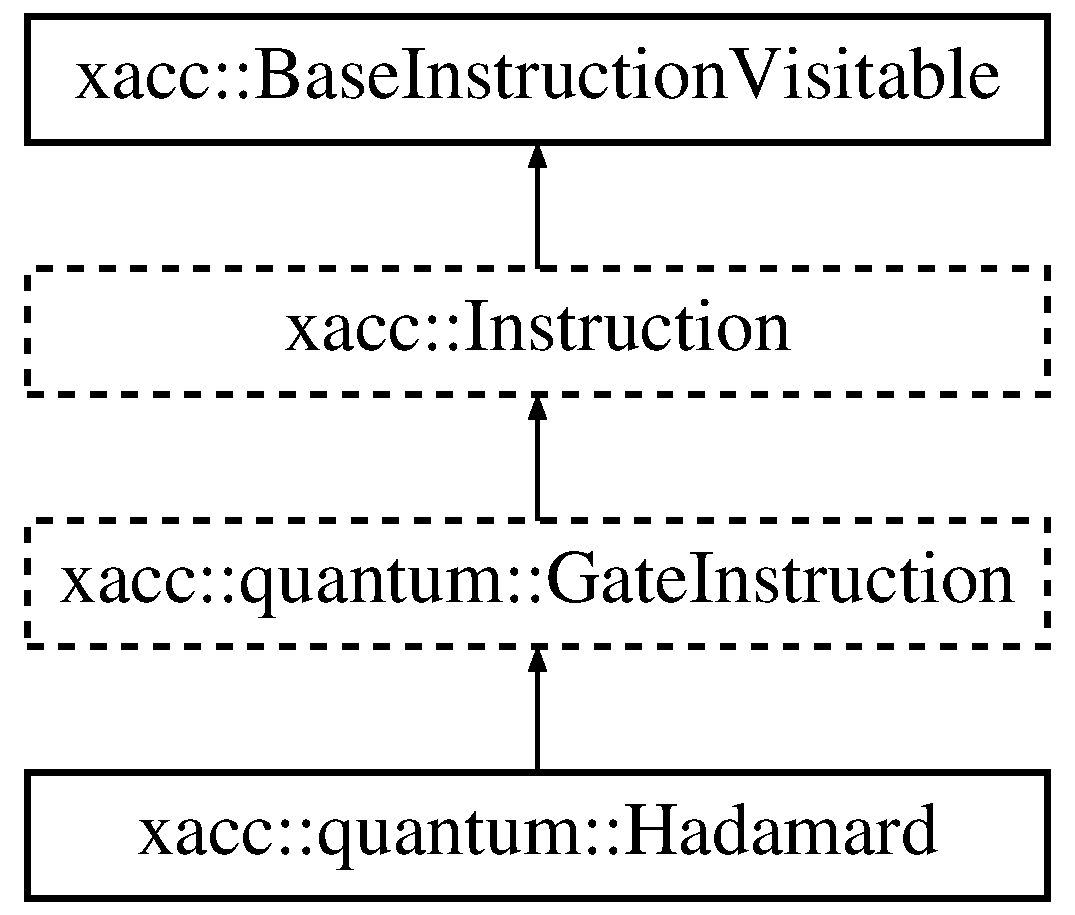
\includegraphics[height=4.000000cm]{a00044}
\end{center}
\end{figure}
\subsection*{Public Member Functions}
\begin{DoxyCompactItemize}
\item 
{\bfseries Hadamard} (std\+::vector$<$ int $>$ \hyperlink{a00041_a2a56be6c2519ea65df4d06f4abae1393}{qbits})\hypertarget{a00044_a1f26925eeb4a52ca7e52dd9158fe7005}{}\label{a00044_a1f26925eeb4a52ca7e52dd9158fe7005}

\item 
{\bfseries Hadamard} (int qbit)\hypertarget{a00044_aac4e06aae35583bcce39b6b178948364}{}\label{a00044_aac4e06aae35583bcce39b6b178948364}

\end{DoxyCompactItemize}
\subsection*{Additional Inherited Members}


The documentation for this class was generated from the following files\+:\begin{DoxyCompactItemize}
\item 
Hadamard.\+hpp\item 
Hadamard.\+cpp\end{DoxyCompactItemize}

\hypertarget{a00045}{}\section{xacc\+:\+:quantum\+:\+:H\+U\+BO$<$ Result\+Type $>$ Class Template Reference}
\label{a00045}\index{xacc\+::quantum\+::\+H\+U\+B\+O$<$ Result\+Type $>$@{xacc\+::quantum\+::\+H\+U\+B\+O$<$ Result\+Type $>$}}


{\ttfamily \#include $<$H\+U\+B\+O.\+hpp$>$}

\subsection*{Public Member Functions}
\begin{DoxyCompactItemize}
\item 
virtual std\+::shared\+\_\+ptr$<$ \hyperlink{a00030}{xacc\+::quantum\+::\+D\+W\+Graph} $>$ \hyperlink{a00045_ac1ef765d10ab355dd22d32e8259f0fea}{reduce\+To\+Qubo} (std\+::vector$<$ Instruction\+Parameter $>$ parameters)=0
\item 
virtual Result\+Type \hyperlink{a00045_a050aac403fabc54ff2726e28a8409194}{map\+Results} (std\+::shared\+\_\+ptr$<$ \hyperlink{a00013}{Accelerator\+Buffer} $>$ result\+Buffer)=0
\item 
virtual \hyperlink{a00045_a005d6122a7eb88fdd5889f154dc997bc}{$\sim$\+H\+U\+BO} ()
\end{DoxyCompactItemize}


\subsection{Detailed Description}
\subsubsection*{template$<$typename Result\+Type$>$\\*
class xacc\+::quantum\+::\+H\+U\+B\+O$<$ Result\+Type $>$}

\hyperlink{a00045}{H\+U\+BO} is an interface for higher-\/order unconstrained binary optimization problems. It provides a method for subclasses to implement that takes a set of input parameters and maps the problem down to a quadratic unconstrained binary optimization problem, in the form of a \hyperlink{a00043}{Graph}.

It takes a template parameter describing the return type of the map\+Results method -\/ which takes A\+QC Q\+PU execution results and maps them to the higher-\/order problem result. 

\subsection{Constructor \& Destructor Documentation}
\index{xacc\+::quantum\+::\+H\+U\+BO@{xacc\+::quantum\+::\+H\+U\+BO}!````~H\+U\+BO@{$\sim$\+H\+U\+BO}}
\index{````~H\+U\+BO@{$\sim$\+H\+U\+BO}!xacc\+::quantum\+::\+H\+U\+BO@{xacc\+::quantum\+::\+H\+U\+BO}}
\subsubsection[{\texorpdfstring{$\sim$\+H\+U\+B\+O()}{~HUBO()}}]{\setlength{\rightskip}{0pt plus 5cm}template$<$typename Result\+Type $>$ virtual {\bf xacc\+::quantum\+::\+H\+U\+BO}$<$ Result\+Type $>$\+::$\sim${\bf H\+U\+BO} (
\begin{DoxyParamCaption}
{}
\end{DoxyParamCaption}
)\hspace{0.3cm}{\ttfamily [inline]}, {\ttfamily [virtual]}}\hypertarget{a00045_a005d6122a7eb88fdd5889f154dc997bc}{}\label{a00045_a005d6122a7eb88fdd5889f154dc997bc}
The destructor 

\subsection{Member Function Documentation}
\index{xacc\+::quantum\+::\+H\+U\+BO@{xacc\+::quantum\+::\+H\+U\+BO}!map\+Results@{map\+Results}}
\index{map\+Results@{map\+Results}!xacc\+::quantum\+::\+H\+U\+BO@{xacc\+::quantum\+::\+H\+U\+BO}}
\subsubsection[{\texorpdfstring{map\+Results(std\+::shared\+\_\+ptr$<$ Accelerator\+Buffer $>$ result\+Buffer)=0}{mapResults(std::shared\_ptr< AcceleratorBuffer > resultBuffer)=0}}]{\setlength{\rightskip}{0pt plus 5cm}template$<$typename Result\+Type $>$ virtual Result\+Type {\bf xacc\+::quantum\+::\+H\+U\+BO}$<$ Result\+Type $>$\+::map\+Results (
\begin{DoxyParamCaption}
\item[{std\+::shared\+\_\+ptr$<$ {\bf Accelerator\+Buffer} $>$}]{result\+Buffer}
\end{DoxyParamCaption}
)\hspace{0.3cm}{\ttfamily [pure virtual]}}\hypertarget{a00045_a050aac403fabc54ff2726e28a8409194}{}\label{a00045_a050aac403fabc54ff2726e28a8409194}
Take the low-\/level A\+QC Q\+PU result output and construct result of \hyperlink{a00045}{H\+U\+BO} problem .


\begin{DoxyParams}{Parameters}
{\em result\+Buffer} & The \hyperlink{a00013}{Accelerator\+Buffer} containing the A\+QC Q\+PU results. \\
\hline
\end{DoxyParams}
\begin{DoxyReturn}{Returns}
results Custom Type representing the result. 
\end{DoxyReturn}
\index{xacc\+::quantum\+::\+H\+U\+BO@{xacc\+::quantum\+::\+H\+U\+BO}!reduce\+To\+Qubo@{reduce\+To\+Qubo}}
\index{reduce\+To\+Qubo@{reduce\+To\+Qubo}!xacc\+::quantum\+::\+H\+U\+BO@{xacc\+::quantum\+::\+H\+U\+BO}}
\subsubsection[{\texorpdfstring{reduce\+To\+Qubo(std\+::vector$<$ Instruction\+Parameter $>$ parameters)=0}{reduceToQubo(std::vector< InstructionParameter > parameters)=0}}]{\setlength{\rightskip}{0pt plus 5cm}template$<$typename Result\+Type $>$ virtual std\+::shared\+\_\+ptr$<${\bf xacc\+::quantum\+::\+D\+W\+Graph}$>$ {\bf xacc\+::quantum\+::\+H\+U\+BO}$<$ Result\+Type $>$\+::reduce\+To\+Qubo (
\begin{DoxyParamCaption}
\item[{std\+::vector$<$ Instruction\+Parameter $>$}]{parameters}
\end{DoxyParamCaption}
)\hspace{0.3cm}{\ttfamily [pure virtual]}}\hypertarget{a00045_ac1ef765d10ab355dd22d32e8259f0fea}{}\label{a00045_ac1ef765d10ab355dd22d32e8259f0fea}
Map this \hyperlink{a00045}{H\+U\+BO} problem to a quadratic unconstrained binary optimization problem.


\begin{DoxyParams}{Parameters}
{\em parameters} & Any input parameters needed to set the problem up \\
\hline
\end{DoxyParams}
\begin{DoxyReturn}{Returns}
qubo\+Graph The Q\+U\+BO represented as a graph 
\end{DoxyReturn}


The documentation for this class was generated from the following file\+:\begin{DoxyCompactItemize}
\item 
H\+U\+B\+O.\+hpp\end{DoxyCompactItemize}

\hypertarget{a00046}{}\section{xacc\+:\+:Instruction Class Reference}
\label{a00046}\index{xacc\+::\+Instruction@{xacc\+::\+Instruction}}


{\ttfamily \#include $<$Instruction.\+hpp$>$}

Inheritance diagram for xacc\+:\+:Instruction\+:\begin{figure}[H]
\begin{center}
\leavevmode
\includegraphics[height=10.370370cm]{a00046}
\end{center}
\end{figure}
\subsection*{Public Member Functions}
\begin{DoxyCompactItemize}
\item 
virtual const std\+::string \hyperlink{a00046_ac7ff23f693e2276edbf3fdac5452792c}{get\+Name} ()=0
\item 
virtual const std\+::string \hyperlink{a00046_ae94c2d089908294c1d410b14c96817ae}{to\+String} (const std\+::string \&buffer\+Var\+Name)=0
\item 
virtual const std\+::vector$<$ int $>$ \hyperlink{a00046_a819f32e94c3e1c9e69a0061aaf8d86dc}{bits} ()=0
\item 
virtual Instruction\+Parameter \hyperlink{a00046_aa0d9de97a4833a042379647f83c33ab6}{get\+Parameter} (const int idx)=0
\item 
virtual std\+::vector$<$ Instruction\+Parameter $>$ \hyperlink{a00046_aeb67c67713896e8f27a5c7dd531f3340}{get\+Parameters} ()=0
\item 
virtual void \hyperlink{a00046_a407a0ac662fa0b1ec3e301e8ff9bade7}{set\+Parameter} (const int idx, Instruction\+Parameter \&isnt)=0
\item 
virtual const int \hyperlink{a00046_ad54585d13c04ffd20296fff7ab8107ff}{n\+Parameters} ()=0
\item 
virtual bool \hyperlink{a00046_a7b24d8ae485369fc2b2df7a3224a5e26}{is\+Parameterized} ()
\item 
virtual bool \hyperlink{a00046_a4383f1036d0fcfe890ab9c613dbd5f38}{is\+Composite} ()
\item 
virtual bool \hyperlink{a00046_ad02a1cf7220577124720b7a51424cea7}{is\+Enabled} ()
\item 
virtual void \hyperlink{a00046_a6e528da15e05a94cc1d7db268c483271}{disable} ()
\item 
virtual void \hyperlink{a00046_a0b4f2e5a591af28342a3c08e4305e24f}{enable} ()
\item 
virtual \hyperlink{a00046_ae22c935e8113bce63d1d0e214cda4d61}{$\sim$\+Instruction} ()
\end{DoxyCompactItemize}
\subsection*{Additional Inherited Members}


\subsection{Detailed Description}
The \hyperlink{a00046}{Instruction} interface is the base of all X\+A\+CC Intermediate Representation Instructions for post-\/\+Moore\textquotesingle{}s law accelerated computing. The \hyperlink{a00046}{Instruction}, at its core, provides an \hyperlink{a00046}{Instruction} name and a set of next-\/gen bits that the \hyperlink{a00046}{Instruction} operates on. Instructions can also be enabled or disabled. Instructions implement \hyperlink{a00017}{Base\+Instruction\+Visitable} to enable visitor pattern functionality across all \hyperlink{a00046}{Instruction} subclasses.

\hyperlink{a00046}{Instruction} can also expose 0 to N Instruction\+Parameters. Instruction\+Parameters can be an int, double, float, or string. 

\subsection{Constructor \& Destructor Documentation}
\index{xacc\+::\+Instruction@{xacc\+::\+Instruction}!````~Instruction@{$\sim$\+Instruction}}
\index{````~Instruction@{$\sim$\+Instruction}!xacc\+::\+Instruction@{xacc\+::\+Instruction}}
\subsubsection[{\texorpdfstring{$\sim$\+Instruction()}{~Instruction()}}]{\setlength{\rightskip}{0pt plus 5cm}virtual xacc\+::\+Instruction\+::$\sim$\+Instruction (
\begin{DoxyParamCaption}
{}
\end{DoxyParamCaption}
)\hspace{0.3cm}{\ttfamily [inline]}, {\ttfamily [virtual]}}\hypertarget{a00046_ae22c935e8113bce63d1d0e214cda4d61}{}\label{a00046_ae22c935e8113bce63d1d0e214cda4d61}
The destructor 

\subsection{Member Function Documentation}
\index{xacc\+::\+Instruction@{xacc\+::\+Instruction}!bits@{bits}}
\index{bits@{bits}!xacc\+::\+Instruction@{xacc\+::\+Instruction}}
\subsubsection[{\texorpdfstring{bits()=0}{bits()=0}}]{\setlength{\rightskip}{0pt plus 5cm}virtual const std\+::vector$<$int$>$ xacc\+::\+Instruction\+::bits (
\begin{DoxyParamCaption}
{}
\end{DoxyParamCaption}
)\hspace{0.3cm}{\ttfamily [pure virtual]}}\hypertarget{a00046_a819f32e94c3e1c9e69a0061aaf8d86dc}{}\label{a00046_a819f32e94c3e1c9e69a0061aaf8d86dc}
Return the indices of the bits that this \hyperlink{a00046}{Instruction} operates on.

\begin{DoxyReturn}{Returns}
bits The bits this \hyperlink{a00046}{Instruction} operates on. 
\end{DoxyReturn}


Implemented in \hyperlink{a00040_aba03de68b76a9e120705c3c389c714a1}{xacc\+::quantum\+::\+Gate\+Function}, \hyperlink{a00033_a76939c29e4763d10c57ea9a270229421}{xacc\+::quantum\+::\+D\+W\+Q\+MI}, \hyperlink{a00032_adae68964db6acd8b4c2267c270a8ec58}{xacc\+::quantum\+::\+D\+W\+Kernel}, and \hyperlink{a00041_ad32ad03dfc516e00093030e60178003d}{xacc\+::quantum\+::\+Gate\+Instruction}.

\index{xacc\+::\+Instruction@{xacc\+::\+Instruction}!disable@{disable}}
\index{disable@{disable}!xacc\+::\+Instruction@{xacc\+::\+Instruction}}
\subsubsection[{\texorpdfstring{disable()}{disable()}}]{\setlength{\rightskip}{0pt plus 5cm}virtual void xacc\+::\+Instruction\+::disable (
\begin{DoxyParamCaption}
{}
\end{DoxyParamCaption}
)\hspace{0.3cm}{\ttfamily [inline]}, {\ttfamily [virtual]}}\hypertarget{a00046_a6e528da15e05a94cc1d7db268c483271}{}\label{a00046_a6e528da15e05a94cc1d7db268c483271}
Disable this \hyperlink{a00046}{Instruction} 

Reimplemented in \hyperlink{a00033_af6d9120d8f60984767a330d5cfe9140f}{xacc\+::quantum\+::\+D\+W\+Q\+MI}, and \hyperlink{a00041_a63ce138dd71fb43d303f5600fefb7215}{xacc\+::quantum\+::\+Gate\+Instruction}.

\index{xacc\+::\+Instruction@{xacc\+::\+Instruction}!enable@{enable}}
\index{enable@{enable}!xacc\+::\+Instruction@{xacc\+::\+Instruction}}
\subsubsection[{\texorpdfstring{enable()}{enable()}}]{\setlength{\rightskip}{0pt plus 5cm}virtual void xacc\+::\+Instruction\+::enable (
\begin{DoxyParamCaption}
{}
\end{DoxyParamCaption}
)\hspace{0.3cm}{\ttfamily [inline]}, {\ttfamily [virtual]}}\hypertarget{a00046_a0b4f2e5a591af28342a3c08e4305e24f}{}\label{a00046_a0b4f2e5a591af28342a3c08e4305e24f}
Enable this \hyperlink{a00046}{Instruction}. 

Reimplemented in \hyperlink{a00033_ae4f563cead75aaa43f06db83e90ee855}{xacc\+::quantum\+::\+D\+W\+Q\+MI}, and \hyperlink{a00041_a7a80474b7fd465271b3313432db2e608}{xacc\+::quantum\+::\+Gate\+Instruction}.

\index{xacc\+::\+Instruction@{xacc\+::\+Instruction}!get\+Name@{get\+Name}}
\index{get\+Name@{get\+Name}!xacc\+::\+Instruction@{xacc\+::\+Instruction}}
\subsubsection[{\texorpdfstring{get\+Name()=0}{getName()=0}}]{\setlength{\rightskip}{0pt plus 5cm}virtual const std\+::string xacc\+::\+Instruction\+::get\+Name (
\begin{DoxyParamCaption}
{}
\end{DoxyParamCaption}
)\hspace{0.3cm}{\ttfamily [pure virtual]}}\hypertarget{a00046_ac7ff23f693e2276edbf3fdac5452792c}{}\label{a00046_ac7ff23f693e2276edbf3fdac5452792c}
Return the name of this \hyperlink{a00046}{Instruction}

\begin{DoxyReturn}{Returns}
name The name of this \hyperlink{a00046}{Instruction} 
\end{DoxyReturn}


Implemented in \hyperlink{a00040_af42efb6191267164717d53c469e15d3a}{xacc\+::quantum\+::\+Gate\+Function}, \hyperlink{a00032_a7f0c4d3c73029566561cf56a474bcbbd}{xacc\+::quantum\+::\+D\+W\+Kernel}, \hyperlink{a00033_ad93428eb61adade7bb99c7633bb02aca}{xacc\+::quantum\+::\+D\+W\+Q\+MI}, and \hyperlink{a00041_a0db03b9e46eeba1134f0ca2b83ccc842}{xacc\+::quantum\+::\+Gate\+Instruction}.

\index{xacc\+::\+Instruction@{xacc\+::\+Instruction}!get\+Parameter@{get\+Parameter}}
\index{get\+Parameter@{get\+Parameter}!xacc\+::\+Instruction@{xacc\+::\+Instruction}}
\subsubsection[{\texorpdfstring{get\+Parameter(const int idx)=0}{getParameter(const int idx)=0}}]{\setlength{\rightskip}{0pt plus 5cm}virtual Instruction\+Parameter xacc\+::\+Instruction\+::get\+Parameter (
\begin{DoxyParamCaption}
\item[{const int}]{idx}
\end{DoxyParamCaption}
)\hspace{0.3cm}{\ttfamily [pure virtual]}}\hypertarget{a00046_aa0d9de97a4833a042379647f83c33ab6}{}\label{a00046_aa0d9de97a4833a042379647f83c33ab6}
Return this \hyperlink{a00046}{Instruction}\textquotesingle{}s parameter at the given index.


\begin{DoxyParams}{Parameters}
{\em idx} & The index of the parameter. \\
\hline
\end{DoxyParams}
\begin{DoxyReturn}{Returns}
param The Instruction\+Parameter at the given index. 
\end{DoxyReturn}


Implemented in \hyperlink{a00032_a81711b7db284aba35d6952e4d1d15d41}{xacc\+::quantum\+::\+D\+W\+Kernel}, \hyperlink{a00040_a5991903323e412777bedc4f0c862eb63}{xacc\+::quantum\+::\+Gate\+Function}, \hyperlink{a00033_aa15882df55d3f0af3a2ec9d72a2db4c0}{xacc\+::quantum\+::\+D\+W\+Q\+MI}, and \hyperlink{a00041_addd6185279fe99fbdc3d4efd96e42162}{xacc\+::quantum\+::\+Gate\+Instruction}.

\index{xacc\+::\+Instruction@{xacc\+::\+Instruction}!get\+Parameters@{get\+Parameters}}
\index{get\+Parameters@{get\+Parameters}!xacc\+::\+Instruction@{xacc\+::\+Instruction}}
\subsubsection[{\texorpdfstring{get\+Parameters()=0}{getParameters()=0}}]{\setlength{\rightskip}{0pt plus 5cm}virtual std\+::vector$<$Instruction\+Parameter$>$ xacc\+::\+Instruction\+::get\+Parameters (
\begin{DoxyParamCaption}
{}
\end{DoxyParamCaption}
)\hspace{0.3cm}{\ttfamily [pure virtual]}}\hypertarget{a00046_aeb67c67713896e8f27a5c7dd531f3340}{}\label{a00046_aeb67c67713896e8f27a5c7dd531f3340}
Return all of this \hyperlink{a00046}{Instruction}\textquotesingle{}s parameters.

\begin{DoxyReturn}{Returns}
params This instructions parameters. 
\end{DoxyReturn}


Implemented in \hyperlink{a00040_af7aabfe699a4dced576ff7fafff969d5}{xacc\+::quantum\+::\+Gate\+Function}, \hyperlink{a00032_a829462cff34e2257da06afd8a2051a8e}{xacc\+::quantum\+::\+D\+W\+Kernel}, \hyperlink{a00041_a8584444f9577283f6844ab32bdc4db72}{xacc\+::quantum\+::\+Gate\+Instruction}, and \hyperlink{a00033_a896d9a4e2876129c2cf81ef028daf1ff}{xacc\+::quantum\+::\+D\+W\+Q\+MI}.

\index{xacc\+::\+Instruction@{xacc\+::\+Instruction}!is\+Composite@{is\+Composite}}
\index{is\+Composite@{is\+Composite}!xacc\+::\+Instruction@{xacc\+::\+Instruction}}
\subsubsection[{\texorpdfstring{is\+Composite()}{isComposite()}}]{\setlength{\rightskip}{0pt plus 5cm}virtual bool xacc\+::\+Instruction\+::is\+Composite (
\begin{DoxyParamCaption}
{}
\end{DoxyParamCaption}
)\hspace{0.3cm}{\ttfamily [inline]}, {\ttfamily [virtual]}}\hypertarget{a00046_a4383f1036d0fcfe890ab9c613dbd5f38}{}\label{a00046_a4383f1036d0fcfe890ab9c613dbd5f38}
Returns true if this \hyperlink{a00046}{Instruction} is composite, ie, contains other Instructions.

\begin{DoxyReturn}{Returns}
is\+Composite True if this is a composite \hyperlink{a00046}{Instruction} 
\end{DoxyReturn}


Reimplemented in \hyperlink{a00033_ad2b3b4ee72dee48150bf78d92c52e5e0}{xacc\+::quantum\+::\+D\+W\+Q\+MI}, and \hyperlink{a00038_aa75500c657b5c3e0e36213e1506aad97}{xacc\+::\+Function}.

\index{xacc\+::\+Instruction@{xacc\+::\+Instruction}!is\+Enabled@{is\+Enabled}}
\index{is\+Enabled@{is\+Enabled}!xacc\+::\+Instruction@{xacc\+::\+Instruction}}
\subsubsection[{\texorpdfstring{is\+Enabled()}{isEnabled()}}]{\setlength{\rightskip}{0pt plus 5cm}virtual bool xacc\+::\+Instruction\+::is\+Enabled (
\begin{DoxyParamCaption}
{}
\end{DoxyParamCaption}
)\hspace{0.3cm}{\ttfamily [inline]}, {\ttfamily [virtual]}}\hypertarget{a00046_ad02a1cf7220577124720b7a51424cea7}{}\label{a00046_ad02a1cf7220577124720b7a51424cea7}
Returns true if this \hyperlink{a00046}{Instruction} is enabled

\begin{DoxyReturn}{Returns}
enabled True if this \hyperlink{a00046}{Instruction} is enabled. 
\end{DoxyReturn}


Reimplemented in \hyperlink{a00033_aea76901b30d85172ef26fc317b4c0ed7}{xacc\+::quantum\+::\+D\+W\+Q\+MI}, and \hyperlink{a00041_a0a821be322b0c848b01c55f91fc8f484}{xacc\+::quantum\+::\+Gate\+Instruction}.

\index{xacc\+::\+Instruction@{xacc\+::\+Instruction}!is\+Parameterized@{is\+Parameterized}}
\index{is\+Parameterized@{is\+Parameterized}!xacc\+::\+Instruction@{xacc\+::\+Instruction}}
\subsubsection[{\texorpdfstring{is\+Parameterized()}{isParameterized()}}]{\setlength{\rightskip}{0pt plus 5cm}virtual bool xacc\+::\+Instruction\+::is\+Parameterized (
\begin{DoxyParamCaption}
{}
\end{DoxyParamCaption}
)\hspace{0.3cm}{\ttfamily [inline]}, {\ttfamily [virtual]}}\hypertarget{a00046_a7b24d8ae485369fc2b2df7a3224a5e26}{}\label{a00046_a7b24d8ae485369fc2b2df7a3224a5e26}
Return true if this \hyperlink{a00046}{Instruction} is parameterized.

\begin{DoxyReturn}{Returns}
parameterized True if this \hyperlink{a00046}{Instruction} has parameters. 
\end{DoxyReturn}


Reimplemented in \hyperlink{a00033_aee43b2e499f122dfe250b529a3f77add}{xacc\+::quantum\+::\+D\+W\+Q\+MI}, \hyperlink{a00040_afad47903e0ed55ddbfa827ef8408a94b}{xacc\+::quantum\+::\+Gate\+Function}, \hyperlink{a00032_a8957ea368244ed4a4ebd85f6bfecb785}{xacc\+::quantum\+::\+D\+W\+Kernel}, and \hyperlink{a00041_afe7aeeb398262931e156bcb3950f8188}{xacc\+::quantum\+::\+Gate\+Instruction}.

\index{xacc\+::\+Instruction@{xacc\+::\+Instruction}!n\+Parameters@{n\+Parameters}}
\index{n\+Parameters@{n\+Parameters}!xacc\+::\+Instruction@{xacc\+::\+Instruction}}
\subsubsection[{\texorpdfstring{n\+Parameters()=0}{nParameters()=0}}]{\setlength{\rightskip}{0pt plus 5cm}virtual const int xacc\+::\+Instruction\+::n\+Parameters (
\begin{DoxyParamCaption}
{}
\end{DoxyParamCaption}
)\hspace{0.3cm}{\ttfamily [pure virtual]}}\hypertarget{a00046_ad54585d13c04ffd20296fff7ab8107ff}{}\label{a00046_ad54585d13c04ffd20296fff7ab8107ff}
Return the number of Instruction\+Parameters this \hyperlink{a00046}{Instruction} contains.

\begin{DoxyReturn}{Returns}
n\+Insts The number of instructions. 
\end{DoxyReturn}


Implemented in \hyperlink{a00040_ad0bffcbc0884d81d6bdddf55385fc6c9}{xacc\+::quantum\+::\+Gate\+Function}, \hyperlink{a00032_a029429948329b94c1d89f32cf5c486d4}{xacc\+::quantum\+::\+D\+W\+Kernel}, \hyperlink{a00033_afdfc8b852ba29c2b21c5c368098ffc4c}{xacc\+::quantum\+::\+D\+W\+Q\+MI}, and \hyperlink{a00041_a3752912b2c402668ca4814e21d4bbd26}{xacc\+::quantum\+::\+Gate\+Instruction}.

\index{xacc\+::\+Instruction@{xacc\+::\+Instruction}!set\+Parameter@{set\+Parameter}}
\index{set\+Parameter@{set\+Parameter}!xacc\+::\+Instruction@{xacc\+::\+Instruction}}
\subsubsection[{\texorpdfstring{set\+Parameter(const int idx, Instruction\+Parameter \&isnt)=0}{setParameter(const int idx, InstructionParameter \&isnt)=0}}]{\setlength{\rightskip}{0pt plus 5cm}virtual void xacc\+::\+Instruction\+::set\+Parameter (
\begin{DoxyParamCaption}
\item[{const int}]{idx, }
\item[{Instruction\+Parameter \&}]{isnt}
\end{DoxyParamCaption}
)\hspace{0.3cm}{\ttfamily [pure virtual]}}\hypertarget{a00046_a407a0ac662fa0b1ec3e301e8ff9bade7}{}\label{a00046_a407a0ac662fa0b1ec3e301e8ff9bade7}
Set this \hyperlink{a00046}{Instruction}\textquotesingle{}s parameter at the given index.


\begin{DoxyParams}{Parameters}
{\em idx} & The index of the parameter \\
\hline
{\em inst} & The instruction. \\
\hline
\end{DoxyParams}


Implemented in \hyperlink{a00032_adf89cdd1f54e183c4cff36b338b2be8d}{xacc\+::quantum\+::\+D\+W\+Kernel}, \hyperlink{a00040_ab8d9789b46e92e27a9d7c9c5b7e3683c}{xacc\+::quantum\+::\+Gate\+Function}, \hyperlink{a00033_a194b5b9f58262774fde0285f4c3f60af}{xacc\+::quantum\+::\+D\+W\+Q\+MI}, and \hyperlink{a00041_afb8f7582d7520c77d61b9016753f5669}{xacc\+::quantum\+::\+Gate\+Instruction}.

\index{xacc\+::\+Instruction@{xacc\+::\+Instruction}!to\+String@{to\+String}}
\index{to\+String@{to\+String}!xacc\+::\+Instruction@{xacc\+::\+Instruction}}
\subsubsection[{\texorpdfstring{to\+String(const std\+::string \&buffer\+Var\+Name)=0}{toString(const std::string \&bufferVarName)=0}}]{\setlength{\rightskip}{0pt plus 5cm}virtual const std\+::string xacc\+::\+Instruction\+::to\+String (
\begin{DoxyParamCaption}
\item[{const std\+::string \&}]{buffer\+Var\+Name}
\end{DoxyParamCaption}
)\hspace{0.3cm}{\ttfamily [pure virtual]}}\hypertarget{a00046_ae94c2d089908294c1d410b14c96817ae}{}\label{a00046_ae94c2d089908294c1d410b14c96817ae}
Persist this \hyperlink{a00046}{Instruction} to an assembly-\/like string.


\begin{DoxyParams}{Parameters}
{\em buffer\+Var\+Name} & The name of the \hyperlink{a00013}{Accelerator\+Buffer} \\
\hline
\end{DoxyParams}
\begin{DoxyReturn}{Returns}
str The assembly-\/like string. 
\end{DoxyReturn}


Implemented in \hyperlink{a00040_aa1950776ae84bad2d0795a0441f910e7}{xacc\+::quantum\+::\+Gate\+Function}, \hyperlink{a00032_adbc3fdd080ebba20bc620b8832979f16}{xacc\+::quantum\+::\+D\+W\+Kernel}, \hyperlink{a00033_a8d8742bb6743cf6e49f95966d05bbec2}{xacc\+::quantum\+::\+D\+W\+Q\+MI}, \hyperlink{a00041_a089a5da67ff40ac1a6f56e64589822d9}{xacc\+::quantum\+::\+Gate\+Instruction}, \hyperlink{a00055_a1c51a5d68294dcb2ba1a9fbea63a730f}{xacc\+::quantum\+::\+Measure}, and \hyperlink{a00025_aca7a5f849fece6fc28a904efee9a3370}{xacc\+::quantum\+::\+Conditional\+Function}.



The documentation for this class was generated from the following file\+:\begin{DoxyCompactItemize}
\item 
Instruction.\+hpp\end{DoxyCompactItemize}

\hypertarget{a00047}{}\section{xacc\+:\+:Instruction\+Iterator Class Reference}
\label{a00047}\index{xacc\+::\+Instruction\+Iterator@{xacc\+::\+Instruction\+Iterator}}


{\ttfamily \#include $<$Instruction\+Iterator.\+hpp$>$}

\subsection*{Public Member Functions}
\begin{DoxyCompactItemize}
\item 
\hyperlink{a00047_af61abf612341ab1454a1c43239b2da16}{Instruction\+Iterator} (std\+::shared\+\_\+ptr$<$ \hyperlink{a00046}{Instruction} $>$ r)
\item 
bool \hyperlink{a00047_a7fa6c8cff43e7b224211d4f7954a4152}{has\+Next} ()
\item 
std\+::shared\+\_\+ptr$<$ \hyperlink{a00046}{Instruction} $>$ \hyperlink{a00047_a0a2e2b1543650760a869460ebcd4382b}{next} ()
\end{DoxyCompactItemize}
\subsection*{Protected Attributes}
\begin{DoxyCompactItemize}
\item 
std\+::shared\+\_\+ptr$<$ \hyperlink{a00046}{Instruction} $>$ \hyperlink{a00047_a9d7aee1cb9058dd4a29c8fc71eeda57d}{root}
\item 
std\+::stack$<$ std\+::shared\+\_\+ptr$<$ \hyperlink{a00046}{Instruction} $>$ $>$ \hyperlink{a00047_a7af48509e563e8865131692c3b71edf0}{inst\+Stack}
\end{DoxyCompactItemize}


\subsection{Detailed Description}
The \hyperlink{a00047}{Instruction\+Iterator} provides a mechanism for a pre-\/order traversal of an \hyperlink{a00046}{Instruction} tree. 

\subsection{Constructor \& Destructor Documentation}
\index{xacc\+::\+Instruction\+Iterator@{xacc\+::\+Instruction\+Iterator}!Instruction\+Iterator@{Instruction\+Iterator}}
\index{Instruction\+Iterator@{Instruction\+Iterator}!xacc\+::\+Instruction\+Iterator@{xacc\+::\+Instruction\+Iterator}}
\subsubsection[{\texorpdfstring{Instruction\+Iterator(std\+::shared\+\_\+ptr$<$ Instruction $>$ r)}{InstructionIterator(std::shared\_ptr< Instruction > r)}}]{\setlength{\rightskip}{0pt plus 5cm}xacc\+::\+Instruction\+Iterator\+::\+Instruction\+Iterator (
\begin{DoxyParamCaption}
\item[{std\+::shared\+\_\+ptr$<$ {\bf Instruction} $>$}]{r}
\end{DoxyParamCaption}
)\hspace{0.3cm}{\ttfamily [inline]}}\hypertarget{a00047_af61abf612341ab1454a1c43239b2da16}{}\label{a00047_af61abf612341ab1454a1c43239b2da16}
The constructor, takes the root of the tree as input.


\begin{DoxyParams}{Parameters}
{\em r} & \\
\hline
\end{DoxyParams}


\subsection{Member Function Documentation}
\index{xacc\+::\+Instruction\+Iterator@{xacc\+::\+Instruction\+Iterator}!has\+Next@{has\+Next}}
\index{has\+Next@{has\+Next}!xacc\+::\+Instruction\+Iterator@{xacc\+::\+Instruction\+Iterator}}
\subsubsection[{\texorpdfstring{has\+Next()}{hasNext()}}]{\setlength{\rightskip}{0pt plus 5cm}bool xacc\+::\+Instruction\+Iterator\+::has\+Next (
\begin{DoxyParamCaption}
{}
\end{DoxyParamCaption}
)\hspace{0.3cm}{\ttfamily [inline]}}\hypertarget{a00047_a7fa6c8cff43e7b224211d4f7954a4152}{}\label{a00047_a7fa6c8cff43e7b224211d4f7954a4152}
Return true if there are still instructions left to traverse. \begin{DoxyReturn}{Returns}

\end{DoxyReturn}
\index{xacc\+::\+Instruction\+Iterator@{xacc\+::\+Instruction\+Iterator}!next@{next}}
\index{next@{next}!xacc\+::\+Instruction\+Iterator@{xacc\+::\+Instruction\+Iterator}}
\subsubsection[{\texorpdfstring{next()}{next()}}]{\setlength{\rightskip}{0pt plus 5cm}std\+::shared\+\_\+ptr$<${\bf Instruction}$>$ xacc\+::\+Instruction\+Iterator\+::next (
\begin{DoxyParamCaption}
{}
\end{DoxyParamCaption}
)\hspace{0.3cm}{\ttfamily [inline]}}\hypertarget{a00047_a0a2e2b1543650760a869460ebcd4382b}{}\label{a00047_a0a2e2b1543650760a869460ebcd4382b}
Return the next \hyperlink{a00046}{Instruction} in the tree. \begin{DoxyReturn}{Returns}

\end{DoxyReturn}


\subsection{Member Data Documentation}
\index{xacc\+::\+Instruction\+Iterator@{xacc\+::\+Instruction\+Iterator}!inst\+Stack@{inst\+Stack}}
\index{inst\+Stack@{inst\+Stack}!xacc\+::\+Instruction\+Iterator@{xacc\+::\+Instruction\+Iterator}}
\subsubsection[{\texorpdfstring{inst\+Stack}{instStack}}]{\setlength{\rightskip}{0pt plus 5cm}std\+::stack$<$std\+::shared\+\_\+ptr$<${\bf Instruction}$>$ $>$ xacc\+::\+Instruction\+Iterator\+::inst\+Stack\hspace{0.3cm}{\ttfamily [protected]}}\hypertarget{a00047_a7af48509e563e8865131692c3b71edf0}{}\label{a00047_a7af48509e563e8865131692c3b71edf0}
A stack used to implement the tree traversal \index{xacc\+::\+Instruction\+Iterator@{xacc\+::\+Instruction\+Iterator}!root@{root}}
\index{root@{root}!xacc\+::\+Instruction\+Iterator@{xacc\+::\+Instruction\+Iterator}}
\subsubsection[{\texorpdfstring{root}{root}}]{\setlength{\rightskip}{0pt plus 5cm}std\+::shared\+\_\+ptr$<${\bf Instruction}$>$ xacc\+::\+Instruction\+Iterator\+::root\hspace{0.3cm}{\ttfamily [protected]}}\hypertarget{a00047_a9d7aee1cb9058dd4a29c8fc71eeda57d}{}\label{a00047_a9d7aee1cb9058dd4a29c8fc71eeda57d}
The root of the tree, a function 

The documentation for this class was generated from the following file\+:\begin{DoxyCompactItemize}
\item 
Instruction\+Iterator.\+hpp\end{DoxyCompactItemize}

\hypertarget{a00048}{}\section{xacc\+:\+:Instruction\+Visitor$<$ T $>$ Class Template Reference}
\label{a00048}\index{xacc\+::\+Instruction\+Visitor$<$ T $>$@{xacc\+::\+Instruction\+Visitor$<$ T $>$}}


{\ttfamily \#include $<$Instruction\+Visitor.\+hpp$>$}

\subsection*{Public Member Functions}
\begin{DoxyCompactItemize}
\item 
virtual void \hyperlink{a00048_af0fead298f5bfbb8e6680433063e2c4b}{visit} (T \&)=0
\item 
virtual \hyperlink{a00048_adf624df25964d0be1a56af58639c9e1d}{$\sim$\+Instruction\+Visitor} ()
\end{DoxyCompactItemize}


\subsection{Detailed Description}
\subsubsection*{template$<$class T$>$\\*
class xacc\+::\+Instruction\+Visitor$<$ T $>$}

The \hyperlink{a00048}{Instruction\+Visitor} provides a visit method for the provided template parameter. 

\subsection{Constructor \& Destructor Documentation}
\index{xacc\+::\+Instruction\+Visitor@{xacc\+::\+Instruction\+Visitor}!````~Instruction\+Visitor@{$\sim$\+Instruction\+Visitor}}
\index{````~Instruction\+Visitor@{$\sim$\+Instruction\+Visitor}!xacc\+::\+Instruction\+Visitor@{xacc\+::\+Instruction\+Visitor}}
\subsubsection[{\texorpdfstring{$\sim$\+Instruction\+Visitor()}{~InstructionVisitor()}}]{\setlength{\rightskip}{0pt plus 5cm}template$<$class T$>$ virtual {\bf xacc\+::\+Instruction\+Visitor}$<$ T $>$\+::$\sim${\bf Instruction\+Visitor} (
\begin{DoxyParamCaption}
{}
\end{DoxyParamCaption}
)\hspace{0.3cm}{\ttfamily [inline]}, {\ttfamily [virtual]}}\hypertarget{a00048_adf624df25964d0be1a56af58639c9e1d}{}\label{a00048_adf624df25964d0be1a56af58639c9e1d}
The destructor 

\subsection{Member Function Documentation}
\index{xacc\+::\+Instruction\+Visitor@{xacc\+::\+Instruction\+Visitor}!visit@{visit}}
\index{visit@{visit}!xacc\+::\+Instruction\+Visitor@{xacc\+::\+Instruction\+Visitor}}
\subsubsection[{\texorpdfstring{visit(\+T \&)=0}{visit(T \&)=0}}]{\setlength{\rightskip}{0pt plus 5cm}template$<$class T$>$ virtual void {\bf xacc\+::\+Instruction\+Visitor}$<$ T $>$\+::visit (
\begin{DoxyParamCaption}
\item[{T \&}]{}
\end{DoxyParamCaption}
)\hspace{0.3cm}{\ttfamily [pure virtual]}}\hypertarget{a00048_af0fead298f5bfbb8e6680433063e2c4b}{}\label{a00048_af0fead298f5bfbb8e6680433063e2c4b}
This method should be implemented by subclasses to perform Visitor-\/specific behavior on the given instance of the template parameter T. 

Implemented in \hyperlink{a00026_a9c40e6cb4b74e2d6714c531ffc3b2909}{xacc\+::quantum\+::\+Count\+Gates\+Of\+Type\+Visitor$<$ Gate\+Type $>$}.



The documentation for this class was generated from the following file\+:\begin{DoxyCompactItemize}
\item 
Instruction\+Visitor.\+hpp\end{DoxyCompactItemize}

\hypertarget{a00049}{}\section{xacc\+:\+:quantum\+:\+:Inverse\+Q\+FT Class Reference}
\label{a00049}\index{xacc\+::quantum\+::\+Inverse\+Q\+FT@{xacc\+::quantum\+::\+Inverse\+Q\+FT}}


{\ttfamily \#include $<$Inverse\+Q\+F\+T.\+hpp$>$}

Inheritance diagram for xacc\+:\+:quantum\+:\+:Inverse\+Q\+FT\+:\begin{figure}[H]
\begin{center}
\leavevmode
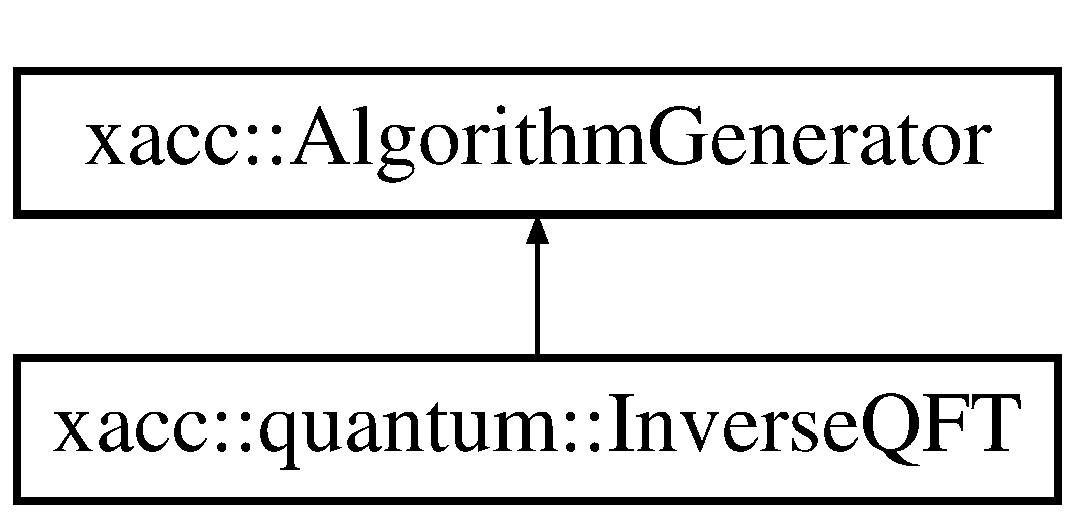
\includegraphics[height=2.000000cm]{a00049}
\end{center}
\end{figure}
\subsection*{Public Member Functions}
\begin{DoxyCompactItemize}
\item 
virtual std\+::shared\+\_\+ptr$<$ \hyperlink{a00038}{Function} $>$ \hyperlink{a00049_af42e466bf02dbd60670d20aa55cfb08d}{generate\+Algorithm} (std\+::vector$<$ int $>$ qubits)
\item 
virtual \hyperlink{a00049_a731c10d28046424be74e4c0daa31d016}{$\sim$\+Inverse\+Q\+FT} ()
\end{DoxyCompactItemize}


\subsection{Detailed Description}
\hyperlink{a00049}{Inverse\+Q\+FT} is a realization of the \hyperlink{a00014}{Algorithm\+Generator} interface that produces an X\+A\+CC \hyperlink{a00050}{IR} representation of the Inverse Quantum Fourier Transform. 

\subsection{Constructor \& Destructor Documentation}
\index{xacc\+::quantum\+::\+Inverse\+Q\+FT@{xacc\+::quantum\+::\+Inverse\+Q\+FT}!````~Inverse\+Q\+FT@{$\sim$\+Inverse\+Q\+FT}}
\index{````~Inverse\+Q\+FT@{$\sim$\+Inverse\+Q\+FT}!xacc\+::quantum\+::\+Inverse\+Q\+FT@{xacc\+::quantum\+::\+Inverse\+Q\+FT}}
\subsubsection[{\texorpdfstring{$\sim$\+Inverse\+Q\+F\+T()}{~InverseQFT()}}]{\setlength{\rightskip}{0pt plus 5cm}virtual xacc\+::quantum\+::\+Inverse\+Q\+F\+T\+::$\sim$\+Inverse\+Q\+FT (
\begin{DoxyParamCaption}
{}
\end{DoxyParamCaption}
)\hspace{0.3cm}{\ttfamily [inline]}, {\ttfamily [virtual]}}\hypertarget{a00049_a731c10d28046424be74e4c0daa31d016}{}\label{a00049_a731c10d28046424be74e4c0daa31d016}
The destructor 

\subsection{Member Function Documentation}
\index{xacc\+::quantum\+::\+Inverse\+Q\+FT@{xacc\+::quantum\+::\+Inverse\+Q\+FT}!generate\+Algorithm@{generate\+Algorithm}}
\index{generate\+Algorithm@{generate\+Algorithm}!xacc\+::quantum\+::\+Inverse\+Q\+FT@{xacc\+::quantum\+::\+Inverse\+Q\+FT}}
\subsubsection[{\texorpdfstring{generate\+Algorithm(std\+::vector$<$ int $>$ qubits)}{generateAlgorithm(std::vector< int > qubits)}}]{\setlength{\rightskip}{0pt plus 5cm}std\+::shared\+\_\+ptr$<$ {\bf Function} $>$ xacc\+::quantum\+::\+Inverse\+Q\+F\+T\+::generate\+Algorithm (
\begin{DoxyParamCaption}
\item[{std\+::vector$<$ int $>$}]{qubits}
\end{DoxyParamCaption}
)\hspace{0.3cm}{\ttfamily [virtual]}}\hypertarget{a00049_af42e466bf02dbd60670d20aa55cfb08d}{}\label{a00049_af42e466bf02dbd60670d20aa55cfb08d}
This implementation returns a \hyperlink{a00038}{Function} \hyperlink{a00050}{IR} representation of the inverse quantum fourier transform.


\begin{DoxyParams}{Parameters}
{\em bits} & The bits this algorithm operates on \\
\hline
\end{DoxyParams}
\begin{DoxyReturn}{Returns}
function The algorithm represented as an \hyperlink{a00050}{IR} \hyperlink{a00038}{Function} 
\end{DoxyReturn}


Implements \hyperlink{a00014_a73023c06f0f0c62ad56ab4187b18b096}{xacc\+::\+Algorithm\+Generator}.



The documentation for this class was generated from the following files\+:\begin{DoxyCompactItemize}
\item 
Inverse\+Q\+F\+T.\+hpp\item 
Inverse\+Q\+F\+T.\+cpp\end{DoxyCompactItemize}

\hypertarget{a00050}{}\section{xacc\+:\+:IR Class Reference}
\label{a00050}\index{xacc\+::\+IR@{xacc\+::\+IR}}


{\ttfamily \#include $<$I\+R.\+hpp$>$}

Inheritance diagram for xacc\+:\+:IR\+:\begin{figure}[H]
\begin{center}
\leavevmode
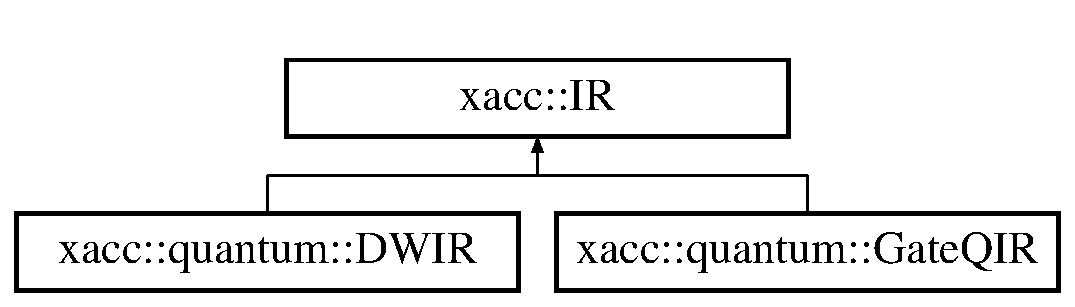
\includegraphics[height=2.000000cm]{a00050}
\end{center}
\end{figure}
\subsection*{Public Member Functions}
\begin{DoxyCompactItemize}
\item 
virtual std\+::string \hyperlink{a00050_a8356cdff1919b88eabeb84fd7450cdb6}{to\+Assembly\+String} (const std\+::string \&kernel\+Name, const std\+::string \&acc\+Buffer\+Var\+Name)=0
\item 
virtual void \hyperlink{a00050_a414b72224d88473ad6190bb88102a3ea}{persist} (std\+::ostream \&out\+Stream)=0
\item 
virtual void \hyperlink{a00050_a444c2e4dc0faac500fb70fa93997e9bc}{load} (std\+::istream \&in\+Stream)=0
\item 
virtual void \hyperlink{a00050_abbbf8e6993c518597de32cd05d49d737}{add\+Kernel} (std\+::shared\+\_\+ptr$<$ \hyperlink{a00038}{Function} $>$ kernel)=0
\item 
virtual bool \hyperlink{a00050_afc9ccf5126f3fed19c2e879133b2f6d8}{kernel\+Exists} (const std\+::string \&name)=0
\item 
virtual std\+::shared\+\_\+ptr$<$ \hyperlink{a00038}{Function} $>$ \hyperlink{a00050_a6f49b4ba4b3a15142b04873284885f0d}{get\+Kernel} (const std\+::string \&name)=0
\item 
virtual std\+::vector$<$ std\+::shared\+\_\+ptr$<$ \hyperlink{a00038}{Function} $>$ $>$ \hyperlink{a00050_a88c50bfc5b279145360ddc0c3a703b9b}{get\+Kernels} ()=0
\item 
virtual \hyperlink{a00050_a09a76d71092254acae07e19fa2f34921}{$\sim$\+IR} ()
\end{DoxyCompactItemize}


\subsection{Detailed Description}
The \hyperlink{a00050}{IR} interface is the base interface for derived accelerator-\/specific intermediate representations. At this level, an intermediate representation can be persisted to an assembly-\/like string, can be read in from file, and can be persisted to file. Since all X\+A\+CC intermediate representations operate on an \hyperlink{a00011}{Accelerator} Buffer, the \hyperlink{a00050}{IR} interface also provides a setter for such a buffer. 

\subsection{Constructor \& Destructor Documentation}
\index{xacc\+::\+IR@{xacc\+::\+IR}!````~IR@{$\sim$\+IR}}
\index{````~IR@{$\sim$\+IR}!xacc\+::\+IR@{xacc\+::\+IR}}
\subsubsection[{\texorpdfstring{$\sim$\+I\+R()}{~IR()}}]{\setlength{\rightskip}{0pt plus 5cm}virtual xacc\+::\+I\+R\+::$\sim$\+IR (
\begin{DoxyParamCaption}
{}
\end{DoxyParamCaption}
)\hspace{0.3cm}{\ttfamily [inline]}, {\ttfamily [virtual]}}\hypertarget{a00050_a09a76d71092254acae07e19fa2f34921}{}\label{a00050_a09a76d71092254acae07e19fa2f34921}
The destructor 

\subsection{Member Function Documentation}
\index{xacc\+::\+IR@{xacc\+::\+IR}!add\+Kernel@{add\+Kernel}}
\index{add\+Kernel@{add\+Kernel}!xacc\+::\+IR@{xacc\+::\+IR}}
\subsubsection[{\texorpdfstring{add\+Kernel(std\+::shared\+\_\+ptr$<$ Function $>$ kernel)=0}{addKernel(std::shared\_ptr< Function > kernel)=0}}]{\setlength{\rightskip}{0pt plus 5cm}virtual void xacc\+::\+I\+R\+::add\+Kernel (
\begin{DoxyParamCaption}
\item[{std\+::shared\+\_\+ptr$<$ {\bf Function} $>$}]{kernel}
\end{DoxyParamCaption}
)\hspace{0.3cm}{\ttfamily [pure virtual]}}\hypertarget{a00050_abbbf8e6993c518597de32cd05d49d737}{}\label{a00050_abbbf8e6993c518597de32cd05d49d737}
Add a new kernel to this \hyperlink{a00050}{IR} instance.


\begin{DoxyParams}{Parameters}
{\em kernel} & The \hyperlink{a00038}{Function} instance to add as a new kernel \\
\hline
\end{DoxyParams}


Implemented in \hyperlink{a00042_aa6ed2cf2cbcfec8105c327a4fa95346f}{xacc\+::quantum\+::\+Gate\+Q\+IR}, and \hyperlink{a00031_af1bef18e1e9568d1313b03149aab8c1b}{xacc\+::quantum\+::\+D\+W\+IR}.

\index{xacc\+::\+IR@{xacc\+::\+IR}!get\+Kernel@{get\+Kernel}}
\index{get\+Kernel@{get\+Kernel}!xacc\+::\+IR@{xacc\+::\+IR}}
\subsubsection[{\texorpdfstring{get\+Kernel(const std\+::string \&name)=0}{getKernel(const std::string \&name)=0}}]{\setlength{\rightskip}{0pt plus 5cm}virtual std\+::shared\+\_\+ptr$<${\bf Function}$>$ xacc\+::\+I\+R\+::get\+Kernel (
\begin{DoxyParamCaption}
\item[{const std\+::string \&}]{name}
\end{DoxyParamCaption}
)\hspace{0.3cm}{\ttfamily [pure virtual]}}\hypertarget{a00050_a6f49b4ba4b3a15142b04873284885f0d}{}\label{a00050_a6f49b4ba4b3a15142b04873284885f0d}
Return the kernel with the given name.


\begin{DoxyParams}{Parameters}
{\em name} & The name of the kernel to return. \\
\hline
\end{DoxyParams}
\begin{DoxyReturn}{Returns}
kernel The kernel with given name. 
\end{DoxyReturn}


Implemented in \hyperlink{a00042_a194758b6edcc3ae0c7fe8004f9bfe690}{xacc\+::quantum\+::\+Gate\+Q\+IR}, and \hyperlink{a00031_a38d8bdd24250749bc38ad31f8512fcfc}{xacc\+::quantum\+::\+D\+W\+IR}.

\index{xacc\+::\+IR@{xacc\+::\+IR}!get\+Kernels@{get\+Kernels}}
\index{get\+Kernels@{get\+Kernels}!xacc\+::\+IR@{xacc\+::\+IR}}
\subsubsection[{\texorpdfstring{get\+Kernels()=0}{getKernels()=0}}]{\setlength{\rightskip}{0pt plus 5cm}virtual std\+::vector$<$std\+::shared\+\_\+ptr$<${\bf Function}$>$ $>$ xacc\+::\+I\+R\+::get\+Kernels (
\begin{DoxyParamCaption}
{}
\end{DoxyParamCaption}
)\hspace{0.3cm}{\ttfamily [pure virtual]}}\hypertarget{a00050_a88c50bfc5b279145360ddc0c3a703b9b}{}\label{a00050_a88c50bfc5b279145360ddc0c3a703b9b}
Return all of this \hyperlink{a00050}{IR} instance\textquotesingle{}s kernels.

\begin{DoxyReturn}{Returns}
kernels The kernels this \hyperlink{a00050}{IR} contains. 
\end{DoxyReturn}


Implemented in \hyperlink{a00042_a4ace7ee5ebef84b1f39aaf5ed12c6cc6}{xacc\+::quantum\+::\+Gate\+Q\+IR}, and \hyperlink{a00031_a66e22c5dc95ec46045476864012ad08f}{xacc\+::quantum\+::\+D\+W\+IR}.

\index{xacc\+::\+IR@{xacc\+::\+IR}!kernel\+Exists@{kernel\+Exists}}
\index{kernel\+Exists@{kernel\+Exists}!xacc\+::\+IR@{xacc\+::\+IR}}
\subsubsection[{\texorpdfstring{kernel\+Exists(const std\+::string \&name)=0}{kernelExists(const std::string \&name)=0}}]{\setlength{\rightskip}{0pt plus 5cm}virtual bool xacc\+::\+I\+R\+::kernel\+Exists (
\begin{DoxyParamCaption}
\item[{const std\+::string \&}]{name}
\end{DoxyParamCaption}
)\hspace{0.3cm}{\ttfamily [pure virtual]}}\hypertarget{a00050_afc9ccf5126f3fed19c2e879133b2f6d8}{}\label{a00050_afc9ccf5126f3fed19c2e879133b2f6d8}
Return true if the kernel with given name exists in this \hyperlink{a00050}{IR}.


\begin{DoxyParams}{Parameters}
{\em name} & The name of the kernel to return. \\
\hline
\end{DoxyParams}
\begin{DoxyReturn}{Returns}
exists True if kernel exists. 
\end{DoxyReturn}


Implemented in \hyperlink{a00042_a692f95099caa7c024110a3f035941dca}{xacc\+::quantum\+::\+Gate\+Q\+IR}, and \hyperlink{a00031_ab5e8861d3bc0845bb015af6208f5f396}{xacc\+::quantum\+::\+D\+W\+IR}.

\index{xacc\+::\+IR@{xacc\+::\+IR}!load@{load}}
\index{load@{load}!xacc\+::\+IR@{xacc\+::\+IR}}
\subsubsection[{\texorpdfstring{load(std\+::istream \&in\+Stream)=0}{load(std::istream \&inStream)=0}}]{\setlength{\rightskip}{0pt plus 5cm}virtual void xacc\+::\+I\+R\+::load (
\begin{DoxyParamCaption}
\item[{std\+::istream \&}]{in\+Stream}
\end{DoxyParamCaption}
)\hspace{0.3cm}{\ttfamily [pure virtual]}}\hypertarget{a00050_a444c2e4dc0faac500fb70fa93997e9bc}{}\label{a00050_a444c2e4dc0faac500fb70fa93997e9bc}
Create this \hyperlink{a00050}{IR} instance from the given input stream.


\begin{DoxyParams}{Parameters}
{\em in\+Stream} & The input stream to read from. \\
\hline
\end{DoxyParams}


Implemented in \hyperlink{a00042_a07f26eeb362ac480d20da6cdc8c8fb39}{xacc\+::quantum\+::\+Gate\+Q\+IR}, and \hyperlink{a00031_a8b388d719d565bb902c979807d3d0d47}{xacc\+::quantum\+::\+D\+W\+IR}.

\index{xacc\+::\+IR@{xacc\+::\+IR}!persist@{persist}}
\index{persist@{persist}!xacc\+::\+IR@{xacc\+::\+IR}}
\subsubsection[{\texorpdfstring{persist(std\+::ostream \&out\+Stream)=0}{persist(std::ostream \&outStream)=0}}]{\setlength{\rightskip}{0pt plus 5cm}virtual void xacc\+::\+I\+R\+::persist (
\begin{DoxyParamCaption}
\item[{std\+::ostream \&}]{out\+Stream}
\end{DoxyParamCaption}
)\hspace{0.3cm}{\ttfamily [pure virtual]}}\hypertarget{a00050_a414b72224d88473ad6190bb88102a3ea}{}\label{a00050_a414b72224d88473ad6190bb88102a3ea}
Persist this \hyperlink{a00050}{IR} instance to the given output stream.


\begin{DoxyParams}{Parameters}
{\em out\+Stream} & The output stream to persist to. \\
\hline
\end{DoxyParams}


Implemented in \hyperlink{a00042_a40e1d07e4dfd3794ef53fca3cdbdca61}{xacc\+::quantum\+::\+Gate\+Q\+IR}, and \hyperlink{a00031_abcbfd0a4cf697843391c65cbd9a82080}{xacc\+::quantum\+::\+D\+W\+IR}.

\index{xacc\+::\+IR@{xacc\+::\+IR}!to\+Assembly\+String@{to\+Assembly\+String}}
\index{to\+Assembly\+String@{to\+Assembly\+String}!xacc\+::\+IR@{xacc\+::\+IR}}
\subsubsection[{\texorpdfstring{to\+Assembly\+String(const std\+::string \&kernel\+Name, const std\+::string \&acc\+Buffer\+Var\+Name)=0}{toAssemblyString(const std::string \&kernelName, const std::string \&accBufferVarName)=0}}]{\setlength{\rightskip}{0pt plus 5cm}virtual std\+::string xacc\+::\+I\+R\+::to\+Assembly\+String (
\begin{DoxyParamCaption}
\item[{const std\+::string \&}]{kernel\+Name, }
\item[{const std\+::string \&}]{acc\+Buffer\+Var\+Name}
\end{DoxyParamCaption}
)\hspace{0.3cm}{\ttfamily [pure virtual]}}\hypertarget{a00050_a8356cdff1919b88eabeb84fd7450cdb6}{}\label{a00050_a8356cdff1919b88eabeb84fd7450cdb6}
Return a assembly-\/like string representation of this intermediate representation


\begin{DoxyParams}{Parameters}
{\em kernel\+Name} & The name of hte kernel to persist to string \\
\hline
{\em acc\+Buffer\+Var\+Name} & The name of the \hyperlink{a00013}{Accelerator\+Buffer} \\
\hline
\end{DoxyParams}
\begin{DoxyReturn}{Returns}

\end{DoxyReturn}


Implemented in \hyperlink{a00042_a7153f7e9f516d43af3d5d4f95d60bd86}{xacc\+::quantum\+::\+Gate\+Q\+IR}, and \hyperlink{a00031_a880cb60197577ea31115331e3a030e3e}{xacc\+::quantum\+::\+D\+W\+IR}.



The documentation for this class was generated from the following file\+:\begin{DoxyCompactItemize}
\item 
I\+R.\+hpp\end{DoxyCompactItemize}

\hypertarget{a00051}{}\section{xacc\+:\+:I\+R\+Transformation Class Reference}
\label{a00051}\index{xacc\+::\+I\+R\+Transformation@{xacc\+::\+I\+R\+Transformation}}
\subsection*{Public Member Functions}
\begin{DoxyCompactItemize}
\item 
virtual void {\bfseries transform} (\hyperlink{a00050}{IR} \&ir)=0\hypertarget{a00051_accc69cba97f39aa3e51f81fec3ccf258}{}\label{a00051_accc69cba97f39aa3e51f81fec3ccf258}

\end{DoxyCompactItemize}


The documentation for this class was generated from the following file\+:\begin{DoxyCompactItemize}
\item 
I\+R\+Transformation.\+hpp\end{DoxyCompactItemize}

\hypertarget{a00052}{}\section{xacc\+:\+:quantum\+:\+:Json\+Visitor Class Reference}
\label{a00052}\index{xacc\+::quantum\+::\+Json\+Visitor@{xacc\+::quantum\+::\+Json\+Visitor}}


{\ttfamily \#include $<$Json\+Visitor.\+hpp$>$}

Inheritance diagram for xacc\+:\+:quantum\+:\+:Json\+Visitor\+:\begin{figure}[H]
\begin{center}
\leavevmode
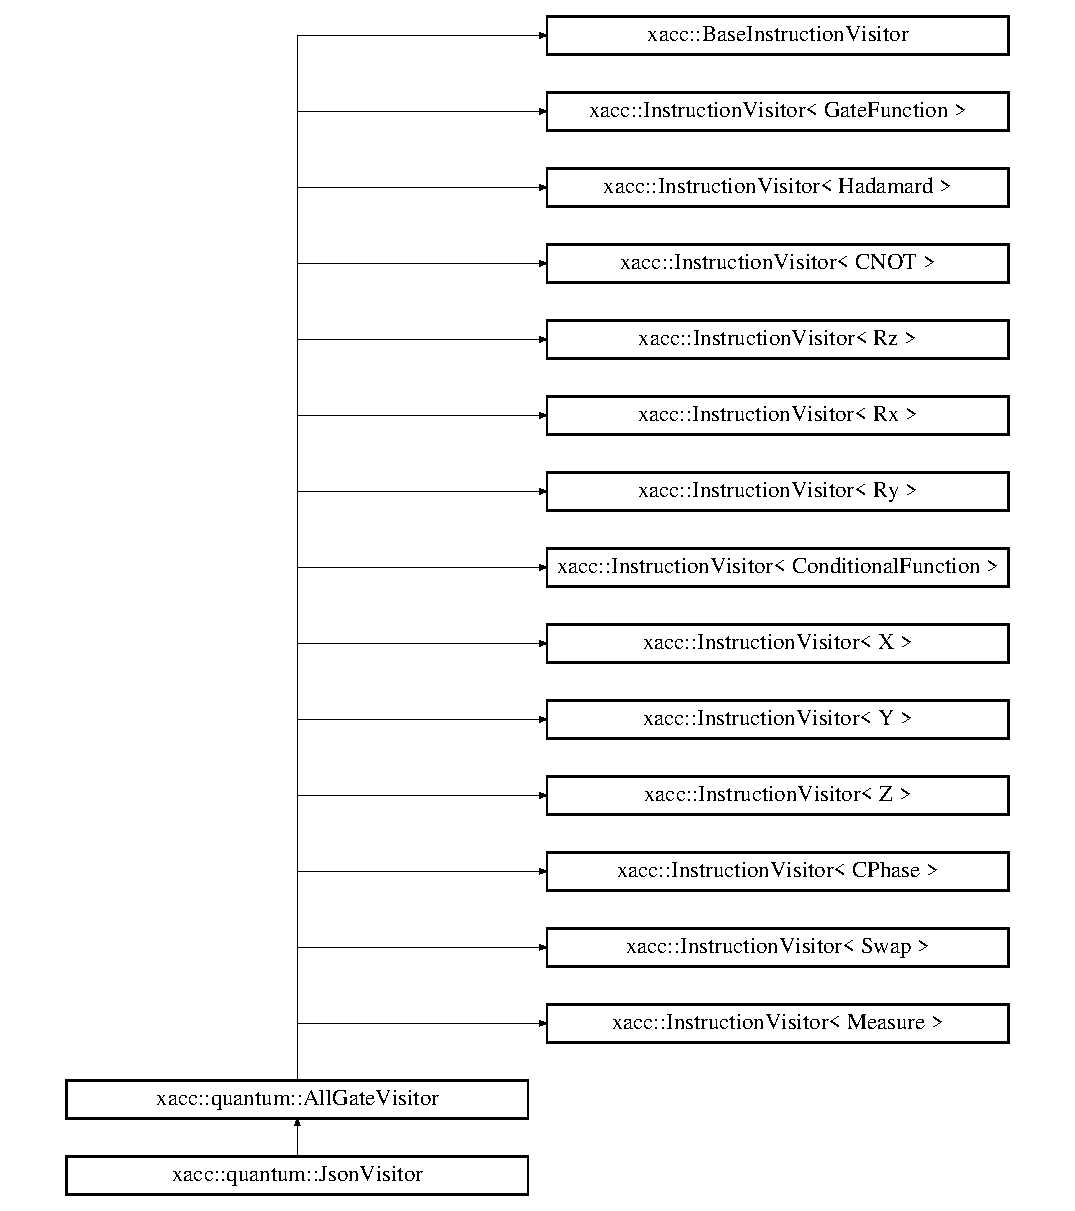
\includegraphics[height=12.000000cm]{a00052}
\end{center}
\end{figure}
\subsection*{Public Member Functions}
\begin{DoxyCompactItemize}
\item 
{\bfseries Json\+Visitor} (std\+::shared\+\_\+ptr$<$ \hyperlink{a00038}{xacc\+::\+Function} $>$ f)\hypertarget{a00052_a7b2bf70217828adf6457e3fee7e13056}{}\label{a00052_a7b2bf70217828adf6457e3fee7e13056}

\item 
{\bfseries Json\+Visitor} (std\+::vector$<$ std\+::shared\+\_\+ptr$<$ \hyperlink{a00038}{xacc\+::\+Function} $>$$>$ fs)\hypertarget{a00052_a7f2a81b621eaf97f3f7773b566320d02}{}\label{a00052_a7f2a81b621eaf97f3f7773b566320d02}

\item 
std\+::string {\bfseries write} ()\hypertarget{a00052_a78e2b6c71755a0fed97de43e0b7edc82}{}\label{a00052_a78e2b6c71755a0fed97de43e0b7edc82}

\item 
void {\bfseries visit} (\hyperlink{a00044}{Hadamard} \&h)\hypertarget{a00052_afdebbabdbae5ecb3a508f02ffe056fd4}{}\label{a00052_afdebbabdbae5ecb3a508f02ffe056fd4}

\item 
void {\bfseries visit} (\hyperlink{a00022}{C\+N\+OT} \&cn)\hypertarget{a00052_a83c17c122c0e02242189b3564290f3e9}{}\label{a00052_a83c17c122c0e02242189b3564290f3e9}

\item 
void {\bfseries visit} (\hyperlink{a00082}{Swap} \&s)\hypertarget{a00052_afd0b13a59603da5209f84f4b72f77a1a}{}\label{a00052_afd0b13a59603da5209f84f4b72f77a1a}

\item 
void {\bfseries visit} (\hyperlink{a00075}{Rz} \&rz)\hypertarget{a00052_a76c3593f3933631c2dbca74b7b216534}{}\label{a00052_a76c3593f3933631c2dbca74b7b216534}

\item 
void {\bfseries visit} (\hyperlink{a00073}{Rx} \&rx)\hypertarget{a00052_ad73ac1911e894f315fcee802673a30da}{}\label{a00052_ad73ac1911e894f315fcee802673a30da}

\item 
void {\bfseries visit} (\hyperlink{a00074}{Ry} \&ry)\hypertarget{a00052_a0e744d9db4c2d16196b17f91a84f8767}{}\label{a00052_a0e744d9db4c2d16196b17f91a84f8767}

\item 
void {\bfseries visit} (\hyperlink{a00027}{C\+Phase} \&cp)\hypertarget{a00052_aaac9aeecf38aa3e4dae4f43e3884b6d7}{}\label{a00052_aaac9aeecf38aa3e4dae4f43e3884b6d7}

\item 
void {\bfseries visit} (\hyperlink{a00025}{Conditional\+Function} \&cn)\hypertarget{a00052_aea63f829d8c926e567ef6a09a0ca779e}{}\label{a00052_aea63f829d8c926e567ef6a09a0ca779e}

\item 
void {\bfseries visit} (\hyperlink{a00055}{Measure} \&cn)\hypertarget{a00052_a71a9c4b78152af3366f8ee93b2e4d9da}{}\label{a00052_a71a9c4b78152af3366f8ee93b2e4d9da}

\item 
void {\bfseries visit} (\hyperlink{a00084}{X} \&cn)\hypertarget{a00052_a2862d01b12da46374c16a3baf33bb4ca}{}\label{a00052_a2862d01b12da46374c16a3baf33bb4ca}

\item 
void {\bfseries visit} (\hyperlink{a00087}{Y} \&y)\hypertarget{a00052_a5f08b133da5ae583b40d3324220e68e3}{}\label{a00052_a5f08b133da5ae583b40d3324220e68e3}

\item 
void {\bfseries visit} (\hyperlink{a00088}{Z} \&z)\hypertarget{a00052_a1e1a24feb419b275e2873575242ecbfd}{}\label{a00052_a1e1a24feb419b275e2873575242ecbfd}

\item 
void {\bfseries visit} (\hyperlink{a00040}{Gate\+Function} \&function)\hypertarget{a00052_af80f9bd5dda7f53279baa9823c715f60}{}\label{a00052_af80f9bd5dda7f53279baa9823c715f60}

\end{DoxyCompactItemize}
\subsection*{Protected Member Functions}
\begin{DoxyCompactItemize}
\item 
void {\bfseries base\+Gate\+Inst} (\hyperlink{a00041}{Gate\+Instruction} \&inst, bool end\+Object=true)\hypertarget{a00052_adf4795f80bf4773af8babb9ee7d38c96}{}\label{a00052_adf4795f80bf4773af8babb9ee7d38c96}

\end{DoxyCompactItemize}
\subsection*{Protected Attributes}
\begin{DoxyCompactItemize}
\item 
std\+::shared\+\_\+ptr$<$ String\+Buffer $>$ {\bfseries buffer}\hypertarget{a00052_a79e14ac35a004c64f3b6a5c684d73598}{}\label{a00052_a79e14ac35a004c64f3b6a5c684d73598}

\item 
std\+::shared\+\_\+ptr$<$ Writer $>$ {\bfseries writer}\hypertarget{a00052_a4433a92e0c5a1ede71223c275a495241}{}\label{a00052_a4433a92e0c5a1ede71223c275a495241}

\item 
std\+::shared\+\_\+ptr$<$ \hyperlink{a00038}{Function} $>$ {\bfseries function}\hypertarget{a00052_ae943110fac6aa057637fbdf76c39ba9c}{}\label{a00052_ae943110fac6aa057637fbdf76c39ba9c}

\item 
std\+::shared\+\_\+ptr$<$ \hyperlink{a00047}{Instruction\+Iterator} $>$ {\bfseries top\+Level\+Instruction\+Iterator}\hypertarget{a00052_a84ac738710890faa124c0df935bc51d5}{}\label{a00052_a84ac738710890faa124c0df935bc51d5}

\item 
std\+::vector$<$ std\+::shared\+\_\+ptr$<$ \hyperlink{a00038}{Function} $>$ $>$ {\bfseries functions}\hypertarget{a00052_a3f883a147fed57e8b241a2700f4602d9}{}\label{a00052_a3f883a147fed57e8b241a2700f4602d9}

\end{DoxyCompactItemize}


\subsection{Detailed Description}
F\+I\+X\+ME write this 

The documentation for this class was generated from the following file\+:\begin{DoxyCompactItemize}
\item 
Json\+Visitor.\+hpp\end{DoxyCompactItemize}

\hypertarget{a00053}{}\section{xacc\+:\+:quantum\+:\+:K44\+Bipartite Class Reference}
\label{a00053}\index{xacc\+::quantum\+::\+K44\+Bipartite@{xacc\+::quantum\+::\+K44\+Bipartite}}
Inheritance diagram for xacc\+:\+:quantum\+:\+:K44\+Bipartite\+:\begin{figure}[H]
\begin{center}
\leavevmode
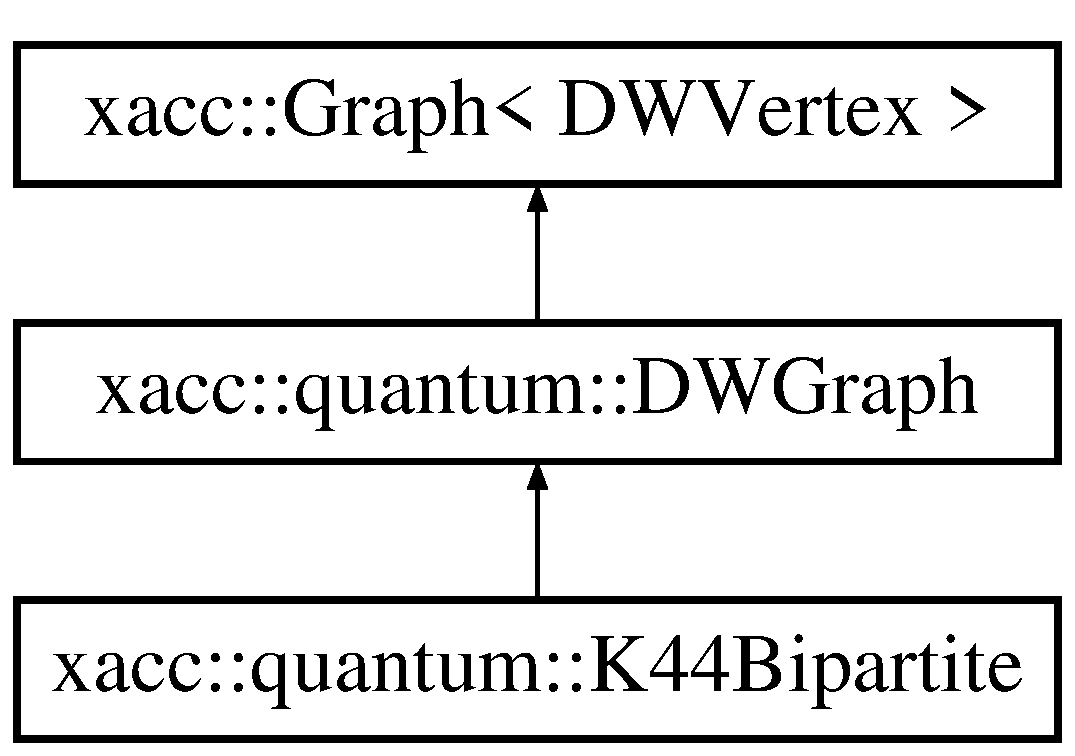
\includegraphics[height=3.000000cm]{a00053}
\end{center}
\end{figure}
\subsection*{Additional Inherited Members}


The documentation for this class was generated from the following file\+:\begin{DoxyCompactItemize}
\item 
D\+W\+Graph.\+hpp\end{DoxyCompactItemize}

\hypertarget{a00054}{}\section{xacc\+:\+:quantum\+:\+:Kernel\+Replacement\+Preprocessor Class Reference}
\label{a00054}\index{xacc\+::quantum\+::\+Kernel\+Replacement\+Preprocessor@{xacc\+::quantum\+::\+Kernel\+Replacement\+Preprocessor}}


{\ttfamily \#include $<$Kernel\+Replacement\+Preprocessor.\+hpp$>$}

Inheritance diagram for xacc\+:\+:quantum\+:\+:Kernel\+Replacement\+Preprocessor\+:\begin{figure}[H]
\begin{center}
\leavevmode
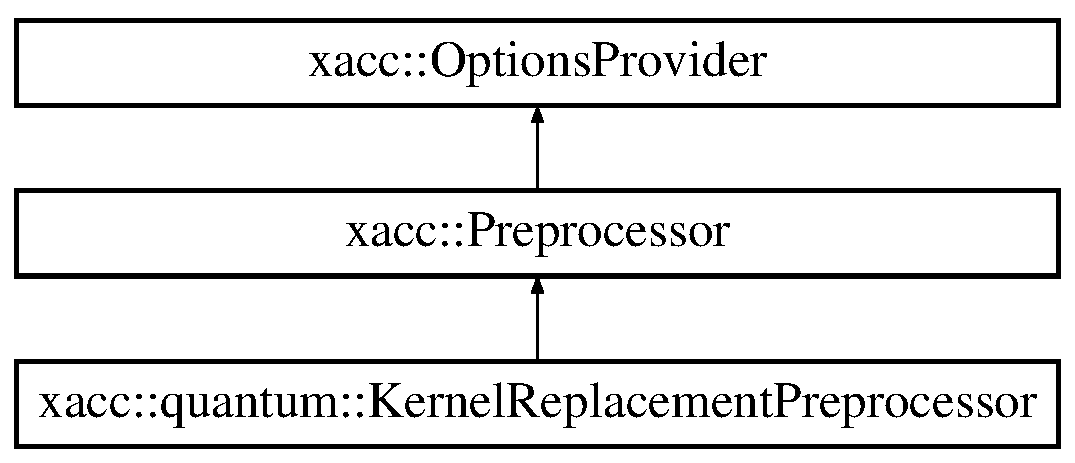
\includegraphics[height=3.000000cm]{a00054}
\end{center}
\end{figure}
\subsection*{Public Member Functions}
\begin{DoxyCompactItemize}
\item 
virtual const std\+::string \hyperlink{a00054_ad4f9ba1f83ea45ed376f36e3853c668d}{process} (const std\+::string \&source, std\+::shared\+\_\+ptr$<$ \hyperlink{a00023}{Compiler} $>$ compiler, std\+::shared\+\_\+ptr$<$ \hyperlink{a00011}{Accelerator} $>$ accelerator)
\item 
virtual const std\+::string \hyperlink{a00054_af74db6b7f3adeb7d203777f5ce450491}{get\+Name} ()
\end{DoxyCompactItemize}


\subsection{Detailed Description}
The \hyperlink{a00054}{Kernel\+Replacement\+Preprocessor} is a preprocessor for gate model quantum computing that analyzing quantum kernel source code and looks for occurrences of \textquotesingle{}xacc\+::\+F\+U\+N\+C\+T\+I\+ON\textquotesingle{} strings (for example, xacc\+::\+Q\+F\+T(qreg)).

Once one of these occurrences is found, this preprocessor queries the \hyperlink{a00014}{Algorithm\+Generator} \hyperlink{a00070}{Registry} for any available Algorithm\+Generators with that name. If such an \hyperlink{a00014}{Algorithm\+Generator} exists, it generates the X\+A\+CC \hyperlink{a00050}{IR} instance for that algorithm, translates the \hyperlink{a00050}{IR} to the \hyperlink{a00023}{Compiler}\textquotesingle{}s source code representation, and replaces the \textquotesingle{}xacc\+::\+F\+U\+N\+C\+T\+I\+ON\textquotesingle{} occurrence with the new source code. 

\subsection{Member Function Documentation}
\index{xacc\+::quantum\+::\+Kernel\+Replacement\+Preprocessor@{xacc\+::quantum\+::\+Kernel\+Replacement\+Preprocessor}!get\+Name@{get\+Name}}
\index{get\+Name@{get\+Name}!xacc\+::quantum\+::\+Kernel\+Replacement\+Preprocessor@{xacc\+::quantum\+::\+Kernel\+Replacement\+Preprocessor}}
\subsubsection[{\texorpdfstring{get\+Name()}{getName()}}]{\setlength{\rightskip}{0pt plus 5cm}virtual const std\+::string xacc\+::quantum\+::\+Kernel\+Replacement\+Preprocessor\+::get\+Name (
\begin{DoxyParamCaption}
{}
\end{DoxyParamCaption}
)\hspace{0.3cm}{\ttfamily [inline]}, {\ttfamily [virtual]}}\hypertarget{a00054_af74db6b7f3adeb7d203777f5ce450491}{}\label{a00054_af74db6b7f3adeb7d203777f5ce450491}
Return the name of this \hyperlink{a00057}{Preprocessor} \begin{DoxyReturn}{Returns}
name \hyperlink{a00057}{Preprocessor} name 
\end{DoxyReturn}


Implements \hyperlink{a00057_a36671f4c062d61e230306edc404774cd}{xacc\+::\+Preprocessor}.

\index{xacc\+::quantum\+::\+Kernel\+Replacement\+Preprocessor@{xacc\+::quantum\+::\+Kernel\+Replacement\+Preprocessor}!process@{process}}
\index{process@{process}!xacc\+::quantum\+::\+Kernel\+Replacement\+Preprocessor@{xacc\+::quantum\+::\+Kernel\+Replacement\+Preprocessor}}
\subsubsection[{\texorpdfstring{process(const std\+::string \&source, std\+::shared\+\_\+ptr$<$ Compiler $>$ compiler, std\+::shared\+\_\+ptr$<$ Accelerator $>$ accelerator)}{process(const std::string \&source, std::shared\_ptr< Compiler > compiler, std::shared\_ptr< Accelerator > accelerator)}}]{\setlength{\rightskip}{0pt plus 5cm}const std\+::string xacc\+::quantum\+::\+Kernel\+Replacement\+Preprocessor\+::process (
\begin{DoxyParamCaption}
\item[{const std\+::string \&}]{source, }
\item[{std\+::shared\+\_\+ptr$<$ {\bf Compiler} $>$}]{compiler, }
\item[{std\+::shared\+\_\+ptr$<$ {\bf Accelerator} $>$}]{accelerator}
\end{DoxyParamCaption}
)\hspace{0.3cm}{\ttfamily [virtual]}}\hypertarget{a00054_ad4f9ba1f83ea45ed376f36e3853c668d}{}\label{a00054_ad4f9ba1f83ea45ed376f36e3853c668d}
This method replaces xacc\+::\+F\+U\+N\+C\+T\+I\+ON references with actual Compiler-\/specific source code.


\begin{DoxyParams}{Parameters}
{\em src} & The unprocessed kernel source code \\
\hline
{\em compiler} & The compiler being used to compile the code \\
\hline
{\em accelerator} & The \hyperlink{a00011}{Accelerator} this code will be run on\\
\hline
\end{DoxyParams}
\begin{DoxyReturn}{Returns}
processed\+Src The processed kernel source code 
\end{DoxyReturn}


Implements \hyperlink{a00057_ae59b5a2963f8bcc84b590a83f4749e19}{xacc\+::\+Preprocessor}.



The documentation for this class was generated from the following files\+:\begin{DoxyCompactItemize}
\item 
Kernel\+Replacement\+Preprocessor.\+hpp\item 
Kernel\+Replacement\+Preprocessor.\+cpp\end{DoxyCompactItemize}

\hypertarget{a00055}{}\section{xacc\+:\+:quantum\+:\+:Measure Class Reference}
\label{a00055}\index{xacc\+::quantum\+::\+Measure@{xacc\+::quantum\+::\+Measure}}
Inheritance diagram for xacc\+:\+:quantum\+:\+:Measure\+:\begin{figure}[H]
\begin{center}
\leavevmode
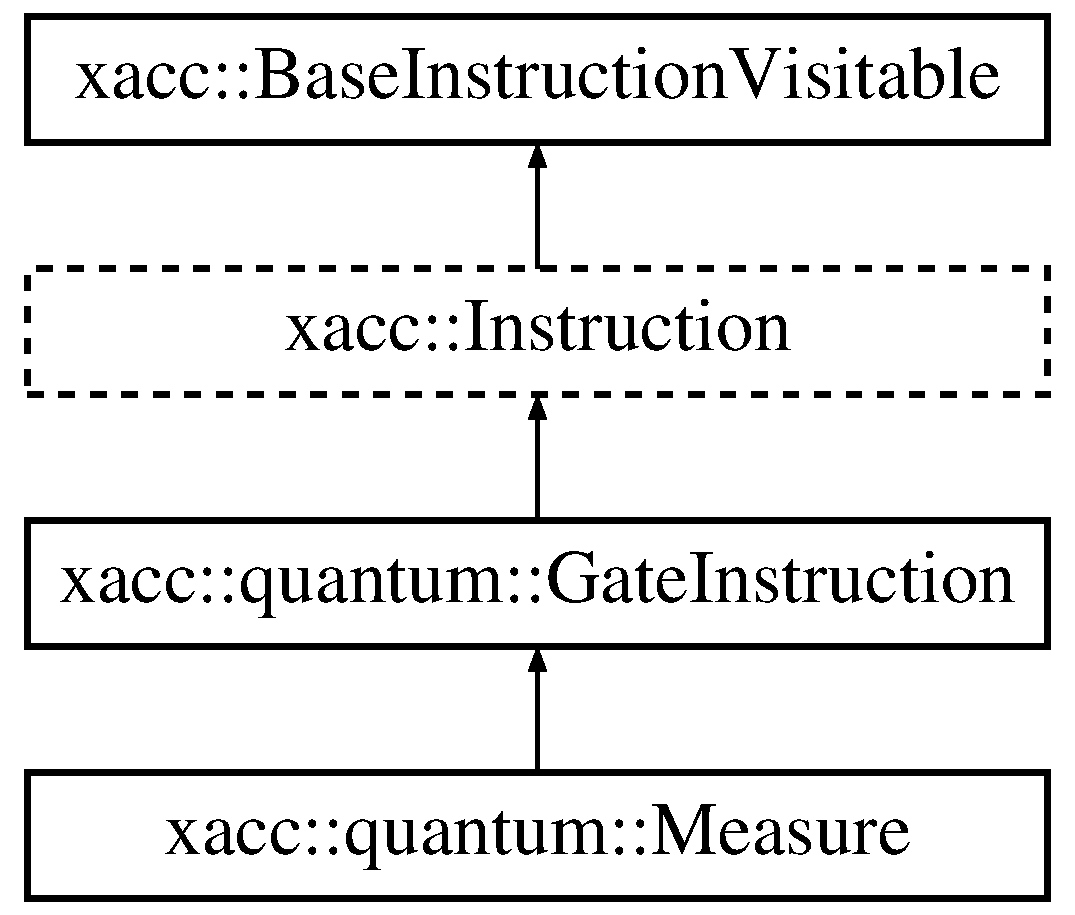
\includegraphics[height=4.000000cm]{a00055}
\end{center}
\end{figure}
\subsection*{Public Member Functions}
\begin{DoxyCompactItemize}
\item 
{\bfseries Measure} (std\+::vector$<$ int $>$ qbit)\hypertarget{a00055_afe330a0eea029d842ff9c88a817dcc7d}{}\label{a00055_afe330a0eea029d842ff9c88a817dcc7d}

\item 
{\bfseries Measure} (int qbit, int classical\+Idx)\hypertarget{a00055_a9b8d9edca8ad2c3fb132780200f17335}{}\label{a00055_a9b8d9edca8ad2c3fb132780200f17335}

\item 
virtual const std\+::string \hyperlink{a00055_a1c51a5d68294dcb2ba1a9fbea63a730f}{to\+String} (const std\+::string \&buffer\+Var\+Name)
\item 
int {\bfseries get\+Classical\+Bit\+Index} ()\hypertarget{a00055_a0cb3c94731544042807236ade36fddd0}{}\label{a00055_a0cb3c94731544042807236ade36fddd0}

\end{DoxyCompactItemize}
\subsection*{Additional Inherited Members}


\subsection{Member Function Documentation}
\index{xacc\+::quantum\+::\+Measure@{xacc\+::quantum\+::\+Measure}!to\+String@{to\+String}}
\index{to\+String@{to\+String}!xacc\+::quantum\+::\+Measure@{xacc\+::quantum\+::\+Measure}}
\subsubsection[{\texorpdfstring{to\+String(const std\+::string \&buffer\+Var\+Name)}{toString(const std::string \&bufferVarName)}}]{\setlength{\rightskip}{0pt plus 5cm}const std\+::string xacc\+::quantum\+::\+Measure\+::to\+String (
\begin{DoxyParamCaption}
\item[{const std\+::string \&}]{buffer\+Var\+Name}
\end{DoxyParamCaption}
)\hspace{0.3cm}{\ttfamily [virtual]}}\hypertarget{a00055_a1c51a5d68294dcb2ba1a9fbea63a730f}{}\label{a00055_a1c51a5d68294dcb2ba1a9fbea63a730f}
Return this instruction\textquotesingle{}s assembly-\/like string representation. 
\begin{DoxyParams}{Parameters}
{\em buffer\+Var\+Name} & \\
\hline
\end{DoxyParams}
\begin{DoxyReturn}{Returns}

\end{DoxyReturn}


Reimplemented from \hyperlink{a00041_a089a5da67ff40ac1a6f56e64589822d9}{xacc\+::quantum\+::\+Gate\+Instruction}.



The documentation for this class was generated from the following files\+:\begin{DoxyCompactItemize}
\item 
Measure.\+hpp\item 
Measure.\+cpp\end{DoxyCompactItemize}

\hypertarget{a00056}{}\section{xacc\+:\+:Options\+Provider Class Reference}
\label{a00056}\index{xacc\+::\+Options\+Provider@{xacc\+::\+Options\+Provider}}


{\ttfamily \#include $<$Options\+Provider.\+hpp$>$}

Inheritance diagram for xacc\+:\+:Options\+Provider\+:\begin{figure}[H]
\begin{center}
\leavevmode
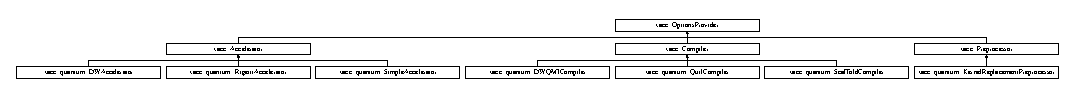
\includegraphics[height=0.824742cm]{a00056}
\end{center}
\end{figure}
\subsection*{Public Member Functions}
\begin{DoxyCompactItemize}
\item 
virtual std\+::shared\+\_\+ptr$<$ options\+\_\+description $>$ \hyperlink{a00056_a6d150954f852109bfe2c1ae90222926f}{get\+Options} ()=0
\item 
virtual \hyperlink{a00056_a7782757b419792ff346f563517eed8b8}{$\sim$\+Options\+Provider} ()
\end{DoxyCompactItemize}


\subsection{Detailed Description}
The \hyperlink{a00056}{Options\+Provider} interface enables derived subclasses to provide a description of any and all command line options that they can take to drive and control their execution and behavior. 

\subsection{Constructor \& Destructor Documentation}
\index{xacc\+::\+Options\+Provider@{xacc\+::\+Options\+Provider}!````~Options\+Provider@{$\sim$\+Options\+Provider}}
\index{````~Options\+Provider@{$\sim$\+Options\+Provider}!xacc\+::\+Options\+Provider@{xacc\+::\+Options\+Provider}}
\subsubsection[{\texorpdfstring{$\sim$\+Options\+Provider()}{~OptionsProvider()}}]{\setlength{\rightskip}{0pt plus 5cm}virtual xacc\+::\+Options\+Provider\+::$\sim$\+Options\+Provider (
\begin{DoxyParamCaption}
{}
\end{DoxyParamCaption}
)\hspace{0.3cm}{\ttfamily [inline]}, {\ttfamily [virtual]}}\hypertarget{a00056_a7782757b419792ff346f563517eed8b8}{}\label{a00056_a7782757b419792ff346f563517eed8b8}
The destructor 

\subsection{Member Function Documentation}
\index{xacc\+::\+Options\+Provider@{xacc\+::\+Options\+Provider}!get\+Options@{get\+Options}}
\index{get\+Options@{get\+Options}!xacc\+::\+Options\+Provider@{xacc\+::\+Options\+Provider}}
\subsubsection[{\texorpdfstring{get\+Options()=0}{getOptions()=0}}]{\setlength{\rightskip}{0pt plus 5cm}virtual std\+::shared\+\_\+ptr$<$options\+\_\+description$>$ xacc\+::\+Options\+Provider\+::get\+Options (
\begin{DoxyParamCaption}
{}
\end{DoxyParamCaption}
)\hspace{0.3cm}{\ttfamily [pure virtual]}}\hypertarget{a00056_a6d150954f852109bfe2c1ae90222926f}{}\label{a00056_a6d150954f852109bfe2c1ae90222926f}
Return a Boost options\+\_\+description instance that describes the options available for this derived subclass. 

Implemented in \hyperlink{a00011_a98c9eda6b54367c75667ecfbbf167979}{xacc\+::\+Accelerator}, \hyperlink{a00029_a09926db9f99706307ae6ce5b56845bca}{xacc\+::quantum\+::\+D\+W\+Accelerator}, \hyperlink{a00071_a9ee9e62aecbccf193894ca3388676f9f}{xacc\+::quantum\+::\+Rigetti\+Accelerator}, \hyperlink{a00023_a9f5a8965c9c2dd895016d18264ebbe92}{xacc\+::\+Compiler}, \hyperlink{a00034_a0851334cc33b5b1da2694150a0a1a43c}{xacc\+::quantum\+::\+D\+W\+Q\+M\+I\+Compiler}, and \hyperlink{a00057_a96f5600ea47628b66917c7b90250e7f1}{xacc\+::\+Preprocessor}.



The documentation for this class was generated from the following file\+:\begin{DoxyCompactItemize}
\item 
Options\+Provider.\+hpp\end{DoxyCompactItemize}

\hypertarget{a00057}{}\section{xacc\+:\+:Preprocessor Class Reference}
\label{a00057}\index{xacc\+::\+Preprocessor@{xacc\+::\+Preprocessor}}


{\ttfamily \#include $<$Preprocessor.\+hpp$>$}

Inheritance diagram for xacc\+:\+:Preprocessor\+:\begin{figure}[H]
\begin{center}
\leavevmode
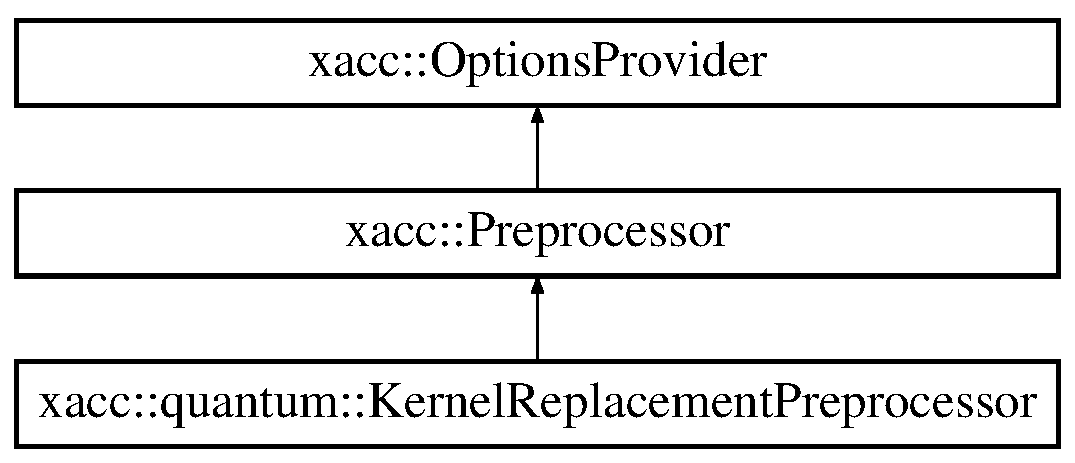
\includegraphics[height=3.000000cm]{a00057}
\end{center}
\end{figure}
\subsection*{Public Member Functions}
\begin{DoxyCompactItemize}
\item 
virtual const std\+::string \hyperlink{a00057_ae59b5a2963f8bcc84b590a83f4749e19}{process} (const std\+::string \&source, std\+::shared\+\_\+ptr$<$ \hyperlink{a00023}{Compiler} $>$ compiler, std\+::shared\+\_\+ptr$<$ \hyperlink{a00011}{Accelerator} $>$ accelerator)=0
\item 
virtual const std\+::string \hyperlink{a00057_a36671f4c062d61e230306edc404774cd}{get\+Name} ()=0
\item 
virtual std\+::shared\+\_\+ptr$<$ options\+\_\+description $>$ \hyperlink{a00057_a96f5600ea47628b66917c7b90250e7f1}{get\+Options} ()
\end{DoxyCompactItemize}


\subsection{Detailed Description}
The \hyperlink{a00057}{Preprocessor} interface provides a mechanism for processing quantum kernel source code before compilation takes place. Realizations of this interface implement the process method which takes as input the source code to process, and the compiler and accelerator this code is targeted at. 

\subsection{Member Function Documentation}
\index{xacc\+::\+Preprocessor@{xacc\+::\+Preprocessor}!get\+Name@{get\+Name}}
\index{get\+Name@{get\+Name}!xacc\+::\+Preprocessor@{xacc\+::\+Preprocessor}}
\subsubsection[{\texorpdfstring{get\+Name()=0}{getName()=0}}]{\setlength{\rightskip}{0pt plus 5cm}virtual const std\+::string xacc\+::\+Preprocessor\+::get\+Name (
\begin{DoxyParamCaption}
{}
\end{DoxyParamCaption}
)\hspace{0.3cm}{\ttfamily [pure virtual]}}\hypertarget{a00057_a36671f4c062d61e230306edc404774cd}{}\label{a00057_a36671f4c062d61e230306edc404774cd}
Return the name of this \hyperlink{a00057}{Preprocessor}

\begin{DoxyReturn}{Returns}
name The name of this preprocessor 
\end{DoxyReturn}


Implemented in \hyperlink{a00054_af74db6b7f3adeb7d203777f5ce450491}{xacc\+::quantum\+::\+Kernel\+Replacement\+Preprocessor}.

\index{xacc\+::\+Preprocessor@{xacc\+::\+Preprocessor}!get\+Options@{get\+Options}}
\index{get\+Options@{get\+Options}!xacc\+::\+Preprocessor@{xacc\+::\+Preprocessor}}
\subsubsection[{\texorpdfstring{get\+Options()}{getOptions()}}]{\setlength{\rightskip}{0pt plus 5cm}virtual std\+::shared\+\_\+ptr$<$options\+\_\+description$>$ xacc\+::\+Preprocessor\+::get\+Options (
\begin{DoxyParamCaption}
{}
\end{DoxyParamCaption}
)\hspace{0.3cm}{\ttfamily [inline]}, {\ttfamily [virtual]}}\hypertarget{a00057_a96f5600ea47628b66917c7b90250e7f1}{}\label{a00057_a96f5600ea47628b66917c7b90250e7f1}
Return an empty options\+\_\+description, this is for subclasses to implement. 

Implements \hyperlink{a00056_a6d150954f852109bfe2c1ae90222926f}{xacc\+::\+Options\+Provider}.

\index{xacc\+::\+Preprocessor@{xacc\+::\+Preprocessor}!process@{process}}
\index{process@{process}!xacc\+::\+Preprocessor@{xacc\+::\+Preprocessor}}
\subsubsection[{\texorpdfstring{process(const std\+::string \&source, std\+::shared\+\_\+ptr$<$ Compiler $>$ compiler, std\+::shared\+\_\+ptr$<$ Accelerator $>$ accelerator)=0}{process(const std::string \&source, std::shared\_ptr< Compiler > compiler, std::shared\_ptr< Accelerator > accelerator)=0}}]{\setlength{\rightskip}{0pt plus 5cm}virtual const std\+::string xacc\+::\+Preprocessor\+::process (
\begin{DoxyParamCaption}
\item[{const std\+::string \&}]{source, }
\item[{std\+::shared\+\_\+ptr$<$ {\bf Compiler} $>$}]{compiler, }
\item[{std\+::shared\+\_\+ptr$<$ {\bf Accelerator} $>$}]{accelerator}
\end{DoxyParamCaption}
)\hspace{0.3cm}{\ttfamily [pure virtual]}}\hypertarget{a00057_ae59b5a2963f8bcc84b590a83f4749e19}{}\label{a00057_ae59b5a2963f8bcc84b590a83f4749e19}
This method is to be implemented by subclasses to take in a kernel source string and process it in an isomorphic manner, and returns the processed source code.


\begin{DoxyParams}{Parameters}
{\em src} & The unprocessed kernel source code \\
\hline
{\em compiler} & The compiler being used to compile the code \\
\hline
{\em accelerator} & The \hyperlink{a00011}{Accelerator} this code will be run on\\
\hline
\end{DoxyParams}
\begin{DoxyReturn}{Returns}
processed\+Src The processed kernel source code 
\end{DoxyReturn}


Implemented in \hyperlink{a00054_ad4f9ba1f83ea45ed376f36e3853c668d}{xacc\+::quantum\+::\+Kernel\+Replacement\+Preprocessor}.



The documentation for this class was generated from the following file\+:\begin{DoxyCompactItemize}
\item 
Preprocessor.\+hpp\end{DoxyCompactItemize}

\hypertarget{a00058}{}\section{xacc\+:\+:Program Class Reference}
\label{a00058}\index{xacc\+::\+Program@{xacc\+::\+Program}}


{\ttfamily \#include $<$Program.\+hpp$>$}

\subsection*{Public Member Functions}
\begin{DoxyCompactItemize}
\item 
\hyperlink{a00058_a6d20079fde67a3ef145315e762249115}{Program} (std\+::shared\+\_\+ptr$<$ \hyperlink{a00011}{Accelerator} $>$ acc, const std\+::string \&source\+File)
\item 
{\footnotesize template$<$typename... Runtime\+Args$>$ }\\std\+::function$<$ void(std\+::shared\+\_\+ptr$<$ \hyperlink{a00013}{Accelerator\+Buffer} $>$, Runtime\+Args...)$>$ \hyperlink{a00058_abf5023c9f01cac8a506bdef86760e8f1}{get\+Kernel} (const std\+::string \&kernel\+Name)
\end{DoxyCompactItemize}
\subsection*{Protected Member Functions}
\begin{DoxyCompactItemize}
\item 
void \hyperlink{a00058_a53079c7886c0be065968bcf6674d1516}{build} ()
\end{DoxyCompactItemize}
\subsection*{Protected Attributes}
\begin{DoxyCompactItemize}
\item 
std\+::string \hyperlink{a00058_aae78160f9f9e52a3e0c9b342996a7202}{src}
\item 
std\+::shared\+\_\+ptr$<$ \hyperlink{a00011}{Accelerator} $>$ \hyperlink{a00058_a10c948629c84f23dd426c04a9a518155}{accelerator}
\item 
std\+::shared\+\_\+ptr$<$ \hyperlink{a00050}{IR} $>$ \hyperlink{a00058_a5681f0989fc1c3fced8e30e815d6511c}{xacc\+IR}
\item 
std\+::shared\+\_\+ptr$<$ \hyperlink{a00023}{Compiler} $>$ \hyperlink{a00058_a0d2ae2522bb0daad0eea7871fc4e2061}{compiler}
\end{DoxyCompactItemize}


\subsection{Detailed Description}
The \hyperlink{a00058}{Program} is the main entrypoint for the X\+A\+CC A\+PI. Users with accelerator kernels must construct a valid \hyperlink{a00058}{Program} to be compiled and executed on the attached accelerator. Programs must be given the \hyperlink{a00011}{Accelerator} reference to be used and kernel source code at construction time. 

\subsection{Constructor \& Destructor Documentation}
\index{xacc\+::\+Program@{xacc\+::\+Program}!Program@{Program}}
\index{Program@{Program}!xacc\+::\+Program@{xacc\+::\+Program}}
\subsubsection[{\texorpdfstring{Program(std\+::shared\+\_\+ptr$<$ Accelerator $>$ acc, const std\+::string \&source\+File)}{Program(std::shared\_ptr< Accelerator > acc, const std::string \&sourceFile)}}]{\setlength{\rightskip}{0pt plus 5cm}xacc\+::\+Program\+::\+Program (
\begin{DoxyParamCaption}
\item[{std\+::shared\+\_\+ptr$<$ {\bf Accelerator} $>$}]{acc, }
\item[{const std\+::string \&}]{source\+File}
\end{DoxyParamCaption}
)\hspace{0.3cm}{\ttfamily [inline]}}\hypertarget{a00058_a6d20079fde67a3ef145315e762249115}{}\label{a00058_a6d20079fde67a3ef145315e762249115}
The Constructor, takes the \hyperlink{a00011}{Accelerator} to execute on, and the source to compile and execute


\begin{DoxyParams}{Parameters}
{\em acc} & Attached \hyperlink{a00011}{Accelerator} to execute \\
\hline
{\em source\+File} & The kernel source code \\
\hline
\end{DoxyParams}


\subsection{Member Function Documentation}
\index{xacc\+::\+Program@{xacc\+::\+Program}!build@{build}}
\index{build@{build}!xacc\+::\+Program@{xacc\+::\+Program}}
\subsubsection[{\texorpdfstring{build()}{build()}}]{\setlength{\rightskip}{0pt plus 5cm}void xacc\+::\+Program\+::build (
\begin{DoxyParamCaption}
{}
\end{DoxyParamCaption}
)\hspace{0.3cm}{\ttfamily [inline]}, {\ttfamily [protected]}}\hypertarget{a00058_a53079c7886c0be065968bcf6674d1516}{}\label{a00058_a53079c7886c0be065968bcf6674d1516}
Execute the compilation mechanism on the provided program source kernel code to produce X\+A\+CC \hyperlink{a00050}{IR} that can be executed on the attached \hyperlink{a00011}{Accelerator}. \index{xacc\+::\+Program@{xacc\+::\+Program}!get\+Kernel@{get\+Kernel}}
\index{get\+Kernel@{get\+Kernel}!xacc\+::\+Program@{xacc\+::\+Program}}
\subsubsection[{\texorpdfstring{get\+Kernel(const std\+::string \&kernel\+Name)}{getKernel(const std::string \&kernelName)}}]{\setlength{\rightskip}{0pt plus 5cm}template$<$typename... Runtime\+Args$>$ std\+::function$<$void(std\+::shared\+\_\+ptr$<${\bf Accelerator\+Buffer}$>$, Runtime\+Args...)$>$ xacc\+::\+Program\+::get\+Kernel (
\begin{DoxyParamCaption}
\item[{const std\+::string \&}]{kernel\+Name}
\end{DoxyParamCaption}
)\hspace{0.3cm}{\ttfamily [inline]}}\hypertarget{a00058_abf5023c9f01cac8a506bdef86760e8f1}{}\label{a00058_abf5023c9f01cac8a506bdef86760e8f1}
Return an executable version of the quantum kernel referenced by the kernel\+Name string.


\begin{DoxyParams}{Parameters}
{\em name} & \\
\hline
{\em args} & \\
\hline
\end{DoxyParams}
\begin{DoxyReturn}{Returns}

\end{DoxyReturn}


\subsection{Member Data Documentation}
\index{xacc\+::\+Program@{xacc\+::\+Program}!accelerator@{accelerator}}
\index{accelerator@{accelerator}!xacc\+::\+Program@{xacc\+::\+Program}}
\subsubsection[{\texorpdfstring{accelerator}{accelerator}}]{\setlength{\rightskip}{0pt plus 5cm}std\+::shared\+\_\+ptr$<${\bf Accelerator}$>$ xacc\+::\+Program\+::accelerator\hspace{0.3cm}{\ttfamily [protected]}}\hypertarget{a00058_a10c948629c84f23dd426c04a9a518155}{}\label{a00058_a10c948629c84f23dd426c04a9a518155}
Reference to the attached \hyperlink{a00011}{Accelerator} to use in this compilation and execution \index{xacc\+::\+Program@{xacc\+::\+Program}!compiler@{compiler}}
\index{compiler@{compiler}!xacc\+::\+Program@{xacc\+::\+Program}}
\subsubsection[{\texorpdfstring{compiler}{compiler}}]{\setlength{\rightskip}{0pt plus 5cm}std\+::shared\+\_\+ptr$<${\bf Compiler}$>$ xacc\+::\+Program\+::compiler\hspace{0.3cm}{\ttfamily [protected]}}\hypertarget{a00058_a0d2ae2522bb0daad0eea7871fc4e2061}{}\label{a00058_a0d2ae2522bb0daad0eea7871fc4e2061}
Reference to the compiler \index{xacc\+::\+Program@{xacc\+::\+Program}!src@{src}}
\index{src@{src}!xacc\+::\+Program@{xacc\+::\+Program}}
\subsubsection[{\texorpdfstring{src}{src}}]{\setlength{\rightskip}{0pt plus 5cm}std\+::string xacc\+::\+Program\+::src\hspace{0.3cm}{\ttfamily [protected]}}\hypertarget{a00058_aae78160f9f9e52a3e0c9b342996a7202}{}\label{a00058_aae78160f9f9e52a3e0c9b342996a7202}
Reference to the source accelerator kernel code to be compiled and executed \index{xacc\+::\+Program@{xacc\+::\+Program}!xacc\+IR@{xacc\+IR}}
\index{xacc\+IR@{xacc\+IR}!xacc\+::\+Program@{xacc\+::\+Program}}
\subsubsection[{\texorpdfstring{xacc\+IR}{xaccIR}}]{\setlength{\rightskip}{0pt plus 5cm}std\+::shared\+\_\+ptr$<${\bf IR}$>$ xacc\+::\+Program\+::xacc\+IR\hspace{0.3cm}{\ttfamily [protected]}}\hypertarget{a00058_a5681f0989fc1c3fced8e30e815d6511c}{}\label{a00058_a5681f0989fc1c3fced8e30e815d6511c}
Reference to the X\+A\+CC \hyperlink{a00050}{IR} instance that is created by the \hyperlink{a00023}{Compiler} 

The documentation for this class was generated from the following file\+:\begin{DoxyCompactItemize}
\item 
Program.\+hpp\end{DoxyCompactItemize}

\hypertarget{a00059}{}\section{xacc\+:\+:quantum\+:\+:Qasm\+To\+Graph Class Reference}
\label{a00059}\index{xacc\+::quantum\+::\+Qasm\+To\+Graph@{xacc\+::quantum\+::\+Qasm\+To\+Graph}}


{\ttfamily \#include $<$Qasm\+To\+Graph.\+hpp$>$}

\subsection*{Static Public Member Functions}
\begin{DoxyCompactItemize}
\item 
static \hyperlink{a00061}{Quantum\+Circuit} \hyperlink{a00059_afb1504dc99595be4e15f9094bce1656c}{get\+Circuit\+Graph} (const std\+::string \&flat\+Qasm\+Str)
\item 
static void \hyperlink{a00059_a902304cac3a5a6126b982e9dc9585428}{link\+Conditional\+Qasm} (\hyperlink{a00061}{Quantum\+Circuit} \&main\+Graph, std\+::vector$<$ \hyperlink{a00061}{Quantum\+Circuit} $>$ \&conditional\+Graphs, std\+::vector$<$ int $>$ \&conditional\+Qubits)
\end{DoxyCompactItemize}


\subsection{Detailed Description}
The \hyperlink{a00059}{Qasm\+To\+Graph} class provides a static utility method that maps a flat qasm string to a Q\+CI Common \hyperlink{a00043}{Graph} data structure. 

\subsection{Member Function Documentation}
\index{xacc\+::quantum\+::\+Qasm\+To\+Graph@{xacc\+::quantum\+::\+Qasm\+To\+Graph}!get\+Circuit\+Graph@{get\+Circuit\+Graph}}
\index{get\+Circuit\+Graph@{get\+Circuit\+Graph}!xacc\+::quantum\+::\+Qasm\+To\+Graph@{xacc\+::quantum\+::\+Qasm\+To\+Graph}}
\subsubsection[{\texorpdfstring{get\+Circuit\+Graph(const std\+::string \&flat\+Qasm\+Str)}{getCircuitGraph(const std::string \&flatQasmStr)}}]{\setlength{\rightskip}{0pt plus 5cm}static {\bf Quantum\+Circuit} xacc\+::quantum\+::\+Qasm\+To\+Graph\+::get\+Circuit\+Graph (
\begin{DoxyParamCaption}
\item[{const std\+::string \&}]{flat\+Qasm\+Str}
\end{DoxyParamCaption}
)\hspace{0.3cm}{\ttfamily [inline]}, {\ttfamily [static]}}\hypertarget{a00059_afb1504dc99595be4e15f9094bce1656c}{}\label{a00059_afb1504dc99595be4e15f9094bce1656c}
Create a \hyperlink{a00043}{Graph} data structure that models a quantum circuit from the provided qasm string.


\begin{DoxyParams}{Parameters}
{\em flat\+Qasm\+Str} & The qasm to be converted to a \hyperlink{a00043}{Graph}. \\
\hline
\end{DoxyParams}
\begin{DoxyReturn}{Returns}
graph \hyperlink{a00043}{Graph} modeling a quantum circuit. 
\end{DoxyReturn}
\index{xacc\+::quantum\+::\+Qasm\+To\+Graph@{xacc\+::quantum\+::\+Qasm\+To\+Graph}!link\+Conditional\+Qasm@{link\+Conditional\+Qasm}}
\index{link\+Conditional\+Qasm@{link\+Conditional\+Qasm}!xacc\+::quantum\+::\+Qasm\+To\+Graph@{xacc\+::quantum\+::\+Qasm\+To\+Graph}}
\subsubsection[{\texorpdfstring{link\+Conditional\+Qasm(\+Quantum\+Circuit \&main\+Graph, std\+::vector$<$ Quantum\+Circuit $>$ \&conditional\+Graphs, std\+::vector$<$ int $>$ \&conditional\+Qubits)}{linkConditionalQasm(QuantumCircuit \&mainGraph, std::vector< QuantumCircuit > \&conditionalGraphs, std::vector< int > \&conditionalQubits)}}]{\setlength{\rightskip}{0pt plus 5cm}static void xacc\+::quantum\+::\+Qasm\+To\+Graph\+::link\+Conditional\+Qasm (
\begin{DoxyParamCaption}
\item[{{\bf Quantum\+Circuit} \&}]{main\+Graph, }
\item[{std\+::vector$<$ {\bf Quantum\+Circuit} $>$ \&}]{conditional\+Graphs, }
\item[{std\+::vector$<$ int $>$ \&}]{conditional\+Qubits}
\end{DoxyParamCaption}
)\hspace{0.3cm}{\ttfamily [inline]}, {\ttfamily [static]}}\hypertarget{a00059_a902304cac3a5a6126b982e9dc9585428}{}\label{a00059_a902304cac3a5a6126b982e9dc9585428}
Create connecting conditional nodes that link the main circuit graph to subsequent conditional graphs. The conditional nodes can be used by Accelerators to figure out if the condition code should be executed or not. s 
\begin{DoxyParams}{Parameters}
{\em main\+Graph} & \\
\hline
{\em conditional\+Graphs} & \\
\hline
\end{DoxyParams}


The documentation for this class was generated from the following file\+:\begin{DoxyCompactItemize}
\item 
Qasm\+To\+Graph.\+hpp\end{DoxyCompactItemize}

\hypertarget{a00060}{}\section{xacc\+:\+:quantum\+:\+:Q\+FT Class Reference}
\label{a00060}\index{xacc\+::quantum\+::\+Q\+FT@{xacc\+::quantum\+::\+Q\+FT}}


{\ttfamily \#include $<$Q\+F\+T.\+hpp$>$}

Inheritance diagram for xacc\+:\+:quantum\+:\+:Q\+FT\+:\begin{figure}[H]
\begin{center}
\leavevmode
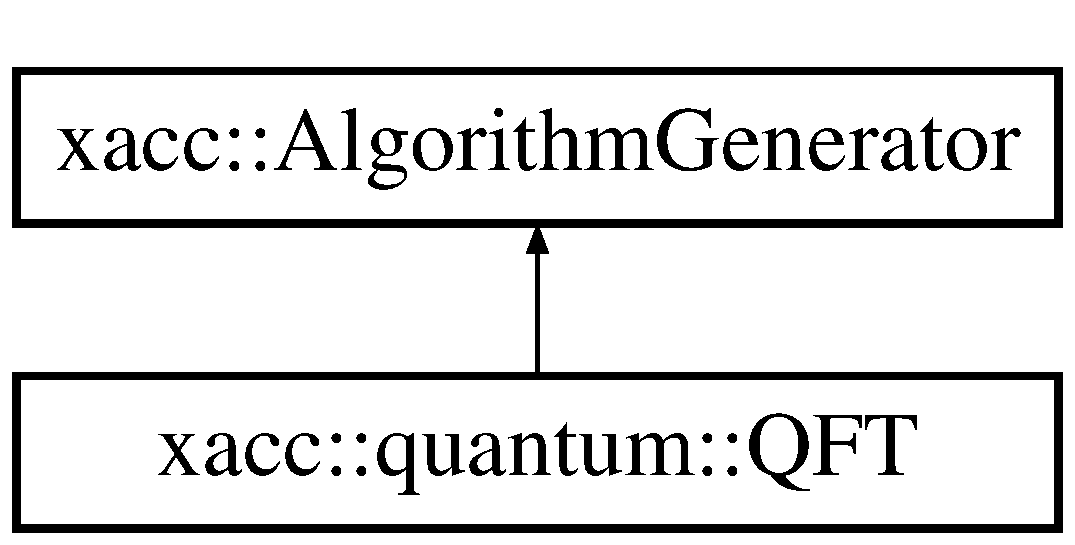
\includegraphics[height=2.000000cm]{a00060}
\end{center}
\end{figure}
\subsection*{Public Member Functions}
\begin{DoxyCompactItemize}
\item 
virtual std\+::shared\+\_\+ptr$<$ \hyperlink{a00038}{Function} $>$ \hyperlink{a00060_ac093c288bc9fc069464fc3fd2cc0ac21}{generate\+Algorithm} (std\+::vector$<$ int $>$ qubits)
\item 
virtual \hyperlink{a00060_a2f585738386f9a3744498983cd1f094e}{$\sim$\+Q\+FT} ()
\end{DoxyCompactItemize}


\subsection{Detailed Description}
\hyperlink{a00060}{Q\+FT} is a realization of the \hyperlink{a00014}{Algorithm\+Generator} interface that produces an X\+A\+CC \hyperlink{a00050}{IR} representation of the Quantum Fourier Transform.

\begin{DoxyAuthor}{Author}
Alex Mc\+Caskey 
\end{DoxyAuthor}


\subsection{Constructor \& Destructor Documentation}
\index{xacc\+::quantum\+::\+Q\+FT@{xacc\+::quantum\+::\+Q\+FT}!````~Q\+FT@{$\sim$\+Q\+FT}}
\index{````~Q\+FT@{$\sim$\+Q\+FT}!xacc\+::quantum\+::\+Q\+FT@{xacc\+::quantum\+::\+Q\+FT}}
\subsubsection[{\texorpdfstring{$\sim$\+Q\+F\+T()}{~QFT()}}]{\setlength{\rightskip}{0pt plus 5cm}virtual xacc\+::quantum\+::\+Q\+F\+T\+::$\sim$\+Q\+FT (
\begin{DoxyParamCaption}
{}
\end{DoxyParamCaption}
)\hspace{0.3cm}{\ttfamily [inline]}, {\ttfamily [virtual]}}\hypertarget{a00060_a2f585738386f9a3744498983cd1f094e}{}\label{a00060_a2f585738386f9a3744498983cd1f094e}
The destructor 

\subsection{Member Function Documentation}
\index{xacc\+::quantum\+::\+Q\+FT@{xacc\+::quantum\+::\+Q\+FT}!generate\+Algorithm@{generate\+Algorithm}}
\index{generate\+Algorithm@{generate\+Algorithm}!xacc\+::quantum\+::\+Q\+FT@{xacc\+::quantum\+::\+Q\+FT}}
\subsubsection[{\texorpdfstring{generate\+Algorithm(std\+::vector$<$ int $>$ qubits)}{generateAlgorithm(std::vector< int > qubits)}}]{\setlength{\rightskip}{0pt plus 5cm}std\+::shared\+\_\+ptr$<$ {\bf Function} $>$ xacc\+::quantum\+::\+Q\+F\+T\+::generate\+Algorithm (
\begin{DoxyParamCaption}
\item[{std\+::vector$<$ int $>$}]{qubits}
\end{DoxyParamCaption}
)\hspace{0.3cm}{\ttfamily [virtual]}}\hypertarget{a00060_ac093c288bc9fc069464fc3fd2cc0ac21}{}\label{a00060_ac093c288bc9fc069464fc3fd2cc0ac21}
This implementation returns a \hyperlink{a00038}{Function} \hyperlink{a00050}{IR} representation of the quantum fourier transform.


\begin{DoxyParams}{Parameters}
{\em bits} & The bits this algorithm operates on \\
\hline
\end{DoxyParams}
\begin{DoxyReturn}{Returns}
function The algorithm represented as an \hyperlink{a00050}{IR} \hyperlink{a00038}{Function} 
\end{DoxyReturn}


Implements \hyperlink{a00014_a73023c06f0f0c62ad56ab4187b18b096}{xacc\+::\+Algorithm\+Generator}.



The documentation for this class was generated from the following files\+:\begin{DoxyCompactItemize}
\item 
Q\+F\+T.\+hpp\item 
Q\+F\+T.\+cpp\end{DoxyCompactItemize}

\hypertarget{a00061}{}\section{xacc\+:\+:quantum\+:\+:Quantum\+Circuit Class Reference}
\label{a00061}\index{xacc\+::quantum\+::\+Quantum\+Circuit@{xacc\+::quantum\+::\+Quantum\+Circuit}}


{\ttfamily \#include $<$Quantum\+Circuit.\+hpp$>$}

Inheritance diagram for xacc\+:\+:quantum\+:\+:Quantum\+Circuit\+:\begin{figure}[H]
\begin{center}
\leavevmode
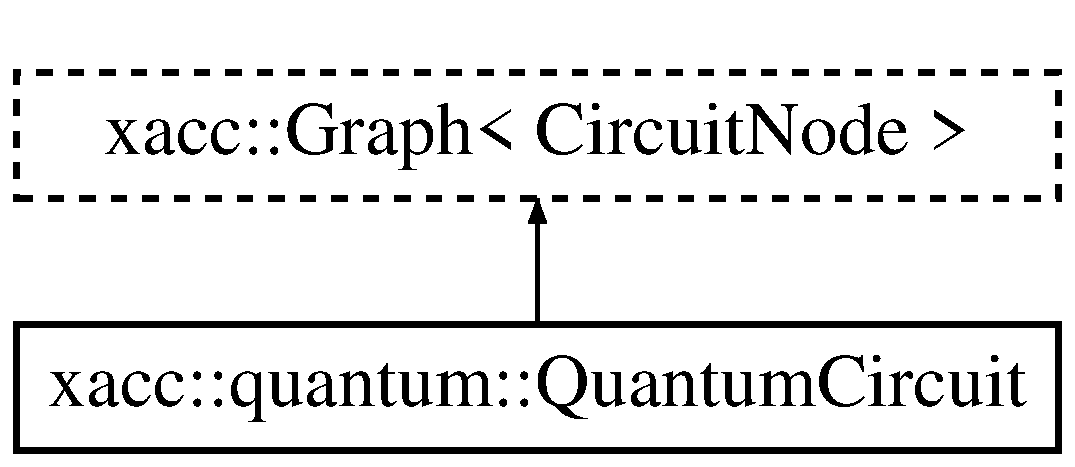
\includegraphics[height=2.000000cm]{a00061}
\end{center}
\end{figure}
\subsection*{Public Member Functions}
\begin{DoxyCompactItemize}
\item 
virtual void \hyperlink{a00061_af7a7f4a487d493fe8a4ed1f76cefd731}{read} (std\+::istream \&stream)
\end{DoxyCompactItemize}
\subsection*{Additional Inherited Members}


\subsection{Detailed Description}
The \hyperlink{a00061}{Quantum\+Circuit} is a subclass of \hyperlink{a00043}{Graph} that provides its Vertex template parameter as a \hyperlink{a00020}{Circuit\+Node}. It adds the ability to read Quantum\+Circuits from a graphviz dot file. 

\subsection{Member Function Documentation}
\index{xacc\+::quantum\+::\+Quantum\+Circuit@{xacc\+::quantum\+::\+Quantum\+Circuit}!read@{read}}
\index{read@{read}!xacc\+::quantum\+::\+Quantum\+Circuit@{xacc\+::quantum\+::\+Quantum\+Circuit}}
\subsubsection[{\texorpdfstring{read(std\+::istream \&stream)}{read(std::istream \&stream)}}]{\setlength{\rightskip}{0pt plus 5cm}virtual void xacc\+::quantum\+::\+Quantum\+Circuit\+::read (
\begin{DoxyParamCaption}
\item[{std\+::istream \&}]{stream}
\end{DoxyParamCaption}
)\hspace{0.3cm}{\ttfamily [inline]}, {\ttfamily [virtual]}}\hypertarget{a00061_af7a7f4a487d493fe8a4ed1f76cefd731}{}\label{a00061_af7a7f4a487d493fe8a4ed1f76cefd731}
Read in a graphviz dot graph from the given input stream. This is left for subclasses.


\begin{DoxyParams}{Parameters}
{\em stream} & \\
\hline
\end{DoxyParams}


Reimplemented from \hyperlink{a00043_abdd3e67dc08c223821d809bc8914164a}{xacc\+::\+Graph$<$ Circuit\+Node $>$}.



The documentation for this class was generated from the following file\+:\begin{DoxyCompactItemize}
\item 
Quantum\+Circuit.\+hpp\end{DoxyCompactItemize}

\hypertarget{a00062}{}\section{xacc\+:\+:quantum\+:\+:Quil\+Compiler Class Reference}
\label{a00062}\index{xacc\+::quantum\+::\+Quil\+Compiler@{xacc\+::quantum\+::\+Quil\+Compiler}}
Inheritance diagram for xacc\+:\+:quantum\+:\+:Quil\+Compiler\+:\begin{figure}[H]
\begin{center}
\leavevmode
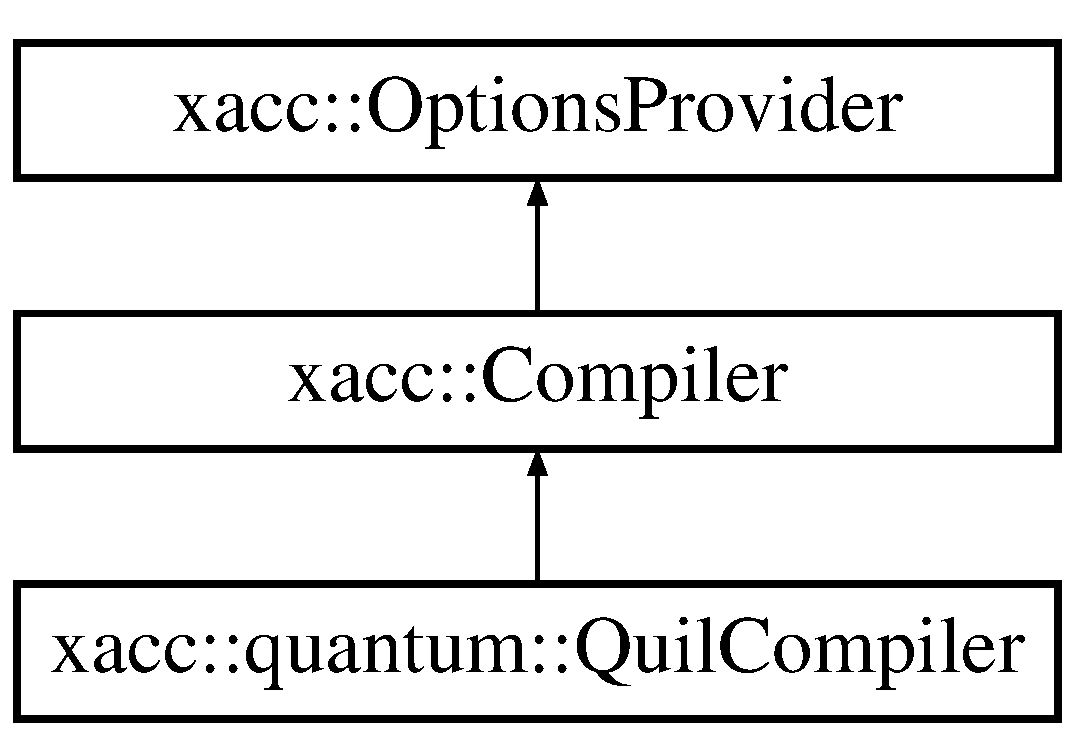
\includegraphics[height=3.000000cm]{a00062}
\end{center}
\end{figure}
\subsection*{Public Member Functions}
\begin{DoxyCompactItemize}
\item 
virtual std\+::shared\+\_\+ptr$<$ \hyperlink{a00050}{xacc\+::\+IR} $>$ \hyperlink{a00062_a2421482415ca4e09963ea4ecddff8100}{compile} (const std\+::string \&src, std\+::shared\+\_\+ptr$<$ \hyperlink{a00011}{Accelerator} $>$ acc)
\item 
virtual std\+::shared\+\_\+ptr$<$ \hyperlink{a00050}{xacc\+::\+IR} $>$ \hyperlink{a00062_adf4d321ecb0df3fa7728999f941c83b2}{compile} (const std\+::string \&src)
\item 
virtual const std\+::string \hyperlink{a00062_ae7d52140b6dd52730edc6e38ae48f437}{get\+Name} ()
\item 
virtual const std\+::string \hyperlink{a00062_a66ca00bbb1f30e7bc6dd86b1e267b93b}{translate} (const std\+::string \&buffer\+Variable, std\+::shared\+\_\+ptr$<$ \hyperlink{a00038}{Function} $>$ function)
\item 
virtual \hyperlink{a00062_a0866a9f695f28c90ac1f4754374f3bfe}{$\sim$\+Quil\+Compiler} ()
\end{DoxyCompactItemize}
\subsection*{Static Public Member Functions}
\begin{DoxyCompactItemize}
\item 
static void \hyperlink{a00062_aaec99a14bede717bf02a0f65af2a3c69}{register\+Compiler} ()
\end{DoxyCompactItemize}
\subsection*{Additional Inherited Members}


\subsection{Constructor \& Destructor Documentation}
\index{xacc\+::quantum\+::\+Quil\+Compiler@{xacc\+::quantum\+::\+Quil\+Compiler}!````~Quil\+Compiler@{$\sim$\+Quil\+Compiler}}
\index{````~Quil\+Compiler@{$\sim$\+Quil\+Compiler}!xacc\+::quantum\+::\+Quil\+Compiler@{xacc\+::quantum\+::\+Quil\+Compiler}}
\subsubsection[{\texorpdfstring{$\sim$\+Quil\+Compiler()}{~QuilCompiler()}}]{\setlength{\rightskip}{0pt plus 5cm}virtual xacc\+::quantum\+::\+Quil\+Compiler\+::$\sim$\+Quil\+Compiler (
\begin{DoxyParamCaption}
{}
\end{DoxyParamCaption}
)\hspace{0.3cm}{\ttfamily [inline]}, {\ttfamily [virtual]}}\hypertarget{a00062_a0866a9f695f28c90ac1f4754374f3bfe}{}\label{a00062_a0866a9f695f28c90ac1f4754374f3bfe}
The destructor 

\subsection{Member Function Documentation}
\index{xacc\+::quantum\+::\+Quil\+Compiler@{xacc\+::quantum\+::\+Quil\+Compiler}!compile@{compile}}
\index{compile@{compile}!xacc\+::quantum\+::\+Quil\+Compiler@{xacc\+::quantum\+::\+Quil\+Compiler}}
\subsubsection[{\texorpdfstring{compile(const std\+::string \&src, std\+::shared\+\_\+ptr$<$ Accelerator $>$ acc)}{compile(const std::string \&src, std::shared\_ptr< Accelerator > acc)}}]{\setlength{\rightskip}{0pt plus 5cm}std\+::shared\+\_\+ptr$<$ {\bf IR} $>$ xacc\+::quantum\+::\+Quil\+Compiler\+::compile (
\begin{DoxyParamCaption}
\item[{const std\+::string \&}]{src, }
\item[{std\+::shared\+\_\+ptr$<$ {\bf Accelerator} $>$}]{acc}
\end{DoxyParamCaption}
)\hspace{0.3cm}{\ttfamily [virtual]}}\hypertarget{a00062_a2421482415ca4e09963ea4ecddff8100}{}\label{a00062_a2421482415ca4e09963ea4ecddff8100}
Translate Quil to the X\+A\+CC intermediate representation.

\begin{DoxyReturn}{Returns}
ir X\+A\+CC intermediate representation 
\end{DoxyReturn}


Implements \hyperlink{a00023_a546a40c95bb93af6a0c0ac48dbeaffc8}{xacc\+::\+Compiler}.

\index{xacc\+::quantum\+::\+Quil\+Compiler@{xacc\+::quantum\+::\+Quil\+Compiler}!compile@{compile}}
\index{compile@{compile}!xacc\+::quantum\+::\+Quil\+Compiler@{xacc\+::quantum\+::\+Quil\+Compiler}}
\subsubsection[{\texorpdfstring{compile(const std\+::string \&src)}{compile(const std::string \&src)}}]{\setlength{\rightskip}{0pt plus 5cm}std\+::shared\+\_\+ptr$<$ {\bf IR} $>$ xacc\+::quantum\+::\+Quil\+Compiler\+::compile (
\begin{DoxyParamCaption}
\item[{const std\+::string \&}]{src}
\end{DoxyParamCaption}
)\hspace{0.3cm}{\ttfamily [virtual]}}\hypertarget{a00062_adf4d321ecb0df3fa7728999f941c83b2}{}\label{a00062_adf4d321ecb0df3fa7728999f941c83b2}

\begin{DoxyParams}{Parameters}
{\em src} & \\
\hline
\end{DoxyParams}
\begin{DoxyReturn}{Returns}

\end{DoxyReturn}


Implements \hyperlink{a00023_a9092f5f779b570c91569b59621280c04}{xacc\+::\+Compiler}.

\index{xacc\+::quantum\+::\+Quil\+Compiler@{xacc\+::quantum\+::\+Quil\+Compiler}!get\+Name@{get\+Name}}
\index{get\+Name@{get\+Name}!xacc\+::quantum\+::\+Quil\+Compiler@{xacc\+::quantum\+::\+Quil\+Compiler}}
\subsubsection[{\texorpdfstring{get\+Name()}{getName()}}]{\setlength{\rightskip}{0pt plus 5cm}virtual const std\+::string xacc\+::quantum\+::\+Quil\+Compiler\+::get\+Name (
\begin{DoxyParamCaption}
{}
\end{DoxyParamCaption}
)\hspace{0.3cm}{\ttfamily [inline]}, {\ttfamily [virtual]}}\hypertarget{a00062_ae7d52140b6dd52730edc6e38ae48f437}{}\label{a00062_ae7d52140b6dd52730edc6e38ae48f437}
Return the name of this \hyperlink{a00023}{Compiler} \begin{DoxyReturn}{Returns}
name \hyperlink{a00023}{Compiler} name 
\end{DoxyReturn}


Implements \hyperlink{a00023_a87fca9100e6462122f5b687c3a0fb3fb}{xacc\+::\+Compiler}.

\index{xacc\+::quantum\+::\+Quil\+Compiler@{xacc\+::quantum\+::\+Quil\+Compiler}!register\+Compiler@{register\+Compiler}}
\index{register\+Compiler@{register\+Compiler}!xacc\+::quantum\+::\+Quil\+Compiler@{xacc\+::quantum\+::\+Quil\+Compiler}}
\subsubsection[{\texorpdfstring{register\+Compiler()}{registerCompiler()}}]{\setlength{\rightskip}{0pt plus 5cm}static void xacc\+::quantum\+::\+Quil\+Compiler\+::register\+Compiler (
\begin{DoxyParamCaption}
{}
\end{DoxyParamCaption}
)\hspace{0.3cm}{\ttfamily [inline]}, {\ttfamily [static]}}\hypertarget{a00062_aaec99a14bede717bf02a0f65af2a3c69}{}\label{a00062_aaec99a14bede717bf02a0f65af2a3c69}
Register this \hyperlink{a00023}{Compiler} with the framework. \index{xacc\+::quantum\+::\+Quil\+Compiler@{xacc\+::quantum\+::\+Quil\+Compiler}!translate@{translate}}
\index{translate@{translate}!xacc\+::quantum\+::\+Quil\+Compiler@{xacc\+::quantum\+::\+Quil\+Compiler}}
\subsubsection[{\texorpdfstring{translate(const std\+::string \&buffer\+Variable, std\+::shared\+\_\+ptr$<$ Function $>$ function)}{translate(const std::string \&bufferVariable, std::shared\_ptr< Function > function)}}]{\setlength{\rightskip}{0pt plus 5cm}const std\+::string xacc\+::quantum\+::\+Quil\+Compiler\+::translate (
\begin{DoxyParamCaption}
\item[{const std\+::string \&}]{buffer\+Variable, }
\item[{std\+::shared\+\_\+ptr$<$ {\bf Function} $>$}]{function}
\end{DoxyParamCaption}
)\hspace{0.3cm}{\ttfamily [virtual]}}\hypertarget{a00062_a66ca00bbb1f30e7bc6dd86b1e267b93b}{}\label{a00062_a66ca00bbb1f30e7bc6dd86b1e267b93b}
This produces a Quil source code representation of the given \hyperlink{a00050}{IR} \hyperlink{a00038}{Function}


\begin{DoxyParams}{Parameters}
{\em function} & The X\+A\+CC \hyperlink{a00050}{IR} \hyperlink{a00038}{Function} to translate \\
\hline
\end{DoxyParams}
\begin{DoxyReturn}{Returns}
src The source code as a string 
\end{DoxyReturn}


Implements \hyperlink{a00023_aeedbe58a33fed29e4d7694ae743e25e7}{xacc\+::\+Compiler}.



The documentation for this class was generated from the following files\+:\begin{DoxyCompactItemize}
\item 
Quil\+Compiler.\+hpp\item 
Quil\+Compiler.\+cpp\end{DoxyCompactItemize}

\hypertarget{a00063}{}\section{xacc\+:\+:quantum\+:\+:Quil\+Visitor Class Reference}
\label{a00063}\index{xacc\+::quantum\+::\+Quil\+Visitor@{xacc\+::quantum\+::\+Quil\+Visitor}}


{\ttfamily \#include $<$Quil\+Visitor.\+hpp$>$}

Inheritance diagram for xacc\+:\+:quantum\+:\+:Quil\+Visitor\+:\begin{figure}[H]
\begin{center}
\leavevmode
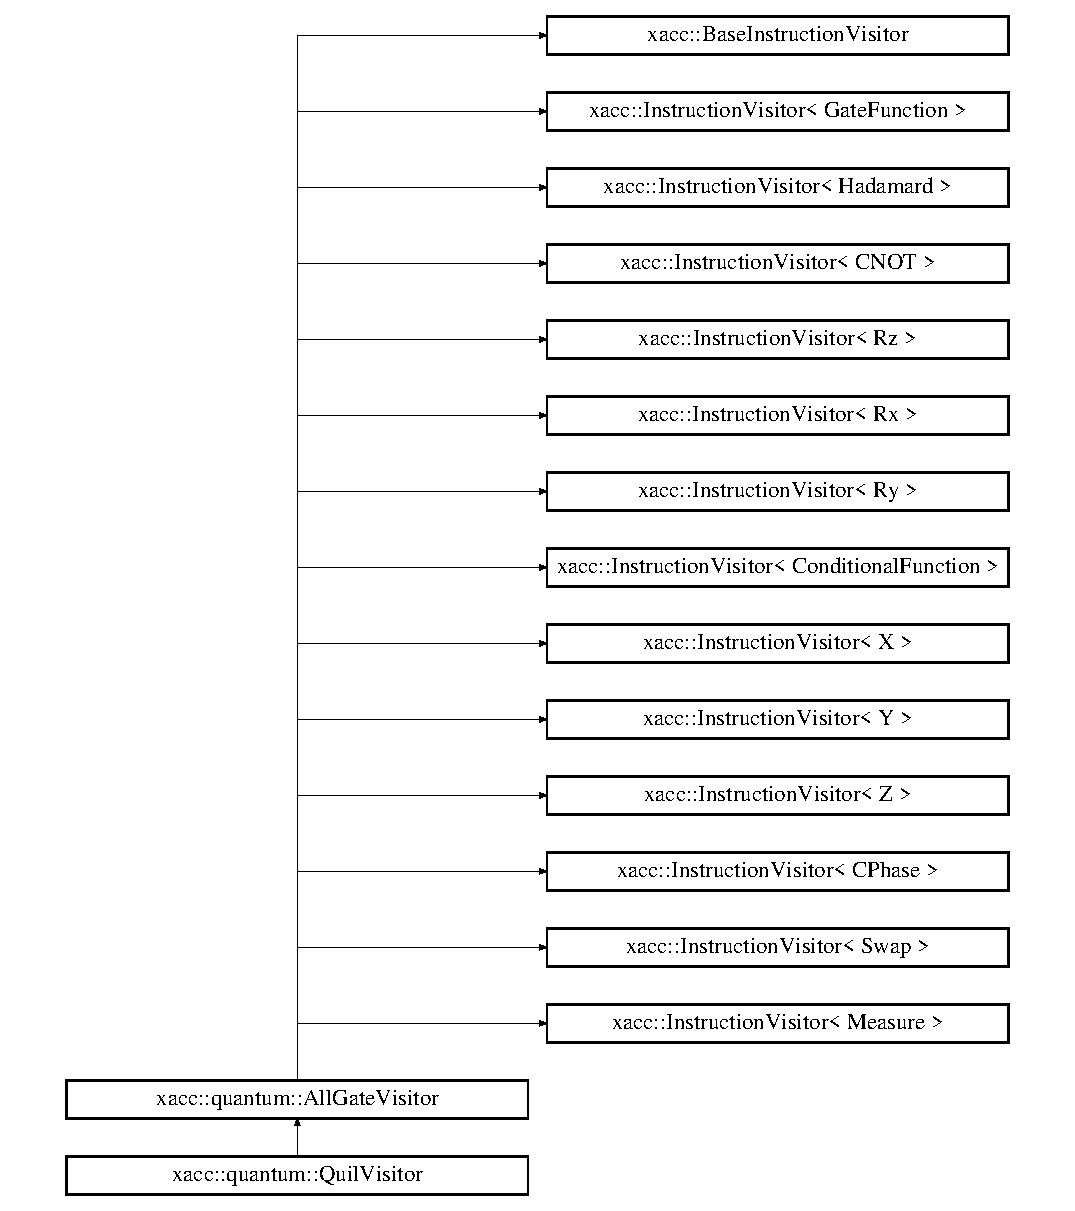
\includegraphics[height=12.000000cm]{a00063}
\end{center}
\end{figure}
\subsection*{Public Member Functions}
\begin{DoxyCompactItemize}
\item 
void \hyperlink{a00063_a5470d573fdcfd691c100fcbfeeed45db}{visit} (\hyperlink{a00044}{Hadamard} \&h)
\item 
void \hyperlink{a00063_ac51ed9d947d3fa00525eb79b2bbc9021}{visit} (\hyperlink{a00022}{C\+N\+OT} \&cn)
\item 
void \hyperlink{a00063_a0b1a31a900f87a3f91f640ab5caec126}{visit} (\hyperlink{a00084}{X} \&x)
\item 
void {\bfseries visit} (\hyperlink{a00087}{Y} \&y)\hypertarget{a00063_a403f2d506425ee5a0098b1b54de7e4e8}{}\label{a00063_a403f2d506425ee5a0098b1b54de7e4e8}

\item 
void \hyperlink{a00063_af429121067a397eeac17328fc0244859}{visit} (\hyperlink{a00088}{Z} \&z)
\item 
void \hyperlink{a00063_acbe2afe1c9741112d1f9196681f8b896}{visit} (\hyperlink{a00055}{Measure} \&m)
\item 
void \hyperlink{a00063_a7665ecdf9984374f52d30d7767649cf9}{visit} (\hyperlink{a00025}{Conditional\+Function} \&c)
\item 
void {\bfseries visit} (\hyperlink{a00073}{Rx} \&rx)\hypertarget{a00063_a81a75fb24d368aeb8396d2cbde0bbfb4}{}\label{a00063_a81a75fb24d368aeb8396d2cbde0bbfb4}

\item 
void {\bfseries visit} (\hyperlink{a00074}{Ry} \&ry)\hypertarget{a00063_ad74c7ec734670c2a5478ebb40e097bfc}{}\label{a00063_ad74c7ec734670c2a5478ebb40e097bfc}

\item 
void {\bfseries visit} (\hyperlink{a00075}{Rz} \&rz)\hypertarget{a00063_aa3823bdeb4d930f753d4b421730c5912}{}\label{a00063_aa3823bdeb4d930f753d4b421730c5912}

\item 
void {\bfseries visit} (\hyperlink{a00027}{C\+Phase} \&cp)\hypertarget{a00063_a7a043f72038fec08ac64d375a663e96d}{}\label{a00063_a7a043f72038fec08ac64d375a663e96d}

\item 
void {\bfseries visit} (\hyperlink{a00082}{Swap} \&s)\hypertarget{a00063_a2b822a63888043498203dd0b0c935a51}{}\label{a00063_a2b822a63888043498203dd0b0c935a51}

\item 
void {\bfseries visit} (\hyperlink{a00040}{Gate\+Function} \&f)\hypertarget{a00063_addedb7635dd200885904611e4cae39d4}{}\label{a00063_addedb7635dd200885904611e4cae39d4}

\item 
std\+::string \hyperlink{a00063_a9808ecc5766ea2c387107dff6b64cdb8}{get\+Quil\+String} ()
\item 
std\+::string \hyperlink{a00063_ab4a1c6a92772a09c22068ced7d3dc76c}{get\+Classical\+Addresses} ()
\item 
int {\bfseries get\+Number\+Of\+Addresses} ()\hypertarget{a00063_a561aabf6de48ae9aee4fbe868f1c5da1}{}\label{a00063_a561aabf6de48ae9aee4fbe868f1c5da1}

\item 
virtual \hyperlink{a00063_a90dcced4e75c7b45c287fb4edc58ed01}{$\sim$\+Quil\+Visitor} ()
\end{DoxyCompactItemize}
\subsection*{Protected Attributes}
\begin{DoxyCompactItemize}
\item 
std\+::string \hyperlink{a00063_afd04300ce4dab03448a09f9bee448ca6}{quil\+Str}
\item 
std\+::string \hyperlink{a00063_a93e648797062568ff2ae0345f8843ddd}{classical\+Addresses}
\item 
std\+::map$<$ int, int $>$ {\bfseries qubit\+To\+Classical\+Bit\+Index}\hypertarget{a00063_abc613802d6ea40a54c6e75df227a28bb}{}\label{a00063_abc613802d6ea40a54c6e75df227a28bb}

\item 
int {\bfseries num\+Addresses} = 0\hypertarget{a00063_ada92b9a834de74d79c22e1c5e88509ec}{}\label{a00063_ada92b9a834de74d79c22e1c5e88509ec}

\end{DoxyCompactItemize}


\subsection{Detailed Description}
The \hyperlink{a00063}{Quil\+Visitor} is an \hyperlink{a00048}{Instruction\+Visitor} that visits quantum gate instructions and creates an equivalent Quil string that can be executed by the Rigetti superconducting quantum computer. 

\subsection{Constructor \& Destructor Documentation}
\index{xacc\+::quantum\+::\+Quil\+Visitor@{xacc\+::quantum\+::\+Quil\+Visitor}!````~Quil\+Visitor@{$\sim$\+Quil\+Visitor}}
\index{````~Quil\+Visitor@{$\sim$\+Quil\+Visitor}!xacc\+::quantum\+::\+Quil\+Visitor@{xacc\+::quantum\+::\+Quil\+Visitor}}
\subsubsection[{\texorpdfstring{$\sim$\+Quil\+Visitor()}{~QuilVisitor()}}]{\setlength{\rightskip}{0pt plus 5cm}virtual xacc\+::quantum\+::\+Quil\+Visitor\+::$\sim$\+Quil\+Visitor (
\begin{DoxyParamCaption}
{}
\end{DoxyParamCaption}
)\hspace{0.3cm}{\ttfamily [inline]}, {\ttfamily [virtual]}}\hypertarget{a00063_a90dcced4e75c7b45c287fb4edc58ed01}{}\label{a00063_a90dcced4e75c7b45c287fb4edc58ed01}
The destructor 

\subsection{Member Function Documentation}
\index{xacc\+::quantum\+::\+Quil\+Visitor@{xacc\+::quantum\+::\+Quil\+Visitor}!get\+Classical\+Addresses@{get\+Classical\+Addresses}}
\index{get\+Classical\+Addresses@{get\+Classical\+Addresses}!xacc\+::quantum\+::\+Quil\+Visitor@{xacc\+::quantum\+::\+Quil\+Visitor}}
\subsubsection[{\texorpdfstring{get\+Classical\+Addresses()}{getClassicalAddresses()}}]{\setlength{\rightskip}{0pt plus 5cm}std\+::string xacc\+::quantum\+::\+Quil\+Visitor\+::get\+Classical\+Addresses (
\begin{DoxyParamCaption}
{}
\end{DoxyParamCaption}
)\hspace{0.3cm}{\ttfamily [inline]}}\hypertarget{a00063_ab4a1c6a92772a09c22068ced7d3dc76c}{}\label{a00063_ab4a1c6a92772a09c22068ced7d3dc76c}
Return the classical measurement indices as a json int array represented as a string. \index{xacc\+::quantum\+::\+Quil\+Visitor@{xacc\+::quantum\+::\+Quil\+Visitor}!get\+Quil\+String@{get\+Quil\+String}}
\index{get\+Quil\+String@{get\+Quil\+String}!xacc\+::quantum\+::\+Quil\+Visitor@{xacc\+::quantum\+::\+Quil\+Visitor}}
\subsubsection[{\texorpdfstring{get\+Quil\+String()}{getQuilString()}}]{\setlength{\rightskip}{0pt plus 5cm}std\+::string xacc\+::quantum\+::\+Quil\+Visitor\+::get\+Quil\+String (
\begin{DoxyParamCaption}
{}
\end{DoxyParamCaption}
)\hspace{0.3cm}{\ttfamily [inline]}}\hypertarget{a00063_a9808ecc5766ea2c387107dff6b64cdb8}{}\label{a00063_a9808ecc5766ea2c387107dff6b64cdb8}
Return the quil string \index{xacc\+::quantum\+::\+Quil\+Visitor@{xacc\+::quantum\+::\+Quil\+Visitor}!visit@{visit}}
\index{visit@{visit}!xacc\+::quantum\+::\+Quil\+Visitor@{xacc\+::quantum\+::\+Quil\+Visitor}}
\subsubsection[{\texorpdfstring{visit(\+Hadamard \&h)}{visit(Hadamard \&h)}}]{\setlength{\rightskip}{0pt plus 5cm}void xacc\+::quantum\+::\+Quil\+Visitor\+::visit (
\begin{DoxyParamCaption}
\item[{{\bf Hadamard} \&}]{h}
\end{DoxyParamCaption}
)\hspace{0.3cm}{\ttfamily [inline]}}\hypertarget{a00063_a5470d573fdcfd691c100fcbfeeed45db}{}\label{a00063_a5470d573fdcfd691c100fcbfeeed45db}
Visit hadamard gates \index{xacc\+::quantum\+::\+Quil\+Visitor@{xacc\+::quantum\+::\+Quil\+Visitor}!visit@{visit}}
\index{visit@{visit}!xacc\+::quantum\+::\+Quil\+Visitor@{xacc\+::quantum\+::\+Quil\+Visitor}}
\subsubsection[{\texorpdfstring{visit(\+C\+N\+O\+T \&cn)}{visit(CNOT \&cn)}}]{\setlength{\rightskip}{0pt plus 5cm}void xacc\+::quantum\+::\+Quil\+Visitor\+::visit (
\begin{DoxyParamCaption}
\item[{{\bf C\+N\+OT} \&}]{cn}
\end{DoxyParamCaption}
)\hspace{0.3cm}{\ttfamily [inline]}}\hypertarget{a00063_ac51ed9d947d3fa00525eb79b2bbc9021}{}\label{a00063_ac51ed9d947d3fa00525eb79b2bbc9021}
Visit \hyperlink{a00022}{C\+N\+OT} gates \index{xacc\+::quantum\+::\+Quil\+Visitor@{xacc\+::quantum\+::\+Quil\+Visitor}!visit@{visit}}
\index{visit@{visit}!xacc\+::quantum\+::\+Quil\+Visitor@{xacc\+::quantum\+::\+Quil\+Visitor}}
\subsubsection[{\texorpdfstring{visit(\+X \&x)}{visit(X \&x)}}]{\setlength{\rightskip}{0pt plus 5cm}void xacc\+::quantum\+::\+Quil\+Visitor\+::visit (
\begin{DoxyParamCaption}
\item[{{\bf X} \&}]{x}
\end{DoxyParamCaption}
)\hspace{0.3cm}{\ttfamily [inline]}}\hypertarget{a00063_a0b1a31a900f87a3f91f640ab5caec126}{}\label{a00063_a0b1a31a900f87a3f91f640ab5caec126}
Visit \hyperlink{a00084}{X} gates \index{xacc\+::quantum\+::\+Quil\+Visitor@{xacc\+::quantum\+::\+Quil\+Visitor}!visit@{visit}}
\index{visit@{visit}!xacc\+::quantum\+::\+Quil\+Visitor@{xacc\+::quantum\+::\+Quil\+Visitor}}
\subsubsection[{\texorpdfstring{visit(\+Z \&z)}{visit(Z \&z)}}]{\setlength{\rightskip}{0pt plus 5cm}void xacc\+::quantum\+::\+Quil\+Visitor\+::visit (
\begin{DoxyParamCaption}
\item[{{\bf Z} \&}]{z}
\end{DoxyParamCaption}
)\hspace{0.3cm}{\ttfamily [inline]}}\hypertarget{a00063_af429121067a397eeac17328fc0244859}{}\label{a00063_af429121067a397eeac17328fc0244859}
Visit \hyperlink{a00088}{Z} gates \index{xacc\+::quantum\+::\+Quil\+Visitor@{xacc\+::quantum\+::\+Quil\+Visitor}!visit@{visit}}
\index{visit@{visit}!xacc\+::quantum\+::\+Quil\+Visitor@{xacc\+::quantum\+::\+Quil\+Visitor}}
\subsubsection[{\texorpdfstring{visit(\+Measure \&m)}{visit(Measure \&m)}}]{\setlength{\rightskip}{0pt plus 5cm}void xacc\+::quantum\+::\+Quil\+Visitor\+::visit (
\begin{DoxyParamCaption}
\item[{{\bf Measure} \&}]{m}
\end{DoxyParamCaption}
)\hspace{0.3cm}{\ttfamily [inline]}}\hypertarget{a00063_acbe2afe1c9741112d1f9196681f8b896}{}\label{a00063_acbe2afe1c9741112d1f9196681f8b896}
Visit Measurement gates \index{xacc\+::quantum\+::\+Quil\+Visitor@{xacc\+::quantum\+::\+Quil\+Visitor}!visit@{visit}}
\index{visit@{visit}!xacc\+::quantum\+::\+Quil\+Visitor@{xacc\+::quantum\+::\+Quil\+Visitor}}
\subsubsection[{\texorpdfstring{visit(\+Conditional\+Function \&c)}{visit(ConditionalFunction \&c)}}]{\setlength{\rightskip}{0pt plus 5cm}void xacc\+::quantum\+::\+Quil\+Visitor\+::visit (
\begin{DoxyParamCaption}
\item[{{\bf Conditional\+Function} \&}]{c}
\end{DoxyParamCaption}
)\hspace{0.3cm}{\ttfamily [inline]}}\hypertarget{a00063_a7665ecdf9984374f52d30d7767649cf9}{}\label{a00063_a7665ecdf9984374f52d30d7767649cf9}
Visit Conditional functions 

\subsection{Member Data Documentation}
\index{xacc\+::quantum\+::\+Quil\+Visitor@{xacc\+::quantum\+::\+Quil\+Visitor}!classical\+Addresses@{classical\+Addresses}}
\index{classical\+Addresses@{classical\+Addresses}!xacc\+::quantum\+::\+Quil\+Visitor@{xacc\+::quantum\+::\+Quil\+Visitor}}
\subsubsection[{\texorpdfstring{classical\+Addresses}{classicalAddresses}}]{\setlength{\rightskip}{0pt plus 5cm}std\+::string xacc\+::quantum\+::\+Quil\+Visitor\+::classical\+Addresses\hspace{0.3cm}{\ttfamily [protected]}}\hypertarget{a00063_a93e648797062568ff2ae0345f8843ddd}{}\label{a00063_a93e648797062568ff2ae0345f8843ddd}
Reference to the classical memory address indices where measurements are recorded. \index{xacc\+::quantum\+::\+Quil\+Visitor@{xacc\+::quantum\+::\+Quil\+Visitor}!quil\+Str@{quil\+Str}}
\index{quil\+Str@{quil\+Str}!xacc\+::quantum\+::\+Quil\+Visitor@{xacc\+::quantum\+::\+Quil\+Visitor}}
\subsubsection[{\texorpdfstring{quil\+Str}{quilStr}}]{\setlength{\rightskip}{0pt plus 5cm}std\+::string xacc\+::quantum\+::\+Quil\+Visitor\+::quil\+Str\hspace{0.3cm}{\ttfamily [protected]}}\hypertarget{a00063_afd04300ce4dab03448a09f9bee448ca6}{}\label{a00063_afd04300ce4dab03448a09f9bee448ca6}
Reference to the Quil string this visitor is trying to construct 

The documentation for this class was generated from the following file\+:\begin{DoxyCompactItemize}
\item 
Quil\+Visitor.\+hpp\end{DoxyCompactItemize}

\hypertarget{a00064}{}\section{xacc\+:\+:Register\+Accelerator$<$ T $>$ Class Template Reference}
\label{a00064}\index{xacc\+::\+Register\+Accelerator$<$ T $>$@{xacc\+::\+Register\+Accelerator$<$ T $>$}}


{\ttfamily \#include $<$Accelerator.\+hpp$>$}

\subsection*{Public Member Functions}
\begin{DoxyCompactItemize}
\item 
{\bfseries Register\+Accelerator} (const std\+::string \&name)\hypertarget{a00064_a329df136d447a887e9794ea078d04706}{}\label{a00064_a329df136d447a887e9794ea078d04706}

\item 
{\bfseries Register\+Accelerator} (const std\+::string \&name, std\+::shared\+\_\+ptr$<$ options\+\_\+description $>$ options)\hypertarget{a00064_a753204b9774ff46ff5443a9709f46eed}{}\label{a00064_a753204b9774ff46ff5443a9709f46eed}

\end{DoxyCompactItemize}


\subsection{Detailed Description}
\subsubsection*{template$<$typename T$>$\\*
class xacc\+::\+Register\+Accelerator$<$ T $>$}

\hyperlink{a00064}{Register\+Accelerator} is a convenience class for registering custom derived \hyperlink{a00011}{Accelerator} classes.

Creators of \hyperlink{a00011}{Accelerator} subclasses create an instance of this class with their \hyperlink{a00011}{Accelerator} subclass as the template parameter to register their \hyperlink{a00011}{Accelerator} with X\+A\+CC. This instance must be created in the C\+PP implementation file for the \hyperlink{a00011}{Accelerator} and at global scope. 

The documentation for this class was generated from the following file\+:\begin{DoxyCompactItemize}
\item 
Accelerator.\+hpp\end{DoxyCompactItemize}

\hypertarget{a00065}{}\section{xacc\+:\+:Register\+Algorithm\+Generator$<$ T $>$ Class Template Reference}
\label{a00065}\index{xacc\+::\+Register\+Algorithm\+Generator$<$ T $>$@{xacc\+::\+Register\+Algorithm\+Generator$<$ T $>$}}


{\ttfamily \#include $<$Algorithm\+Generator.\+hpp$>$}

\subsection*{Public Member Functions}
\begin{DoxyCompactItemize}
\item 
{\bfseries Register\+Algorithm\+Generator} (const std\+::string \&name)\hypertarget{a00065_af439cc4d7c8d6628a979129a5c1411df}{}\label{a00065_af439cc4d7c8d6628a979129a5c1411df}

\end{DoxyCompactItemize}


\subsection{Detailed Description}
\subsubsection*{template$<$typename T$>$\\*
class xacc\+::\+Register\+Algorithm\+Generator$<$ T $>$}

\hyperlink{a00065}{Register\+Algorithm\+Generator} is a convenience class for registering custom derived \hyperlink{a00014}{Algorithm\+Generator} classes.

Creators of \hyperlink{a00014}{Algorithm\+Generator} subclasses create an instance of this class with their \hyperlink{a00014}{Algorithm\+Generator} subclass as the template parameter to register their \hyperlink{a00014}{Algorithm\+Generator} with X\+A\+CC. This instance must be created in the C\+PP implementation file for the \hyperlink{a00014}{Algorithm\+Generator} and at global scope. 

The documentation for this class was generated from the following file\+:\begin{DoxyCompactItemize}
\item 
Algorithm\+Generator.\+hpp\end{DoxyCompactItemize}

\hypertarget{a00066}{}\section{xacc\+:\+:Register\+Compiler$<$ T $>$ Class Template Reference}
\label{a00066}\index{xacc\+::\+Register\+Compiler$<$ T $>$@{xacc\+::\+Register\+Compiler$<$ T $>$}}


{\ttfamily \#include $<$Compiler.\+hpp$>$}

\subsection*{Public Member Functions}
\begin{DoxyCompactItemize}
\item 
{\bfseries Register\+Compiler} (const std\+::string \&name)\hypertarget{a00066_a41f5c1abd570b3867b9790cdc02f3355}{}\label{a00066_a41f5c1abd570b3867b9790cdc02f3355}

\item 
{\bfseries Register\+Compiler} (const std\+::string \&name, std\+::shared\+\_\+ptr$<$ options\+\_\+description $>$ options)\hypertarget{a00066_a3489e8cf59f2b0c14e4e2037b61bc368}{}\label{a00066_a3489e8cf59f2b0c14e4e2037b61bc368}

\end{DoxyCompactItemize}


\subsection{Detailed Description}
\subsubsection*{template$<$typename T$>$\\*
class xacc\+::\+Register\+Compiler$<$ T $>$}

\hyperlink{a00066}{Register\+Compiler} is a convenience class for registering custom derived \hyperlink{a00023}{Compiler} classes.

Creators of \hyperlink{a00023}{Compiler} subclasses create an instance of this class with their \hyperlink{a00023}{Compiler} subclass as the template parameter to register their \hyperlink{a00023}{Compiler} with X\+A\+CC. This instance must be created in the C\+PP implementation file for the \hyperlink{a00023}{Compiler} and at global scope. 

The documentation for this class was generated from the following file\+:\begin{DoxyCompactItemize}
\item 
Compiler.\+hpp\end{DoxyCompactItemize}

\hypertarget{a00067}{}\section{xacc\+:\+:quantum\+:\+:Register\+Embedding\+Algorithm$<$ T $>$ Class Template Reference}
\label{a00067}\index{xacc\+::quantum\+::\+Register\+Embedding\+Algorithm$<$ T $>$@{xacc\+::quantum\+::\+Register\+Embedding\+Algorithm$<$ T $>$}}


{\ttfamily \#include $<$Embedding\+Algorithm.\+hpp$>$}

\subsection*{Public Member Functions}
\begin{DoxyCompactItemize}
\item 
{\bfseries Register\+Embedding\+Algorithm} (const std\+::string \&name)\hypertarget{a00067_a0b849a815e56d04c22e04b8c2f43f3d3}{}\label{a00067_a0b849a815e56d04c22e04b8c2f43f3d3}

\end{DoxyCompactItemize}


\subsection{Detailed Description}
\subsubsection*{template$<$typename T$>$\\*
class xacc\+::quantum\+::\+Register\+Embedding\+Algorithm$<$ T $>$}

\hyperlink{a00067}{Register\+Embedding\+Algorithm} is a convenience class for registering custom derived \hyperlink{a00037}{Embedding\+Algorithm} classes.

Creators of \hyperlink{a00037}{Embedding\+Algorithm} subclasses create an instance of this class with their \hyperlink{a00037}{Embedding\+Algorithm} subclass as the template parameter to register their \hyperlink{a00037}{Embedding\+Algorithm} with X\+A\+CC. This instance must be created in the C\+PP implementation file for the \hyperlink{a00037}{Embedding\+Algorithm} and at global scope. 

The documentation for this class was generated from the following file\+:\begin{DoxyCompactItemize}
\item 
Embedding\+Algorithm.\+hpp\end{DoxyCompactItemize}

\hypertarget{a00068}{}\section{xacc\+:\+:quantum\+:\+:Register\+Gate\+Instruction$<$ T $>$ Class Template Reference}
\label{a00068}\index{xacc\+::quantum\+::\+Register\+Gate\+Instruction$<$ T $>$@{xacc\+::quantum\+::\+Register\+Gate\+Instruction$<$ T $>$}}
\subsection*{Public Member Functions}
\begin{DoxyCompactItemize}
\item 
{\bfseries Register\+Gate\+Instruction} (const std\+::string \&name)\hypertarget{a00068_aad394924e098f0cc8da5cc7f211acd7a}{}\label{a00068_aad394924e098f0cc8da5cc7f211acd7a}

\end{DoxyCompactItemize}


The documentation for this class was generated from the following file\+:\begin{DoxyCompactItemize}
\item 
Gate\+Instruction.\+hpp\end{DoxyCompactItemize}

\hypertarget{a00069}{}\section{xacc\+:\+:Register\+Preprocessor$<$ T $>$ Class Template Reference}
\label{a00069}\index{xacc\+::\+Register\+Preprocessor$<$ T $>$@{xacc\+::\+Register\+Preprocessor$<$ T $>$}}


{\ttfamily \#include $<$Preprocessor.\+hpp$>$}

\subsection*{Public Member Functions}
\begin{DoxyCompactItemize}
\item 
{\bfseries Register\+Preprocessor} (const std\+::string \&name)\hypertarget{a00069_a360d5ffa16ef3a96c3bc61fa897ffe3c}{}\label{a00069_a360d5ffa16ef3a96c3bc61fa897ffe3c}

\end{DoxyCompactItemize}


\subsection{Detailed Description}
\subsubsection*{template$<$typename T$>$\\*
class xacc\+::\+Register\+Preprocessor$<$ T $>$}

\hyperlink{a00069}{Register\+Preprocessor} is a convenience class for registering custom derived \hyperlink{a00057}{Preprocessor} classes.

Creators of \hyperlink{a00057}{Preprocessor} subclasses create an instance of this class with their \hyperlink{a00057}{Preprocessor} subclass as the template parameter to register their \hyperlink{a00057}{Preprocessor} with X\+A\+CC. This instance must be created in the C\+PP implementation file for the \hyperlink{a00057}{Preprocessor} and at global scope. 

The documentation for this class was generated from the following file\+:\begin{DoxyCompactItemize}
\item 
Preprocessor.\+hpp\end{DoxyCompactItemize}

\hypertarget{a00070}{}\section{xacc\+:\+:Registry$<$ T, T\+Args $>$ Class Template Reference}
\label{a00070}\index{xacc\+::\+Registry$<$ T, T\+Args $>$@{xacc\+::\+Registry$<$ T, T\+Args $>$}}


{\ttfamily \#include $<$Registry.\+hpp$>$}

Inheritance diagram for xacc\+:\+:Registry$<$ T, T\+Args $>$\+:\begin{figure}[H]
\begin{center}
\leavevmode
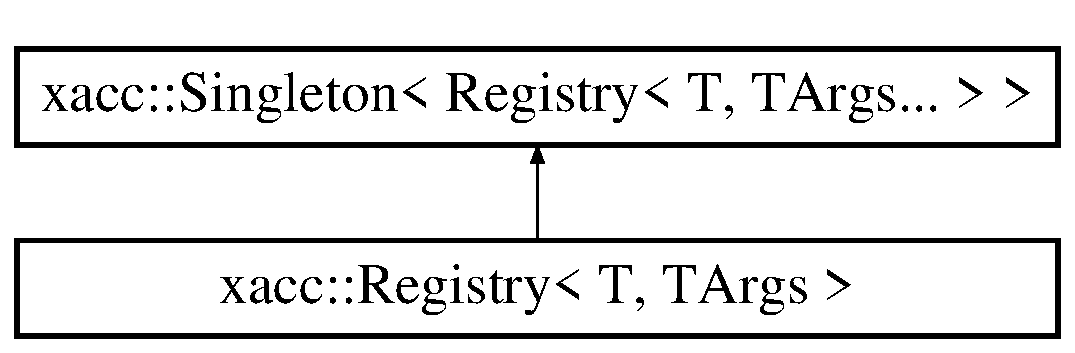
\includegraphics[height=2.000000cm]{a00070}
\end{center}
\end{figure}
\subsection*{Public Types}
\begin{DoxyCompactItemize}
\item 
using {\bfseries Creator\+Function} = std\+::function$<$ std\+::shared\+\_\+ptr$<$ T $>$(T\+Args...)$>$\hypertarget{a00070_a784134d683dee924996e12d32a6da16c}{}\label{a00070_a784134d683dee924996e12d32a6da16c}

\item 
using {\bfseries Creator\+Function\+Ptr} = std\+::shared\+\_\+ptr$<$ Creator\+Function $>$\hypertarget{a00070_a2e7d22d66dcc4644e01bcc398a3e23cc}{}\label{a00070_a2e7d22d66dcc4644e01bcc398a3e23cc}

\end{DoxyCompactItemize}
\subsection*{Public Member Functions}
\begin{DoxyCompactItemize}
\item 
bool \hyperlink{a00070_a5ec7144ddc944674313badd32452fecc}{add} (const std\+::string \&id, Creator\+Function\+Ptr f)
\item 
bool \hyperlink{a00070_a51d98b5cf6e2722655a2f597b436aa80}{add} (const std\+::string \&id, Creator\+Function\+Ptr f, std\+::shared\+\_\+ptr$<$ options\+\_\+description $>$ options)
\item 
std\+::shared\+\_\+ptr$<$ T $>$ \hyperlink{a00070_aecccbd5534276cbdd1553e43c942219b}{create} (const std\+::string \&id, T\+Args...\+args)
\item 
std\+::vector$<$ std\+::string $>$ \hyperlink{a00070_a8bff6f5c50534375abc4026662d69d2e}{get\+Registered\+Ids} ()
\item 
std\+::vector$<$ std\+::shared\+\_\+ptr$<$ options\+\_\+description $>$ $>$ {\bfseries get\+Registered\+Options} ()\hypertarget{a00070_ad1fef83142cd38d0727471c15507a0ea}{}\label{a00070_ad1fef83142cd38d0727471c15507a0ea}

\item 
std\+::size\+\_\+t \hyperlink{a00070_a2352dd7c6c85ae5c5e232b577dfa2544}{size} ()
\end{DoxyCompactItemize}
\subsection*{Protected Attributes}
\begin{DoxyCompactItemize}
\item 
std\+::map$<$ std\+::string, Creator\+Function\+Ptr $>$ \hyperlink{a00070_a7eeb7a09aafaef2012b6d0bff13c922e}{registry}
\item 
std\+::map$<$ std\+::string, std\+::shared\+\_\+ptr$<$ options\+\_\+description $>$ $>$ {\bfseries registry\+Options}\hypertarget{a00070_a790075e0e023308e5e74247fb0229a04}{}\label{a00070_a790075e0e023308e5e74247fb0229a04}

\end{DoxyCompactItemize}
\subsection*{Additional Inherited Members}


\subsection{Detailed Description}
\subsubsection*{template$<$typename T, typename... T\+Args$>$\\*
class xacc\+::\+Registry$<$ T, T\+Args $>$}

\hyperlink{a00070}{Registry} is a \hyperlink{a00081}{Singleton} that provides a mapping of string ids to creation functions that create and return the provided \hyperlink{a00070}{Registry} template parameter T.

Clients can add new creation functions to be placed in the map with a unique name key, and can request that the \hyperlink{a00070}{Registry} return a new created instance of the template parameter T. 

\subsection{Member Function Documentation}
\index{xacc\+::\+Registry@{xacc\+::\+Registry}!add@{add}}
\index{add@{add}!xacc\+::\+Registry@{xacc\+::\+Registry}}
\subsubsection[{\texorpdfstring{add(const std\+::string \&id, Creator\+Function\+Ptr f)}{add(const std::string \&id, CreatorFunctionPtr f)}}]{\setlength{\rightskip}{0pt plus 5cm}template$<$typename T, typename... T\+Args$>$ bool {\bf xacc\+::\+Registry}$<$ T, T\+Args $>$\+::add (
\begin{DoxyParamCaption}
\item[{const std\+::string \&}]{id, }
\item[{Creator\+Function\+Ptr}]{f}
\end{DoxyParamCaption}
)\hspace{0.3cm}{\ttfamily [inline]}}\hypertarget{a00070_a5ec7144ddc944674313badd32452fecc}{}\label{a00070_a5ec7144ddc944674313badd32452fecc}
Add a new creation function to the \hyperlink{a00070}{Registry}, keyed on the provided string id.


\begin{DoxyParams}{Parameters}
{\em id} & The Id of the creation function \\
\hline
{\em f} & The object\textquotesingle{}s creation function \\
\hline
\end{DoxyParams}
\begin{DoxyReturn}{Returns}
success Bool indicating if this creator was added successfully. 
\end{DoxyReturn}
\index{xacc\+::\+Registry@{xacc\+::\+Registry}!add@{add}}
\index{add@{add}!xacc\+::\+Registry@{xacc\+::\+Registry}}
\subsubsection[{\texorpdfstring{add(const std\+::string \&id, Creator\+Function\+Ptr f, std\+::shared\+\_\+ptr$<$ options\+\_\+description $>$ options)}{add(const std::string \&id, CreatorFunctionPtr f, std::shared\_ptr< options\_description > options)}}]{\setlength{\rightskip}{0pt plus 5cm}template$<$typename T, typename... T\+Args$>$ bool {\bf xacc\+::\+Registry}$<$ T, T\+Args $>$\+::add (
\begin{DoxyParamCaption}
\item[{const std\+::string \&}]{id, }
\item[{Creator\+Function\+Ptr}]{f, }
\item[{std\+::shared\+\_\+ptr$<$ options\+\_\+description $>$}]{options}
\end{DoxyParamCaption}
)\hspace{0.3cm}{\ttfamily [inline]}}\hypertarget{a00070_a51d98b5cf6e2722655a2f597b436aa80}{}\label{a00070_a51d98b5cf6e2722655a2f597b436aa80}
Add a new creation function to the \hyperlink{a00070}{Registry}, keyed on the provided string id, and related command line options for the object to be created.


\begin{DoxyParams}{Parameters}
{\em id} & The Id of the creation function \\
\hline
{\em f} & The object\textquotesingle{}s creation function \\
\hline
{\em options} & The objects command line options \\
\hline
\end{DoxyParams}
\begin{DoxyReturn}{Returns}
success Bool indicating if this creator was added successfully. 
\end{DoxyReturn}
\index{xacc\+::\+Registry@{xacc\+::\+Registry}!create@{create}}
\index{create@{create}!xacc\+::\+Registry@{xacc\+::\+Registry}}
\subsubsection[{\texorpdfstring{create(const std\+::string \&id, T\+Args...\+args)}{create(const std::string \&id, TArgs...args)}}]{\setlength{\rightskip}{0pt plus 5cm}template$<$typename T, typename... T\+Args$>$ std\+::shared\+\_\+ptr$<$T$>$ {\bf xacc\+::\+Registry}$<$ T, T\+Args $>$\+::create (
\begin{DoxyParamCaption}
\item[{const std\+::string \&}]{id, }
\item[{T\+Args...}]{args}
\end{DoxyParamCaption}
)\hspace{0.3cm}{\ttfamily [inline]}}\hypertarget{a00070_aecccbd5534276cbdd1553e43c942219b}{}\label{a00070_aecccbd5534276cbdd1553e43c942219b}
Create an instance of T by using the creation function found at the given key string id.


\begin{DoxyParams}{Parameters}
{\em id} & The Id of the creation function \\
\hline
\end{DoxyParams}
\begin{DoxyReturn}{Returns}
object Shared Pointer for the created object. 
\end{DoxyReturn}
\index{xacc\+::\+Registry@{xacc\+::\+Registry}!get\+Registered\+Ids@{get\+Registered\+Ids}}
\index{get\+Registered\+Ids@{get\+Registered\+Ids}!xacc\+::\+Registry@{xacc\+::\+Registry}}
\subsubsection[{\texorpdfstring{get\+Registered\+Ids()}{getRegisteredIds()}}]{\setlength{\rightskip}{0pt plus 5cm}template$<$typename T, typename... T\+Args$>$ std\+::vector$<$std\+::string$>$ {\bf xacc\+::\+Registry}$<$ T, T\+Args $>$\+::get\+Registered\+Ids (
\begin{DoxyParamCaption}
{}
\end{DoxyParamCaption}
)\hspace{0.3cm}{\ttfamily [inline]}}\hypertarget{a00070_a8bff6f5c50534375abc4026662d69d2e}{}\label{a00070_a8bff6f5c50534375abc4026662d69d2e}
Return the keys from the registry map.

\begin{DoxyReturn}{Returns}
ids The registered creator Ids 
\end{DoxyReturn}
\index{xacc\+::\+Registry@{xacc\+::\+Registry}!size@{size}}
\index{size@{size}!xacc\+::\+Registry@{xacc\+::\+Registry}}
\subsubsection[{\texorpdfstring{size()}{size()}}]{\setlength{\rightskip}{0pt plus 5cm}template$<$typename T, typename... T\+Args$>$ std\+::size\+\_\+t {\bf xacc\+::\+Registry}$<$ T, T\+Args $>$\+::size (
\begin{DoxyParamCaption}
{}
\end{DoxyParamCaption}
)\hspace{0.3cm}{\ttfamily [inline]}}\hypertarget{a00070_a2352dd7c6c85ae5c5e232b577dfa2544}{}\label{a00070_a2352dd7c6c85ae5c5e232b577dfa2544}
Return the number of creation functions this registry contains.

\begin{DoxyReturn}{Returns}
size The number of creators in this \hyperlink{a00070}{Registry} 
\end{DoxyReturn}


\subsection{Member Data Documentation}
\index{xacc\+::\+Registry@{xacc\+::\+Registry}!registry@{registry}}
\index{registry@{registry}!xacc\+::\+Registry@{xacc\+::\+Registry}}
\subsubsection[{\texorpdfstring{registry}{registry}}]{\setlength{\rightskip}{0pt plus 5cm}template$<$typename T, typename... T\+Args$>$ std\+::map$<$std\+::string, Creator\+Function\+Ptr$>$ {\bf xacc\+::\+Registry}$<$ T, T\+Args $>$\+::registry\hspace{0.3cm}{\ttfamily [protected]}}\hypertarget{a00070_a7eeb7a09aafaef2012b6d0bff13c922e}{}\label{a00070_a7eeb7a09aafaef2012b6d0bff13c922e}
Reference to the database of creation functions for classes of superclass type T. 

The documentation for this class was generated from the following file\+:\begin{DoxyCompactItemize}
\item 
Registry.\+hpp\end{DoxyCompactItemize}

\hypertarget{a00071}{}\section{xacc\+:\+:quantum\+:\+:Rigetti\+Accelerator Class Reference}
\label{a00071}\index{xacc\+::quantum\+::\+Rigetti\+Accelerator@{xacc\+::quantum\+::\+Rigetti\+Accelerator}}


{\ttfamily \#include $<$Rigetti\+Accelerator.\+hpp$>$}

Inheritance diagram for xacc\+:\+:quantum\+:\+:Rigetti\+Accelerator\+:\begin{figure}[H]
\begin{center}
\leavevmode
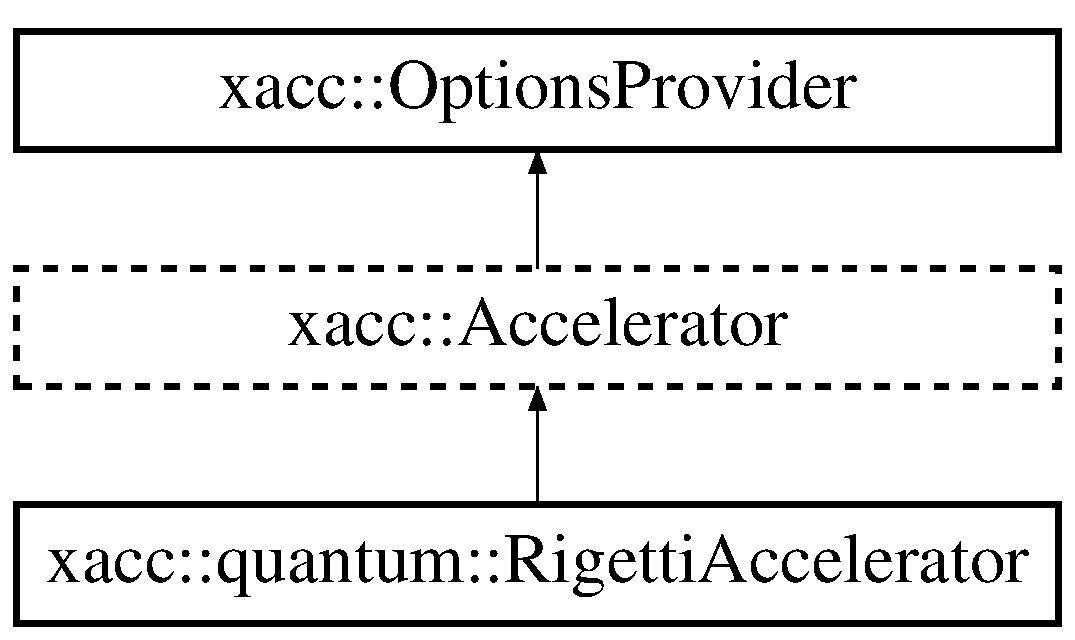
\includegraphics[height=3.000000cm]{a00071}
\end{center}
\end{figure}
\subsection*{Public Member Functions}
\begin{DoxyCompactItemize}
\item 
std\+::shared\+\_\+ptr$<$ \hyperlink{a00013}{Accelerator\+Buffer} $>$ \hyperlink{a00071_a731551c94b1abef40d2cf032e8712df6}{create\+Buffer} (const std\+::string \&var\+Id, const int size)
\item 
virtual std\+::shared\+\_\+ptr$<$ \hyperlink{a00013}{Accelerator\+Buffer} $>$ \hyperlink{a00071_ada3ceb986e51ab5aa721f2a08e083cd6}{create\+Buffer} (const std\+::string \&var\+Id)
\item 
virtual void \hyperlink{a00071_ab8b6af9bb9dcb110201e9ee5cac74b4f}{initialize} ()
\item 
virtual bool \hyperlink{a00071_a61352c07062597aad2393fbeed4cc025}{is\+Valid\+Buffer\+Size} (const int N\+Bits)
\item 
virtual void \hyperlink{a00071_afce7bbd1b0f04300a9920952e9d12ef4}{execute} (std\+::shared\+\_\+ptr$<$ \hyperlink{a00013}{Accelerator\+Buffer} $>$ buffer, const std\+::shared\+\_\+ptr$<$ \hyperlink{a00038}{xacc\+::\+Function} $>$ kernel)
\item 
virtual Accelerator\+Type \hyperlink{a00071_aab0d4674da5273d55407b9ab77cde890}{get\+Type} ()
\item 
virtual std\+::vector$<$ \hyperlink{a00051}{xacc\+::\+I\+R\+Transformation} $>$ \hyperlink{a00071_a443683a1dfb000603c640b2ee303cf66}{get\+I\+R\+Transformations} ()
\item 
virtual std\+::shared\+\_\+ptr$<$ options\+\_\+description $>$ \hyperlink{a00071_a9ee9e62aecbccf193894ca3388676f9f}{get\+Options} ()
\item 
{\bfseries Rigetti\+Accelerator} (std\+::shared\+\_\+ptr$<$ fire\+::util\+::\+I\+Networking\+Tool $>$ http)\hypertarget{a00071_aa92ba39441ec9c261fbddee23a84d6ac}{}\label{a00071_aa92ba39441ec9c261fbddee23a84d6ac}

\item 
virtual \hyperlink{a00071_a7c86895d1c29afa8b7e18476144a3fcf}{$\sim$\+Rigetti\+Accelerator} ()
\end{DoxyCompactItemize}
\subsection*{Static Public Member Functions}
\begin{DoxyCompactItemize}
\item 
static void \hyperlink{a00071_a757d25e0e7fe0f53635b97a97d74265c}{register\+Accelerator} ()
\end{DoxyCompactItemize}
\subsection*{Protected Attributes}
\begin{DoxyCompactItemize}
\item 
std\+::shared\+\_\+ptr$<$ fire\+::util\+::\+I\+Networking\+Tool $>$ {\bfseries http\+Client}\hypertarget{a00071_add34bdf35f40e3d00da366795eaa7fcb}{}\label{a00071_add34bdf35f40e3d00da366795eaa7fcb}

\end{DoxyCompactItemize}
\subsection*{Additional Inherited Members}


\subsection{Detailed Description}
The \hyperlink{a00071}{Rigetti\+Accelerator} is a Q\+P\+U\+Gate \hyperlink{a00011}{Accelerator} that provides an execute implementation that maps X\+A\+CC \hyperlink{a00050}{IR} to an equivalent Quil string, and executes it on the Rigetti superconducting quantum chip at api.\+rigetti.\+com/qvm through Fire\textquotesingle{}s H\+T\+TP Client utilities. 

\subsection{Constructor \& Destructor Documentation}
\index{xacc\+::quantum\+::\+Rigetti\+Accelerator@{xacc\+::quantum\+::\+Rigetti\+Accelerator}!````~Rigetti\+Accelerator@{$\sim$\+Rigetti\+Accelerator}}
\index{````~Rigetti\+Accelerator@{$\sim$\+Rigetti\+Accelerator}!xacc\+::quantum\+::\+Rigetti\+Accelerator@{xacc\+::quantum\+::\+Rigetti\+Accelerator}}
\subsubsection[{\texorpdfstring{$\sim$\+Rigetti\+Accelerator()}{~RigettiAccelerator()}}]{\setlength{\rightskip}{0pt plus 5cm}virtual xacc\+::quantum\+::\+Rigetti\+Accelerator\+::$\sim$\+Rigetti\+Accelerator (
\begin{DoxyParamCaption}
{}
\end{DoxyParamCaption}
)\hspace{0.3cm}{\ttfamily [inline]}, {\ttfamily [virtual]}}\hypertarget{a00071_a7c86895d1c29afa8b7e18476144a3fcf}{}\label{a00071_a7c86895d1c29afa8b7e18476144a3fcf}
The destructor 

\subsection{Member Function Documentation}
\index{xacc\+::quantum\+::\+Rigetti\+Accelerator@{xacc\+::quantum\+::\+Rigetti\+Accelerator}!create\+Buffer@{create\+Buffer}}
\index{create\+Buffer@{create\+Buffer}!xacc\+::quantum\+::\+Rigetti\+Accelerator@{xacc\+::quantum\+::\+Rigetti\+Accelerator}}
\subsubsection[{\texorpdfstring{create\+Buffer(const std\+::string \&var\+Id, const int size)}{createBuffer(const std::string \&varId, const int size)}}]{\setlength{\rightskip}{0pt plus 5cm}std\+::shared\+\_\+ptr$<$ {\bf Accelerator\+Buffer} $>$ xacc\+::quantum\+::\+Rigetti\+Accelerator\+::create\+Buffer (
\begin{DoxyParamCaption}
\item[{const std\+::string \&}]{var\+Id, }
\item[{const int}]{size}
\end{DoxyParamCaption}
)\hspace{0.3cm}{\ttfamily [virtual]}}\hypertarget{a00071_a731551c94b1abef40d2cf032e8712df6}{}\label{a00071_a731551c94b1abef40d2cf032e8712df6}
Create, store, and return an \hyperlink{a00013}{Accelerator\+Buffer} with the given variable id string and of the given number of bits. The string id serves as a unique identifier for future lookups and reuse of the \hyperlink{a00013}{Accelerator\+Buffer}.


\begin{DoxyParams}{Parameters}
{\em var\+Id} & \\
\hline
{\em size} & \\
\hline
\end{DoxyParams}
\begin{DoxyReturn}{Returns}

\end{DoxyReturn}


Implements \hyperlink{a00011_a064a2dbd58338364115c260267806945}{xacc\+::\+Accelerator}.

\index{xacc\+::quantum\+::\+Rigetti\+Accelerator@{xacc\+::quantum\+::\+Rigetti\+Accelerator}!create\+Buffer@{create\+Buffer}}
\index{create\+Buffer@{create\+Buffer}!xacc\+::quantum\+::\+Rigetti\+Accelerator@{xacc\+::quantum\+::\+Rigetti\+Accelerator}}
\subsubsection[{\texorpdfstring{create\+Buffer(const std\+::string \&var\+Id)}{createBuffer(const std::string \&varId)}}]{\setlength{\rightskip}{0pt plus 5cm}std\+::shared\+\_\+ptr$<$ {\bf Accelerator\+Buffer} $>$ xacc\+::quantum\+::\+Rigetti\+Accelerator\+::create\+Buffer (
\begin{DoxyParamCaption}
\item[{const std\+::string \&}]{var\+Id}
\end{DoxyParamCaption}
)\hspace{0.3cm}{\ttfamily [virtual]}}\hypertarget{a00071_ada3ceb986e51ab5aa721f2a08e083cd6}{}\label{a00071_ada3ceb986e51ab5aa721f2a08e083cd6}
Create, store, and return an \hyperlink{a00013}{Accelerator\+Buffer} with the given variable id string. This method returns all available qubits for this \hyperlink{a00011}{Accelerator}. The string id serves as a unique identifier for future lookups and reuse of the \hyperlink{a00013}{Accelerator\+Buffer}.


\begin{DoxyParams}{Parameters}
{\em var\+Id} & The variable name of the created buffer \\
\hline
\end{DoxyParams}
\begin{DoxyReturn}{Returns}
buffer The buffer instance created. 
\end{DoxyReturn}


Implements \hyperlink{a00011_aab5046e8d83ab390302e0f49533e95fc}{xacc\+::\+Accelerator}.

\index{xacc\+::quantum\+::\+Rigetti\+Accelerator@{xacc\+::quantum\+::\+Rigetti\+Accelerator}!execute@{execute}}
\index{execute@{execute}!xacc\+::quantum\+::\+Rigetti\+Accelerator@{xacc\+::quantum\+::\+Rigetti\+Accelerator}}
\subsubsection[{\texorpdfstring{execute(std\+::shared\+\_\+ptr$<$ Accelerator\+Buffer $>$ buffer, const std\+::shared\+\_\+ptr$<$ xacc\+::\+Function $>$ kernel)}{execute(std::shared\_ptr< AcceleratorBuffer > buffer, const std::shared\_ptr< xacc::Function > kernel)}}]{\setlength{\rightskip}{0pt plus 5cm}void xacc\+::quantum\+::\+Rigetti\+Accelerator\+::execute (
\begin{DoxyParamCaption}
\item[{std\+::shared\+\_\+ptr$<$ {\bf Accelerator\+Buffer} $>$}]{buffer, }
\item[{const std\+::shared\+\_\+ptr$<$ {\bf xacc\+::\+Function} $>$}]{kernel}
\end{DoxyParamCaption}
)\hspace{0.3cm}{\ttfamily [virtual]}}\hypertarget{a00071_afce7bbd1b0f04300a9920952e9d12ef4}{}\label{a00071_afce7bbd1b0f04300a9920952e9d12ef4}
Execute the kernel on the provided \hyperlink{a00013}{Accelerator\+Buffer} through a H\+T\+TP Post of Quil instructions to the Rigetti Q\+PU at api.\+rigetti.\+com/qvm


\begin{DoxyParams}{Parameters}
{\em ir} & \\
\hline
\end{DoxyParams}
\index{xacc\+::quantum\+::\+Rigetti\+Accelerator@{xacc\+::quantum\+::\+Rigetti\+Accelerator}!get\+I\+R\+Transformations@{get\+I\+R\+Transformations}}
\index{get\+I\+R\+Transformations@{get\+I\+R\+Transformations}!xacc\+::quantum\+::\+Rigetti\+Accelerator@{xacc\+::quantum\+::\+Rigetti\+Accelerator}}
\subsubsection[{\texorpdfstring{get\+I\+R\+Transformations()}{getIRTransformations()}}]{\setlength{\rightskip}{0pt plus 5cm}virtual std\+::vector$<${\bf xacc\+::\+I\+R\+Transformation}$>$ xacc\+::quantum\+::\+Rigetti\+Accelerator\+::get\+I\+R\+Transformations (
\begin{DoxyParamCaption}
{}
\end{DoxyParamCaption}
)\hspace{0.3cm}{\ttfamily [inline]}, {\ttfamily [virtual]}}\hypertarget{a00071_a443683a1dfb000603c640b2ee303cf66}{}\label{a00071_a443683a1dfb000603c640b2ee303cf66}
We have no need to transform the \hyperlink{a00050}{IR} for this \hyperlink{a00011}{Accelerator}, so return an empty list, for now. \begin{DoxyReturn}{Returns}

\end{DoxyReturn}


Implements \hyperlink{a00011_ad6e4a642dcb24e552675bcbeff1e1b04}{xacc\+::\+Accelerator}.

\index{xacc\+::quantum\+::\+Rigetti\+Accelerator@{xacc\+::quantum\+::\+Rigetti\+Accelerator}!get\+Options@{get\+Options}}
\index{get\+Options@{get\+Options}!xacc\+::quantum\+::\+Rigetti\+Accelerator@{xacc\+::quantum\+::\+Rigetti\+Accelerator}}
\subsubsection[{\texorpdfstring{get\+Options()}{getOptions()}}]{\setlength{\rightskip}{0pt plus 5cm}virtual std\+::shared\+\_\+ptr$<$options\+\_\+description$>$ xacc\+::quantum\+::\+Rigetti\+Accelerator\+::get\+Options (
\begin{DoxyParamCaption}
{}
\end{DoxyParamCaption}
)\hspace{0.3cm}{\ttfamily [inline]}, {\ttfamily [virtual]}}\hypertarget{a00071_a9ee9e62aecbccf193894ca3388676f9f}{}\label{a00071_a9ee9e62aecbccf193894ca3388676f9f}
Return all relevant \hyperlink{a00071}{Rigetti\+Accelerator} runtime options. Users can set the api-\/key, execution type, and number of triels from the command line with these options. 

Reimplemented from \hyperlink{a00011_a98c9eda6b54367c75667ecfbbf167979}{xacc\+::\+Accelerator}.

\index{xacc\+::quantum\+::\+Rigetti\+Accelerator@{xacc\+::quantum\+::\+Rigetti\+Accelerator}!get\+Type@{get\+Type}}
\index{get\+Type@{get\+Type}!xacc\+::quantum\+::\+Rigetti\+Accelerator@{xacc\+::quantum\+::\+Rigetti\+Accelerator}}
\subsubsection[{\texorpdfstring{get\+Type()}{getType()}}]{\setlength{\rightskip}{0pt plus 5cm}virtual Accelerator\+Type xacc\+::quantum\+::\+Rigetti\+Accelerator\+::get\+Type (
\begin{DoxyParamCaption}
{}
\end{DoxyParamCaption}
)\hspace{0.3cm}{\ttfamily [inline]}, {\ttfamily [virtual]}}\hypertarget{a00071_aab0d4674da5273d55407b9ab77cde890}{}\label{a00071_aab0d4674da5273d55407b9ab77cde890}
This \hyperlink{a00011}{Accelerator} models Q\+PU Gate accelerators. \begin{DoxyReturn}{Returns}

\end{DoxyReturn}


Implements \hyperlink{a00011_aaffc3e4bb9880eb5041b1b58ee4c2665}{xacc\+::\+Accelerator}.

\index{xacc\+::quantum\+::\+Rigetti\+Accelerator@{xacc\+::quantum\+::\+Rigetti\+Accelerator}!initialize@{initialize}}
\index{initialize@{initialize}!xacc\+::quantum\+::\+Rigetti\+Accelerator@{xacc\+::quantum\+::\+Rigetti\+Accelerator}}
\subsubsection[{\texorpdfstring{initialize()}{initialize()}}]{\setlength{\rightskip}{0pt plus 5cm}virtual void xacc\+::quantum\+::\+Rigetti\+Accelerator\+::initialize (
\begin{DoxyParamCaption}
{}
\end{DoxyParamCaption}
)\hspace{0.3cm}{\ttfamily [inline]}, {\ttfamily [virtual]}}\hypertarget{a00071_ab8b6af9bb9dcb110201e9ee5cac74b4f}{}\label{a00071_ab8b6af9bb9dcb110201e9ee5cac74b4f}
Initialize this \hyperlink{a00011}{Accelerator}. This method is called by the X\+A\+CC framework after an \hyperlink{a00011}{Accelerator} has been requested and created. Perform any work you need done before execution here. 

Implements \hyperlink{a00011_a8cdc6f0c5a660013c29c07657a06303b}{xacc\+::\+Accelerator}.

\index{xacc\+::quantum\+::\+Rigetti\+Accelerator@{xacc\+::quantum\+::\+Rigetti\+Accelerator}!is\+Valid\+Buffer\+Size@{is\+Valid\+Buffer\+Size}}
\index{is\+Valid\+Buffer\+Size@{is\+Valid\+Buffer\+Size}!xacc\+::quantum\+::\+Rigetti\+Accelerator@{xacc\+::quantum\+::\+Rigetti\+Accelerator}}
\subsubsection[{\texorpdfstring{is\+Valid\+Buffer\+Size(const int N\+Bits)}{isValidBufferSize(const int NBits)}}]{\setlength{\rightskip}{0pt plus 5cm}bool xacc\+::quantum\+::\+Rigetti\+Accelerator\+::is\+Valid\+Buffer\+Size (
\begin{DoxyParamCaption}
\item[{const int}]{N\+Bits}
\end{DoxyParamCaption}
)\hspace{0.3cm}{\ttfamily [virtual]}}\hypertarget{a00071_a61352c07062597aad2393fbeed4cc025}{}\label{a00071_a61352c07062597aad2393fbeed4cc025}
Return true if this \hyperlink{a00011}{Accelerator} can allocated N\+Bits number of bits. 
\begin{DoxyParams}{Parameters}
{\em N\+Bits} & \\
\hline
\end{DoxyParams}
\begin{DoxyReturn}{Returns}

\end{DoxyReturn}


Implements \hyperlink{a00011_ae51584850faeec77299058383977ddeb}{xacc\+::\+Accelerator}.

\index{xacc\+::quantum\+::\+Rigetti\+Accelerator@{xacc\+::quantum\+::\+Rigetti\+Accelerator}!register\+Accelerator@{register\+Accelerator}}
\index{register\+Accelerator@{register\+Accelerator}!xacc\+::quantum\+::\+Rigetti\+Accelerator@{xacc\+::quantum\+::\+Rigetti\+Accelerator}}
\subsubsection[{\texorpdfstring{register\+Accelerator()}{registerAccelerator()}}]{\setlength{\rightskip}{0pt plus 5cm}static void xacc\+::quantum\+::\+Rigetti\+Accelerator\+::register\+Accelerator (
\begin{DoxyParamCaption}
{}
\end{DoxyParamCaption}
)\hspace{0.3cm}{\ttfamily [inline]}, {\ttfamily [static]}}\hypertarget{a00071_a757d25e0e7fe0f53635b97a97d74265c}{}\label{a00071_a757d25e0e7fe0f53635b97a97d74265c}
Register this \hyperlink{a00011}{Accelerator} with the framework. 

The documentation for this class was generated from the following files\+:\begin{DoxyCompactItemize}
\item 
Rigetti\+Accelerator.\+hpp\item 
Rigetti\+Accelerator.\+cpp\end{DoxyCompactItemize}

\hypertarget{a00072}{}\section{xacc\+:\+:Runtime\+Options Class Reference}
\label{a00072}\index{xacc\+::\+Runtime\+Options@{xacc\+::\+Runtime\+Options}}


{\ttfamily \#include $<$Runtime\+Options.\+hpp$>$}

Inheritance diagram for xacc\+:\+:Runtime\+Options\+:\begin{figure}[H]
\begin{center}
\leavevmode
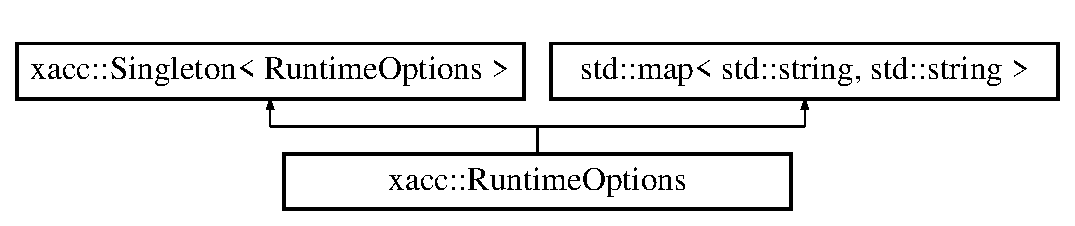
\includegraphics[height=2.000000cm]{a00072}
\end{center}
\end{figure}
\subsection*{Public Member Functions}
\begin{DoxyCompactItemize}
\item 
bool \hyperlink{a00072_a3603aecb87461efedd0fabbef966c80c}{exists} (const std\+::string \&key)
\end{DoxyCompactItemize}
\subsection*{Additional Inherited Members}


\subsection{Detailed Description}
The \hyperlink{a00072}{Runtime\+Options} class is a \hyperlink{a00081}{Singleton} mapping of string keys to string values. It is used throughout X\+A\+CC to provide and share runtime options that are provided from X\+A\+CC users via the command line. 

\subsection{Member Function Documentation}
\index{xacc\+::\+Runtime\+Options@{xacc\+::\+Runtime\+Options}!exists@{exists}}
\index{exists@{exists}!xacc\+::\+Runtime\+Options@{xacc\+::\+Runtime\+Options}}
\subsubsection[{\texorpdfstring{exists(const std\+::string \&key)}{exists(const std::string \&key)}}]{\setlength{\rightskip}{0pt plus 5cm}bool xacc\+::\+Runtime\+Options\+::exists (
\begin{DoxyParamCaption}
\item[{const std\+::string \&}]{key}
\end{DoxyParamCaption}
)\hspace{0.3cm}{\ttfamily [inline]}}\hypertarget{a00072_a3603aecb87461efedd0fabbef966c80c}{}\label{a00072_a3603aecb87461efedd0fabbef966c80c}
Convenience method to get whether the give key exists in the \hyperlink{a00072}{Runtime\+Options}.


\begin{DoxyParams}{Parameters}
{\em key} & The key to check exists \\
\hline
\end{DoxyParams}


The documentation for this class was generated from the following file\+:\begin{DoxyCompactItemize}
\item 
Runtime\+Options.\+hpp\end{DoxyCompactItemize}

\hypertarget{a00073}{}\section{xacc\+:\+:quantum\+:\+:Rx Class Reference}
\label{a00073}\index{xacc\+::quantum\+::\+Rx@{xacc\+::quantum\+::\+Rx}}
Inheritance diagram for xacc\+:\+:quantum\+:\+:Rx\+:\begin{figure}[H]
\begin{center}
\leavevmode
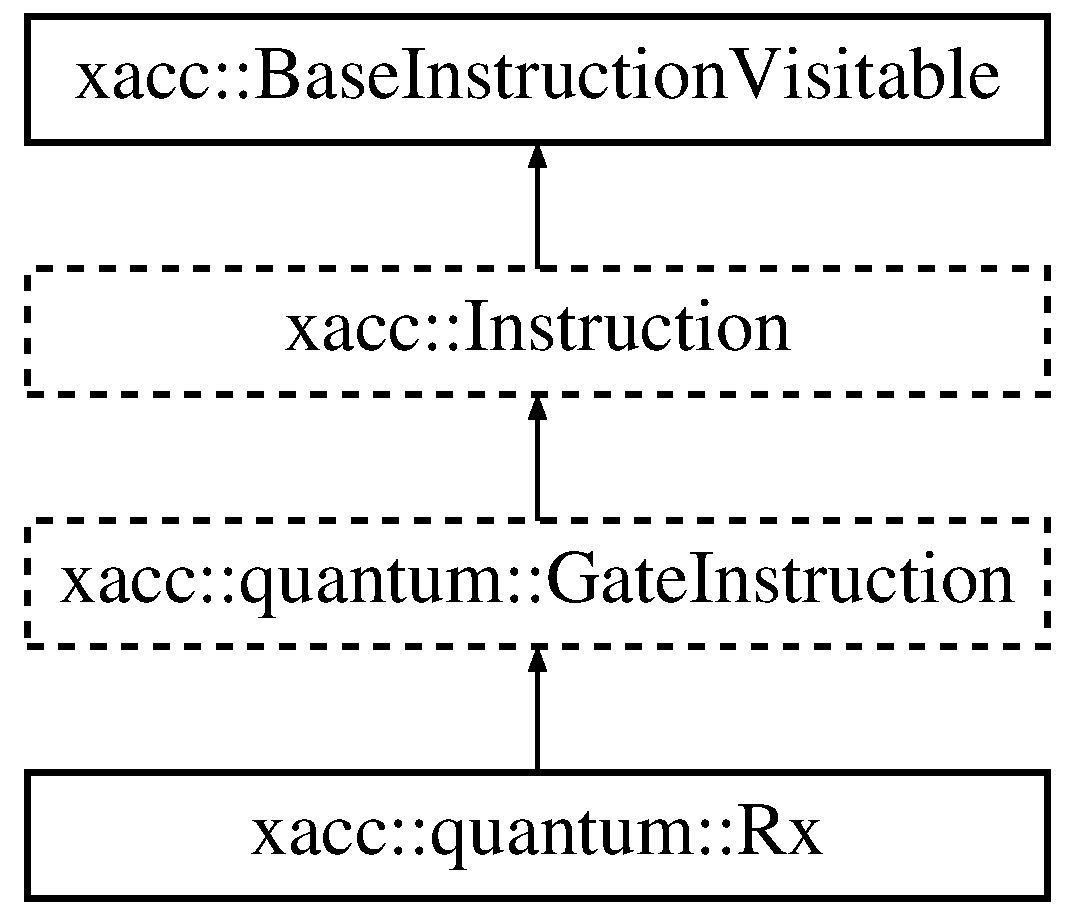
\includegraphics[height=4.000000cm]{a00073}
\end{center}
\end{figure}
\subsection*{Public Member Functions}
\begin{DoxyCompactItemize}
\item 
{\bfseries Rx} (std\+::vector$<$ int $>$ \hyperlink{a00041_a2a56be6c2519ea65df4d06f4abae1393}{qbits})\hypertarget{a00073_a03babfe938a6cbf7f744fcd31a52d92d}{}\label{a00073_a03babfe938a6cbf7f744fcd31a52d92d}

\item 
{\bfseries Rx} (int qbit, double theta)\hypertarget{a00073_a01667b11d34d5621b98ebff9a07d9bbf}{}\label{a00073_a01667b11d34d5621b98ebff9a07d9bbf}

\end{DoxyCompactItemize}
\subsection*{Additional Inherited Members}


The documentation for this class was generated from the following files\+:\begin{DoxyCompactItemize}
\item 
Rx.\+hpp\item 
Rx.\+cpp\end{DoxyCompactItemize}

\hypertarget{a00074}{}\section{xacc\+:\+:quantum\+:\+:Ry Class Reference}
\label{a00074}\index{xacc\+::quantum\+::\+Ry@{xacc\+::quantum\+::\+Ry}}
Inheritance diagram for xacc\+:\+:quantum\+:\+:Ry\+:\begin{figure}[H]
\begin{center}
\leavevmode
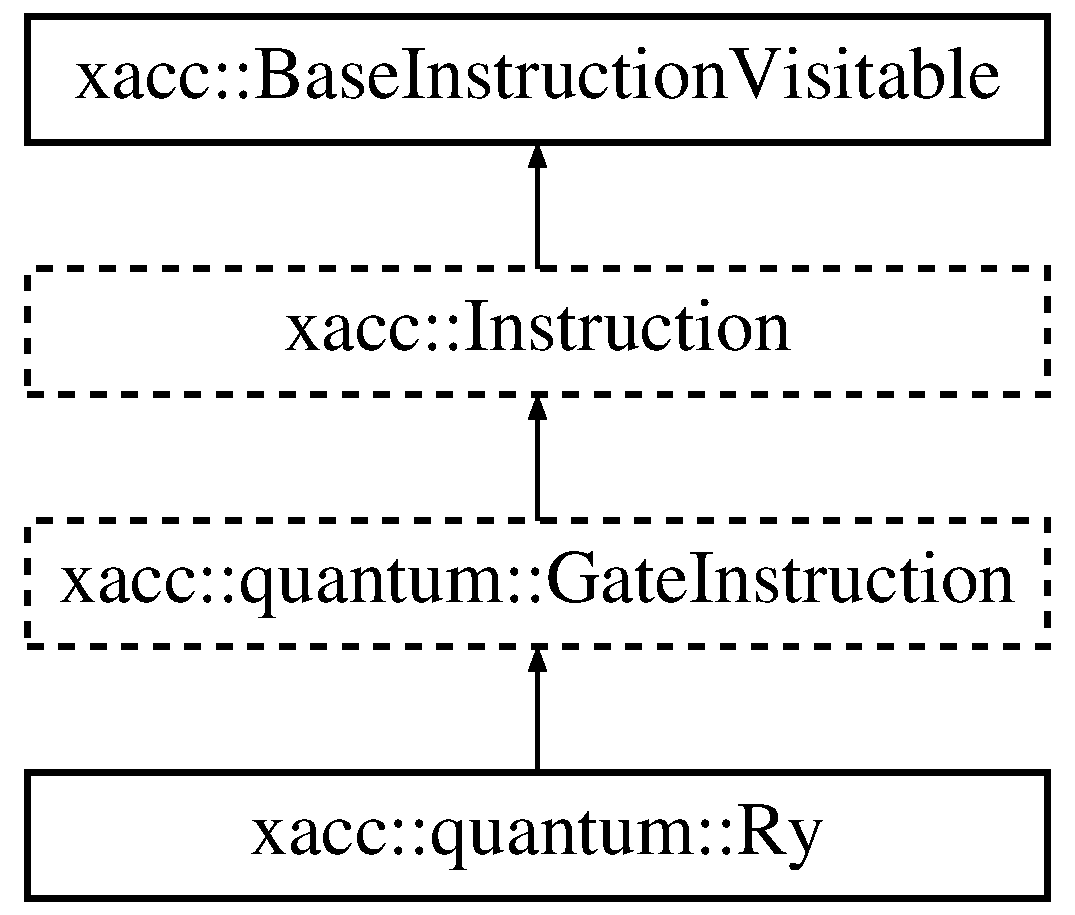
\includegraphics[height=4.000000cm]{a00074}
\end{center}
\end{figure}
\subsection*{Public Member Functions}
\begin{DoxyCompactItemize}
\item 
{\bfseries Ry} (std\+::vector$<$ int $>$ \hyperlink{a00041_a2a56be6c2519ea65df4d06f4abae1393}{qbits})\hypertarget{a00074_a542e1c0576a8e784f6cece4c77598486}{}\label{a00074_a542e1c0576a8e784f6cece4c77598486}

\item 
{\bfseries Ry} (int qbit, double theta)\hypertarget{a00074_a1cb81fe622168ba8d79fa2a78b5b0006}{}\label{a00074_a1cb81fe622168ba8d79fa2a78b5b0006}

\end{DoxyCompactItemize}
\subsection*{Additional Inherited Members}


The documentation for this class was generated from the following files\+:\begin{DoxyCompactItemize}
\item 
Ry.\+hpp\item 
Ry.\+cpp\end{DoxyCompactItemize}

\hypertarget{a00075}{}\section{xacc\+:\+:quantum\+:\+:Rz Class Reference}
\label{a00075}\index{xacc\+::quantum\+::\+Rz@{xacc\+::quantum\+::\+Rz}}
Inheritance diagram for xacc\+:\+:quantum\+:\+:Rz\+:\begin{figure}[H]
\begin{center}
\leavevmode
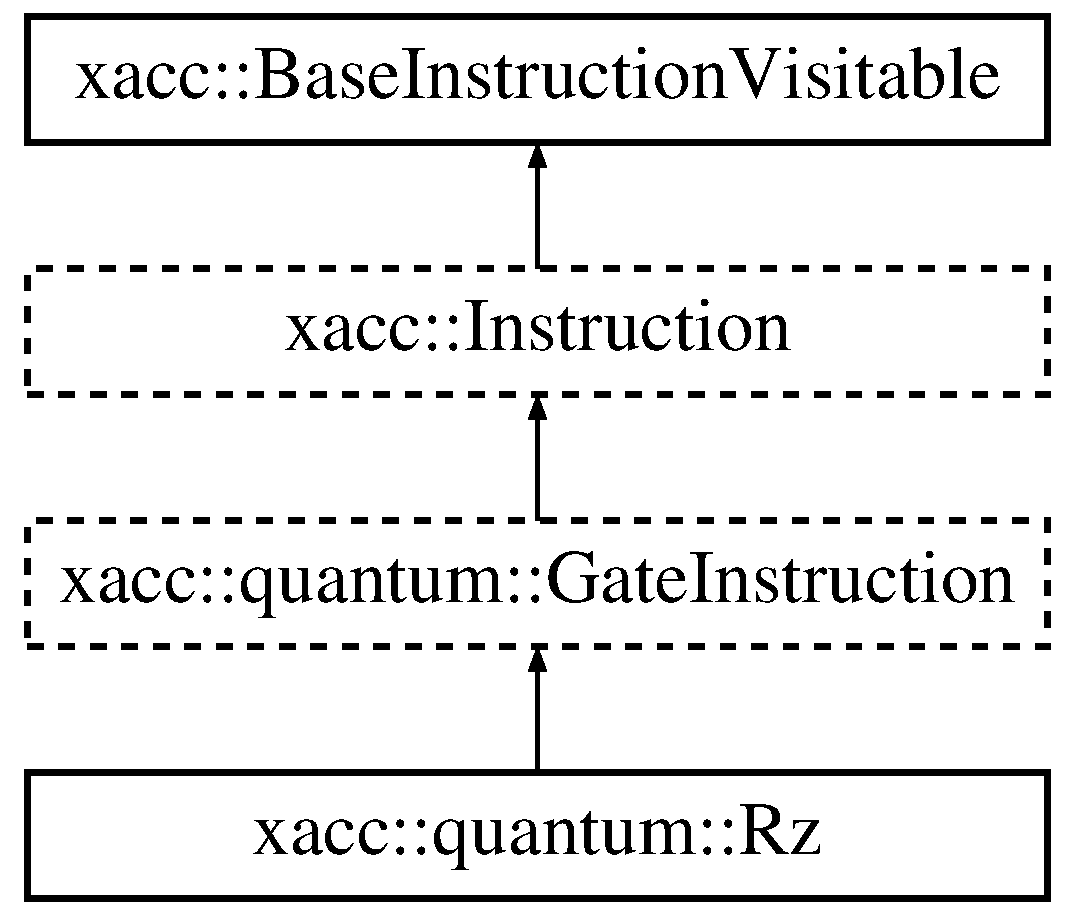
\includegraphics[height=4.000000cm]{a00075}
\end{center}
\end{figure}
\subsection*{Public Member Functions}
\begin{DoxyCompactItemize}
\item 
{\bfseries Rz} (std\+::vector$<$ int $>$ \hyperlink{a00041_a2a56be6c2519ea65df4d06f4abae1393}{qbits})\hypertarget{a00075_a7ce912c7f9c9e8f4e7e60f9dba95538b}{}\label{a00075_a7ce912c7f9c9e8f4e7e60f9dba95538b}

\item 
{\bfseries Rz} (int qbit, double theta)\hypertarget{a00075_ae30eaf75feb8f896c22043629d21b834}{}\label{a00075_ae30eaf75feb8f896c22043629d21b834}

\end{DoxyCompactItemize}
\subsection*{Additional Inherited Members}


The documentation for this class was generated from the following files\+:\begin{DoxyCompactItemize}
\item 
Rz.\+hpp\item 
Rz.\+cpp\end{DoxyCompactItemize}

\hypertarget{a00076}{}\section{xacc\+:\+:quantum\+:\+:Scaffold\+A\+S\+T\+Consumer Class Reference}
\label{a00076}\index{xacc\+::quantum\+::\+Scaffold\+A\+S\+T\+Consumer@{xacc\+::quantum\+::\+Scaffold\+A\+S\+T\+Consumer}}
Inheritance diagram for xacc\+:\+:quantum\+:\+:Scaffold\+A\+S\+T\+Consumer\+:\begin{figure}[H]
\begin{center}
\leavevmode
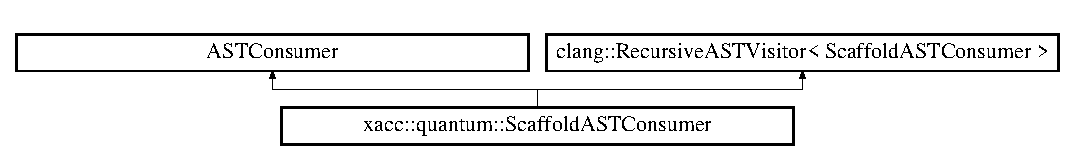
\includegraphics[height=1.717791cm]{a00076}
\end{center}
\end{figure}
\subsection*{Public Member Functions}
\begin{DoxyCompactItemize}
\item 
virtual bool {\bfseries Handle\+Top\+Level\+Decl} (Decl\+Group\+Ref DR)\hypertarget{a00076_ae846fd40684f3a1f820b8711e1204089}{}\label{a00076_ae846fd40684f3a1f820b8711e1204089}

\item 
bool {\bfseries Visit\+Stmt} (clang\+::\+Stmt $\ast$s)\hypertarget{a00076_a6693c27f68332d8142fbdcb405e3259b}{}\label{a00076_a6693c27f68332d8142fbdcb405e3259b}

\item 
bool {\bfseries Visit\+Decl} (clang\+::\+Decl $\ast$d)\hypertarget{a00076_ae6a05fe567cd8ea15feb694dbb898c33}{}\label{a00076_ae6a05fe567cd8ea15feb694dbb898c33}

\item 
bool {\bfseries Visit\+Call\+Expr} (Call\+Expr $\ast$c)\hypertarget{a00076_a1478fc9e887b04d2ad2aa8347ef6bbcb}{}\label{a00076_a1478fc9e887b04d2ad2aa8347ef6bbcb}

\item 
bool {\bfseries Visit\+Binary\+Operator} (Binary\+Operator $\ast$b)\hypertarget{a00076_a3f2f070888678caf53e57041b4f5ddd6}{}\label{a00076_a3f2f070888678caf53e57041b4f5ddd6}

\item 
std\+::shared\+\_\+ptr$<$ \hyperlink{a00050}{xacc\+::\+IR} $>$ {\bfseries get\+IR} ()\hypertarget{a00076_af9dbfa7c52b8a7de99132257e154e29a}{}\label{a00076_af9dbfa7c52b8a7de99132257e154e29a}

\item 
const std\+::string {\bfseries get\+Qubit\+Variable\+Name} ()\hypertarget{a00076_aa301f0bcae6fb5a1c17557ba08144cb4}{}\label{a00076_aa301f0bcae6fb5a1c17557ba08144cb4}

\end{DoxyCompactItemize}
\subsection*{Protected Attributes}
\begin{DoxyCompactItemize}
\item 
std\+::string {\bfseries cbit\+Var\+Name}\hypertarget{a00076_a62efc9fb3166e7f9d0a7ccb71dc5eb59}{}\label{a00076_a62efc9fb3166e7f9d0a7ccb71dc5eb59}

\item 
std\+::string {\bfseries qbit\+Var\+Name}\hypertarget{a00076_aaa908356dd67cb918d7cc913783760f9}{}\label{a00076_aaa908356dd67cb918d7cc913783760f9}

\item 
std\+::shared\+\_\+ptr$<$ \hyperlink{a00042}{xacc\+::quantum\+::\+Gate\+Q\+IR} $>$ {\bfseries ir}\hypertarget{a00076_addb230351a9ceaeb55496adc57f2b748}{}\label{a00076_addb230351a9ceaeb55496adc57f2b748}

\item 
std\+::shared\+\_\+ptr$<$ \hyperlink{a00040}{xacc\+::quantum\+::\+Gate\+Function} $>$ {\bfseries function}\hypertarget{a00076_a78d4c0227cf55778cb05f2262357c3a9}{}\label{a00076_a78d4c0227cf55778cb05f2262357c3a9}

\item 
std\+::shared\+\_\+ptr$<$ \hyperlink{a00025}{xacc\+::quantum\+::\+Conditional\+Function} $>$ {\bfseries current\+Conditional}\hypertarget{a00076_a481378bd7158942633a555500871b363}{}\label{a00076_a481378bd7158942633a555500871b363}

\item 
int {\bfseries n\+Call\+Expr\+To\+Skip} = 0\hypertarget{a00076_a3be085dc66ddcf3f6e0530a17b26e66a}{}\label{a00076_a3be085dc66ddcf3f6e0530a17b26e66a}

\item 
std\+::map$<$ std\+::string, int $>$ {\bfseries cbit\+Reg\+To\+Measured\+Qubit}\hypertarget{a00076_a6675849cfdd92413a688c6999dda40a8}{}\label{a00076_a6675849cfdd92413a688c6999dda40a8}

\end{DoxyCompactItemize}


The documentation for this class was generated from the following file\+:\begin{DoxyCompactItemize}
\item 
Scaffold\+A\+S\+T\+Consumer.\+hpp\end{DoxyCompactItemize}

\hypertarget{a00077}{}\section{xacc\+:\+:quantum\+:\+:Scaffold\+Compiler Class Reference}
\label{a00077}\index{xacc\+::quantum\+::\+Scaffold\+Compiler@{xacc\+::quantum\+::\+Scaffold\+Compiler}}


{\ttfamily \#include $<$Scaffold\+Compiler.\+hpp$>$}

Inheritance diagram for xacc\+:\+:quantum\+:\+:Scaffold\+Compiler\+:\begin{figure}[H]
\begin{center}
\leavevmode
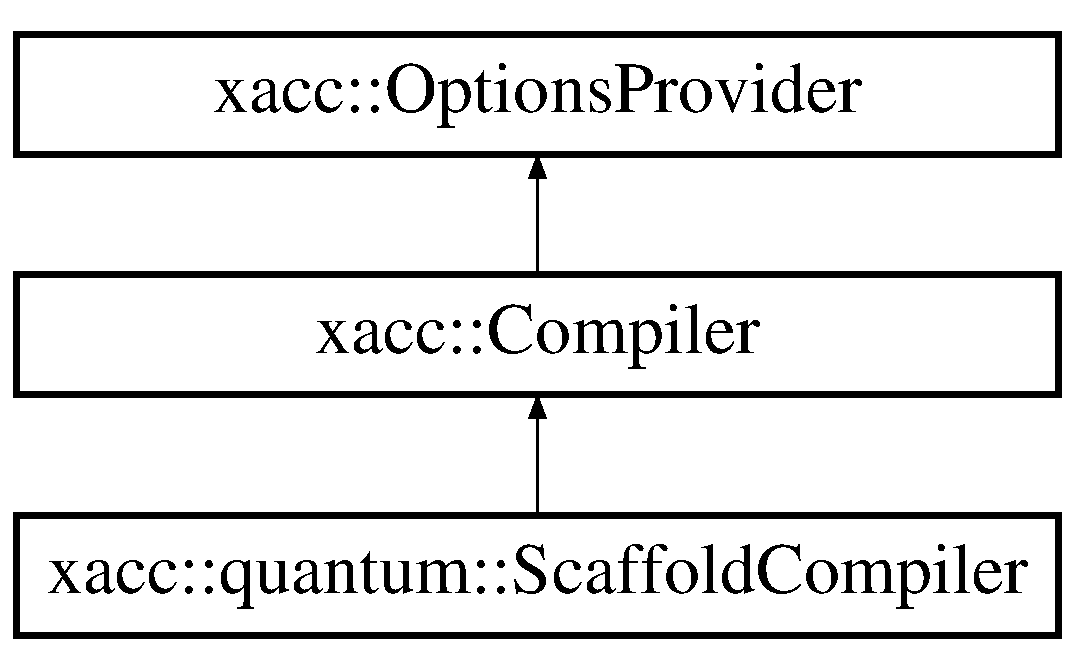
\includegraphics[height=3.000000cm]{a00077}
\end{center}
\end{figure}
\subsection*{Public Member Functions}
\begin{DoxyCompactItemize}
\item 
virtual std\+::shared\+\_\+ptr$<$ \hyperlink{a00050}{xacc\+::\+IR} $>$ \hyperlink{a00077_a7caede75bb2304ba405966651b115543}{compile} (const std\+::string \&src, std\+::shared\+\_\+ptr$<$ \hyperlink{a00011}{Accelerator} $>$ acc)
\item 
virtual std\+::shared\+\_\+ptr$<$ \hyperlink{a00050}{xacc\+::\+IR} $>$ \hyperlink{a00077_a3736ecc229fe6acdd4c991e85d7a1f08}{compile} (const std\+::string \&src)
\item 
virtual const std\+::string \hyperlink{a00077_ac7ca2941e987ba579c6f50cfbd7fb0dc}{translate} (const std\+::string \&buffer\+Variable, std\+::shared\+\_\+ptr$<$ \hyperlink{a00038}{Function} $>$ function)
\item 
virtual const std\+::string \hyperlink{a00077_a3f537054a3924a1d14f4ceb0f0181161}{get\+Name} ()
\item 
virtual \hyperlink{a00077_afb26398b07377ab9ddebc43a9376a6dd}{$\sim$\+Scaffold\+Compiler} ()
\end{DoxyCompactItemize}
\subsection*{Static Public Member Functions}
\begin{DoxyCompactItemize}
\item 
static void \hyperlink{a00077_aed16dda1e919e5af6de9953a656f62ce}{register\+Compiler} ()
\end{DoxyCompactItemize}
\subsection*{Protected Attributes}
\begin{DoxyCompactItemize}
\item 
std\+::shared\+\_\+ptr$<$ clang\+::\+Compiler\+Instance $>$ \hyperlink{a00077_af7a3a73eaab025a0ea72cc9335d8fbb4}{CI}
\item 
std\+::shared\+\_\+ptr$<$ \hyperlink{a00076}{Scaffold\+A\+S\+T\+Consumer} $>$ \hyperlink{a00077_ab1c4d36e58b97de50208e74a92d8ceb1}{consumer}
\end{DoxyCompactItemize}


\subsection{Detailed Description}
The Scaffold compiler is a subclass of the X\+A\+CC \hyperlink{a00023}{Compiler} that implements the \hyperlink{a00077_a7caede75bb2304ba405966651b115543}{compile()} and modify\+Source() methods to handle generation of quantum assembly language (or Q\+A\+SM) using an installed Scaffold compiler. 

\subsection{Constructor \& Destructor Documentation}
\index{xacc\+::quantum\+::\+Scaffold\+Compiler@{xacc\+::quantum\+::\+Scaffold\+Compiler}!````~Scaffold\+Compiler@{$\sim$\+Scaffold\+Compiler}}
\index{````~Scaffold\+Compiler@{$\sim$\+Scaffold\+Compiler}!xacc\+::quantum\+::\+Scaffold\+Compiler@{xacc\+::quantum\+::\+Scaffold\+Compiler}}
\subsubsection[{\texorpdfstring{$\sim$\+Scaffold\+Compiler()}{~ScaffoldCompiler()}}]{\setlength{\rightskip}{0pt plus 5cm}virtual xacc\+::quantum\+::\+Scaffold\+Compiler\+::$\sim$\+Scaffold\+Compiler (
\begin{DoxyParamCaption}
{}
\end{DoxyParamCaption}
)\hspace{0.3cm}{\ttfamily [inline]}, {\ttfamily [virtual]}}\hypertarget{a00077_afb26398b07377ab9ddebc43a9376a6dd}{}\label{a00077_afb26398b07377ab9ddebc43a9376a6dd}
The destructor 

\subsection{Member Function Documentation}
\index{xacc\+::quantum\+::\+Scaffold\+Compiler@{xacc\+::quantum\+::\+Scaffold\+Compiler}!compile@{compile}}
\index{compile@{compile}!xacc\+::quantum\+::\+Scaffold\+Compiler@{xacc\+::quantum\+::\+Scaffold\+Compiler}}
\subsubsection[{\texorpdfstring{compile(const std\+::string \&src, std\+::shared\+\_\+ptr$<$ Accelerator $>$ acc)}{compile(const std::string \&src, std::shared\_ptr< Accelerator > acc)}}]{\setlength{\rightskip}{0pt plus 5cm}std\+::shared\+\_\+ptr$<$ {\bf IR} $>$ xacc\+::quantum\+::\+Scaffold\+Compiler\+::compile (
\begin{DoxyParamCaption}
\item[{const std\+::string \&}]{src, }
\item[{std\+::shared\+\_\+ptr$<$ {\bf Accelerator} $>$}]{acc}
\end{DoxyParamCaption}
)\hspace{0.3cm}{\ttfamily [virtual]}}\hypertarget{a00077_a7caede75bb2304ba405966651b115543}{}\label{a00077_a7caede75bb2304ba405966651b115543}
Execute the Scaffold compiler to generate an X\+A\+CC intermediate representation instance. \begin{DoxyReturn}{Returns}
ir X\+A\+CC intermediate representation 
\end{DoxyReturn}


Implements \hyperlink{a00023_a546a40c95bb93af6a0c0ac48dbeaffc8}{xacc\+::\+Compiler}.

\index{xacc\+::quantum\+::\+Scaffold\+Compiler@{xacc\+::quantum\+::\+Scaffold\+Compiler}!compile@{compile}}
\index{compile@{compile}!xacc\+::quantum\+::\+Scaffold\+Compiler@{xacc\+::quantum\+::\+Scaffold\+Compiler}}
\subsubsection[{\texorpdfstring{compile(const std\+::string \&src)}{compile(const std::string \&src)}}]{\setlength{\rightskip}{0pt plus 5cm}std\+::shared\+\_\+ptr$<$ {\bf IR} $>$ xacc\+::quantum\+::\+Scaffold\+Compiler\+::compile (
\begin{DoxyParamCaption}
\item[{const std\+::string \&}]{src}
\end{DoxyParamCaption}
)\hspace{0.3cm}{\ttfamily [virtual]}}\hypertarget{a00077_a3736ecc229fe6acdd4c991e85d7a1f08}{}\label{a00077_a3736ecc229fe6acdd4c991e85d7a1f08}

\begin{DoxyParams}{Parameters}
{\em src} & \\
\hline
\end{DoxyParams}
\begin{DoxyReturn}{Returns}

\end{DoxyReturn}


Implements \hyperlink{a00023_a9092f5f779b570c91569b59621280c04}{xacc\+::\+Compiler}.

\index{xacc\+::quantum\+::\+Scaffold\+Compiler@{xacc\+::quantum\+::\+Scaffold\+Compiler}!get\+Name@{get\+Name}}
\index{get\+Name@{get\+Name}!xacc\+::quantum\+::\+Scaffold\+Compiler@{xacc\+::quantum\+::\+Scaffold\+Compiler}}
\subsubsection[{\texorpdfstring{get\+Name()}{getName()}}]{\setlength{\rightskip}{0pt plus 5cm}virtual const std\+::string xacc\+::quantum\+::\+Scaffold\+Compiler\+::get\+Name (
\begin{DoxyParamCaption}
{}
\end{DoxyParamCaption}
)\hspace{0.3cm}{\ttfamily [inline]}, {\ttfamily [virtual]}}\hypertarget{a00077_a3f537054a3924a1d14f4ceb0f0181161}{}\label{a00077_a3f537054a3924a1d14f4ceb0f0181161}
Return the name of this \hyperlink{a00023}{Compiler} \begin{DoxyReturn}{Returns}
name \hyperlink{a00023}{Compiler} name 
\end{DoxyReturn}


Implements \hyperlink{a00023_a87fca9100e6462122f5b687c3a0fb3fb}{xacc\+::\+Compiler}.

\index{xacc\+::quantum\+::\+Scaffold\+Compiler@{xacc\+::quantum\+::\+Scaffold\+Compiler}!register\+Compiler@{register\+Compiler}}
\index{register\+Compiler@{register\+Compiler}!xacc\+::quantum\+::\+Scaffold\+Compiler@{xacc\+::quantum\+::\+Scaffold\+Compiler}}
\subsubsection[{\texorpdfstring{register\+Compiler()}{registerCompiler()}}]{\setlength{\rightskip}{0pt plus 5cm}static void xacc\+::quantum\+::\+Scaffold\+Compiler\+::register\+Compiler (
\begin{DoxyParamCaption}
{}
\end{DoxyParamCaption}
)\hspace{0.3cm}{\ttfamily [inline]}, {\ttfamily [static]}}\hypertarget{a00077_aed16dda1e919e5af6de9953a656f62ce}{}\label{a00077_aed16dda1e919e5af6de9953a656f62ce}
Register this \hyperlink{a00023}{Compiler} with the framework. \index{xacc\+::quantum\+::\+Scaffold\+Compiler@{xacc\+::quantum\+::\+Scaffold\+Compiler}!translate@{translate}}
\index{translate@{translate}!xacc\+::quantum\+::\+Scaffold\+Compiler@{xacc\+::quantum\+::\+Scaffold\+Compiler}}
\subsubsection[{\texorpdfstring{translate(const std\+::string \&buffer\+Variable, std\+::shared\+\_\+ptr$<$ Function $>$ function)}{translate(const std::string \&bufferVariable, std::shared\_ptr< Function > function)}}]{\setlength{\rightskip}{0pt plus 5cm}const std\+::string xacc\+::quantum\+::\+Scaffold\+Compiler\+::translate (
\begin{DoxyParamCaption}
\item[{const std\+::string \&}]{buffer\+Variable, }
\item[{std\+::shared\+\_\+ptr$<$ {\bf Function} $>$}]{function}
\end{DoxyParamCaption}
)\hspace{0.3cm}{\ttfamily [virtual]}}\hypertarget{a00077_ac7ca2941e987ba579c6f50cfbd7fb0dc}{}\label{a00077_ac7ca2941e987ba579c6f50cfbd7fb0dc}
This produces a Scaffold source code representation of the given \hyperlink{a00050}{IR} \hyperlink{a00038}{Function}


\begin{DoxyParams}{Parameters}
{\em function} & The X\+A\+CC \hyperlink{a00050}{IR} \hyperlink{a00038}{Function} to translate \\
\hline
\end{DoxyParams}
\begin{DoxyReturn}{Returns}
src The source code as a string 
\end{DoxyReturn}


Implements \hyperlink{a00023_aeedbe58a33fed29e4d7694ae743e25e7}{xacc\+::\+Compiler}.



\subsection{Member Data Documentation}
\index{xacc\+::quantum\+::\+Scaffold\+Compiler@{xacc\+::quantum\+::\+Scaffold\+Compiler}!CI@{CI}}
\index{CI@{CI}!xacc\+::quantum\+::\+Scaffold\+Compiler@{xacc\+::quantum\+::\+Scaffold\+Compiler}}
\subsubsection[{\texorpdfstring{CI}{CI}}]{\setlength{\rightskip}{0pt plus 5cm}std\+::shared\+\_\+ptr$<$clang\+::\+Compiler\+Instance$>$ xacc\+::quantum\+::\+Scaffold\+Compiler\+::\+CI\hspace{0.3cm}{\ttfamily [protected]}}\hypertarget{a00077_af7a3a73eaab025a0ea72cc9335d8fbb4}{}\label{a00077_af7a3a73eaab025a0ea72cc9335d8fbb4}
Reference to the Scaffold Clang \hyperlink{a00023}{Compiler} \index{xacc\+::quantum\+::\+Scaffold\+Compiler@{xacc\+::quantum\+::\+Scaffold\+Compiler}!consumer@{consumer}}
\index{consumer@{consumer}!xacc\+::quantum\+::\+Scaffold\+Compiler@{xacc\+::quantum\+::\+Scaffold\+Compiler}}
\subsubsection[{\texorpdfstring{consumer}{consumer}}]{\setlength{\rightskip}{0pt plus 5cm}std\+::shared\+\_\+ptr$<${\bf Scaffold\+A\+S\+T\+Consumer}$>$ xacc\+::quantum\+::\+Scaffold\+Compiler\+::consumer\hspace{0.3cm}{\ttfamily [protected]}}\hypertarget{a00077_ab1c4d36e58b97de50208e74a92d8ceb1}{}\label{a00077_ab1c4d36e58b97de50208e74a92d8ceb1}
Reference to our A\+ST Consumer, this gives us the compiled \hyperlink{a00050}{IR} \hyperlink{a00038}{Function} and the Qubit Variable Name 

The documentation for this class was generated from the following files\+:\begin{DoxyCompactItemize}
\item 
Scaffold\+Compiler.\+hpp\item 
Scaffold\+Compiler.\+cpp\end{DoxyCompactItemize}

\hypertarget{a00078}{}\section{xacc\+:\+:quantum\+:\+:Scaffold\+I\+R\+To\+Src\+Visitor Class Reference}
\label{a00078}\index{xacc\+::quantum\+::\+Scaffold\+I\+R\+To\+Src\+Visitor@{xacc\+::quantum\+::\+Scaffold\+I\+R\+To\+Src\+Visitor}}


{\ttfamily \#include $<$Scaffold\+I\+R\+To\+Src\+Visitor.\+hpp$>$}

Inheritance diagram for xacc\+:\+:quantum\+:\+:Scaffold\+I\+R\+To\+Src\+Visitor\+:\begin{figure}[H]
\begin{center}
\leavevmode
\includegraphics[height=12.000000cm]{a00078}
\end{center}
\end{figure}
\subsection*{Public Member Functions}
\begin{DoxyCompactItemize}
\item 
{\bfseries Scaffold\+I\+R\+To\+Src\+Visitor} (std\+::string var)\hypertarget{a00078_a38e9a5775397847973f78856e4b0031e}{}\label{a00078_a38e9a5775397847973f78856e4b0031e}

\item 
void \hyperlink{a00078_af66cbe08e183c8b53817cda5251d0498}{visit} (\hyperlink{a00044}{Hadamard} \&h)
\item 
void \hyperlink{a00078_a81b16c7a7da2c84174796ef4cc39b312}{visit} (\hyperlink{a00022}{C\+N\+OT} \&cn)
\item 
void \hyperlink{a00078_a1a414fa079f0e3ba8cd0f97c7928e88f}{visit} (\hyperlink{a00084}{X} \&x)
\item 
void {\bfseries visit} (\hyperlink{a00087}{Y} \&y)\hypertarget{a00078_a9130f70ceaa42bdc3c29c8b0bbdcc3b5}{}\label{a00078_a9130f70ceaa42bdc3c29c8b0bbdcc3b5}

\item 
void \hyperlink{a00078_a444936ec9134a0ea400cd2f1b145ba4d}{visit} (\hyperlink{a00088}{Z} \&z)
\item 
void \hyperlink{a00078_a99e7176144810f5d6e38d98d2725afff}{visit} (\hyperlink{a00055}{Measure} \&m)
\item 
void \hyperlink{a00078_a1646dbfaf919432c2c3d8eb86e9f81e4}{visit} (\hyperlink{a00025}{Conditional\+Function} \&c)
\item 
void {\bfseries visit} (\hyperlink{a00073}{Rx} \&rx)\hypertarget{a00078_afc1ace9f5cb4783117a68b173c069d15}{}\label{a00078_afc1ace9f5cb4783117a68b173c069d15}

\item 
void {\bfseries visit} (\hyperlink{a00074}{Ry} \&ry)\hypertarget{a00078_a08539d478a1b496244288477ccee8011}{}\label{a00078_a08539d478a1b496244288477ccee8011}

\item 
void {\bfseries visit} (\hyperlink{a00075}{Rz} \&rz)\hypertarget{a00078_a855cbf9e83b050ae65e95c4a36f02de9}{}\label{a00078_a855cbf9e83b050ae65e95c4a36f02de9}

\item 
void {\bfseries visit} (\hyperlink{a00027}{C\+Phase} \&cp)\hypertarget{a00078_a4d8e2c6d867d812aeca192ebc65a45ce}{}\label{a00078_a4d8e2c6d867d812aeca192ebc65a45ce}

\item 
void {\bfseries visit} (\hyperlink{a00082}{Swap} \&s)\hypertarget{a00078_a502e0145245e4aa00af4f76e1b201e7a}{}\label{a00078_a502e0145245e4aa00af4f76e1b201e7a}

\item 
void {\bfseries visit} (\hyperlink{a00040}{Gate\+Function} \&f)\hypertarget{a00078_adf65b4117c2dfd3242c5c214eef608c5}{}\label{a00078_adf65b4117c2dfd3242c5c214eef608c5}

\item 
std\+::string \hyperlink{a00078_ad721b67dae6360ce210d6c73feec7920}{get\+Scaffold\+String} ()
\item 
virtual \hyperlink{a00078_a366cddf574488b3bf0df1fe991806753}{$\sim$\+Scaffold\+I\+R\+To\+Src\+Visitor} ()
\end{DoxyCompactItemize}
\subsection*{Protected Member Functions}
\begin{DoxyCompactItemize}
\item 
void {\bfseries base\+Instruction} (std\+::string gate\+Name, std\+::vector$<$ int $>$ qubits)\hypertarget{a00078_afa951f637b70233cfded3c05177e2b56}{}\label{a00078_afa951f637b70233cfded3c05177e2b56}

\item 
void {\bfseries base\+Parameterized\+Instruction} (std\+::string gate\+Name, std\+::vector$<$ int $>$ qubits, std\+::vector$<$ Instruction\+Parameter $>$ params)\hypertarget{a00078_a23d8435f4696290c32afdae1abfbff30}{}\label{a00078_a23d8435f4696290c32afdae1abfbff30}

\end{DoxyCompactItemize}
\subsection*{Protected Attributes}
\begin{DoxyCompactItemize}
\item 
std\+::string \hyperlink{a00078_a4b4c3b769a275d544beb26b1894e476a}{scaffold\+Str}
\item 
std\+::string {\bfseries qubit\+Var\+Name}\hypertarget{a00078_ab538cf6fe8606e9832310a8195b67dce}{}\label{a00078_ab538cf6fe8606e9832310a8195b67dce}

\item 
int {\bfseries n\+Measurements} = 0\hypertarget{a00078_ae7d177fa9830942f63ef86fd2f69f715}{}\label{a00078_ae7d177fa9830942f63ef86fd2f69f715}

\item 
std\+::map$<$ int, int $>$ {\bfseries qubit\+To\+Classical\+Bit\+Index}\hypertarget{a00078_a76945624d8d67487d410a11a91e97681}{}\label{a00078_a76945624d8d67487d410a11a91e97681}

\end{DoxyCompactItemize}


\subsection{Detailed Description}
The \hyperlink{a00063}{Quil\+Visitor} is an \hyperlink{a00048}{Instruction\+Visitor} that visits quantum gate instructions and creates an equivalent Quil string that can be executed by the Rigetti superconducting quantum computer. 

\subsection{Constructor \& Destructor Documentation}
\index{xacc\+::quantum\+::\+Scaffold\+I\+R\+To\+Src\+Visitor@{xacc\+::quantum\+::\+Scaffold\+I\+R\+To\+Src\+Visitor}!````~Scaffold\+I\+R\+To\+Src\+Visitor@{$\sim$\+Scaffold\+I\+R\+To\+Src\+Visitor}}
\index{````~Scaffold\+I\+R\+To\+Src\+Visitor@{$\sim$\+Scaffold\+I\+R\+To\+Src\+Visitor}!xacc\+::quantum\+::\+Scaffold\+I\+R\+To\+Src\+Visitor@{xacc\+::quantum\+::\+Scaffold\+I\+R\+To\+Src\+Visitor}}
\subsubsection[{\texorpdfstring{$\sim$\+Scaffold\+I\+R\+To\+Src\+Visitor()}{~ScaffoldIRToSrcVisitor()}}]{\setlength{\rightskip}{0pt plus 5cm}virtual xacc\+::quantum\+::\+Scaffold\+I\+R\+To\+Src\+Visitor\+::$\sim$\+Scaffold\+I\+R\+To\+Src\+Visitor (
\begin{DoxyParamCaption}
{}
\end{DoxyParamCaption}
)\hspace{0.3cm}{\ttfamily [inline]}, {\ttfamily [virtual]}}\hypertarget{a00078_a366cddf574488b3bf0df1fe991806753}{}\label{a00078_a366cddf574488b3bf0df1fe991806753}
The destructor 

\subsection{Member Function Documentation}
\index{xacc\+::quantum\+::\+Scaffold\+I\+R\+To\+Src\+Visitor@{xacc\+::quantum\+::\+Scaffold\+I\+R\+To\+Src\+Visitor}!get\+Scaffold\+String@{get\+Scaffold\+String}}
\index{get\+Scaffold\+String@{get\+Scaffold\+String}!xacc\+::quantum\+::\+Scaffold\+I\+R\+To\+Src\+Visitor@{xacc\+::quantum\+::\+Scaffold\+I\+R\+To\+Src\+Visitor}}
\subsubsection[{\texorpdfstring{get\+Scaffold\+String()}{getScaffoldString()}}]{\setlength{\rightskip}{0pt plus 5cm}std\+::string xacc\+::quantum\+::\+Scaffold\+I\+R\+To\+Src\+Visitor\+::get\+Scaffold\+String (
\begin{DoxyParamCaption}
{}
\end{DoxyParamCaption}
)\hspace{0.3cm}{\ttfamily [inline]}}\hypertarget{a00078_ad721b67dae6360ce210d6c73feec7920}{}\label{a00078_ad721b67dae6360ce210d6c73feec7920}
Return the quil string \index{xacc\+::quantum\+::\+Scaffold\+I\+R\+To\+Src\+Visitor@{xacc\+::quantum\+::\+Scaffold\+I\+R\+To\+Src\+Visitor}!visit@{visit}}
\index{visit@{visit}!xacc\+::quantum\+::\+Scaffold\+I\+R\+To\+Src\+Visitor@{xacc\+::quantum\+::\+Scaffold\+I\+R\+To\+Src\+Visitor}}
\subsubsection[{\texorpdfstring{visit(\+Hadamard \&h)}{visit(Hadamard \&h)}}]{\setlength{\rightskip}{0pt plus 5cm}void xacc\+::quantum\+::\+Scaffold\+I\+R\+To\+Src\+Visitor\+::visit (
\begin{DoxyParamCaption}
\item[{{\bf Hadamard} \&}]{h}
\end{DoxyParamCaption}
)\hspace{0.3cm}{\ttfamily [inline]}}\hypertarget{a00078_af66cbe08e183c8b53817cda5251d0498}{}\label{a00078_af66cbe08e183c8b53817cda5251d0498}
Visit hadamard gates \index{xacc\+::quantum\+::\+Scaffold\+I\+R\+To\+Src\+Visitor@{xacc\+::quantum\+::\+Scaffold\+I\+R\+To\+Src\+Visitor}!visit@{visit}}
\index{visit@{visit}!xacc\+::quantum\+::\+Scaffold\+I\+R\+To\+Src\+Visitor@{xacc\+::quantum\+::\+Scaffold\+I\+R\+To\+Src\+Visitor}}
\subsubsection[{\texorpdfstring{visit(\+C\+N\+O\+T \&cn)}{visit(CNOT \&cn)}}]{\setlength{\rightskip}{0pt plus 5cm}void xacc\+::quantum\+::\+Scaffold\+I\+R\+To\+Src\+Visitor\+::visit (
\begin{DoxyParamCaption}
\item[{{\bf C\+N\+OT} \&}]{cn}
\end{DoxyParamCaption}
)\hspace{0.3cm}{\ttfamily [inline]}}\hypertarget{a00078_a81b16c7a7da2c84174796ef4cc39b312}{}\label{a00078_a81b16c7a7da2c84174796ef4cc39b312}
Visit \hyperlink{a00022}{C\+N\+OT} gates \index{xacc\+::quantum\+::\+Scaffold\+I\+R\+To\+Src\+Visitor@{xacc\+::quantum\+::\+Scaffold\+I\+R\+To\+Src\+Visitor}!visit@{visit}}
\index{visit@{visit}!xacc\+::quantum\+::\+Scaffold\+I\+R\+To\+Src\+Visitor@{xacc\+::quantum\+::\+Scaffold\+I\+R\+To\+Src\+Visitor}}
\subsubsection[{\texorpdfstring{visit(\+X \&x)}{visit(X \&x)}}]{\setlength{\rightskip}{0pt plus 5cm}void xacc\+::quantum\+::\+Scaffold\+I\+R\+To\+Src\+Visitor\+::visit (
\begin{DoxyParamCaption}
\item[{{\bf X} \&}]{x}
\end{DoxyParamCaption}
)\hspace{0.3cm}{\ttfamily [inline]}}\hypertarget{a00078_a1a414fa079f0e3ba8cd0f97c7928e88f}{}\label{a00078_a1a414fa079f0e3ba8cd0f97c7928e88f}
Visit \hyperlink{a00084}{X} gates \index{xacc\+::quantum\+::\+Scaffold\+I\+R\+To\+Src\+Visitor@{xacc\+::quantum\+::\+Scaffold\+I\+R\+To\+Src\+Visitor}!visit@{visit}}
\index{visit@{visit}!xacc\+::quantum\+::\+Scaffold\+I\+R\+To\+Src\+Visitor@{xacc\+::quantum\+::\+Scaffold\+I\+R\+To\+Src\+Visitor}}
\subsubsection[{\texorpdfstring{visit(\+Z \&z)}{visit(Z \&z)}}]{\setlength{\rightskip}{0pt plus 5cm}void xacc\+::quantum\+::\+Scaffold\+I\+R\+To\+Src\+Visitor\+::visit (
\begin{DoxyParamCaption}
\item[{{\bf Z} \&}]{z}
\end{DoxyParamCaption}
)\hspace{0.3cm}{\ttfamily [inline]}}\hypertarget{a00078_a444936ec9134a0ea400cd2f1b145ba4d}{}\label{a00078_a444936ec9134a0ea400cd2f1b145ba4d}
Visit \hyperlink{a00088}{Z} gates \index{xacc\+::quantum\+::\+Scaffold\+I\+R\+To\+Src\+Visitor@{xacc\+::quantum\+::\+Scaffold\+I\+R\+To\+Src\+Visitor}!visit@{visit}}
\index{visit@{visit}!xacc\+::quantum\+::\+Scaffold\+I\+R\+To\+Src\+Visitor@{xacc\+::quantum\+::\+Scaffold\+I\+R\+To\+Src\+Visitor}}
\subsubsection[{\texorpdfstring{visit(\+Measure \&m)}{visit(Measure \&m)}}]{\setlength{\rightskip}{0pt plus 5cm}void xacc\+::quantum\+::\+Scaffold\+I\+R\+To\+Src\+Visitor\+::visit (
\begin{DoxyParamCaption}
\item[{{\bf Measure} \&}]{m}
\end{DoxyParamCaption}
)\hspace{0.3cm}{\ttfamily [inline]}}\hypertarget{a00078_a99e7176144810f5d6e38d98d2725afff}{}\label{a00078_a99e7176144810f5d6e38d98d2725afff}
Visit Measurement gates \index{xacc\+::quantum\+::\+Scaffold\+I\+R\+To\+Src\+Visitor@{xacc\+::quantum\+::\+Scaffold\+I\+R\+To\+Src\+Visitor}!visit@{visit}}
\index{visit@{visit}!xacc\+::quantum\+::\+Scaffold\+I\+R\+To\+Src\+Visitor@{xacc\+::quantum\+::\+Scaffold\+I\+R\+To\+Src\+Visitor}}
\subsubsection[{\texorpdfstring{visit(\+Conditional\+Function \&c)}{visit(ConditionalFunction \&c)}}]{\setlength{\rightskip}{0pt plus 5cm}void xacc\+::quantum\+::\+Scaffold\+I\+R\+To\+Src\+Visitor\+::visit (
\begin{DoxyParamCaption}
\item[{{\bf Conditional\+Function} \&}]{c}
\end{DoxyParamCaption}
)\hspace{0.3cm}{\ttfamily [inline]}}\hypertarget{a00078_a1646dbfaf919432c2c3d8eb86e9f81e4}{}\label{a00078_a1646dbfaf919432c2c3d8eb86e9f81e4}
Visit Conditional functions 

\subsection{Member Data Documentation}
\index{xacc\+::quantum\+::\+Scaffold\+I\+R\+To\+Src\+Visitor@{xacc\+::quantum\+::\+Scaffold\+I\+R\+To\+Src\+Visitor}!scaffold\+Str@{scaffold\+Str}}
\index{scaffold\+Str@{scaffold\+Str}!xacc\+::quantum\+::\+Scaffold\+I\+R\+To\+Src\+Visitor@{xacc\+::quantum\+::\+Scaffold\+I\+R\+To\+Src\+Visitor}}
\subsubsection[{\texorpdfstring{scaffold\+Str}{scaffoldStr}}]{\setlength{\rightskip}{0pt plus 5cm}std\+::string xacc\+::quantum\+::\+Scaffold\+I\+R\+To\+Src\+Visitor\+::scaffold\+Str\hspace{0.3cm}{\ttfamily [protected]}}\hypertarget{a00078_a4b4c3b769a275d544beb26b1894e476a}{}\label{a00078_a4b4c3b769a275d544beb26b1894e476a}
Reference to the Quil string this visitor is trying to construct 

The documentation for this class was generated from the following file\+:\begin{DoxyCompactItemize}
\item 
Scaffold\+I\+R\+To\+Src\+Visitor.\+hpp\end{DoxyCompactItemize}

\hypertarget{a00079}{}\section{xacc\+:\+:quantum\+:\+:Simple\+Accelerator Class Reference}
\label{a00079}\index{xacc\+::quantum\+::\+Simple\+Accelerator@{xacc\+::quantum\+::\+Simple\+Accelerator}}


{\ttfamily \#include $<$Simple\+Accelerator.\+hpp$>$}

Inheritance diagram for xacc\+:\+:quantum\+:\+:Simple\+Accelerator\+:\begin{figure}[H]
\begin{center}
\leavevmode
\includegraphics[height=3.000000cm]{a00079}
\end{center}
\end{figure}
\subsection*{Public Member Functions}
\begin{DoxyCompactItemize}
\item 
std\+::shared\+\_\+ptr$<$ \hyperlink{a00013}{Accelerator\+Buffer} $>$ \hyperlink{a00079_adb9393692e9f484df241aa5d014030d1}{create\+Buffer} (const std\+::string \&var\+Id, const int size)
\item 
virtual void \hyperlink{a00079_a392e3b30523f5f681127e7e98887108c}{initialize} ()
\item 
virtual std\+::shared\+\_\+ptr$<$ \hyperlink{a00013}{Accelerator\+Buffer} $>$ \hyperlink{a00079_a46445d77d4b8ad2689571d0db6604380}{create\+Buffer} (const std\+::string \&var\+Id)
\item 
virtual bool \hyperlink{a00079_a60b9db2d6aed235857c45413a070338e}{is\+Valid\+Buffer\+Size} (const int N\+Bits)
\item 
virtual void \hyperlink{a00079_a3089b15fbbaa83abf2941bd3b8d2d3c6}{execute} (std\+::shared\+\_\+ptr$<$ \hyperlink{a00013}{Accelerator\+Buffer} $>$ buffer, const std\+::shared\+\_\+ptr$<$ \hyperlink{a00038}{xacc\+::\+Function} $>$ kernel)
\item 
virtual Accelerator\+Type \hyperlink{a00079_ad76eeb0bbd7de21aad5bd20d20970a98}{get\+Type} ()
\item 
virtual std\+::vector$<$ \hyperlink{a00051}{xacc\+::\+I\+R\+Transformation} $>$ \hyperlink{a00079_afc49c9e7973ba6c6ff9761c36198323d}{get\+I\+R\+Transformations} ()
\item 
virtual \hyperlink{a00079_a7ff286def924fafdff2066d12858e60c}{$\sim$\+Simple\+Accelerator} ()
\end{DoxyCompactItemize}
\subsection*{Static Public Member Functions}
\begin{DoxyCompactItemize}
\item 
static void \hyperlink{a00079_a1cfa3381a56ca6f431b4722162ccb63d}{register\+Accelerator} ()
\end{DoxyCompactItemize}
\subsection*{Additional Inherited Members}


\subsection{Detailed Description}
The Simple\+Tensor\+Accelerator is an X\+A\+CC \hyperlink{a00011}{Accelerator} that simulates gate based quantum computing circuits. It models the Q\+P\+U\+Gate \hyperlink{a00011}{Accelerator} with Simulated\+Qubit \hyperlink{a00013}{Accelerator\+Buffer}. It relies on the Fire Scientific Computing Framework\textquotesingle{}s tensor module to model a specific set of quantum gates. It uses these tensors to build up the unitary matrix described by the circuit. 

\subsection{Constructor \& Destructor Documentation}
\index{xacc\+::quantum\+::\+Simple\+Accelerator@{xacc\+::quantum\+::\+Simple\+Accelerator}!````~Simple\+Accelerator@{$\sim$\+Simple\+Accelerator}}
\index{````~Simple\+Accelerator@{$\sim$\+Simple\+Accelerator}!xacc\+::quantum\+::\+Simple\+Accelerator@{xacc\+::quantum\+::\+Simple\+Accelerator}}
\subsubsection[{\texorpdfstring{$\sim$\+Simple\+Accelerator()}{~SimpleAccelerator()}}]{\setlength{\rightskip}{0pt plus 5cm}virtual xacc\+::quantum\+::\+Simple\+Accelerator\+::$\sim$\+Simple\+Accelerator (
\begin{DoxyParamCaption}
{}
\end{DoxyParamCaption}
)\hspace{0.3cm}{\ttfamily [inline]}, {\ttfamily [virtual]}}\hypertarget{a00079_a7ff286def924fafdff2066d12858e60c}{}\label{a00079_a7ff286def924fafdff2066d12858e60c}
The destructor 

\subsection{Member Function Documentation}
\index{xacc\+::quantum\+::\+Simple\+Accelerator@{xacc\+::quantum\+::\+Simple\+Accelerator}!create\+Buffer@{create\+Buffer}}
\index{create\+Buffer@{create\+Buffer}!xacc\+::quantum\+::\+Simple\+Accelerator@{xacc\+::quantum\+::\+Simple\+Accelerator}}
\subsubsection[{\texorpdfstring{create\+Buffer(const std\+::string \&var\+Id, const int size)}{createBuffer(const std::string \&varId, const int size)}}]{\setlength{\rightskip}{0pt plus 5cm}std\+::shared\+\_\+ptr$<$ {\bf Accelerator\+Buffer} $>$ xacc\+::quantum\+::\+Simple\+Accelerator\+::create\+Buffer (
\begin{DoxyParamCaption}
\item[{const std\+::string \&}]{var\+Id, }
\item[{const int}]{size}
\end{DoxyParamCaption}
)\hspace{0.3cm}{\ttfamily [virtual]}}\hypertarget{a00079_adb9393692e9f484df241aa5d014030d1}{}\label{a00079_adb9393692e9f484df241aa5d014030d1}
Create, store, and return an \hyperlink{a00013}{Accelerator\+Buffer} with the given variable id string and of the given number of bits. The string id serves as a unique identifier for future lookups and reuse of the \hyperlink{a00013}{Accelerator\+Buffer}.


\begin{DoxyParams}{Parameters}
{\em var\+Id} & \\
\hline
{\em size} & \\
\hline
\end{DoxyParams}
\begin{DoxyReturn}{Returns}

\end{DoxyReturn}


Implements \hyperlink{a00011_a064a2dbd58338364115c260267806945}{xacc\+::\+Accelerator}.

\index{xacc\+::quantum\+::\+Simple\+Accelerator@{xacc\+::quantum\+::\+Simple\+Accelerator}!create\+Buffer@{create\+Buffer}}
\index{create\+Buffer@{create\+Buffer}!xacc\+::quantum\+::\+Simple\+Accelerator@{xacc\+::quantum\+::\+Simple\+Accelerator}}
\subsubsection[{\texorpdfstring{create\+Buffer(const std\+::string \&var\+Id)}{createBuffer(const std::string \&varId)}}]{\setlength{\rightskip}{0pt plus 5cm}std\+::shared\+\_\+ptr$<$ {\bf Accelerator\+Buffer} $>$ xacc\+::quantum\+::\+Simple\+Accelerator\+::create\+Buffer (
\begin{DoxyParamCaption}
\item[{const std\+::string \&}]{var\+Id}
\end{DoxyParamCaption}
)\hspace{0.3cm}{\ttfamily [virtual]}}\hypertarget{a00079_a46445d77d4b8ad2689571d0db6604380}{}\label{a00079_a46445d77d4b8ad2689571d0db6604380}
Create, store, and return an \hyperlink{a00013}{Accelerator\+Buffer} with the given variable id string. This method returns all available qubits for this \hyperlink{a00011}{Accelerator}. The string id serves as a unique identifier for future lookups and reuse of the \hyperlink{a00013}{Accelerator\+Buffer}.


\begin{DoxyParams}{Parameters}
{\em var\+Id} & The variable name of the created buffer \\
\hline
\end{DoxyParams}
\begin{DoxyReturn}{Returns}
buffer The buffer instance created. 
\end{DoxyReturn}


Implements \hyperlink{a00011_aab5046e8d83ab390302e0f49533e95fc}{xacc\+::\+Accelerator}.

\index{xacc\+::quantum\+::\+Simple\+Accelerator@{xacc\+::quantum\+::\+Simple\+Accelerator}!execute@{execute}}
\index{execute@{execute}!xacc\+::quantum\+::\+Simple\+Accelerator@{xacc\+::quantum\+::\+Simple\+Accelerator}}
\subsubsection[{\texorpdfstring{execute(std\+::shared\+\_\+ptr$<$ Accelerator\+Buffer $>$ buffer, const std\+::shared\+\_\+ptr$<$ xacc\+::\+Function $>$ kernel)}{execute(std::shared\_ptr< AcceleratorBuffer > buffer, const std::shared\_ptr< xacc::Function > kernel)}}]{\setlength{\rightskip}{0pt plus 5cm}void xacc\+::quantum\+::\+Simple\+Accelerator\+::execute (
\begin{DoxyParamCaption}
\item[{std\+::shared\+\_\+ptr$<$ {\bf Accelerator\+Buffer} $>$}]{buffer, }
\item[{const std\+::shared\+\_\+ptr$<$ {\bf xacc\+::\+Function} $>$}]{kernel}
\end{DoxyParamCaption}
)\hspace{0.3cm}{\ttfamily [virtual]}}\hypertarget{a00079_a3089b15fbbaa83abf2941bd3b8d2d3c6}{}\label{a00079_a3089b15fbbaa83abf2941bd3b8d2d3c6}
Execute the simulation. Requires both a valid \hyperlink{a00080}{Simulated\+Qubits} buffer and X\+A\+CC \hyperlink{a00050}{IR} \hyperlink{a00038}{Function} instance modeling the quantum circuit.


\begin{DoxyParams}{Parameters}
{\em ir} & \\
\hline
\end{DoxyParams}
\index{xacc\+::quantum\+::\+Simple\+Accelerator@{xacc\+::quantum\+::\+Simple\+Accelerator}!get\+I\+R\+Transformations@{get\+I\+R\+Transformations}}
\index{get\+I\+R\+Transformations@{get\+I\+R\+Transformations}!xacc\+::quantum\+::\+Simple\+Accelerator@{xacc\+::quantum\+::\+Simple\+Accelerator}}
\subsubsection[{\texorpdfstring{get\+I\+R\+Transformations()}{getIRTransformations()}}]{\setlength{\rightskip}{0pt plus 5cm}virtual std\+::vector$<${\bf xacc\+::\+I\+R\+Transformation}$>$ xacc\+::quantum\+::\+Simple\+Accelerator\+::get\+I\+R\+Transformations (
\begin{DoxyParamCaption}
{}
\end{DoxyParamCaption}
)\hspace{0.3cm}{\ttfamily [inline]}, {\ttfamily [virtual]}}\hypertarget{a00079_afc49c9e7973ba6c6ff9761c36198323d}{}\label{a00079_afc49c9e7973ba6c6ff9761c36198323d}
We have no need to transform the \hyperlink{a00050}{IR} for this \hyperlink{a00011}{Accelerator}, so return an empty list \begin{DoxyReturn}{Returns}

\end{DoxyReturn}


Implements \hyperlink{a00011_ad6e4a642dcb24e552675bcbeff1e1b04}{xacc\+::\+Accelerator}.

\index{xacc\+::quantum\+::\+Simple\+Accelerator@{xacc\+::quantum\+::\+Simple\+Accelerator}!get\+Type@{get\+Type}}
\index{get\+Type@{get\+Type}!xacc\+::quantum\+::\+Simple\+Accelerator@{xacc\+::quantum\+::\+Simple\+Accelerator}}
\subsubsection[{\texorpdfstring{get\+Type()}{getType()}}]{\setlength{\rightskip}{0pt plus 5cm}virtual Accelerator\+Type xacc\+::quantum\+::\+Simple\+Accelerator\+::get\+Type (
\begin{DoxyParamCaption}
{}
\end{DoxyParamCaption}
)\hspace{0.3cm}{\ttfamily [inline]}, {\ttfamily [virtual]}}\hypertarget{a00079_ad76eeb0bbd7de21aad5bd20d20970a98}{}\label{a00079_ad76eeb0bbd7de21aad5bd20d20970a98}
This \hyperlink{a00011}{Accelerator} models Q\+PU Gate accelerators. \begin{DoxyReturn}{Returns}

\end{DoxyReturn}


Implements \hyperlink{a00011_aaffc3e4bb9880eb5041b1b58ee4c2665}{xacc\+::\+Accelerator}.

\index{xacc\+::quantum\+::\+Simple\+Accelerator@{xacc\+::quantum\+::\+Simple\+Accelerator}!initialize@{initialize}}
\index{initialize@{initialize}!xacc\+::quantum\+::\+Simple\+Accelerator@{xacc\+::quantum\+::\+Simple\+Accelerator}}
\subsubsection[{\texorpdfstring{initialize()}{initialize()}}]{\setlength{\rightskip}{0pt plus 5cm}virtual void xacc\+::quantum\+::\+Simple\+Accelerator\+::initialize (
\begin{DoxyParamCaption}
{}
\end{DoxyParamCaption}
)\hspace{0.3cm}{\ttfamily [inline]}, {\ttfamily [virtual]}}\hypertarget{a00079_a392e3b30523f5f681127e7e98887108c}{}\label{a00079_a392e3b30523f5f681127e7e98887108c}
Initialize this \hyperlink{a00011}{Accelerator}. This method is called by the X\+A\+CC framework after an \hyperlink{a00011}{Accelerator} has been requested and created. Perform any work you need done before execution here. 

Implements \hyperlink{a00011_a8cdc6f0c5a660013c29c07657a06303b}{xacc\+::\+Accelerator}.

\index{xacc\+::quantum\+::\+Simple\+Accelerator@{xacc\+::quantum\+::\+Simple\+Accelerator}!is\+Valid\+Buffer\+Size@{is\+Valid\+Buffer\+Size}}
\index{is\+Valid\+Buffer\+Size@{is\+Valid\+Buffer\+Size}!xacc\+::quantum\+::\+Simple\+Accelerator@{xacc\+::quantum\+::\+Simple\+Accelerator}}
\subsubsection[{\texorpdfstring{is\+Valid\+Buffer\+Size(const int N\+Bits)}{isValidBufferSize(const int NBits)}}]{\setlength{\rightskip}{0pt plus 5cm}bool xacc\+::quantum\+::\+Simple\+Accelerator\+::is\+Valid\+Buffer\+Size (
\begin{DoxyParamCaption}
\item[{const int}]{N\+Bits}
\end{DoxyParamCaption}
)\hspace{0.3cm}{\ttfamily [virtual]}}\hypertarget{a00079_a60b9db2d6aed235857c45413a070338e}{}\label{a00079_a60b9db2d6aed235857c45413a070338e}
Return true if this \hyperlink{a00011}{Accelerator} can allocated N\+Bits number of bits. 
\begin{DoxyParams}{Parameters}
{\em N\+Bits} & \\
\hline
\end{DoxyParams}
\begin{DoxyReturn}{Returns}

\end{DoxyReturn}


Implements \hyperlink{a00011_ae51584850faeec77299058383977ddeb}{xacc\+::\+Accelerator}.

\index{xacc\+::quantum\+::\+Simple\+Accelerator@{xacc\+::quantum\+::\+Simple\+Accelerator}!register\+Accelerator@{register\+Accelerator}}
\index{register\+Accelerator@{register\+Accelerator}!xacc\+::quantum\+::\+Simple\+Accelerator@{xacc\+::quantum\+::\+Simple\+Accelerator}}
\subsubsection[{\texorpdfstring{register\+Accelerator()}{registerAccelerator()}}]{\setlength{\rightskip}{0pt plus 5cm}static void xacc\+::quantum\+::\+Simple\+Accelerator\+::register\+Accelerator (
\begin{DoxyParamCaption}
{}
\end{DoxyParamCaption}
)\hspace{0.3cm}{\ttfamily [inline]}, {\ttfamily [static]}}\hypertarget{a00079_a1cfa3381a56ca6f431b4722162ccb63d}{}\label{a00079_a1cfa3381a56ca6f431b4722162ccb63d}
Register this \hyperlink{a00011}{Accelerator} with the framework. 

The documentation for this class was generated from the following files\+:\begin{DoxyCompactItemize}
\item 
Simple\+Accelerator.\+hpp\item 
Simple\+Accelerator.\+cpp\end{DoxyCompactItemize}

\hypertarget{a00080}{}\section{xacc\+:\+:quantum\+:\+:Simulated\+Qubits Class Reference}
\label{a00080}\index{xacc\+::quantum\+::\+Simulated\+Qubits@{xacc\+::quantum\+::\+Simulated\+Qubits}}


{\ttfamily \#include $<$Simulated\+Qubits.\+hpp$>$}

Inheritance diagram for xacc\+:\+:quantum\+:\+:Simulated\+Qubits\+:\begin{figure}[H]
\begin{center}
\leavevmode
\includegraphics[height=2.000000cm]{a00080}
\end{center}
\end{figure}
\subsection*{Public Member Functions}
\begin{DoxyCompactItemize}
\item 
\hyperlink{a00080_abb0419229628210a1c187b76be6edc30}{Simulated\+Qubits} (const std\+::string \&str, const int N)
\item 
{\footnotesize template$<$typename... Indices$>$ }\\\hyperlink{a00080_ae11d09c17316adb09b93cc866969dba8}{Simulated\+Qubits} (const std\+::string \&str, int first\+Index, Indices...\+indices)
\item 
void \hyperlink{a00080_a3f4518d0135101141bf92d7e31f4fddc}{apply\+Unitary} (fire\+::\+Tensor$<$ 2, fire\+::\+Eigen\+Provider, std\+::complex$<$ double $>$$>$ \&U)
\item 
void \hyperlink{a00080_a09ee499769bb1eedaf08d6b5c29f9791}{normalize} ()
\item 
Qubit\+State \& \hyperlink{a00080_a405577717ca200ed9e524c04209e0216}{get\+State} ()
\item 
void \hyperlink{a00080_a8cd74c239c1fcecb3d03d6989732d5fe}{set\+State} (Qubit\+State \&st)
\item 
virtual void \hyperlink{a00080_a9252d30be0563f36bf1ff839c7104cd7}{print} (std\+::ostream \&stream)
\item 
virtual void \hyperlink{a00080_a32922bd2ccc64bba601c07a3c136cc3d}{print} ()
\item 
virtual \hyperlink{a00080_aebf6f30a6d8c84971091d87908680e7e}{$\sim$\+Simulated\+Qubits} ()
\end{DoxyCompactItemize}
\subsection*{Protected Attributes}
\begin{DoxyCompactItemize}
\item 
Qubit\+State \hyperlink{a00080_a630bea50ee06fd59f74450f01f95e489}{buffer\+State}
\end{DoxyCompactItemize}


\subsection{Detailed Description}
\hyperlink{a00080}{Simulated\+Qubits} is an \hyperlink{a00013}{Accelerator\+Buffer} that models simulated qubits. As such, it keeps track of the state of the qubit buffer using a Rank 1 Fire Tensor.

It provides an interface for applying unitary operations on the qubit buffer state. 

\subsection{Constructor \& Destructor Documentation}
\index{xacc\+::quantum\+::\+Simulated\+Qubits@{xacc\+::quantum\+::\+Simulated\+Qubits}!Simulated\+Qubits@{Simulated\+Qubits}}
\index{Simulated\+Qubits@{Simulated\+Qubits}!xacc\+::quantum\+::\+Simulated\+Qubits@{xacc\+::quantum\+::\+Simulated\+Qubits}}
\subsubsection[{\texorpdfstring{Simulated\+Qubits(const std\+::string \&str, const int N)}{SimulatedQubits(const std::string \&str, const int N)}}]{\setlength{\rightskip}{0pt plus 5cm}xacc\+::quantum\+::\+Simulated\+Qubits\+::\+Simulated\+Qubits (
\begin{DoxyParamCaption}
\item[{const std\+::string \&}]{str, }
\item[{const int}]{N}
\end{DoxyParamCaption}
)\hspace{0.3cm}{\ttfamily [inline]}}\hypertarget{a00080_abb0419229628210a1c187b76be6edc30}{}\label{a00080_abb0419229628210a1c187b76be6edc30}
The Constructor, creates a state with given size N. 
\begin{DoxyParams}{Parameters}
{\em str} & Variable name of this buffer \\
\hline
{\em N} & The number of qubits to model \\
\hline
\end{DoxyParams}
\index{xacc\+::quantum\+::\+Simulated\+Qubits@{xacc\+::quantum\+::\+Simulated\+Qubits}!Simulated\+Qubits@{Simulated\+Qubits}}
\index{Simulated\+Qubits@{Simulated\+Qubits}!xacc\+::quantum\+::\+Simulated\+Qubits@{xacc\+::quantum\+::\+Simulated\+Qubits}}
\subsubsection[{\texorpdfstring{Simulated\+Qubits(const std\+::string \&str, int first\+Index, Indices...\+indices)}{SimulatedQubits(const std::string \&str, int firstIndex, Indices...indices)}}]{\setlength{\rightskip}{0pt plus 5cm}template$<$typename... Indices$>$ xacc\+::quantum\+::\+Simulated\+Qubits\+::\+Simulated\+Qubits (
\begin{DoxyParamCaption}
\item[{const std\+::string \&}]{str, }
\item[{int}]{first\+Index, }
\item[{Indices...}]{indices}
\end{DoxyParamCaption}
)\hspace{0.3cm}{\ttfamily [inline]}}\hypertarget{a00080_ae11d09c17316adb09b93cc866969dba8}{}\label{a00080_ae11d09c17316adb09b93cc866969dba8}
The constructor \index{xacc\+::quantum\+::\+Simulated\+Qubits@{xacc\+::quantum\+::\+Simulated\+Qubits}!````~Simulated\+Qubits@{$\sim$\+Simulated\+Qubits}}
\index{````~Simulated\+Qubits@{$\sim$\+Simulated\+Qubits}!xacc\+::quantum\+::\+Simulated\+Qubits@{xacc\+::quantum\+::\+Simulated\+Qubits}}
\subsubsection[{\texorpdfstring{$\sim$\+Simulated\+Qubits()}{~SimulatedQubits()}}]{\setlength{\rightskip}{0pt plus 5cm}virtual xacc\+::quantum\+::\+Simulated\+Qubits\+::$\sim$\+Simulated\+Qubits (
\begin{DoxyParamCaption}
{}
\end{DoxyParamCaption}
)\hspace{0.3cm}{\ttfamily [inline]}, {\ttfamily [virtual]}}\hypertarget{a00080_aebf6f30a6d8c84971091d87908680e7e}{}\label{a00080_aebf6f30a6d8c84971091d87908680e7e}
The destructor 

\subsection{Member Function Documentation}
\index{xacc\+::quantum\+::\+Simulated\+Qubits@{xacc\+::quantum\+::\+Simulated\+Qubits}!apply\+Unitary@{apply\+Unitary}}
\index{apply\+Unitary@{apply\+Unitary}!xacc\+::quantum\+::\+Simulated\+Qubits@{xacc\+::quantum\+::\+Simulated\+Qubits}}
\subsubsection[{\texorpdfstring{apply\+Unitary(fire\+::\+Tensor$<$ 2, fire\+::\+Eigen\+Provider, std\+::complex$<$ double $>$$>$ \&\+U)}{applyUnitary(fire::Tensor< 2, fire::EigenProvider, std::complex< double >> \&U)}}]{\setlength{\rightskip}{0pt plus 5cm}void xacc\+::quantum\+::\+Simulated\+Qubits\+::apply\+Unitary (
\begin{DoxyParamCaption}
\item[{fire\+::\+Tensor$<$ 2, fire\+::\+Eigen\+Provider, std\+::complex$<$ double $>$$>$ \&}]{U}
\end{DoxyParamCaption}
)\hspace{0.3cm}{\ttfamily [inline]}}\hypertarget{a00080_a3f4518d0135101141bf92d7e31f4fddc}{}\label{a00080_a3f4518d0135101141bf92d7e31f4fddc}
Apply the given unitary matrix to this qubit buffer state.


\begin{DoxyParams}{Parameters}
{\em U} & The unitary matrix to apply to this state \\
\hline
\end{DoxyParams}
\index{xacc\+::quantum\+::\+Simulated\+Qubits@{xacc\+::quantum\+::\+Simulated\+Qubits}!get\+State@{get\+State}}
\index{get\+State@{get\+State}!xacc\+::quantum\+::\+Simulated\+Qubits@{xacc\+::quantum\+::\+Simulated\+Qubits}}
\subsubsection[{\texorpdfstring{get\+State()}{getState()}}]{\setlength{\rightskip}{0pt plus 5cm}Qubit\+State\& xacc\+::quantum\+::\+Simulated\+Qubits\+::get\+State (
\begin{DoxyParamCaption}
{}
\end{DoxyParamCaption}
)\hspace{0.3cm}{\ttfamily [inline]}}\hypertarget{a00080_a405577717ca200ed9e524c04209e0216}{}\label{a00080_a405577717ca200ed9e524c04209e0216}
Return the current state

\begin{DoxyReturn}{Returns}
state This state vector 
\end{DoxyReturn}
\index{xacc\+::quantum\+::\+Simulated\+Qubits@{xacc\+::quantum\+::\+Simulated\+Qubits}!normalize@{normalize}}
\index{normalize@{normalize}!xacc\+::quantum\+::\+Simulated\+Qubits@{xacc\+::quantum\+::\+Simulated\+Qubits}}
\subsubsection[{\texorpdfstring{normalize()}{normalize()}}]{\setlength{\rightskip}{0pt plus 5cm}void xacc\+::quantum\+::\+Simulated\+Qubits\+::normalize (
\begin{DoxyParamCaption}
{}
\end{DoxyParamCaption}
)\hspace{0.3cm}{\ttfamily [inline]}}\hypertarget{a00080_a09ee499769bb1eedaf08d6b5c29f9791}{}\label{a00080_a09ee499769bb1eedaf08d6b5c29f9791}
Normalize the state. \index{xacc\+::quantum\+::\+Simulated\+Qubits@{xacc\+::quantum\+::\+Simulated\+Qubits}!print@{print}}
\index{print@{print}!xacc\+::quantum\+::\+Simulated\+Qubits@{xacc\+::quantum\+::\+Simulated\+Qubits}}
\subsubsection[{\texorpdfstring{print(std\+::ostream \&stream)}{print(std::ostream \&stream)}}]{\setlength{\rightskip}{0pt plus 5cm}virtual void xacc\+::quantum\+::\+Simulated\+Qubits\+::print (
\begin{DoxyParamCaption}
\item[{std\+::ostream \&}]{stream}
\end{DoxyParamCaption}
)\hspace{0.3cm}{\ttfamily [inline]}, {\ttfamily [virtual]}}\hypertarget{a00080_a9252d30be0563f36bf1ff839c7104cd7}{}\label{a00080_a9252d30be0563f36bf1ff839c7104cd7}
Print the state to the provided output stream.


\begin{DoxyParams}{Parameters}
{\em stream} & The output stream to print to \\
\hline
\end{DoxyParams}


Reimplemented from \hyperlink{a00013}{xacc\+::\+Accelerator\+Buffer}.

\index{xacc\+::quantum\+::\+Simulated\+Qubits@{xacc\+::quantum\+::\+Simulated\+Qubits}!print@{print}}
\index{print@{print}!xacc\+::quantum\+::\+Simulated\+Qubits@{xacc\+::quantum\+::\+Simulated\+Qubits}}
\subsubsection[{\texorpdfstring{print()}{print()}}]{\setlength{\rightskip}{0pt plus 5cm}virtual void xacc\+::quantum\+::\+Simulated\+Qubits\+::print (
\begin{DoxyParamCaption}
{}
\end{DoxyParamCaption}
)\hspace{0.3cm}{\ttfamily [inline]}, {\ttfamily [virtual]}}\hypertarget{a00080_a32922bd2ccc64bba601c07a3c136cc3d}{}\label{a00080_a32922bd2ccc64bba601c07a3c136cc3d}
Print to X\+A\+CC Info 

Reimplemented from \hyperlink{a00013}{xacc\+::\+Accelerator\+Buffer}.

\index{xacc\+::quantum\+::\+Simulated\+Qubits@{xacc\+::quantum\+::\+Simulated\+Qubits}!set\+State@{set\+State}}
\index{set\+State@{set\+State}!xacc\+::quantum\+::\+Simulated\+Qubits@{xacc\+::quantum\+::\+Simulated\+Qubits}}
\subsubsection[{\texorpdfstring{set\+State(\+Qubit\+State \&st)}{setState(QubitState \&st)}}]{\setlength{\rightskip}{0pt plus 5cm}void xacc\+::quantum\+::\+Simulated\+Qubits\+::set\+State (
\begin{DoxyParamCaption}
\item[{Qubit\+State \&}]{st}
\end{DoxyParamCaption}
)\hspace{0.3cm}{\ttfamily [inline]}}\hypertarget{a00080_a8cd74c239c1fcecb3d03d6989732d5fe}{}\label{a00080_a8cd74c239c1fcecb3d03d6989732d5fe}
Set the state. 
\begin{DoxyParams}{Parameters}
{\em st} & The state to set on this buffer. \\
\hline
\end{DoxyParams}


\subsection{Member Data Documentation}
\index{xacc\+::quantum\+::\+Simulated\+Qubits@{xacc\+::quantum\+::\+Simulated\+Qubits}!buffer\+State@{buffer\+State}}
\index{buffer\+State@{buffer\+State}!xacc\+::quantum\+::\+Simulated\+Qubits@{xacc\+::quantum\+::\+Simulated\+Qubits}}
\subsubsection[{\texorpdfstring{buffer\+State}{bufferState}}]{\setlength{\rightskip}{0pt plus 5cm}Qubit\+State xacc\+::quantum\+::\+Simulated\+Qubits\+::buffer\+State\hspace{0.3cm}{\ttfamily [protected]}}\hypertarget{a00080_a630bea50ee06fd59f74450f01f95e489}{}\label{a00080_a630bea50ee06fd59f74450f01f95e489}
The qubit buffer state. 

The documentation for this class was generated from the following file\+:\begin{DoxyCompactItemize}
\item 
Simulated\+Qubits.\+hpp\end{DoxyCompactItemize}

\hypertarget{a00081}{}\section{xacc\+:\+:Singleton$<$ T $>$ Class Template Reference}
\label{a00081}\index{xacc\+::\+Singleton$<$ T $>$@{xacc\+::\+Singleton$<$ T $>$}}


{\ttfamily \#include $<$Singleton.\+hpp$>$}

\subsection*{Static Public Member Functions}
\begin{DoxyCompactItemize}
\item 
static T $\ast$ \hyperlink{a00081_ae4c30f303439e702389c9d088abb3f23}{instance} ()
\item 
static void \hyperlink{a00081_abbc654f5f90a2abc85f0010496335942}{destroy} ()
\end{DoxyCompactItemize}
\subsection*{Protected Member Functions}
\begin{DoxyCompactItemize}
\item 
\hyperlink{a00081_afd62caabc41babdd98ab9af2253ec371}{Singleton} ()
\item 
virtual \hyperlink{a00081_a75a032ec71f88d6986461b47f3fb2600}{$\sim$\+Singleton} ()
\end{DoxyCompactItemize}
\subsection*{Static Protected Attributes}
\begin{DoxyCompactItemize}
\item 
static T $\ast$ \hyperlink{a00081_a863885efab9990f06f699567648dfa26}{instance\+\_\+} = nullptr
\end{DoxyCompactItemize}


\subsection{Detailed Description}
\subsubsection*{template$<$class T$>$\\*
class xacc\+::\+Singleton$<$ T $>$}

\hyperlink{a00081}{Singleton} provides a templated implementation of the \hyperlink{a00081}{Singleton} Design Pattern. This class takes a template parameter and provides behviour around that template that models a singleton -\/ ie there is only one instance available during runtime. 

\subsection{Constructor \& Destructor Documentation}
\index{xacc\+::\+Singleton@{xacc\+::\+Singleton}!Singleton@{Singleton}}
\index{Singleton@{Singleton}!xacc\+::\+Singleton@{xacc\+::\+Singleton}}
\subsubsection[{\texorpdfstring{Singleton()}{Singleton()}}]{\setlength{\rightskip}{0pt plus 5cm}template$<$class T$>$ {\bf xacc\+::\+Singleton}$<$ T $>$\+::{\bf Singleton} (
\begin{DoxyParamCaption}
{}
\end{DoxyParamCaption}
)\hspace{0.3cm}{\ttfamily [inline]}, {\ttfamily [explicit]}, {\ttfamily [protected]}}\hypertarget{a00081_afd62caabc41babdd98ab9af2253ec371}{}\label{a00081_afd62caabc41babdd98ab9af2253ec371}
constructor \index{xacc\+::\+Singleton@{xacc\+::\+Singleton}!````~Singleton@{$\sim$\+Singleton}}
\index{````~Singleton@{$\sim$\+Singleton}!xacc\+::\+Singleton@{xacc\+::\+Singleton}}
\subsubsection[{\texorpdfstring{$\sim$\+Singleton()}{~Singleton()}}]{\setlength{\rightskip}{0pt plus 5cm}template$<$class T$>$ virtual {\bf xacc\+::\+Singleton}$<$ T $>$\+::$\sim${\bf Singleton} (
\begin{DoxyParamCaption}
{}
\end{DoxyParamCaption}
)\hspace{0.3cm}{\ttfamily [inline]}, {\ttfamily [protected]}, {\ttfamily [virtual]}}\hypertarget{a00081_a75a032ec71f88d6986461b47f3fb2600}{}\label{a00081_a75a032ec71f88d6986461b47f3fb2600}
destructor 

\subsection{Member Function Documentation}
\index{xacc\+::\+Singleton@{xacc\+::\+Singleton}!destroy@{destroy}}
\index{destroy@{destroy}!xacc\+::\+Singleton@{xacc\+::\+Singleton}}
\subsubsection[{\texorpdfstring{destroy()}{destroy()}}]{\setlength{\rightskip}{0pt plus 5cm}template$<$class T$>$ static void {\bf xacc\+::\+Singleton}$<$ T $>$\+::destroy (
\begin{DoxyParamCaption}
{}
\end{DoxyParamCaption}
)\hspace{0.3cm}{\ttfamily [inline]}, {\ttfamily [static]}}\hypertarget{a00081_abbc654f5f90a2abc85f0010496335942}{}\label{a00081_abbc654f5f90a2abc85f0010496335942}
Destroy the single instance of T \index{xacc\+::\+Singleton@{xacc\+::\+Singleton}!instance@{instance}}
\index{instance@{instance}!xacc\+::\+Singleton@{xacc\+::\+Singleton}}
\subsubsection[{\texorpdfstring{instance()}{instance()}}]{\setlength{\rightskip}{0pt plus 5cm}template$<$class T$>$ static T$\ast$ {\bf xacc\+::\+Singleton}$<$ T $>$\+::instance (
\begin{DoxyParamCaption}
{}
\end{DoxyParamCaption}
)\hspace{0.3cm}{\ttfamily [inline]}, {\ttfamily [static]}}\hypertarget{a00081_ae4c30f303439e702389c9d088abb3f23}{}\label{a00081_ae4c30f303439e702389c9d088abb3f23}
Return the single instance of T \begin{DoxyReturn}{Returns}
instance The singleton instance 
\end{DoxyReturn}


\subsection{Member Data Documentation}
\index{xacc\+::\+Singleton@{xacc\+::\+Singleton}!instance\+\_\+@{instance\+\_\+}}
\index{instance\+\_\+@{instance\+\_\+}!xacc\+::\+Singleton@{xacc\+::\+Singleton}}
\subsubsection[{\texorpdfstring{instance\+\_\+}{instance\_}}]{\setlength{\rightskip}{0pt plus 5cm}template$<$class T$>$ T $\ast$ {\bf xacc\+::\+Singleton}$<$ T $>$\+::instance\+\_\+ = nullptr\hspace{0.3cm}{\ttfamily [static]}, {\ttfamily [protected]}}\hypertarget{a00081_a863885efab9990f06f699567648dfa26}{}\label{a00081_a863885efab9990f06f699567648dfa26}
Reference to the single T instance 

The documentation for this class was generated from the following file\+:\begin{DoxyCompactItemize}
\item 
Singleton.\+hpp\end{DoxyCompactItemize}

\hypertarget{a00082}{}\section{xacc\+:\+:quantum\+:\+:Swap Class Reference}
\label{a00082}\index{xacc\+::quantum\+::\+Swap@{xacc\+::quantum\+::\+Swap}}
Inheritance diagram for xacc\+:\+:quantum\+:\+:Swap\+:\begin{figure}[H]
\begin{center}
\leavevmode
\includegraphics[height=4.000000cm]{a00082}
\end{center}
\end{figure}
\subsection*{Public Member Functions}
\begin{DoxyCompactItemize}
\item 
{\bfseries Swap} (std\+::vector$<$ int $>$ \hyperlink{a00041_a2a56be6c2519ea65df4d06f4abae1393}{qbits})\hypertarget{a00082_a5c35a23a635f235a5615be65e769c121}{}\label{a00082_a5c35a23a635f235a5615be65e769c121}

\item 
{\bfseries Swap} (int control\+Qubit, int target\+Qubit)\hypertarget{a00082_ac19efe303b798e14441a2c235b5ba7f3}{}\label{a00082_ac19efe303b798e14441a2c235b5ba7f3}

\end{DoxyCompactItemize}
\subsection*{Additional Inherited Members}


The documentation for this class was generated from the following files\+:\begin{DoxyCompactItemize}
\item 
Swap.\+hpp\item 
Swap.\+cpp\end{DoxyCompactItemize}

\hypertarget{a00083}{}\section{xacc\+:\+:quantum\+:\+:Trivial\+Embedding\+Algorithm Class Reference}
\label{a00083}\index{xacc\+::quantum\+::\+Trivial\+Embedding\+Algorithm@{xacc\+::quantum\+::\+Trivial\+Embedding\+Algorithm}}


{\ttfamily \#include $<$Trivial\+Embedding\+Algorithm.\+hpp$>$}

Inheritance diagram for xacc\+:\+:quantum\+:\+:Trivial\+Embedding\+Algorithm\+:\begin{figure}[H]
\begin{center}
\leavevmode
\includegraphics[height=2.000000cm]{a00083}
\end{center}
\end{figure}
\subsection*{Public Member Functions}
\begin{DoxyCompactItemize}
\item 
\hyperlink{a00083_aa704a3dc5825db1b023c54d84ec0f883}{Trivial\+Embedding\+Algorithm} ()
\item 
virtual \hyperlink{a00083_a692614cae332c77ae46e059b66d6f79c}{$\sim$\+Trivial\+Embedding\+Algorithm} ()
\item 
virtual std\+::map$<$ int, std\+::list$<$ int $>$ $>$ \hyperlink{a00083_a09e162a745528ffa3ea847dd5afee45b}{embed} (std\+::shared\+\_\+ptr$<$ \hyperlink{a00030}{D\+W\+Graph} $>$ problem, std\+::shared\+\_\+ptr$<$ \hyperlink{a00043}{Accelerator\+Graph} $>$ hardware, std\+::map$<$ std\+::string, std\+::string $>$ params=std\+::map$<$ std\+::string, std\+::string $>$())
\item 
virtual std\+::string \hyperlink{a00083_a5d3e8c56b53cda9c682dedc534bf38fb}{name} ()
\end{DoxyCompactItemize}


\subsection{Detailed Description}
The \hyperlink{a00037}{Embedding\+Algorithm} class provides an interface for minor graph embedding algorithms. 

\subsection{Constructor \& Destructor Documentation}
\index{xacc\+::quantum\+::\+Trivial\+Embedding\+Algorithm@{xacc\+::quantum\+::\+Trivial\+Embedding\+Algorithm}!Trivial\+Embedding\+Algorithm@{Trivial\+Embedding\+Algorithm}}
\index{Trivial\+Embedding\+Algorithm@{Trivial\+Embedding\+Algorithm}!xacc\+::quantum\+::\+Trivial\+Embedding\+Algorithm@{xacc\+::quantum\+::\+Trivial\+Embedding\+Algorithm}}
\subsubsection[{\texorpdfstring{Trivial\+Embedding\+Algorithm()}{TrivialEmbeddingAlgorithm()}}]{\setlength{\rightskip}{0pt plus 5cm}xacc\+::quantum\+::\+Trivial\+Embedding\+Algorithm\+::\+Trivial\+Embedding\+Algorithm (
\begin{DoxyParamCaption}
{}
\end{DoxyParamCaption}
)\hspace{0.3cm}{\ttfamily [inline]}}\hypertarget{a00083_aa704a3dc5825db1b023c54d84ec0f883}{}\label{a00083_aa704a3dc5825db1b023c54d84ec0f883}
The Constructor \index{xacc\+::quantum\+::\+Trivial\+Embedding\+Algorithm@{xacc\+::quantum\+::\+Trivial\+Embedding\+Algorithm}!````~Trivial\+Embedding\+Algorithm@{$\sim$\+Trivial\+Embedding\+Algorithm}}
\index{````~Trivial\+Embedding\+Algorithm@{$\sim$\+Trivial\+Embedding\+Algorithm}!xacc\+::quantum\+::\+Trivial\+Embedding\+Algorithm@{xacc\+::quantum\+::\+Trivial\+Embedding\+Algorithm}}
\subsubsection[{\texorpdfstring{$\sim$\+Trivial\+Embedding\+Algorithm()}{~TrivialEmbeddingAlgorithm()}}]{\setlength{\rightskip}{0pt plus 5cm}virtual xacc\+::quantum\+::\+Trivial\+Embedding\+Algorithm\+::$\sim$\+Trivial\+Embedding\+Algorithm (
\begin{DoxyParamCaption}
{}
\end{DoxyParamCaption}
)\hspace{0.3cm}{\ttfamily [inline]}, {\ttfamily [virtual]}}\hypertarget{a00083_a692614cae332c77ae46e059b66d6f79c}{}\label{a00083_a692614cae332c77ae46e059b66d6f79c}
The Destructor 

\subsection{Member Function Documentation}
\index{xacc\+::quantum\+::\+Trivial\+Embedding\+Algorithm@{xacc\+::quantum\+::\+Trivial\+Embedding\+Algorithm}!embed@{embed}}
\index{embed@{embed}!xacc\+::quantum\+::\+Trivial\+Embedding\+Algorithm@{xacc\+::quantum\+::\+Trivial\+Embedding\+Algorithm}}
\subsubsection[{\texorpdfstring{embed(std\+::shared\+\_\+ptr$<$ D\+W\+Graph $>$ problem, std\+::shared\+\_\+ptr$<$ Accelerator\+Graph $>$ hardware, std\+::map$<$ std\+::string, std\+::string $>$ params=std\+::map$<$ std\+::string, std\+::string $>$())}{embed(std::shared\_ptr< DWGraph > problem, std::shared\_ptr< AcceleratorGraph > hardware, std::map< std::string, std::string > params=std::map< std::string, std::string >())}}]{\setlength{\rightskip}{0pt plus 5cm}std\+::map$<$ int, std\+::list$<$ int $>$ $>$ xacc\+::quantum\+::\+Trivial\+Embedding\+Algorithm\+::embed (
\begin{DoxyParamCaption}
\item[{std\+::shared\+\_\+ptr$<$ {\bf D\+W\+Graph} $>$}]{problem, }
\item[{std\+::shared\+\_\+ptr$<$ {\bf Accelerator\+Graph} $>$}]{hardware, }
\item[{std\+::map$<$ std\+::string, std\+::string $>$}]{params = {\ttfamily std\+:\+:map$<$std\+:\+:string,~std\+:\+:string$>$()}}
\end{DoxyParamCaption}
)\hspace{0.3cm}{\ttfamily [virtual]}}\hypertarget{a00083_a09e162a745528ffa3ea847dd5afee45b}{}\label{a00083_a09e162a745528ffa3ea847dd5afee45b}
Implementations of \hyperlink{a00037}{Embedding\+Algorithm} implement this method to provide a valid minor graph embedding of the given problem graph into the given hardware graph.


\begin{DoxyParams}{Parameters}
{\em problem} & The problem graph to be embedded into the hardware graph \\
\hline
{\em hardware} & The hardware graph. \\
\hline
{\em params} & Any key-\/value string parameters to influence the algorithm. \\
\hline
\end{DoxyParams}
\begin{DoxyReturn}{Returns}
embedding A mapping of problem vertex indices to the list of hardware vertices they map to 
\end{DoxyReturn}


Implements \hyperlink{a00037_a6fca277e217884ff79802770189276fe}{xacc\+::quantum\+::\+Embedding\+Algorithm}.

\index{xacc\+::quantum\+::\+Trivial\+Embedding\+Algorithm@{xacc\+::quantum\+::\+Trivial\+Embedding\+Algorithm}!name@{name}}
\index{name@{name}!xacc\+::quantum\+::\+Trivial\+Embedding\+Algorithm@{xacc\+::quantum\+::\+Trivial\+Embedding\+Algorithm}}
\subsubsection[{\texorpdfstring{name()}{name()}}]{\setlength{\rightskip}{0pt plus 5cm}virtual std\+::string xacc\+::quantum\+::\+Trivial\+Embedding\+Algorithm\+::name (
\begin{DoxyParamCaption}
{}
\end{DoxyParamCaption}
)\hspace{0.3cm}{\ttfamily [inline]}, {\ttfamily [virtual]}}\hypertarget{a00083_a5d3e8c56b53cda9c682dedc534bf38fb}{}\label{a00083_a5d3e8c56b53cda9c682dedc534bf38fb}
Return the name of this Embedding Algorithm \begin{DoxyReturn}{Returns}

\end{DoxyReturn}


Implements \hyperlink{a00037_a21079dc8ee37792977f5fd209e3f3b19}{xacc\+::quantum\+::\+Embedding\+Algorithm}.



The documentation for this class was generated from the following files\+:\begin{DoxyCompactItemize}
\item 
Trivial\+Embedding\+Algorithm.\+hpp\item 
Trivial\+Embedding\+Algorithm.\+cpp\end{DoxyCompactItemize}

\hypertarget{a00084}{}\section{xacc\+:\+:quantum\+:\+:X Class Reference}
\label{a00084}\index{xacc\+::quantum\+::X@{xacc\+::quantum\+::X}}
Inheritance diagram for xacc\+:\+:quantum\+:\+:X\+:\begin{figure}[H]
\begin{center}
\leavevmode
\includegraphics[height=4.000000cm]{a00084}
\end{center}
\end{figure}
\subsection*{Public Member Functions}
\begin{DoxyCompactItemize}
\item 
{\bfseries X} (std\+::vector$<$ int $>$ qbit)\hypertarget{a00084_aedc541a302602154847118f73b040510}{}\label{a00084_aedc541a302602154847118f73b040510}

\item 
{\bfseries X} (int qbit)\hypertarget{a00084_a1159bd01929b59277b4524ccfcfd7440}{}\label{a00084_a1159bd01929b59277b4524ccfcfd7440}

\end{DoxyCompactItemize}
\subsection*{Additional Inherited Members}


The documentation for this class was generated from the following files\+:\begin{DoxyCompactItemize}
\item 
X.\+hpp\item 
X.\+cpp\end{DoxyCompactItemize}

\hypertarget{a00085}{}\section{xacc\+:\+:X\+A\+C\+C\+Vertex$<$ Properties $>$ Class Template Reference}
\label{a00085}\index{xacc\+::\+X\+A\+C\+C\+Vertex$<$ Properties $>$@{xacc\+::\+X\+A\+C\+C\+Vertex$<$ Properties $>$}}


{\ttfamily \#include $<$Graph.\+hpp$>$}

\subsection*{Public Member Functions}
\begin{DoxyCompactItemize}
\item 
std\+::string {\bfseries get\+Property\+Name} (const int index)\hypertarget{a00085_a7a7c4d60a277c3c0998f3911d128eaa5}{}\label{a00085_a7a7c4d60a277c3c0998f3911d128eaa5}

\end{DoxyCompactItemize}
\subsection*{Public Attributes}
\begin{DoxyCompactItemize}
\item 
std\+::tuple$<$ Properties... $>$ {\bfseries properties}\hypertarget{a00085_ad97a32f3cfcceef3eb0725a1a185025b}{}\label{a00085_ad97a32f3cfcceef3eb0725a1a185025b}

\item 
std\+::vector$<$ std\+::string $>$ {\bfseries property\+Names}\hypertarget{a00085_a9107342e37aaa5d7936d7e457051f461}{}\label{a00085_a9107342e37aaa5d7936d7e457051f461}

\end{DoxyCompactItemize}


\subsection{Detailed Description}
\subsubsection*{template$<$typename... Properties$>$\\*
class xacc\+::\+X\+A\+C\+C\+Vertex$<$ Properties $>$}

The base class of all Q\+CI Vertices for the Q\+CI Common \hyperlink{a00043}{Graph} class. All Vertices must keep track of a set of properties, stored as a tuple. 

The documentation for this class was generated from the following file\+:\begin{DoxyCompactItemize}
\item 
Graph.\+hpp\end{DoxyCompactItemize}

\hypertarget{a00086}{}\section{xacc\+:\+:Graph$<$ Vertex, type $>$\+:\+:X\+A\+C\+C\+Vertex\+Properties\+Writer Class Reference}
\label{a00086}\index{xacc\+::\+Graph$<$ Vertex, type $>$\+::\+X\+A\+C\+C\+Vertex\+Properties\+Writer@{xacc\+::\+Graph$<$ Vertex, type $>$\+::\+X\+A\+C\+C\+Vertex\+Properties\+Writer}}


{\ttfamily \#include $<$Graph.\+hpp$>$}

\subsection*{Public Member Functions}
\begin{DoxyCompactItemize}
\item 
{\bfseries X\+A\+C\+C\+Vertex\+Properties\+Writer} (adj\+\_\+list \&list)\hypertarget{a00086_a5f8d68a2293a5b545d5a3eb0220e25ef}{}\label{a00086_a5f8d68a2293a5b545d5a3eb0220e25ef}

\item 
{\footnotesize template$<$class Boost\+Vertex $>$ }\\void {\bfseries operator()} (std\+::ostream \&out, const Boost\+Vertex \&v) const \hypertarget{a00086_abafd279805601c438fe608f620b149a3}{}\label{a00086_abafd279805601c438fe608f620b149a3}

\end{DoxyCompactItemize}
\subsection*{Protected Attributes}
\begin{DoxyCompactItemize}
\item 
adj\+\_\+list {\bfseries graph}\hypertarget{a00086_ac74a285698deb2e93f028474c5c92085}{}\label{a00086_ac74a285698deb2e93f028474c5c92085}

\end{DoxyCompactItemize}


\subsection{Detailed Description}
\subsubsection*{template$<$typename Vertex, Graph\+Type type = Undirected$>$\\*
class xacc\+::\+Graph$<$ Vertex, type $>$\+::\+X\+A\+C\+C\+Vertex\+Properties\+Writer}

This is a custom utility class for writing X\+A\+C\+C\+Vertices with user-\/defined properties. 

The documentation for this class was generated from the following file\+:\begin{DoxyCompactItemize}
\item 
Graph.\+hpp\end{DoxyCompactItemize}

\hypertarget{a00087}{}\section{xacc\+:\+:quantum\+:\+:Y Class Reference}
\label{a00087}\index{xacc\+::quantum\+::Y@{xacc\+::quantum\+::Y}}
Inheritance diagram for xacc\+:\+:quantum\+:\+:Y\+:\begin{figure}[H]
\begin{center}
\leavevmode
\includegraphics[height=4.000000cm]{a00087}
\end{center}
\end{figure}
\subsection*{Public Member Functions}
\begin{DoxyCompactItemize}
\item 
{\bfseries Y} (std\+::vector$<$ int $>$ qbit)\hypertarget{a00087_a7959be0aa8221c0b1ba445771f5ecf0a}{}\label{a00087_a7959be0aa8221c0b1ba445771f5ecf0a}

\item 
{\bfseries Y} (int qbit)\hypertarget{a00087_aea2b37ac45208cbf6a47e0074e4a9653}{}\label{a00087_aea2b37ac45208cbf6a47e0074e4a9653}

\end{DoxyCompactItemize}
\subsection*{Additional Inherited Members}


The documentation for this class was generated from the following files\+:\begin{DoxyCompactItemize}
\item 
Y.\+hpp\item 
Y.\+cpp\end{DoxyCompactItemize}

\hypertarget{a00088}{}\section{xacc\+:\+:quantum\+:\+:Z Class Reference}
\label{a00088}\index{xacc\+::quantum\+::Z@{xacc\+::quantum\+::Z}}
Inheritance diagram for xacc\+:\+:quantum\+:\+:Z\+:\begin{figure}[H]
\begin{center}
\leavevmode
\includegraphics[height=4.000000cm]{a00088}
\end{center}
\end{figure}
\subsection*{Public Member Functions}
\begin{DoxyCompactItemize}
\item 
{\bfseries Z} (std\+::vector$<$ int $>$ qbit)\hypertarget{a00088_a5f1d311b357faed8c2665fe20cf24aeb}{}\label{a00088_a5f1d311b357faed8c2665fe20cf24aeb}

\item 
{\bfseries Z} (int qbit)\hypertarget{a00088_aa1bb7e533e7595e9ecd06879a2f8d2de}{}\label{a00088_aa1bb7e533e7595e9ecd06879a2f8d2de}

\end{DoxyCompactItemize}
\subsection*{Additional Inherited Members}


The documentation for this class was generated from the following files\+:\begin{DoxyCompactItemize}
\item 
Z.\+hpp\item 
Z.\+cpp\end{DoxyCompactItemize}

%--- End generated contents ---

% Index
\backmatter
\newpage
\phantomsection
\clearemptydoublepage
\addcontentsline{toc}{chapter}{Index}
\printindex

\end{document}
